% Options for packages loaded elsewhere
% Options for packages loaded elsewhere
\PassOptionsToPackage{unicode}{hyperref}
\PassOptionsToPackage{hyphens}{url}
\PassOptionsToPackage{dvipsnames,svgnames,x11names}{xcolor}
%
\documentclass[
  letterpaper,
  DIV=11,
  numbers=noendperiod]{scrartcl}
\usepackage{xcolor}
\usepackage{amsmath,amssymb}
\setcounter{secnumdepth}{-\maxdimen} % remove section numbering
\usepackage{iftex}
\ifPDFTeX
  \usepackage[T1]{fontenc}
  \usepackage[utf8]{inputenc}
  \usepackage{textcomp} % provide euro and other symbols
\else % if luatex or xetex
  \usepackage{unicode-math} % this also loads fontspec
  \defaultfontfeatures{Scale=MatchLowercase}
  \defaultfontfeatures[\rmfamily]{Ligatures=TeX,Scale=1}
\fi
\usepackage{lmodern}
\ifPDFTeX\else
  % xetex/luatex font selection
\fi
% Use upquote if available, for straight quotes in verbatim environments
\IfFileExists{upquote.sty}{\usepackage{upquote}}{}
\IfFileExists{microtype.sty}{% use microtype if available
  \usepackage[]{microtype}
  \UseMicrotypeSet[protrusion]{basicmath} % disable protrusion for tt fonts
}{}
\makeatletter
\@ifundefined{KOMAClassName}{% if non-KOMA class
  \IfFileExists{parskip.sty}{%
    \usepackage{parskip}
  }{% else
    \setlength{\parindent}{0pt}
    \setlength{\parskip}{6pt plus 2pt minus 1pt}}
}{% if KOMA class
  \KOMAoptions{parskip=half}}
\makeatother
% Make \paragraph and \subparagraph free-standing
\makeatletter
\ifx\paragraph\undefined\else
  \let\oldparagraph\paragraph
  \renewcommand{\paragraph}{
    \@ifstar
      \xxxParagraphStar
      \xxxParagraphNoStar
  }
  \newcommand{\xxxParagraphStar}[1]{\oldparagraph*{#1}\mbox{}}
  \newcommand{\xxxParagraphNoStar}[1]{\oldparagraph{#1}\mbox{}}
\fi
\ifx\subparagraph\undefined\else
  \let\oldsubparagraph\subparagraph
  \renewcommand{\subparagraph}{
    \@ifstar
      \xxxSubParagraphStar
      \xxxSubParagraphNoStar
  }
  \newcommand{\xxxSubParagraphStar}[1]{\oldsubparagraph*{#1}\mbox{}}
  \newcommand{\xxxSubParagraphNoStar}[1]{\oldsubparagraph{#1}\mbox{}}
\fi
\makeatother


\usepackage{longtable,booktabs,array}
\usepackage{calc} % for calculating minipage widths
% Correct order of tables after \paragraph or \subparagraph
\usepackage{etoolbox}
\makeatletter
\patchcmd\longtable{\par}{\if@noskipsec\mbox{}\fi\par}{}{}
\makeatother
% Allow footnotes in longtable head/foot
\IfFileExists{footnotehyper.sty}{\usepackage{footnotehyper}}{\usepackage{footnote}}
\makesavenoteenv{longtable}
\usepackage{graphicx}
\makeatletter
\newsavebox\pandoc@box
\newcommand*\pandocbounded[1]{% scales image to fit in text height/width
  \sbox\pandoc@box{#1}%
  \Gscale@div\@tempa{\textheight}{\dimexpr\ht\pandoc@box+\dp\pandoc@box\relax}%
  \Gscale@div\@tempb{\linewidth}{\wd\pandoc@box}%
  \ifdim\@tempb\p@<\@tempa\p@\let\@tempa\@tempb\fi% select the smaller of both
  \ifdim\@tempa\p@<\p@\scalebox{\@tempa}{\usebox\pandoc@box}%
  \else\usebox{\pandoc@box}%
  \fi%
}
% Set default figure placement to htbp
\def\fps@figure{htbp}
\makeatother





\setlength{\emergencystretch}{3em} % prevent overfull lines

\providecommand{\tightlist}{%
  \setlength{\itemsep}{0pt}\setlength{\parskip}{0pt}}



 


\KOMAoption{captions}{tableheading}
\makeatletter
\@ifpackageloaded{caption}{}{\usepackage{caption}}
\AtBeginDocument{%
\ifdefined\contentsname
  \renewcommand*\contentsname{Table of contents}
\else
  \newcommand\contentsname{Table of contents}
\fi
\ifdefined\listfigurename
  \renewcommand*\listfigurename{List of Figures}
\else
  \newcommand\listfigurename{List of Figures}
\fi
\ifdefined\listtablename
  \renewcommand*\listtablename{List of Tables}
\else
  \newcommand\listtablename{List of Tables}
\fi
\ifdefined\figurename
  \renewcommand*\figurename{Figure}
\else
  \newcommand\figurename{Figure}
\fi
\ifdefined\tablename
  \renewcommand*\tablename{Table}
\else
  \newcommand\tablename{Table}
\fi
}
\@ifpackageloaded{float}{}{\usepackage{float}}
\floatstyle{ruled}
\@ifundefined{c@chapter}{\newfloat{codelisting}{h}{lop}}{\newfloat{codelisting}{h}{lop}[chapter]}
\floatname{codelisting}{Listing}
\newcommand*\listoflistings{\listof{codelisting}{List of Listings}}
\makeatother
\makeatletter
\makeatother
\makeatletter
\@ifpackageloaded{caption}{}{\usepackage{caption}}
\@ifpackageloaded{subcaption}{}{\usepackage{subcaption}}
\makeatother
\usepackage{bookmark}
\IfFileExists{xurl.sty}{\usepackage{xurl}}{} % add URL line breaks if available
\urlstyle{same}
\hypersetup{
  pdftitle={codebook\_data},
  colorlinks=true,
  linkcolor={blue},
  filecolor={Maroon},
  citecolor={Blue},
  urlcolor={Blue},
  pdfcreator={LaTeX via pandoc}}


\title{codebook\_data}
\usepackage{etoolbox}
\makeatletter
\providecommand{\subtitle}[1]{% add subtitle to \maketitle
  \apptocmd{\@title}{\par {\large #1 \par}}{}{}
}
\makeatother
\subtitle{Autogenerated data summary from dataMaid}
\author{}
\date{2025-07-23}
\begin{document}
\maketitle


\section{Data report overview}\label{data-report-overview}

The dataset examined has the following dimensions:

\begin{longtable}[]{@{}lr@{}}
\toprule\noalign{}
Feature & Result \\
\midrule\noalign{}
\endhead
\bottomrule\noalign{}
\endlastfoot
Number of observations & 454 \\
Number of variables & 783 \\
\end{longtable}

\section{Codebook summary table}\label{codebook-summary-table}

\begin{longtable}[]{@{}
  >{\raggedright\arraybackslash}p{(\linewidth - 10\tabcolsep) * \real{0.1389}}
  >{\raggedright\arraybackslash}p{(\linewidth - 10\tabcolsep) * \real{0.3056}}
  >{\raggedright\arraybackslash}p{(\linewidth - 10\tabcolsep) * \real{0.1389}}
  >{\raggedleft\arraybackslash}p{(\linewidth - 10\tabcolsep) * \real{0.1389}}
  >{\centering\arraybackslash}p{(\linewidth - 10\tabcolsep) * \real{0.1389}}
  >{\raggedright\arraybackslash}p{(\linewidth - 10\tabcolsep) * \real{0.1389}}@{}}
\toprule\noalign{}
\begin{minipage}[b]{\linewidth}\raggedright
Label
\end{minipage} & \begin{minipage}[b]{\linewidth}\raggedright
Variable
\end{minipage} & \begin{minipage}[b]{\linewidth}\raggedright
Class
\end{minipage} & \begin{minipage}[b]{\linewidth}\raggedleft
\# unique values
\end{minipage} & \begin{minipage}[b]{\linewidth}\centering
Missing
\end{minipage} & \begin{minipage}[b]{\linewidth}\raggedright
Description
\end{minipage} \\
\midrule\noalign{}
\endhead
\bottomrule\noalign{}
\endlastfoot
& {[}\textbf{id\_date\_creation}{]} & character & 210 & 0.00 \% & \\
& {[}\textbf{id\_anonymat}{]} & character & 454 & 0.00 \% & \\
& {[}\textbf{id\_centre1}{]} & integer & 47 & 8.15 \% & \\
& {[}\textbf{id\_centre2}{]} & integer & 32 & 81.94 \% & \\
& {[}\textbf{id\_centre3}{]} & integer & 9 & 98.24 \% & \\
& {[}\textbf{id\_date\_nais}{]} & character & 446 & 0.00 \% & \\
& {[}\textbf{id\_dep\_nais}{]} & integer & 78 & 14.10 \% & \\
& {[}\textbf{id\_lieu\_nais}{]} & integer & 2 & 0.00 \% & \\
& {[}\textbf{id\_nom}{]} & character & 297 & 0.00 \% & \\
& {[}\textbf{id\_nom\_jeune}{]} & character & 107 & 70.93 \% & \\
& {[}\textbf{id\_prenom}{]} & character & 99 & 1.32 \% & \\
& {[}\textbf{id\_sexe}{]} & integer & 2 & 0.00 \% & \\
& {[}\textbf{id\_type}{]} & character & 1 & 0.00 \% & \\
& {[}\textbf{id\_age}{]} & integer & 50 & 0.00 \% & \\
& {[}\textbf{id\_tab\_db}{]} & integer & 2 & 0.00 \% & \\
& {[}\textbf{id\_sep}{]} & character & 22 & 95.37 \% & \\
& {[}\textbf{id\_link}{]} & character & 454 & 0.00 \% & \\
& {[}\textbf{sc\_commentaires}{]} & character & 74 & 83.48 \% & \\
& {[}\textbf{sc\_date\_creation}{]} & character & 193 & 11.23 \% & \\
& {[}\textbf{sc\_an\_diplome}{]} & integer & 40 & 19.60 \% & \\
& {[}\textbf{sc\_diplome}{]} & integer & 10 & 15.20 \% & \\
& {[}\textbf{sc\_diplome\_autre}{]} & character & 10 & 98.02 \% & \\
& {[}\textbf{sc\_fin\_etudes}{]} & integer & 3 & 14.10 \% & \\
& {[}\textbf{sc\_formation}{]} & integer & 19 & 81.72 \% & \\
& {[}\textbf{sc\_formation\_autre}{]} & character & 8 & 98.46 \% & \\
& {[}\textbf{sc\_plan}{]} & integer & 3 & 14.98 \% & \\
& {[}\textbf{sc\_plan\_an}{]} & integer & 16 & 94.27 \% & \\
& {[}\textbf{sc\_plan\_demande}{]} & integer & 3 & 30.62 \% & \\
& {[}\textbf{sc\_plan\_ets1\_1}{]} & integer & 2 & 94.05 \% & \\
& {[}\textbf{sc\_plan\_ets1\_2}{]} & integer & 2 & 94.27 \% & \\
& {[}\textbf{sc\_plan\_ets1\_3}{]} & integer & 2 & 94.27 \% & \\
& {[}\textbf{sc\_plan\_ets1\_4}{]} & integer & 2 & 94.05 \% & \\
& {[}\textbf{sc\_plan\_ets1\_5}{]} & integer & 2 & 94.05 \% & \\
& {[}\textbf{sc\_plan\_ets1\_6}{]} & integer & 2 & 92.51 \% & \\
& {[}\textbf{sc\_plan\_ets1\_7}{]} & integer & 2 & 92.29 \% & \\
& {[}\textbf{sc\_plan\_ets1\_8}{]} & integer & 2 & 92.51 \% & \\
& {[}\textbf{sc\_plan\_ets1\_9}{]} & integer & 2 & 92.29 \% & \\
& {[}\textbf{sc\_plan\_ets1\_12}{]} & integer & 2 & 92.73 \% & \\
& {[}\textbf{sc\_plan\_ets1\_13}{]} & integer & 2 & 92.73 \% & \\
& {[}\textbf{sc\_plan\_ets1\_14}{]} & integer & 2 & 92.73 \% & \\
& {[}\textbf{sc\_plan\_ets2\_1}{]} & integer & 2 & 99.78 \% & \\
& {[}\textbf{sc\_plan\_ets2\_2}{]} & integer & 2 & 99.34 \% & \\
& {[}\textbf{sc\_plan\_ets2\_3}{]} & integer & 2 & 99.34 \% & \\
& {[}\textbf{sc\_plan\_ets2\_4}{]} & integer & 2 & 99.34 \% & \\
& {[}\textbf{sc\_plan\_ets2\_5}{]} & integer & 2 & 99.56 \% & \\
& {[}\textbf{sc\_plan\_ets2\_6}{]} & integer & 2 & 99.56 \% & \\
& {[}\textbf{sc\_plan\_ets2\_7}{]} & integer & 2 & 99.56 \% & \\
& {[}\textbf{sc\_plan\_ets2\_8}{]} & integer & 2 & 99.56 \% & \\
& {[}\textbf{sc\_plan\_ets2\_9}{]} & integer & 2 & 99.78 \% & \\
& {[}\textbf{sc\_plan\_ets2\_14}{]} & integer & 2 & 99.78 \% & \\
& {[}\textbf{sc\_plan\_ets5\_13}{]} & integer & 2 & 99.56 \% & \\
& {[}\textbf{sc\_plan\_ets5\_14}{]} & integer & 2 & 99.56 \% & \\
& {[}\textbf{sc\_plan\_notification\_1}{]} & integer & 2 & 99.78 \% & \\
& {[}\textbf{sc\_plan\_notification\_2}{]} & integer & 2 & 99.34 \% & \\
& {[}\textbf{sc\_plan\_notification\_3}{]} & integer & 2 & 99.56 \% & \\
& {[}\textbf{sc\_plan\_notification\_4}{]} & integer & 2 & 99.78 \% & \\
& {[}\textbf{sc\_plan\_notification\_5}{]} & integer & 2 & 99.56 \% & \\
& {[}\textbf{sc\_plan\_notification\_6}{]} & integer & 2 & 97.36 \% & \\
& {[}\textbf{sc\_plan\_notification\_7}{]} & integer & 2 & 98.90 \% & \\
& {[}\textbf{sc\_plan\_notification\_8}{]} & integer & 2 & 98.24 \% & \\
& {[}\textbf{sc\_plan\_notification\_999}{]} & integer & 2 & 96.70 \%
& \\
& {[}\textbf{sc\_plan\_notification\_autre}{]} & character & 16 & 96.70
\% & \\
& {[}\textbf{sc\_an\_debut}{]} & integer & 52 & 0.00 \% & \\
& {[}\textbf{sc\_debut}{]} & integer & 3 & 0.00 \% & \\
& {[}\textbf{sc\_debut\_autre}{]} & character & 3 & 99.56 \% & \\
& {[}\textbf{sc\_interromp}{]} & integer & 3 & 14.10 \% & \\
& {[}\textbf{sc\_redoubl}{]} & integer & 3 & 11.89 \% & \\
& {[}\textbf{sc\_type}{]} & character & 2 & 11.23 \% & \\
& {[}\textbf{id\_sc\_cat}{]} & character & 2 & 0.00 \% & \\
& {[}\textbf{id\_age\_cat\_2}{]} & character & 2 & 0.00 \% & \\
& {[}\textbf{id\_age\_cat\_3}{]} & character & 4 & 5.73 \% & \\
& {[}\textbf{sc\_debut\_corr}{]} & integer & 2 & 65.86 \% & \\
& {[}\textbf{sc\_date\_debut}{]} & character & 52 & 0.00 \% & \\
& {[}\textbf{sc\_age\_debut}{]} & integer & 4 & 0.44 \% & \\
& {[}\textbf{sc\_etspps}{]} & character & 4 & 89.21 \% & \\
& {[}\textbf{sc\_diplome\_cat}{]} & character & 6 & 17.18 \% & \\
& {[}\textbf{sc\_date\_diplome}{]} & character & 40 & 19.60 \% & \\
& {[}\textbf{sc\_age\_diplome}{]} & integer & 25 & 20.04 \% & \\
& {[}\textbf{sc\_rdb\_date\_creation}{]} & character & 122 & 59.25 \%
& \\
& {[}\textbf{sc\_rdb\_nb}{]} & integer & 5 & 59.25 \% & \\
& {[}\textbf{sc\_rdb\_type}{]} & character & 2 & 59.25 \% & \\
& {[}\textbf{sc\_rdb\_redoubl}{]} & integer & 2 & 59.47 \% & \\
& {[}\textbf{id\_age\_cat}{]} & character & 2 & 0.00 \% & \\
& {[}\textbf{sc\_rdb\_cat}{]} & character & 2 & 59.25 \% & \\
& {[}\textbf{sc\_rdb01\_an}{]} & integer & 46 & 63.00 \% & \\
& {[}\textbf{sc\_rdb02\_an}{]} & integer & 28 & 88.55 \% & \\
& {[}\textbf{sc\_rdb03\_an}{]} & integer & 11 & 97.36 \% & \\
& {[}\textbf{sc\_rdb04\_an}{]} & integer & 3 & 99.56 \% & \\
& {[}\textbf{sc\_rdb01\_cause}{]} & integer & 3 & 59.91 \% & \\
& {[}\textbf{sc\_rdb02\_cause}{]} & integer & 3 & 87.44 \% & \\
& {[}\textbf{sc\_rdb03\_cause}{]} & integer & 3 & 97.14 \% & \\
& {[}\textbf{sc\_rdb04\_cause}{]} & integer & 3 & 99.56 \% & \\
& {[}\textbf{sc\_rdb01\_classe}{]} & integer & 21 & 59.47 \% & \\
& {[}\textbf{sc\_rdb02\_classe}{]} & integer & 20 & 87.44 \% & \\
& {[}\textbf{sc\_rdb03\_classe}{]} & integer & 10 & 97.14 \% & \\
& {[}\textbf{sc\_rdb04\_classe}{]} & integer & 3 & 99.56 \% & \\
& {[}\textbf{sc\_rdb01\_classe\_autre}{]} & character & 4 & 99.34 \%
& \\
& {[}\textbf{sc\_rdb02\_classe\_autre}{]} & character & 2 & 99.78 \%
& \\
& {[}\textbf{sc\_rdb03\_classe\_autre}{]} & character & 2 & 99.78 \%
& \\
& {[}\textbf{sc\_rdb01\_classe\_cat}{]} & character & 5 & 59.47 \% & \\
& {[}\textbf{sc\_rdb02\_classe\_cat}{]} & character & 5 & 87.44 \% & \\
& {[}\textbf{sc\_rdb03\_classe\_cat}{]} & character & 4 & 97.14 \% & \\
& {[}\textbf{sc\_rdb04\_classe\_cat}{]} & character & 2 & 99.56 \% & \\
& {[}\textbf{sc\_int\_date\_creation}{]} & character & 62 & 81.94 \%
& \\
& {[}\textbf{sc\_int\_nb}{]} & integer & 7 & 81.94 \% & \\
& {[}\textbf{sc\_int\_type}{]} & character & 2 & 81.94 \% & \\
& {[}\textbf{sc\_int\_interromp}{]} & integer & 2 & 81.94 \% & \\
& {[}\textbf{sc\_int\_cat}{]} & character & 2 & 81.94 \% & \\
& {[}\textbf{sc\_int01\_classe}{]} & integer & 21 & 83.70 \% & \\
& {[}\textbf{sc\_int02\_classe}{]} & integer & 15 & 95.15 \% & \\
& {[}\textbf{sc\_int03\_classe}{]} & integer & 8 & 97.80 \% & \\
& {[}\textbf{sc\_int04\_classe}{]} & integer & 5 & 98.90 \% & \\
& {[}\textbf{sc\_int05\_classe}{]} & integer & 3 & 99.56 \% & \\
& {[}\textbf{sc\_int06\_classe}{]} & integer & 2 & 99.78 \% & \\
& {[}\textbf{sc\_int07\_classe}{]} & integer & 2 & 99.78 \% & \\
& {[}\textbf{sc\_int08\_classe}{]} & integer & 2 & 99.78 \% & \\
& {[}\textbf{sc\_int01\_an}{]} & integer & 31 & 83.04 \% & \\
& {[}\textbf{sc\_int02\_an}{]} & integer & 16 & 95.37 \% & \\
& {[}\textbf{sc\_int03\_an}{]} & integer & 8 & 98.24 \% & \\
& {[}\textbf{sc\_int04\_an}{]} & integer & 5 & 99.12 \% & \\
& {[}\textbf{sc\_int05\_an}{]} & integer & 2 & 99.78 \% & \\
& {[}\textbf{sc\_int01\_an\_repr}{]} & integer & 31 & 84.58 \% & \\
& {[}\textbf{sc\_int02\_an\_repr}{]} & integer & 17 & 95.59 \% & \\
& {[}\textbf{sc\_int03\_an\_repr}{]} & integer & 7 & 98.46 \% & \\
& {[}\textbf{sc\_int04\_an\_repr}{]} & integer & 3 & 99.56 \% & \\
& {[}\textbf{sc\_int05\_an\_repr}{]} & integer & 2 & 99.78 \% & \\
& {[}\textbf{sc\_int01\_cause\_1}{]} & integer & 2 & 94.93 \% & \\
& {[}\textbf{sc\_int02\_cause\_1}{]} & integer & 2 & 98.46 \% & \\
& {[}\textbf{sc\_int03\_cause\_1}{]} & integer & 2 & 99.56 \% & \\
& {[}\textbf{sc\_int04\_cause\_1}{]} & integer & 2 & 99.78 \% & \\
& {[}\textbf{sc\_int01\_cause\_2}{]} & integer & 2 & 89.21 \% & \\
& {[}\textbf{sc\_int02\_cause\_2}{]} & integer & 2 & 96.92 \% & \\
& {[}\textbf{sc\_int03\_cause\_2}{]} & integer & 2 & 99.34 \% & \\
& {[}\textbf{sc\_int01\_cause\_3}{]} & integer & 2 & 94.05 \% & \\
& {[}\textbf{sc\_int02\_cause\_3}{]} & integer & 2 & 98.46 \% & \\
& {[}\textbf{sc\_int03\_cause\_3}{]} & integer & 2 & 99.56 \% & \\
& {[}\textbf{sc\_int04\_cause\_3}{]} & integer & 2 & 99.56 \% & \\
& {[}\textbf{sc\_int05\_cause\_3}{]} & integer & 2 & 99.78 \% & \\
& {[}\textbf{sc\_int01\_cause\_4}{]} & integer & 2 & 99.12 \% & \\
& {[}\textbf{sc\_int04\_cause\_4}{]} & integer & 2 & 99.78 \% & \\
& {[}\textbf{sc\_int01\_cause\_999}{]} & integer & 2 & 95.15 \% & \\
& {[}\textbf{sc\_int02\_cause\_999}{]} & integer & 2 & 98.68 \% & \\
& {[}\textbf{sc\_int03\_cause\_999}{]} & integer & 2 & 99.34 \% & \\
& {[}\textbf{sc\_int01\_cause\_autre}{]} & character & 22 & 95.37 \%
& \\
& {[}\textbf{sc\_int02\_cause\_autre}{]} & character & 7 & 98.68 \% & \\
& {[}\textbf{sc\_int03\_cause\_autre}{]} & character & 4 & 99.34 \% & \\
& {[}\textbf{sc\_int01\_classe\_autre}{]} & character & 5 & 99.12 \%
& \\
& {[}\textbf{sc\_int02\_classe\_autre}{]} & character & 2 & 99.78 \%
& \\
& {[}\textbf{sc\_int01\_classe\_repr}{]} & integer & 20 & 82.82 \% & \\
& {[}\textbf{sc\_int02\_classe\_repr}{]} & integer & 14 & 95.15 \% & \\
& {[}\textbf{sc\_int03\_classe\_repr}{]} & integer & 8 & 98.24 \% & \\
& {[}\textbf{sc\_int04\_classe\_repr}{]} & integer & 3 & 99.56 \% & \\
& {[}\textbf{sc\_int05\_classe\_repr}{]} & integer & 3 & 99.56 \% & \\
& {[}\textbf{sc\_int06\_classe\_repr}{]} & integer & 2 & 99.78 \% & \\
& {[}\textbf{sc\_int07\_classe\_repr}{]} & integer & 2 & 99.78 \% & \\
& {[}\textbf{sc\_int08\_classe\_repr}{]} & integer & 2 & 99.78 \% & \\
& {[}\textbf{sc\_int01\_classe\_repr\_autre}{]} & character & 7 & 98.68
\% & \\
& {[}\textbf{sc\_int02\_classe\_repr\_autre}{]} & character & 2 & 99.78
\% & \\
& {[}\textbf{sc\_int01\_interromp\_duree}{]} & integer & 8 & 83.26 \%
& \\
& {[}\textbf{sc\_int02\_interromp\_duree}{]} & integer & 7 & 95.15 \%
& \\
& {[}\textbf{sc\_int03\_interromp\_duree}{]} & integer & 5 & 98.24 \%
& \\
& {[}\textbf{sc\_int04\_interromp\_duree}{]} & integer & 4 & 99.34 \%
& \\
& {[}\textbf{sc\_int05\_interromp\_duree}{]} & integer & 3 & 99.56 \%
& \\
& {[}\textbf{sc\_int06\_interromp\_duree}{]} & integer & 2 & 99.78 \%
& \\
& {[}\textbf{sc\_int07\_interromp\_duree}{]} & integer & 2 & 99.78 \%
& \\
& {[}\textbf{sc\_int08\_interromp\_duree}{]} & integer & 2 & 99.78 \%
& \\
& {[}\textbf{sc\_int01\_mois}{]} & integer & 12 & 85.24 \% & \\
& {[}\textbf{sc\_int02\_mois}{]} & integer & 9 & 95.59 \% & \\
& {[}\textbf{sc\_int03\_mois}{]} & integer & 6 & 98.24 \% & \\
& {[}\textbf{sc\_int04\_mois}{]} & integer & 3 & 99.34 \% & \\
& {[}\textbf{sc\_int05\_mois}{]} & integer & 2 & 99.78 \% & \\
& {[}\textbf{sc\_int01\_mois\_repr}{]} & integer & 12 & 85.24 \% & \\
& {[}\textbf{sc\_int02\_mois\_repr}{]} & integer & 10 & 95.81 \% & \\
& {[}\textbf{sc\_int03\_mois\_repr}{]} & integer & 8 & 98.46 \% & \\
& {[}\textbf{sc\_int04\_mois\_repr}{]} & integer & 2 & 99.78 \% & \\
& {[}\textbf{sc\_int05\_mois\_repr}{]} & integer & 2 & 99.78 \% & \\
& {[}\textbf{sc\_int01\_non\_repr}{]} & integer & 2 & 99.34 \% & \\
& {[}\textbf{sc\_int02\_non\_repr}{]} & integer & 2 & 99.78 \% & \\
& {[}\textbf{sc\_int03\_non\_repr}{]} & integer & 2 & 99.78 \% & \\
& {[}\textbf{sc\_int04\_non\_repr}{]} & integer & 2 & 99.56 \% & \\
& {[}\textbf{sc\_int01\_repr}{]} & integer & 3 & 81.94 \% & \\
& {[}\textbf{sc\_int02\_repr}{]} & integer & 3 & 94.93 \% & \\
& {[}\textbf{sc\_int03\_repr}{]} & integer & 3 & 97.80 \% & \\
& {[}\textbf{sc\_int04\_repr}{]} & integer & 3 & 98.90 \% & \\
& {[}\textbf{sc\_int05\_repr}{]} & integer & 2 & 99.56 \% & \\
& {[}\textbf{sc\_int06\_repr}{]} & integer & 2 & 99.78 \% & \\
& {[}\textbf{sc\_int07\_repr}{]} & integer & 2 & 99.78 \% & \\
& {[}\textbf{sc\_int08\_repr}{]} & integer & 2 & 99.78 \% & \\
& {[}\textbf{sc\_int01\_classe\_cat}{]} & character & 5 & 83.70 \% & \\
& {[}\textbf{sc\_int02\_classe\_cat}{]} & character & 5 & 95.15 \% & \\
& {[}\textbf{sc\_int03\_classe\_cat}{]} & character & 4 & 97.80 \% & \\
& {[}\textbf{sc\_int04\_classe\_cat}{]} & character & 3 & 98.90 \% & \\
& {[}\textbf{sc\_int05\_classe\_cat}{]} & character & 3 & 99.56 \% & \\
& {[}\textbf{sc\_int06\_classe\_cat}{]} & character & 2 & 99.78 \% & \\
& {[}\textbf{sc\_int07\_classe\_cat}{]} & character & 2 & 99.78 \% & \\
& {[}\textbf{sc\_int08\_classe\_cat}{]} & character & 2 & 99.78 \% & \\
& {[}\textbf{sc\_int01\_classerepr\_cat}{]} & character & 4 & 91.85 \%
& \\
& {[}\textbf{sc\_int02\_classerepr\_cat}{]} & character & 4 & 97.80 \%
& \\
& {[}\textbf{sc\_int03\_classerepr\_cat}{]} & character & 3 & 99.34 \%
& \\
& {[}\textbf{sc\_int05\_classerepr\_cat}{]} & character & 2 & 99.78 \%
& \\
& {[}\textbf{sc\_int06\_classerepr\_cat}{]} & character & 2 & 99.78 \%
& \\
& {[}\textbf{sc\_int01\_duree\_j}{]} & numeric & 8 & 83.26 \% & \\
& {[}\textbf{sc\_int02\_duree\_j}{]} & numeric & 7 & 95.15 \% & \\
& {[}\textbf{sc\_int03\_duree\_j}{]} & numeric & 5 & 98.24 \% & \\
& {[}\textbf{sc\_int04\_duree\_j}{]} & numeric & 4 & 99.34 \% & \\
& {[}\textbf{sc\_int05\_duree\_j}{]} & numeric & 3 & 99.56 \% & \\
& {[}\textbf{sc\_int06\_duree\_j}{]} & numeric & 2 & 99.78 \% & \\
& {[}\textbf{sc\_int07\_duree\_j}{]} & numeric & 2 & 99.78 \% & \\
& {[}\textbf{sc\_int08\_duree\_j}{]} & numeric & 2 & 99.78 \% & \\
& {[}\textbf{pr\_commentaires}{]} & character & 63 & 86.12 \% & \\
& {[}\textbf{pr\_date\_creation}{]} & character & 194 & 15.64 \% & \\
& {[}\textbf{pr\_pdt\_6mois\_ado}{]} & integer & 2 & 94.93 \% & \\
& {[}\textbf{pr\_prems\_an}{]} & integer & 41 & 42.07 \% & \\
& {[}\textbf{pr\_benef\_an}{]} & integer & 19 & 91.41 \% & \\
& {[}\textbf{pr\_benef\_hand}{]} & integer & 3 & 62.11 \% & \\
& {[}\textbf{pr\_benef\_mesures}{]} & integer & 3 & 62.11 \% & \\
& {[}\textbf{pr\_hand\_demande}{]} & integer & 3 & 71.15 \% & \\
& {[}\textbf{pr\_interromp}{]} & integer & 3 & 40.09 \% & \\
& {[}\textbf{pr\_mesures\_1}{]} & integer & 2 & 92.07 \% & \\
& {[}\textbf{pr\_mesures\_2}{]} & integer & 2 & 99.78 \% & \\
& {[}\textbf{pr\_mesures\_3}{]} & integer & 2 & 98.46 \% & \\
& {[}\textbf{pr\_mesures\_7}{]} & integer & 2 & 98.68 \% & \\
& {[}\textbf{pr\_mesures\_11}{]} & integer & 2 & 96.04 \% & \\
& {[}\textbf{pr\_mesures\_12}{]} & integer & 2 & 94.05 \% & \\
& {[}\textbf{pr\_mesures\_13}{]} & integer & 2 & 97.80 \% & \\
& {[}\textbf{pr\_mesures\_999}{]} & integer & 2 & 99.12 \% & \\
& {[}\textbf{pr\_mesures\_autre}{]} & character & 5 & 99.12 \% & \\
& {[}\textbf{pr\_mesures\_autre\_bis}{]} & character & 25 & 91.85 \%
& \\
& {[}\textbf{pr\_mesures\_bis\_10}{]} & integer & 2 & 99.56 \% & \\
& {[}\textbf{pr\_mesures\_bis\_11}{]} & integer & 2 & 76.21 \% & \\
& {[}\textbf{pr\_mesures\_bis\_12}{]} & integer & 2 & 76.87 \% & \\
& {[}\textbf{pr\_mesures\_bis\_13}{]} & integer & 2 & 86.56 \% & \\
& {[}\textbf{pr\_mesures\_bis\_999}{]} & integer & 2 & 91.85 \% & \\
& {[}\textbf{pr\_pdt\_6mois}{]} & integer & 3 & 21.37 \% & \\
& {[}\textbf{pr\_prems\_cadre}{]} & integer & 6 & 40.31 \% & \\
& {[}\textbf{pr\_prems\_cadre\_autre}{]} & character & 17 & 96.48 \%
& \\
& {[}\textbf{pr\_prems\_contrat}{]} & integer & 9 & 42.73 \% & \\
& {[}\textbf{pr\_prems\_contrat\_autre}{]} & character & 14 & 96.92 \%
& \\
& {[}\textbf{pr\_prems\_entreprise}{]} & integer & 6 & 42.51 \% & \\
& {[}\textbf{pr\_prems\_prof}{]} & character & 256 & 40.09 \% & \\
& {[}\textbf{pr\_prems\_qual}{]} & integer & 10 & 46.26 \% & \\
& {[}\textbf{pr\_prems\_statut}{]} & integer & 4 & 40.31 \% & \\
& {[}\textbf{pr\_prems\_temps}{]} & integer & 3 & 40.53 \% & \\
& {[}\textbf{pr\_sap\_an\_prof}{]} & integer & 27 & 63.22 \% & \\
& {[}\textbf{pr\_sap\_cadre}{]} & integer & 6 & 63.66 \% & \\
& {[}\textbf{pr\_sap\_cadre\_autre}{]} & character & 6 & 98.90 \% & \\
& {[}\textbf{pr\_sap\_contrat}{]} & integer & 6 & 64.98 \% & \\
& {[}\textbf{pr\_sap\_contrat\_autre}{]} & character & 8 & 98.24 \% & \\
& {[}\textbf{pr\_sap\_emploi}{]} & integer & 10 & 20.26 \% & \\
& {[}\textbf{pr\_sap\_emploi\_autre}{]} & character & 28 & 94.05 \% & \\
& {[}\textbf{pr\_sap\_entreprise}{]} & integer & 6 & 65.20 \% & \\
& {[}\textbf{pr\_sap\_prof}{]} & character & 164 & 62.56 \% & \\
& {[}\textbf{pr\_sap\_qual}{]} & integer & 10 & 66.30 \% & \\
& {[}\textbf{pr\_sap\_statut}{]} & integer & 4 & 62.11 \% & \\
& {[}\textbf{pr\_sap\_temps}{]} & integer & 3 & 63.22 \% & \\
& {[}\textbf{pr\_type}{]} & character & 2 & 15.64 \% & \\
& {[}\textbf{id\_pr\_cat}{]} & character & 3 & 0.00 \% & \\
& {[}\textbf{pr\_parc\_prof}{]} & integer & 3 & 16.30 \% & \\
& {[}\textbf{pr\_date\_parc\_prof}{]} & character & 41 & 42.07 \% & \\
& {[}\textbf{pr\_age\_parc\_prof}{]} & integer & 21 & 42.29 \% & \\
& {[}\textbf{pr\_statut\_emploi}{]} & character & 3 & 0.00 \% & \\
& {[}\textbf{pr\_sap\_csp\_prof}{]} & integer & 6 & 61.45 \% & \\
& {[}\textbf{pr\_int\_nb}{]} & integer & 8 & 72.91 \% & \\
& {[}\textbf{pr\_int\_date\_creation}{]} & character & 89 & 72.91 \%
& \\
& {[}\textbf{pr\_int\_type}{]} & character & 2 & 72.91 \% & \\
& {[}\textbf{pr\_int\_interromp}{]} & integer & 2 & 72.91 \% & \\
& {[}\textbf{pr\_int\_cat}{]} & character & 3 & 72.91 \% & \\
& {[}\textbf{pr\_int01\_an}{]} & integer & 27 & 74.67 \% & \\
& {[}\textbf{pr\_int02\_an}{]} & integer & 18 & 90.97 \% & \\
& {[}\textbf{pr\_int03\_an}{]} & integer & 14 & 96.04 \% & \\
& {[}\textbf{pr\_int04\_an}{]} & integer & 10 & 97.58 \% & \\
& {[}\textbf{pr\_int05\_an}{]} & integer & 5 & 98.68 \% & \\
& {[}\textbf{pr\_int06\_an}{]} & integer & 4 & 99.34 \% & \\
& {[}\textbf{pr\_int07\_an}{]} & integer & 3 & 99.56 \% & \\
& {[}\textbf{pr\_int08\_an}{]} & integer & 3 & 99.56 \% & \\
& {[}\textbf{pr\_int09\_an}{]} & integer & 3 & 99.56 \% & \\
& {[}\textbf{pr\_int10\_an}{]} & integer & 2 & 99.56 \% & \\
& {[}\textbf{pr\_int01\_mois}{]} & integer & 13 & 75.11 \% & \\
& {[}\textbf{pr\_int02\_mois}{]} & integer & 13 & 91.19 \% & \\
& {[}\textbf{pr\_int03\_mois}{]} & integer & 11 & 96.26 \% & \\
& {[}\textbf{pr\_int04\_mois}{]} & integer & 7 & 97.80 \% & \\
& {[}\textbf{pr\_int05\_mois}{]} & integer & 5 & 98.90 \% & \\
& {[}\textbf{pr\_int06\_mois}{]} & integer & 4 & 99.34 \% & \\
& {[}\textbf{pr\_int07\_mois}{]} & integer & 3 & 99.56 \% & \\
& {[}\textbf{pr\_int08\_mois}{]} & integer & 3 & 99.56 \% & \\
& {[}\textbf{pr\_int09\_mois}{]} & integer & 3 & 99.56 \% & \\
& {[}\textbf{pr\_int10\_mois}{]} & integer & 3 & 99.56 \% & \\
& {[}\textbf{pr\_int01\_reprise\_an}{]} & integer & 24 & 79.96 \% & \\
& {[}\textbf{pr\_int02\_reprise\_an}{]} & integer & 13 & 93.39 \% & \\
& {[}\textbf{pr\_int03\_reprise\_an}{]} & integer & 10 & 96.70 \% & \\
& {[}\textbf{pr\_int04\_reprise\_an}{]} & integer & 10 & 98.02 \% & \\
& {[}\textbf{pr\_int05\_reprise\_an}{]} & integer & 4 & 98.90 \% & \\
& {[}\textbf{pr\_int06\_reprise\_an}{]} & integer & 3 & 99.56 \% & \\
& {[}\textbf{pr\_int07\_reprise\_an}{]} & integer & 3 & 99.56 \% & \\
& {[}\textbf{pr\_int08\_reprise\_an}{]} & integer & 3 & 99.56 \% & \\
& {[}\textbf{pr\_int09\_reprise\_an}{]} & integer & 3 & 99.56 \% & \\
& {[}\textbf{pr\_int10\_reprise\_an}{]} & integer & 2 & 99.56 \% & \\
& {[}\textbf{pr\_int01\_reprise\_mois}{]} & integer & 13 & 79.96 \% & \\
& {[}\textbf{pr\_int02\_reprise\_mois}{]} & integer & 11 & 93.39 \% & \\
& {[}\textbf{pr\_int03\_reprise\_mois}{]} & integer & 9 & 96.48 \% & \\
& {[}\textbf{pr\_int04\_reprise\_mois}{]} & integer & 7 & 98.24 \% & \\
& {[}\textbf{pr\_int05\_reprise\_mois}{]} & integer & 5 & 99.12 \% & \\
& {[}\textbf{pr\_int06\_reprise\_mois}{]} & integer & 3 & 99.56 \% & \\
& {[}\textbf{pr\_int07\_reprise\_mois}{]} & integer & 3 & 99.56 \% & \\
& {[}\textbf{pr\_int08\_reprise\_mois}{]} & integer & 3 & 99.56 \% & \\
& {[}\textbf{pr\_int09\_reprise\_mois}{]} & integer & 3 & 99.56 \% & \\
& {[}\textbf{pr\_int10\_reprise\_mois}{]} & integer & 3 & 99.56 \% & \\
& {[}\textbf{pr\_int01\_cadre}{]} & integer & 5 & 74.23 \% & \\
& {[}\textbf{pr\_int02\_cadre}{]} & integer & 4 & 91.41 \% & \\
& {[}\textbf{pr\_int03\_cadre}{]} & integer & 3 & 96.26 \% & \\
& {[}\textbf{pr\_int04\_cadre}{]} & integer & 2 & 97.58 \% & \\
& {[}\textbf{pr\_int05\_cadre}{]} & integer & 2 & 98.68 \% & \\
& {[}\textbf{pr\_int06\_cadre}{]} & integer & 3 & 99.34 \% & \\
& {[}\textbf{pr\_int07\_cadre}{]} & integer & 2 & 99.56 \% & \\
& {[}\textbf{pr\_int08\_cadre}{]} & integer & 2 & 99.56 \% & \\
& {[}\textbf{pr\_int09\_cadre}{]} & integer & 2 & 99.56 \% & \\
& {[}\textbf{pr\_int10\_cadre}{]} & integer & 2 & 99.56 \% & \\
& {[}\textbf{pr\_int01\_cadre\_autre}{]} & character & 7 & 98.68 \% & \\
& {[}\textbf{pr\_int02\_cadre\_autre}{]} & character & 4 & 99.34 \% & \\
& {[}\textbf{pr\_int03\_cadre\_autre}{]} & character & 2 & 99.78 \% & \\
& {[}\textbf{pr\_int06\_cadre\_autre}{]} & character & 2 & 99.78 \% & \\
& {[}\textbf{pr\_int01\_contrat}{]} & integer & 8 & 74.23 \% & \\
& {[}\textbf{pr\_int02\_contrat}{]} & integer & 4 & 91.41 \% & \\
& {[}\textbf{pr\_int03\_contrat}{]} & integer & 3 & 96.26 \% & \\
& {[}\textbf{pr\_int04\_contrat}{]} & integer & 5 & 97.58 \% & \\
& {[}\textbf{pr\_int05\_contrat}{]} & integer & 2 & 98.68 \% & \\
& {[}\textbf{pr\_int06\_contrat}{]} & integer & 2 & 99.34 \% & \\
& {[}\textbf{pr\_int07\_contrat}{]} & integer & 2 & 99.56 \% & \\
& {[}\textbf{pr\_int08\_contrat}{]} & integer & 2 & 99.56 \% & \\
& {[}\textbf{pr\_int09\_contrat}{]} & integer & 2 & 99.56 \% & \\
& {[}\textbf{pr\_int10\_contrat}{]} & integer & 2 & 99.56 \% & \\
& {[}\textbf{pr\_int01\_contrat\_autre}{]} & character & 6 & 98.46 \%
& \\
& {[}\textbf{pr\_int02\_contrat\_autre}{]} & character & 2 & 99.78 \%
& \\
& {[}\textbf{pr\_int04\_contrat\_autre}{]} & character & 2 & 99.78 \%
& \\
& {[}\textbf{pr\_int01\_duree}{]} & integer & 8 & 79.52 \% & \\
& {[}\textbf{pr\_int02\_duree}{]} & integer & 7 & 93.17 \% & \\
& {[}\textbf{pr\_int03\_duree}{]} & integer & 7 & 96.26 \% & \\
& {[}\textbf{pr\_int04\_duree}{]} & integer & 5 & 98.24 \% & \\
& {[}\textbf{pr\_int05\_duree}{]} & integer & 3 & 98.90 \% & \\
& {[}\textbf{pr\_int06\_duree}{]} & integer & 3 & 99.56 \% & \\
& {[}\textbf{pr\_int07\_duree}{]} & integer & 3 & 99.56 \% & \\
& {[}\textbf{pr\_int08\_duree}{]} & integer & 3 & 99.56 \% & \\
& {[}\textbf{pr\_int09\_duree}{]} & integer & 3 & 99.56 \% & \\
& {[}\textbf{pr\_int10\_duree}{]} & integer & 3 & 99.56 \% & \\
& {[}\textbf{pr\_int01\_entreprise}{]} & integer & 6 & 74.45 \% & \\
& {[}\textbf{pr\_int02\_entreprise}{]} & integer & 6 & 91.41 \% & \\
& {[}\textbf{pr\_int03\_entreprise}{]} & integer & 6 & 96.26 \% & \\
& {[}\textbf{pr\_int04\_entreprise}{]} & integer & 6 & 97.58 \% & \\
& {[}\textbf{pr\_int05\_entreprise}{]} & integer & 4 & 98.68 \% & \\
& {[}\textbf{pr\_int06\_entreprise}{]} & integer & 4 & 99.34 \% & \\
& {[}\textbf{pr\_int07\_entreprise}{]} & integer & 3 & 99.56 \% & \\
& {[}\textbf{pr\_int08\_entreprise}{]} & integer & 3 & 99.56 \% & \\
& {[}\textbf{pr\_int09\_entreprise}{]} & integer & 3 & 99.56 \% & \\
& {[}\textbf{pr\_int10\_entreprise}{]} & integer & 3 & 99.56 \% & \\
& {[}\textbf{pr\_int01\_prof}{]} & character & 115 & 74.01 \% & \\
& {[}\textbf{pr\_int02\_prof}{]} & character & 41 & 91.19 \% & \\
& {[}\textbf{pr\_int03\_prof}{]} & character & 19 & 96.04 \% & \\
& {[}\textbf{pr\_int04\_prof}{]} & character & 12 & 97.58 \% & \\
& {[}\textbf{pr\_int05\_prof}{]} & character & 7 & 98.68 \% & \\
& {[}\textbf{pr\_int06\_prof}{]} & character & 4 & 99.34 \% & \\
& {[}\textbf{pr\_int07\_prof}{]} & character & 3 & 99.56 \% & \\
& {[}\textbf{pr\_int08\_prof}{]} & character & 3 & 99.56 \% & \\
& {[}\textbf{pr\_int09\_prof}{]} & character & 3 & 99.56 \% & \\
& {[}\textbf{pr\_int10\_prof}{]} & character & 3 & 99.56 \% & \\
& {[}\textbf{pr\_int01\_qual}{]} & integer & 9 & 75.33 \% & \\
& {[}\textbf{pr\_int02\_qual}{]} & integer & 10 & 91.63 \% & \\
& {[}\textbf{pr\_int03\_qual}{]} & integer & 9 & 96.26 \% & \\
& {[}\textbf{pr\_int04\_qual}{]} & integer & 5 & 97.58 \% & \\
& {[}\textbf{pr\_int05\_qual}{]} & integer & 6 & 98.68 \% & \\
& {[}\textbf{pr\_int06\_qual}{]} & integer & 3 & 99.34 \% & \\
& {[}\textbf{pr\_int07\_qual}{]} & integer & 3 & 99.56 \% & \\
& {[}\textbf{pr\_int08\_qual}{]} & integer & 3 & 99.56 \% & \\
& {[}\textbf{pr\_int09\_qual}{]} & integer & 3 & 99.56 \% & \\
& {[}\textbf{pr\_int10\_qual}{]} & integer & 3 & 99.56 \% & \\
& {[}\textbf{pr\_int01\_raisons\_1}{]} & integer & 2 & 97.36 \% & \\
& {[}\textbf{pr\_int02\_raisons\_1}{]} & integer & 2 & 99.34 \% & \\
& {[}\textbf{pr\_int05\_raisons\_1}{]} & integer & 2 & 99.78 \% & \\
& {[}\textbf{pr\_int01\_raisons\_2}{]} & integer & 2 & 99.12 \% & \\
& {[}\textbf{pr\_int02\_raisons\_2}{]} & integer & 2 & 99.78 \% & \\
& {[}\textbf{pr\_int06\_raisons\_2}{]} & integer & 2 & 99.78 \% & \\
& {[}\textbf{pr\_int01\_raisons\_3}{]} & integer & 2 & 98.68 \% & \\
& {[}\textbf{pr\_int02\_raisons\_3}{]} & integer & 2 & 99.56 \% & \\
& {[}\textbf{pr\_int01\_raisons\_4}{]} & integer & 2 & 96.92 \% & \\
& {[}\textbf{pr\_int02\_raisons\_4}{]} & integer & 2 & 98.90 \% & \\
& {[}\textbf{pr\_int03\_raisons\_4}{]} & integer & 2 & 98.90 \% & \\
& {[}\textbf{pr\_int04\_raisons\_4}{]} & integer & 2 & 99.12 \% & \\
& {[}\textbf{pr\_int01\_raisons\_5}{]} & integer & 2 & 99.12 \% & \\
& {[}\textbf{pr\_int02\_raisons\_5}{]} & integer & 2 & 99.78 \% & \\
& {[}\textbf{pr\_int04\_raisons\_5}{]} & integer & 2 & 99.78 \% & \\
& {[}\textbf{pr\_int01\_raisons\_6}{]} & integer & 2 & 88.77 \% & \\
& {[}\textbf{pr\_int02\_raisons\_6}{]} & integer & 2 & 95.37 \% & \\
& {[}\textbf{pr\_int03\_raisons\_6}{]} & integer & 2 & 98.68 \% & \\
& {[}\textbf{pr\_int04\_raisons\_6}{]} & integer & 2 & 99.34 \% & \\
& {[}\textbf{pr\_int05\_raisons\_6}{]} & integer & 2 & 99.56 \% & \\
& {[}\textbf{pr\_int06\_raisons\_6}{]} & integer & 2 & 99.78 \% & \\
& {[}\textbf{pr\_int07\_raisons\_6}{]} & integer & 2 & 99.78 \% & \\
& {[}\textbf{pr\_int08\_raisons\_6}{]} & integer & 2 & 99.78 \% & \\
& {[}\textbf{pr\_int09\_raisons\_6}{]} & integer & 2 & 99.78 \% & \\
& {[}\textbf{pr\_int10\_raisons\_6}{]} & integer & 2 & 99.78 \% & \\
& {[}\textbf{pr\_int01\_raisons\_7}{]} & integer & 2 & 99.12 \% & \\
& {[}\textbf{pr\_int02\_raisons\_7}{]} & integer & 2 & 99.12 \% & \\
& {[}\textbf{pr\_int01\_raisons\_999}{]} & integer & 2 & 90.31 \% & \\
& {[}\textbf{pr\_int02\_raisons\_999}{]} & integer & 2 & 96.92 \% & \\
& {[}\textbf{pr\_int03\_raisons\_999}{]} & integer & 2 & 98.24 \% & \\
& {[}\textbf{pr\_int04\_raisons\_999}{]} & integer & 2 & 98.90 \% & \\
& {[}\textbf{pr\_int05\_raisons\_999}{]} & integer & 2 & 99.34 \% & \\
& {[}\textbf{pr\_int06\_raisons\_999}{]} & integer & 2 & 99.78 \% & \\
& {[}\textbf{pr\_int07\_raisons\_999}{]} & integer & 2 & 99.78 \% & \\
& {[}\textbf{pr\_int08\_raisons\_999}{]} & integer & 2 & 99.78 \% & \\
& {[}\textbf{pr\_int09\_raisons\_999}{]} & integer & 2 & 99.78 \% & \\
& {[}\textbf{pr\_int10\_raisons\_999}{]} & integer & 2 & 99.78 \% & \\
& {[}\textbf{pr\_int01\_raisons\_autre}{]} & character & 40 & 90.31 \%
& \\
& {[}\textbf{pr\_int02\_raisons\_autre}{]} & character & 15 & 96.92 \%
& \\
& {[}\textbf{pr\_int03\_raisons\_autre}{]} & character & 9 & 98.24 \%
& \\
& {[}\textbf{pr\_int04\_raisons\_autre}{]} & character & 6 & 98.90 \%
& \\
& {[}\textbf{pr\_int05\_raisons\_autre}{]} & character & 4 & 99.34 \%
& \\
& {[}\textbf{pr\_int06\_raisons\_autre}{]} & character & 2 & 99.78 \%
& \\
& {[}\textbf{pr\_int07\_raisons\_autre}{]} & character & 2 & 99.78 \%
& \\
& {[}\textbf{pr\_int08\_raisons\_autre}{]} & character & 2 & 99.78 \%
& \\
& {[}\textbf{pr\_int09\_raisons\_autre}{]} & character & 2 & 99.78 \%
& \\
& {[}\textbf{pr\_int10\_raisons\_autre}{]} & character & 2 & 99.78 \%
& \\
& {[}\textbf{pr\_int01\_statut}{]} & integer & 3 & 73.79 \% & \\
& {[}\textbf{pr\_int02\_statut}{]} & integer & 4 & 90.97 \% & \\
& {[}\textbf{pr\_int03\_statut}{]} & integer & 3 & 96.26 \% & \\
& {[}\textbf{pr\_int04\_statut}{]} & integer & 2 & 97.58 \% & \\
& {[}\textbf{pr\_int05\_statut}{]} & integer & 2 & 98.68 \% & \\
& {[}\textbf{pr\_int06\_statut}{]} & integer & 2 & 99.34 \% & \\
& {[}\textbf{pr\_int07\_statut}{]} & integer & 2 & 99.56 \% & \\
& {[}\textbf{pr\_int08\_statut}{]} & integer & 2 & 99.56 \% & \\
& {[}\textbf{pr\_int09\_statut}{]} & integer & 2 & 99.56 \% & \\
& {[}\textbf{pr\_int10\_statut}{]} & integer & 2 & 99.56 \% & \\
& {[}\textbf{pr\_int01\_non\_repr}{]} & integer & 4 & 97.14 \% & \\
& {[}\textbf{pr\_int02\_non\_repr}{]} & integer & 4 & 98.46 \% & \\
& {[}\textbf{pr\_int04\_non\_repr}{]} & integer & 3 & 99.56 \% & \\
& {[}\textbf{pr\_int06\_non\_repr}{]} & integer & 2 & 99.78 \% & \\
& {[}\textbf{pr\_int01\_reprise}{]} & integer & 3 & 72.91 \% & \\
& {[}\textbf{pr\_int02\_reprise}{]} & integer & 3 & 90.75 \% & \\
& {[}\textbf{pr\_int03\_reprise}{]} & integer & 3 & 96.04 \% & \\
& {[}\textbf{pr\_int04\_reprise}{]} & integer & 3 & 97.58 \% & \\
& {[}\textbf{pr\_int05\_reprise}{]} & integer & 3 & 98.68 \% & \\
& {[}\textbf{pr\_int06\_reprise}{]} & integer & 3 & 99.34 \% & \\
& {[}\textbf{pr\_int07\_reprise}{]} & integer & 2 & 99.56 \% & \\
& {[}\textbf{pr\_int08\_reprise}{]} & integer & 2 & 99.56 \% & \\
& {[}\textbf{pr\_int09\_reprise}{]} & integer & 2 & 99.56 \% & \\
& {[}\textbf{pr\_int10\_reprise}{]} & integer & 2 & 99.56 \% & \\
& {[}\textbf{pr\_int01\_reprise\_cadre}{]} & integer & 4 & 80.40 \% & \\
& {[}\textbf{pr\_int02\_reprise\_cadre}{]} & integer & 3 & 93.61 \% & \\
& {[}\textbf{pr\_int03\_reprise\_cadre}{]} & integer & 3 & 96.26 \% & \\
& {[}\textbf{pr\_int04\_reprise\_cadre}{]} & integer & 2 & 98.02 \% & \\
& {[}\textbf{pr\_int05\_reprise\_cadre}{]} & integer & 3 & 98.90 \% & \\
& {[}\textbf{pr\_int06\_reprise\_cadre}{]} & integer & 2 & 99.56 \% & \\
& {[}\textbf{pr\_int07\_reprise\_cadre}{]} & integer & 2 & 99.56 \% & \\
& {[}\textbf{pr\_int08\_reprise\_cadre}{]} & integer & 2 & 99.56 \% & \\
& {[}\textbf{pr\_int09\_reprise\_cadre}{]} & integer & 2 & 99.56 \% & \\
& {[}\textbf{pr\_int10\_reprise\_cadre}{]} & integer & 2 & 99.56 \% & \\
& {[}\textbf{pr\_int01\_reprise\_cadre\_autre}{]} & character & 5 &
99.12 \% & \\
& {[}\textbf{pr\_int02\_reprise\_cadre\_autre}{]} & character & 3 &
99.56 \% & \\
& {[}\textbf{pr\_int03\_reprise\_cadre\_autre}{]} & character & 2 &
99.78 \% & \\
& {[}\textbf{pr\_int05\_reprise\_cadre\_autre}{]} & character & 3 &
99.56 \% & \\
& {[}\textbf{pr\_int01\_reprise\_contrat}{]} & integer & 7 & 79.52 \%
& \\
& {[}\textbf{pr\_int02\_reprise\_contrat}{]} & integer & 5 & 93.61 \%
& \\
& {[}\textbf{pr\_int03\_reprise\_contrat}{]} & integer & 5 & 96.26 \%
& \\
& {[}\textbf{pr\_int04\_reprise\_contrat}{]} & integer & 3 & 98.02 \%
& \\
& {[}\textbf{pr\_int05\_reprise\_contrat}{]} & integer & 2 & 98.90 \%
& \\
& {[}\textbf{pr\_int06\_reprise\_contrat}{]} & integer & 2 & 99.56 \%
& \\
& {[}\textbf{pr\_int07\_reprise\_contrat}{]} & integer & 2 & 99.56 \%
& \\
& {[}\textbf{pr\_int08\_reprise\_contrat}{]} & integer & 2 & 99.56 \%
& \\
& {[}\textbf{pr\_int09\_reprise\_contrat}{]} & integer & 2 & 99.56 \%
& \\
& {[}\textbf{pr\_int10\_reprise\_contrat}{]} & integer & 2 & 99.56 \%
& \\
& {[}\textbf{pr\_int01\_reprise\_contrat\_autre}{]} & character & 3 &
99.34 \% & \\
& {[}\textbf{pr\_int02\_reprise\_contrat\_autre}{]} & character & 2 &
99.78 \% & \\
& {[}\textbf{pr\_int03\_reprise\_contrat\_autre}{]} & character & 2 &
99.78 \% & \\
& {[}\textbf{pr\_int04\_reprise\_contrat\_autre}{]} & character & 2 &
99.78 \% & \\
& {[}\textbf{pr\_int01\_reprise\_entreprise}{]} & integer & 6 & 79.74 \%
& \\
& {[}\textbf{pr\_int02\_reprise\_entreprise}{]} & integer & 6 & 93.61 \%
& \\
& {[}\textbf{pr\_int03\_reprise\_entreprise}{]} & integer & 6 & 96.26 \%
& \\
& {[}\textbf{pr\_int04\_reprise\_entreprise}{]} & integer & 5 & 98.24 \%
& \\
& {[}\textbf{pr\_int05\_reprise\_entreprise}{]} & integer & 4 & 98.90 \%
& \\
& {[}\textbf{pr\_int06\_reprise\_entreprise}{]} & integer & 3 & 99.56 \%
& \\
& {[}\textbf{pr\_int07\_reprise\_entreprise}{]} & integer & 3 & 99.56 \%
& \\
& {[}\textbf{pr\_int08\_reprise\_entreprise}{]} & integer & 3 & 99.56 \%
& \\
& {[}\textbf{pr\_int09\_reprise\_entreprise}{]} & integer & 3 & 99.56 \%
& \\
& {[}\textbf{pr\_int10\_reprise\_entreprise}{]} & integer & 3 & 99.56 \%
& \\
& {[}\textbf{pr\_int01\_reprise\_prof}{]} & character & 7 & 98.68 \%
& \\
& {[}\textbf{pr\_int02\_reprise\_prof}{]} & character & 30 & 93.61 \%
& \\
& {[}\textbf{pr\_int03\_reprise\_prof}{]} & character & 16 & 96.48 \%
& \\
& {[}\textbf{pr\_int04\_reprise\_prof}{]} & character & 10 & 98.02 \%
& \\
& {[}\textbf{pr\_int05\_reprise\_prof}{]} & character & 6 & 98.90 \%
& \\
& {[}\textbf{pr\_int06\_reprise\_prof}{]} & character & 3 & 99.56 \%
& \\
& {[}\textbf{pr\_int07\_reprise\_prof}{]} & character & 3 & 99.56 \%
& \\
& {[}\textbf{pr\_int08\_reprise\_prof}{]} & character & 2 & 99.78 \%
& \\
& {[}\textbf{pr\_int09\_reprise\_prof}{]} & character & 3 & 99.56 \%
& \\
& {[}\textbf{pr\_int10\_reprise\_prof}{]} & character & 3 & 99.56 \%
& \\
& {[}\textbf{pr\_int01\_reprise\_qual}{]} & integer & 10 & 80.18 \% & \\
& {[}\textbf{pr\_int02\_reprise\_qual}{]} & integer & 9 & 93.61 \% & \\
& {[}\textbf{pr\_int03\_reprise\_qual}{]} & integer & 9 & 96.26 \% & \\
& {[}\textbf{pr\_int04\_reprise\_qual}{]} & integer & 5 & 98.02 \% & \\
& {[}\textbf{pr\_int05\_reprise\_qual}{]} & integer & 5 & 98.90 \% & \\
& {[}\textbf{pr\_int06\_reprise\_qual}{]} & integer & 3 & 99.56 \% & \\
& {[}\textbf{pr\_int07\_reprise\_qual}{]} & integer & 3 & 99.56 \% & \\
& {[}\textbf{pr\_int08\_reprise\_qual}{]} & integer & 3 & 99.56 \% & \\
& {[}\textbf{pr\_int09\_reprise\_qual}{]} & integer & 3 & 99.56 \% & \\
& {[}\textbf{pr\_int10\_reprise\_qual}{]} & integer & 3 & 99.56 \% & \\
& {[}\textbf{pr\_int01\_reprise\_statut}{]} & integer & 4 & 78.19 \%
& \\
& {[}\textbf{pr\_int02\_reprise\_statut}{]} & integer & 4 & 93.39 \%
& \\
& {[}\textbf{pr\_int03\_reprise\_statut}{]} & integer & 3 & 96.26 \%
& \\
& {[}\textbf{pr\_int04\_reprise\_statut}{]} & integer & 2 & 98.02 \%
& \\
& {[}\textbf{pr\_int05\_reprise\_statut}{]} & integer & 2 & 98.90 \%
& \\
& {[}\textbf{pr\_int06\_reprise\_statut}{]} & integer & 2 & 99.56 \%
& \\
& {[}\textbf{pr\_int07\_reprise\_statut}{]} & integer & 2 & 99.56 \%
& \\
& {[}\textbf{pr\_int08\_reprise\_statut}{]} & integer & 2 & 99.56 \%
& \\
& {[}\textbf{pr\_int09\_reprise\_statut}{]} & integer & 2 & 99.56 \%
& \\
& {[}\textbf{pr\_int10\_reprise\_statut}{]} & integer & 2 & 99.56 \%
& \\
& {[}\textbf{pr\_int01\_duree\_j}{]} & numeric & 8 & 79.52 \% & \\
& {[}\textbf{pr\_int02\_duree\_j}{]} & numeric & 7 & 93.17 \% & \\
& {[}\textbf{pr\_int03\_duree\_j}{]} & numeric & 7 & 96.26 \% & \\
& {[}\textbf{pr\_int04\_duree\_j}{]} & numeric & 5 & 98.24 \% & \\
& {[}\textbf{pr\_int05\_duree\_j}{]} & numeric & 3 & 98.90 \% & \\
& {[}\textbf{pr\_int06\_duree\_j}{]} & numeric & 3 & 99.56 \% & \\
& {[}\textbf{pr\_int07\_duree\_j}{]} & numeric & 3 & 99.56 \% & \\
& {[}\textbf{pr\_int08\_duree\_j}{]} & numeric & 3 & 99.56 \% & \\
& {[}\textbf{pr\_int09\_duree\_j}{]} & numeric & 3 & 99.56 \% & \\
& {[}\textbf{pr\_int10\_duree\_j}{]} & numeric & 3 & 99.56 \% & \\
& {[}\textbf{fa\_commentaires}{]} & character & 52 & 88.33 \% & \\
& {[}\textbf{fa\_date\_creation}{]} & character & 189 & 17.84 \% & \\
& {[}\textbf{fa\_fo\_conjt\_prof}{]} & integer & 3 & 71.81 \% & \\
& {[}\textbf{fa\_fo\_conjt\_ress}{]} & integer & 4 & 71.81 \% & \\
& {[}\textbf{fa\_fo\_membres\_prof}{]} & integer & 2 & 99.78 \% & \\
& {[}\textbf{fa\_fo\_membres\_ress}{]} & integer & 2 & 99.78 \% & \\
& {[}\textbf{fa\_fo\_mere\_prof}{]} & integer & 3 & 93.61 \% & \\
& {[}\textbf{fa\_fo\_parent\_prof}{]} & integer & 3 & 95.59 \% & \\
& {[}\textbf{fa\_fo\_parent\_ress}{]} & integer & 4 & 95.59 \% & \\
& {[}\textbf{fa\_fo\_pere\_prof}{]} & integer & 3 & 93.39 \% & \\
& {[}\textbf{fa\_fo\_revenus}{]} & integer & 3 & 39.65 \% & \\
& {[}\textbf{fa\_fo\_revenus\_an}{]} & integer & 14 & 89.65 \% & \\
& {[}\textbf{fa\_fo\_revenus\_mois}{]} & integer & 15 & 50.22 \% & \\
& {[}\textbf{fa\_fo\_vie}{]} & integer & 8 & 47.80 \% & \\
& {[}\textbf{fa\_fo\_vie\_autre}{]} & character & 9 & 98.24 \% & \\
& {[}\textbf{fa\_fo\_vos\_parents\_ress}{]} & integer & 5 & 93.61 \%
& \\
& {[}\textbf{fa\_fo\_vous\_ress}{]} & integer & 4 & 27.09 \% & \\
& {[}\textbf{fa\_fratrie}{]} & integer & 3 & 24.01 \% & \\
& {[}\textbf{fa\_pm\_union\_int\_an}{]} & integer & 34 & 81.28 \% & \\
& {[}\textbf{fa\_pm\_union\_int\_mois}{]} & integer & 13 & 84.14 \% & \\
& {[}\textbf{fa\_pm\_union\_int\_par}{]} & integer & 5 & 77.31 \% & \\
& {[}\textbf{fa\_mere\_an\_deces}{]} & integer & 16 & 95.59 \% & \\
& {[}\textbf{fa\_mere\_an\_nais}{]} & integer & 51 & 25.99 \% & \\
& {[}\textbf{fa\_mere\_decede}{]} & integer & 3 & 24.67 \% & \\
& {[}\textbf{fa\_mere\_entreprise}{]} & integer & 6 & 46.04 \% & \\
& {[}\textbf{fa\_mere\_etudes}{]} & integer & 13 & 26.21 \% & \\
& {[}\textbf{fa\_mere\_mois\_deces}{]} & integer & 10 & 95.59 \% & \\
& {[}\textbf{fa\_mere\_mois\_nais}{]} & integer & 13 & 25.11 \% & \\
& {[}\textbf{fa\_mere\_prenom}{]} & character & 128 & 25.11 \% & \\
& {[}\textbf{fa\_mere\_prof}{]} & character & 246 & 30.18 \% & \\
& {[}\textbf{fa\_mere\_qual}{]} & integer & 10 & 50.22 \% & \\
& {[}\textbf{fa\_mere\_statut}{]} & integer & 5 & 32.16 \% & \\
& {[}\textbf{fa\_pm\_union\_int}{]} & integer & 3 & 30.84 \% & \\
& {[}\textbf{fa\_pere\_an\_deces}{]} & integer & 23 & 90.53 \% & \\
& {[}\textbf{fa\_pere\_an\_nais}{]} & integer & 54 & 26.65 \% & \\
& {[}\textbf{fa\_pere\_decede}{]} & integer & 3 & 24.89 \% & \\
& {[}\textbf{fa\_pere\_entreprise}{]} & integer & 6 & 43.17 \% & \\
& {[}\textbf{fa\_pere\_etudes}{]} & integer & 13 & 26.65 \% & \\
& {[}\textbf{fa\_pere\_mois\_deces}{]} & integer & 13 & 90.31 \% & \\
& {[}\textbf{fa\_pere\_mois\_nais}{]} & integer & 13 & 25.33 \% & \\
& {[}\textbf{fa\_pere\_prenom}{]} & character & 134 & 24.23 \% & \\
& {[}\textbf{fa\_pere\_prof}{]} & character & 279 & 27.53 \% & \\
& {[}\textbf{fa\_pere\_qual}{]} & integer & 10 & 45.37 \% & \\
& {[}\textbf{fa\_pere\_statut}{]} & integer & 5 & 25.99 \% & \\
& {[}\textbf{fa\_pm\_union\_int\_muco}{]} & integer & 4 & 78.19 \% & \\
& {[}\textbf{fa\_rang\_nais}{]} & integer & 9 & 39.43 \% & \\
& {[}\textbf{fa\_pm\_union\_an}{]} & integer & 57 & 40.53 \% & \\
& {[}\textbf{fa\_pm\_union\_mois}{]} & integer & 13 & 44.71 \% & \\
& {[}\textbf{fa\_pm\_union}{]} & integer & 4 & 25.11 \% & \\
& {[}\textbf{fa\_couple\_1an}{]} & integer & 3 & 23.57 \% & \\
& {[}\textbf{fa\_enfants}{]} & integer & 3 & 26.65 \% & \\
& {[}\textbf{fa\_enf\_adopte\_nb}{]} & integer & 4 & 34.36 \% & \\
& {[}\textbf{fa\_enf\_bio\_nb}{]} & integer & 5 & 34.14 \% & \\
& {[}\textbf{fa\_fratrie\_adopte\_nb}{]} & integer & 3 & 32.60 \% & \\
& {[}\textbf{fa\_fratrie\_bio\_nb}{]} & integer & 10 & 29.30 \% & \\
& {[}\textbf{fa\_fratrie\_demi\_nb}{]} & integer & 9 & 31.06 \% & \\
& {[}\textbf{fa\_matrimoniale}{]} & integer & 7 & 20.70 \% & \\
& {[}\textbf{fa\_type}{]} & character & 2 & 17.84 \% & \\
& {[}\textbf{id\_fa\_cat}{]} & character & 3 & 0.00 \% & \\
& {[}\textbf{fa\_fo\_revenus\_corr}{]} & character & 6 & 40.09 \% & \\
& {[}\textbf{fa\_cpl\_nb}{]} & integer & 5 & 48.24 \% & \\
& {[}\textbf{fa\_couple\_date\_creation}{]} & character & 131 & 48.24 \%
& \\
& {[}\textbf{fa\_couple\_type}{]} & character & 2 & 48.24 \% & \\
& {[}\textbf{fa\_couple\_cat}{]} & character & 3 & 48.90 \% & \\
& {[}\textbf{fa\_cpl01\_conjt\_union\_an}{]} & integer & 36 & 48.90 \%
& \\
& {[}\textbf{fa\_cpl02\_conjt\_union\_an}{]} & integer & 18 & 85.90 \%
& \\
& {[}\textbf{fa\_cpl03\_conjt\_union\_an}{]} & integer & 8 & 95.37 \%
& \\
& {[}\textbf{fa\_cpl04\_conjt\_union\_an}{]} & integer & 2 & 99.78 \%
& \\
& {[}\textbf{fa\_cpl01\_conjt\_union\_mois}{]} & integer & 13 & 50.66 \%
& \\
& {[}\textbf{fa\_cpl02\_conjt\_union\_mois}{]} & integer & 11 & 86.12 \%
& \\
& {[}\textbf{fa\_cpl03\_conjt\_union\_mois}{]} & integer & 12 & 95.37 \%
& \\
& {[}\textbf{fa\_cpl04\_conjt\_union\_mois}{]} & integer & 2 & 99.78 \%
& \\
& {[}\textbf{fa\_cpl01\_int\_an}{]} & integer & 20 & 80.18 \% & \\
& {[}\textbf{fa\_cpl02\_int\_an}{]} & integer & 13 & 94.05 \% & \\
& {[}\textbf{fa\_cpl03\_int\_an}{]} & integer & 6 & 98.02 \% & \\
& {[}\textbf{fa\_cpl01\_conjt\_nais\_an}{]} & integer & 42 & 48.68 \%
& \\
& {[}\textbf{fa\_cpl02\_conjt\_nais\_an}{]} & integer & 27 & 85.68 \%
& \\
& {[}\textbf{fa\_cpl03\_conjt\_nais\_an}{]} & integer & 15 & 95.37 \%
& \\
& {[}\textbf{fa\_cpl04\_conjt\_nais\_an}{]} & integer & 2 & 99.78 \%
& \\
& {[}\textbf{fa\_cpl01\_conjt\_enf}{]} & integer & 3 & 48.46 \% & \\
& {[}\textbf{fa\_cpl02\_conjt\_enf}{]} & integer & 3 & 85.68 \% & \\
& {[}\textbf{fa\_cpl03\_conjt\_enf}{]} & integer & 3 & 95.37 \% & \\
& {[}\textbf{fa\_cpl04\_conjt\_enf}{]} & integer & 2 & 99.78 \% & \\
& {[}\textbf{fa\_cpl01\_conjt\_nais\_mois}{]} & integer & 13 & 48.68 \%
& \\
& {[}\textbf{fa\_cpl02\_conjt\_nais\_mois}{]} & integer & 13 & 85.68 \%
& \\
& {[}\textbf{fa\_cpl03\_conjt\_nais\_mois}{]} & integer & 13 & 95.37 \%
& \\
& {[}\textbf{fa\_cpl04\_conjt\_nais\_mois}{]} & integer & 2 & 99.78 \%
& \\
& {[}\textbf{fa\_cpl01\_conjt\_muco}{]} & integer & 3 & 48.68 \% & \\
& {[}\textbf{fa\_cpl02\_conjt\_muco}{]} & integer & 3 & 85.90 \% & \\
& {[}\textbf{fa\_cpl03\_conjt\_muco}{]} & integer & 3 & 95.37 \% & \\
& {[}\textbf{fa\_cpl04\_conjt\_muco}{]} & integer & 2 & 99.78 \% & \\
& {[}\textbf{fa\_cpl01\_conjt\_prenom}{]} & character & 125 & 50.00 \%
& \\
& {[}\textbf{fa\_cpl02\_conjt\_prenom}{]} & character & 53 & 85.90 \%
& \\
& {[}\textbf{fa\_cpl03\_conjt\_prenom}{]} & character & 22 & 95.37 \%
& \\
& {[}\textbf{fa\_cpl04\_conjt\_prenom}{]} & character & 2 & 99.78 \%
& \\
& {[}\textbf{fa\_cpl01\_conjt\_sexe}{]} & integer & 3 & 49.12 \% & \\
& {[}\textbf{fa\_cpl02\_conjt\_sexe}{]} & integer & 3 & 85.90 \% & \\
& {[}\textbf{fa\_cpl03\_conjt\_sexe}{]} & integer & 3 & 95.37 \% & \\
& {[}\textbf{fa\_cpl04\_conjt\_sexe}{]} & integer & 2 & 99.78 \% & \\
& {[}\textbf{fa\_cpl01\_int}{]} & integer & 3 & 48.90 \% & \\
& {[}\textbf{fa\_cpl02\_int}{]} & integer & 3 & 85.68 \% & \\
& {[}\textbf{fa\_cpl03\_int}{]} & integer & 3 & 95.37 \% & \\
& {[}\textbf{fa\_cpl04\_int}{]} & integer & 2 & 99.78 \% & \\
& {[}\textbf{fa\_cpl01\_int\_par}{]} & integer & 4 & 79.96 \% & \\
& {[}\textbf{fa\_cpl02\_int\_par}{]} & integer & 3 & 94.05 \% & \\
& {[}\textbf{fa\_cpl03\_int\_par}{]} & integer & 2 & 98.02 \% & \\
& {[}\textbf{fa\_cpl01\_int\_mois}{]} & integer & 13 & 80.84 \% & \\
& {[}\textbf{fa\_cpl02\_int\_mois}{]} & integer & 13 & 94.05 \% & \\
& {[}\textbf{fa\_cpl03\_int\_mois}{]} & integer & 7 & 98.02 \% & \\
& {[}\textbf{fa\_cpl01\_union\_nature}{]} & integer & 4 & 48.46 \% & \\
& {[}\textbf{fa\_cpl02\_union\_nature}{]} & integer & 4 & 85.68 \% & \\
& {[}\textbf{fa\_cpl03\_union\_nature}{]} & integer & 4 & 95.37 \% & \\
& {[}\textbf{fa\_cpl04\_union\_nature}{]} & integer & 2 & 99.78 \% & \\
& {[}\textbf{fa\_cpl01\_int\_muco}{]} & integer & 3 & 79.96 \% & \\
& {[}\textbf{fa\_cpl02\_int\_muco}{]} & integer & 3 & 94.05 \% & \\
& {[}\textbf{fa\_cpl03\_int\_muco}{]} & integer & 3 & 98.02 \% & \\
& {[}\textbf{fa\_enf\_nb}{]} & integer & 4 & 82.82 \% & \\
& {[}\textbf{fa\_enfants\_date\_creation}{]} & character & 64 & 82.82 \%
& \\
& {[}\textbf{fa\_enfants\_type}{]} & character & 2 & 82.82 \% & \\
& {[}\textbf{fa\_enfants\_cat}{]} & character & 2 & 83.04 \% & \\
& {[}\textbf{fa\_enf\_nb\_nat}{]} & integer & 5 & 82.82 \% & \\
& {[}\textbf{fa\_enf\_nb\_med}{]} & integer & 5 & 82.82 \% & \\
& {[}\textbf{fa\_enf\_nb\_cjt}{]} & integer & 4 & 82.82 \% & \\
& {[}\textbf{fa\_enf\_nb\_adp}{]} & integer & 3 & 82.82 \% & \\
& {[}\textbf{fa\_enf01\_nb\_par\_nais}{]} & integer & 3 & 82.82 \% & \\
& {[}\textbf{fa\_enf02\_nb\_par\_nais}{]} & integer & 3 & 93.61 \% & \\
& {[}\textbf{fa\_enf03\_nb\_par\_nais}{]} & integer & 3 & 98.68 \% & \\
& {[}\textbf{fa\_enf01\_nais\_an}{]} & integer & 26 & 82.82 \% & \\
& {[}\textbf{fa\_enf02\_nais\_an}{]} & integer & 21 & 93.61 \% & \\
& {[}\textbf{fa\_enf03\_nais\_an}{]} & integer & 7 & 98.68 \% & \\
& {[}\textbf{fa\_enf01\_nais\_mois}{]} & integer & 13 & 83.04 \% & \\
& {[}\textbf{fa\_enf02\_nais\_mois}{]} & integer & 12 & 93.61 \% & \\
& {[}\textbf{fa\_enf03\_nais\_mois}{]} & integer & 5 & 98.68 \% & \\
& {[}\textbf{fa\_enf01\_prenom}{]} & character & 53 & 83.04 \% & \\
& {[}\textbf{fa\_enf02\_prenom}{]} & character & 29 & 93.61 \% & \\
& {[}\textbf{fa\_enf03\_prenom}{]} & character & 7 & 98.68 \% & \\
& {[}\textbf{fa\_enf01\_adopte\_an}{]} & integer & 5 & 99.12 \% & \\
& {[}\textbf{fa\_enf01\_adopte\_mois}{]} & integer & 4 & 99.12 \% & \\
& {[}\textbf{fa\_enf01\_deces\_an}{]} & integer & 4 & 99.34 \% & \\
& {[}\textbf{fa\_enf01\_conjt\_prenom}{]} & character & 56 & 84.36 \%
& \\
& {[}\textbf{fa\_enf02\_conjt\_prenom}{]} & character & 26 & 94.05 \%
& \\
& {[}\textbf{fa\_enf03\_conjt\_prenom}{]} & character & 6 & 98.90 \%
& \\
& {[}\textbf{fa\_enf01\_decede}{]} & integer & 3 & 82.82 \% & \\
& {[}\textbf{fa\_enf02\_decede}{]} & integer & 2 & 93.61 \% & \\
& {[}\textbf{fa\_enf03\_decede}{]} & integer & 2 & 98.68 \% & \\
& {[}\textbf{fa\_enf01\_diag\_avt}{]} & integer & 3 & 83.04 \% & \\
& {[}\textbf{fa\_enf02\_diag\_avt}{]} & integer & 3 & 93.61 \% & \\
& {[}\textbf{fa\_enf03\_diag\_avt}{]} & integer & 3 & 98.68 \% & \\
& {[}\textbf{fa\_enf01\_issu}{]} & integer & 5 & 82.82 \% & \\
& {[}\textbf{fa\_enf02\_issu}{]} & integer & 4 & 93.61 \% & \\
& {[}\textbf{fa\_enf03\_issu}{]} & integer & 3 & 98.68 \% & \\
& {[}\textbf{fa\_enf01\_deces\_mois}{]} & integer & 3 & 99.56 \% & \\
& {[}\textbf{fa\_enf01\_muco}{]} & integer & 3 & 82.82 \% & \\
& {[}\textbf{fa\_enf02\_muco}{]} & integer & 3 & 93.61 \% & \\
& {[}\textbf{fa\_enf03\_muco}{]} & integer & 2 & 98.68 \% & \\
& {[}\textbf{fa\_enf01\_sexe}{]} & integer & 3 & 83.26 \% & \\
& {[}\textbf{fa\_enf02\_sexe}{]} & integer & 3 & 93.61 \% & \\
& {[}\textbf{fa\_enf03\_sexe}{]} & integer & 3 & 98.68 \% & \\
& {[}\textbf{fa\_enf01\_etat\_mat}{]} & character & 2 & 90.53 \% & \\
& {[}\textbf{fa\_enf02\_etat\_mat}{]} & character & 2 & 97.14 \% & \\
& {[}\textbf{fa\_enf03\_etat\_mat}{]} & character & 2 & 99.34 \% & \\
& {[}\textbf{fa\_enf01\_arrivee\_an}{]} & integer & 27 & 82.82 \% & \\
& {[}\textbf{fa\_enf02\_arrivee\_an}{]} & integer & 21 & 93.61 \% & \\
& {[}\textbf{fa\_enf03\_arrivee\_an}{]} & integer & 7 & 98.68 \% & \\
& {[}\textbf{fa\_enf01\_arrivee\_mois}{]} & integer & 13 & 83.04 \% & \\
& {[}\textbf{fa\_enf02\_arrivee\_mois}{]} & integer & 12 & 93.61 \% & \\
& {[}\textbf{fa\_enf03\_arrivee\_mois}{]} & integer & 5 & 98.68 \% & \\
& {[}\textbf{lo\_commentaires}{]} & character & 52 & 88.33 \% & \\
& {[}\textbf{lo\_date\_creation}{]} & character & 186 & 19.82 \% & \\
& {[}\textbf{lo\_amenag\_logement}{]} & integer & 4 & 20.26 \% & \\
& {[}\textbf{lo\_amenag\_logement\_precis}{]} & character & 48 & 89.65
\% & \\
& {[}\textbf{lo\_an\_logement}{]} & integer & 35 & 27.75 \% & \\
& {[}\textbf{lo\_demenag}{]} & integer & 3 & 20.70 \% & \\
& {[}\textbf{lo\_demenag\_cause\_1}{]} & integer & 2 & 97.14 \% & \\
& {[}\textbf{lo\_demenag\_cause\_2}{]} & integer & 2 & 97.58 \% & \\
& {[}\textbf{lo\_demenag\_cause\_999}{]} & integer & 2 & 74.45 \% & \\
& {[}\textbf{lo\_demenag\_cause\_autre}{]} & character & 110 & 75.55 \%
& \\
& {[}\textbf{lo\_emprunt\_1}{]} & integer & 2 & 91.41 \% & \\
& {[}\textbf{lo\_emprunt\_2}{]} & integer & 2 & 79.96 \% & \\
& {[}\textbf{lo\_emprunt\_3}{]} & integer & 2 & 89.65 \% & \\
& {[}\textbf{lo\_emprunt\_4}{]} & integer & 2 & 95.59 \% & \\
& {[}\textbf{lo\_emprunt\_5}{]} & integer & 2 & 93.39 \% & \\
& {[}\textbf{lo\_emprunt\_6}{]} & integer & 2 & 55.51 \% & \\
& {[}\textbf{lo\_emprunt\_precis}{]} & character & 20 & 95.81 \% & \\
& {[}\textbf{lo\_occup\_cause\_1}{]} & integer & 2 & 91.19 \% & \\
& {[}\textbf{lo\_occup\_cause\_2}{]} & integer & 2 & 93.61 \% & \\
& {[}\textbf{lo\_occup\_cause\_3}{]} & integer & 2 & 74.45 \% & \\
& {[}\textbf{lo\_occup\_cause\_999}{]} & integer & 2 & 57.27 \% & \\
& {[}\textbf{lo\_occup\_cause\_autre}{]} & character & 185 & 58.37 \%
& \\
& {[}\textbf{lo\_occup\_logement}{]} & integer & 7 & 20.04 \% & \\
& {[}\textbf{lo\_occup\_logement\_autre}{]} & character & 14 & 97.14 \%
& \\
& {[}\textbf{lo\_situ\_dep}{]} & integer & 73 & 27.31 \% & \\
& {[}\textbf{lo\_situ\_logement}{]} & integer & 3 & 20.26 \% & \\
& {[}\textbf{lo\_situ\_pays}{]} & integer & 4 & 99.12 \% & \\
& {[}\textbf{lo\_type\_logement}{]} & integer & 6 & 20.04 \% & \\
& {[}\textbf{lo\_type\_logement\_autre}{]} & character & 5 & 99.12 \%
& \\
& {[}\textbf{lo\_type}{]} & character & 2 & 19.82 \% & \\
& {[}\textbf{id\_lo\_cat}{]} & character & 3 & 0.00 \% & \\
& {[}\textbf{lo\_dep\_centre1}{]} & integer & 30 & 8.81 \% & \\
& {[}\textbf{lo\_dep\_situ\_centre1}{]} & character & 3 & 8.81 \% & \\
& {[}\textbf{qv\_ad\_act02}{]} & integer & 2 & 98.68 \% & \\
& {[}\textbf{qv\_ad\_act03}{]} & integer & 2 & 99.78 \% & \\
& {[}\textbf{qv\_ad\_act04}{]} & integer & 2 & 99.56 \% & \\
& {[}\textbf{qv\_ad\_act05}{]} & integer & 2 & 96.70 \% & \\
& {[}\textbf{qv\_ad\_act06}{]} & integer & 2 & 88.77 \% & \\
& {[}\textbf{qv\_ad\_act07}{]} & integer & 2 & 99.78 \% & \\
& {[}\textbf{qv\_ad\_act08}{]} & integer & 2 & 95.81 \% & \\
& {[}\textbf{qv\_ad\_act09}{]} & integer & 2 & 92.29 \% & \\
& {[}\textbf{qv\_ad\_act10}{]} & integer & 2 & 98.46 \% & \\
& {[}\textbf{qv\_ad\_act01}{]} & integer & 2 & 96.92 \% & \\
& {[}\textbf{qv\_ad\_act999}{]} & integer & 2 & 99.56 \% & \\
& {[}\textbf{qv\_ad\_act\_autre}{]} & character & 2 & 99.78 \% & \\
& {[}\textbf{qv\_ad\_besoin}{]} & integer & 3 & 21.81 \% & \\
& {[}\textbf{qv\_ad\_lien}{]} & integer & 5 & 91.41 \% & \\
& {[}\textbf{qv\_ad\_type}{]} & integer & 4 & 88.11 \% & \\
& {[}\textbf{qv\_am\_ald}{]} & integer & 3 & 22.69 \% & \\
& {[}\textbf{qv\_am\_complement}{]} & integer & 3 & 23.35 \% & \\
& {[}\textbf{qv\_am\_rac}{]} & integer & 3 & 25.55 \% & \\
& {[}\textbf{qv\_am\_rac\_montant}{]} & integer & 25 & 77.09 \% & \\
& {[}\textbf{qv\_am\_rac\_pour\_1}{]} & integer & 2 & 77.09 \% & \\
& {[}\textbf{qv\_am\_rac\_pour\_2}{]} & integer & 2 & 91.85 \% & \\
& {[}\textbf{qv\_am\_rac\_pour\_3}{]} & integer & 2 & 94.05 \% & \\
& {[}\textbf{qv\_am\_rac\_pour\_4}{]} & integer & 2 & 96.04 \% & \\
& {[}\textbf{qv\_am\_rac\_pour\_5}{]} & integer & 2 & 97.58 \% & \\
& {[}\textbf{qv\_am\_rac\_pour\_6}{]} & integer & 2 & 96.26 \% & \\
& {[}\textbf{qv\_am\_rac\_pour\_7}{]} & integer & 2 & 91.41 \% & \\
& {[}\textbf{qv\_am\_rac\_pour\_8}{]} & integer & 2 & 89.65 \% & \\
& {[}\textbf{qv\_am\_rac\_pour\_9}{]} & integer & 2 & 92.95 \% & \\
& {[}\textbf{qv\_am\_rac\_pour\_999}{]} & integer & 2 & 96.70 \% & \\
& {[}\textbf{qv\_am\_rac\_pour\_autre}{]} & character & 16 & 96.70 \%
& \\
& {[}\textbf{qv\_am\_regime}{]} & integer & 9 & 22.69 \% & \\
& {[}\textbf{qv\_am\_regime\_autre}{]} & character & 20 & 95.81 \% & \\
& {[}\textbf{qv\_am\_type\_1}{]} & integer & 2 & 33.92 \% & \\
& {[}\textbf{qv\_am\_type\_2}{]} & integer & 2 & 97.80 \% & \\
& {[}\textbf{qv\_am\_type\_999}{]} & integer & 2 & 98.02 \% & \\
& {[}\textbf{qv\_am\_type\_autre}{]} & character & 9 & 98.24 \% & \\
& {[}\textbf{qv\_commentaires}{]} & character & 51 & 88.55 \% & \\
& {[}\textbf{qv\_date\_creation}{]} & character & 185 & 20.70 \% & \\
& {[}\textbf{qv\_sa\_activites}{]} & integer & 4 & 21.15 \% & \\
& {[}\textbf{qv\_sa\_antibio}{]} & integer & 3 & 22.03 \% & \\
& {[}\textbf{qv\_sa\_anxiete}{]} & integer & 4 & 21.59 \% & \\
& {[}\textbf{qv\_sa\_autonomie}{]} & integer & 3 & 20.93 \% & \\
& {[}\textbf{qv\_sa\_compl}{]} & integer & 3 & 24.01 \% & \\
& {[}\textbf{qv\_sa\_douleurs}{]} & integer & 4 & 21.37 \% & \\
& {[}\textbf{qv\_sa\_etat}{]} & integer & 8 & 26.65 \% & \\
& {[}\textbf{qv\_sa\_hospi}{]} & integer & 3 & 23.79 \% & \\
& {[}\textbf{qv\_sa\_kine}{]} & integer & 3 & 22.69 \% & \\
& {[}\textbf{qv\_sa\_medic}{]} & integer & 3 & 21.15 \% & \\
& {[}\textbf{qv\_sa\_mobilite}{]} & integer & 3 & 21.37 \% & \\
& {[}\textbf{qv\_sa\_transp}{]} & integer & 3 & 30.84 \% & \\
& {[}\textbf{qv\_sc\_aide\_materielle}{]} & integer & 3 & 22.69 \% & \\
& {[}\textbf{qv\_sc\_contacts}{]} & integer & 3 & 21.37 \% & \\
& {[}\textbf{qv\_sc\_difficultes}{]} & integer & 3 & 23.79 \% & \\
& {[}\textbf{qv\_sc\_heberger}{]} & integer & 3 & 22.03 \% & \\
& {[}\textbf{qv\_sc\_spectacle}{]} & integer & 3 & 21.37 \% & \\
& {[}\textbf{qv\_sc\_sport}{]} & integer & 3 & 21.81 \% & \\
& {[}\textbf{qv\_sc\_travailleur}{]} & integer & 3 & 22.91 \% & \\
& {[}\textbf{qv\_sc\_vacances}{]} & integer & 3 & 21.59 \% & \\
& {[}\textbf{qv\_type}{]} & character & 2 & 20.70 \% & \\
& {[}\textbf{id\_qv\_cat}{]} & character & 3 & 0.00 \% & \\
\end{longtable}

\section{Variable list}\label{variable-list}

\subsection{id\_date\_creation}\label{id_date_creation}

\bminione

\begin{longtable}[]{@{}lr@{}}
\toprule\noalign{}
Feature & Result \\
\midrule\noalign{}
\endhead
\bottomrule\noalign{}
\endlastfoot
Variable type & character \\
Number of missing obs. & 0 (0 \%) \\
Number of unique values & 210 \\
Mode & ``2017-11-23'' \\
\end{longtable}

\emini
\bminitwo

\pandocbounded{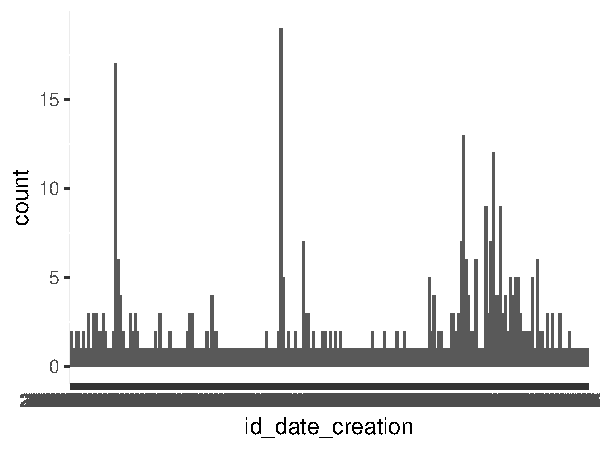
\includegraphics[keepaspectratio]{codebook_data_files/figure-pdf/Var-1-id-date-creation-1.pdf}}

\emini

\begin{itemize}
\tightlist
\item
  Observed factor levels: ``2017-04-01'', ``2017-04-07'',
  ``2017-04-10'', ``2017-04-11'', ``2017-04-12'', ``2017-04-13'',
  ``2017-04-19'', ``2017-04-20'', ``2017-04-22'', ``2017-04-25'',
  ``2017-04-26'', ``2017-04-27'', ``2017-04-28'', ``2017-05-03'',
  ``2017-05-04'', ``2017-05-06'', ``2017-05-07'', ``2017-05-08'',
  ``2017-05-09'', ``2017-05-10'', ``2017-05-11'', ``2017-05-12'',
  ``2017-05-13'', ``2017-05-15'', ``2017-05-16'', ``2017-05-17'',
  ``2017-05-18'', ``2017-05-19'', ``2017-05-20'', ``2017-05-22'',
  ``2017-06-01'', ``2017-06-02'', ``2017-06-05'', ``2017-06-13'',
  ``2017-06-15'', ``2017-06-19'', ``2017-06-20'', ``2017-06-21'',
  ``2017-06-22'', ``2017-06-23'', ``2017-06-24'', ``2017-06-27'',
  ``2017-06-28'', ``2017-06-29'', ``2017-06-30'', ``2017-07-01'',
  ``2017-07-02'', ``2017-07-04'', ``2017-07-05'', ``2017-07-06'',
  ``2017-07-07'', ``2017-07-11'', ``2017-07-12'', ``2017-07-18'',
  ``2017-07-20'', ``2017-07-22'', ``2017-07-23'', ``2017-07-24'',
  ``2017-07-25'', ``2017-07-27'', ``2017-08-01'', ``2017-08-03'',
  ``2017-08-08'', ``2017-08-10'', ``2017-08-17'', ``2017-08-20'',
  ``2017-08-30'', ``2017-08-31'', ``2017-09-02'', ``2017-09-06'',
  ``2017-09-07'', ``2017-09-11'', ``2017-09-20'', ``2017-09-21'',
  ``2017-09-25'', ``2017-09-27'', ``2017-10-05'', ``2017-10-26'',
  ``2017-10-29'', ``2017-11-02'', ``2017-11-09'', ``2017-11-13'',
  ``2017-11-18'', ``2017-11-20'', ``2017-11-21'', ``2017-11-23'',
  ``2017-11-24'', ``2017-11-25'', ``2017-11-26'', ``2017-11-27'',
  ``2017-11-28'', ``2017-11-30'', ``2017-12-04'', ``2017-12-07'',
  ``2017-12-11'', ``2017-12-12'', ``2017-12-13'', ``2017-12-15'',
  ``2017-12-19'', ``2017-12-21'', ``2017-12-22'', ``2017-12-27'',
  ``2017-12-28'', ``2018-01-02'', ``2018-01-04'', ``2018-01-14'',
  ``2018-01-19'', ``2018-01-23'', ``2018-01-27'', ``2018-01-30'',
  ``2018-01-31'', ``2018-02-01'', ``2018-02-03'', ``2018-02-05'',
  ``2018-02-08'', ``2018-02-11'', ``2018-02-12'', ``2018-02-13'',
  ``2018-02-14'', ``2018-02-16'', ``2018-02-20'', ``2018-02-25'',
  ``2018-02-26'', ``2018-03-02'', ``2018-03-03'', ``2018-03-09'',
  ``2018-03-11'', ``2018-03-12'', ``2018-03-28'', ``2018-04-03'',
  ``2018-04-16'', ``2018-04-29'', ``2018-05-03'', ``2018-05-04'',
  ``2018-05-13'', ``2018-05-16'', ``2018-05-31'', ``2018-06-26'',
  ``2018-07-26'', ``2018-07-30'', ``2018-08-09'', ``2018-09-04'',
  ``2018-09-06'', ``2018-09-11'', ``2018-10-23'', ``2018-11-22'',
  ``2018-11-23'', ``2018-11-24'', ``2018-11-26'', ``2018-11-27'',
  ``2018-11-28'', ``2018-11-30'', ``2018-12-01'', ``2018-12-02'',
  ``2018-12-03'', ``2018-12-04'', ``2018-12-05'', ``2018-12-06'',
  ``2018-12-10'', ``2018-12-11'', ``2018-12-12'', ``2018-12-13'',
  ``2018-12-15'', ``2018-12-16'', ``2018-12-17'', ``2018-12-20'',
  ``2018-12-21'', ``2018-12-23'', ``2018-12-24'', ``2018-12-25'',
  ``2018-12-26'', ``2018-12-27'', ``2018-12-28'', ``2018-12-29'',
  ``2018-12-30'', ``2018-12-31'', ``2019-01-01'', ``2019-01-02'',
  ``2019-01-03'', ``2019-01-04'', ``2019-01-05'', ``2019-01-06'',
  ``2019-01-07'', ``2019-01-08'', ``2019-01-09'', ``2019-01-10'',
  ``2019-01-13'', ``2019-01-14'', ``2019-01-15'', ``2019-01-17'',
  ``2019-01-18'', ``2019-01-19'', ``2019-01-21'', ``2019-01-23'',
  ``2019-01-25'', ``2019-01-27'', ``2019-01-29'', ``2019-01-30'',
  ``2019-02-01'', ``2019-02-03'', ``2019-02-14'', ``2019-02-15'',
  ``2019-02-17'', ``2019-02-18'', ``2019-02-26'', ``2019-02-27'',
  ``2019-03-03'', ``2019-03-11'', ``2019-03-19'', ``2019-04-29''.
\end{itemize}

\fullline

\subsection{id\_anonymat}\label{id_anonymat}

\begin{itemize}
\tightlist
\item
  The variable is a key (distinct values for each observation).
\end{itemize}

\fullline

\subsection{id\_centre1}\label{id_centre1}

\bminione

\begin{longtable}[]{@{}lr@{}}
\toprule\noalign{}
Feature & Result \\
\midrule\noalign{}
\endhead
\bottomrule\noalign{}
\endlastfoot
Variable type & integer \\
Number of missing obs. & 37 (8.15 \%) \\
Number of unique values & 46 \\
Median & 221 \\
1st and 3rd quartiles & 202; 251 \\
Min. and max. & 176; 299 \\
\end{longtable}

\emini
\bminitwo

\pandocbounded{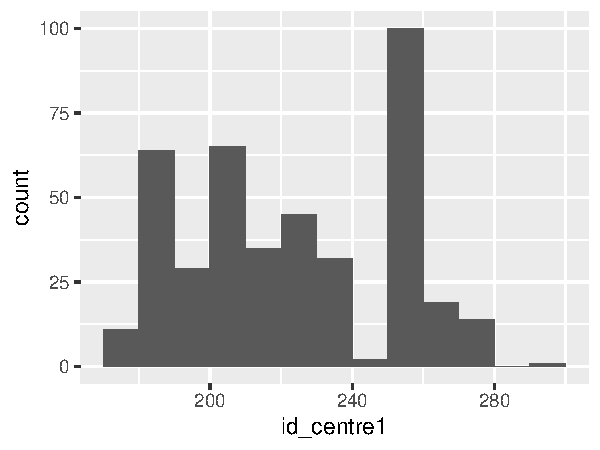
\includegraphics[keepaspectratio]{codebook_data_files/figure-pdf/Var-3-id-centre1-1.pdf}}

\emini

\fullline

\subsection{id\_centre2}\label{id_centre2}

\bminione

\begin{longtable}[]{@{}lr@{}}
\toprule\noalign{}
Feature & Result \\
\midrule\noalign{}
\endhead
\bottomrule\noalign{}
\endlastfoot
Variable type & integer \\
Number of missing obs. & 372 (81.94 \%) \\
Number of unique values & 31 \\
Median & 216 \\
1st and 3rd quartiles & 202; 253 \\
Min. and max. & 178; 299 \\
\end{longtable}

\emini
\bminitwo

\pandocbounded{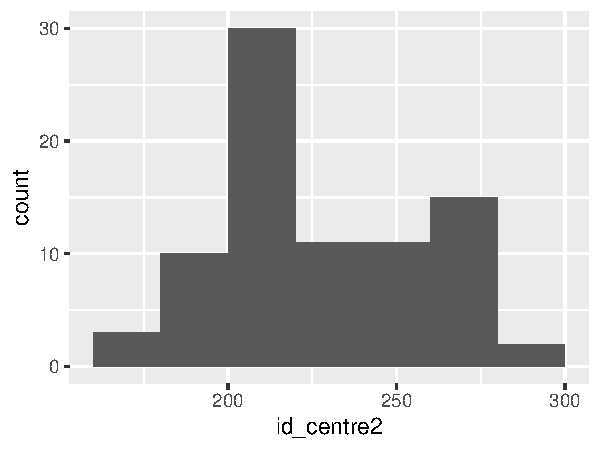
\includegraphics[keepaspectratio]{codebook_data_files/figure-pdf/Var-4-id-centre2-1.pdf}}

\emini

\fullline

\subsection{id\_centre3}\label{id_centre3}

\bminione

\begin{longtable}[]{@{}lr@{}}
\toprule\noalign{}
Feature & Result \\
\midrule\noalign{}
\endhead
\bottomrule\noalign{}
\endlastfoot
Variable type & integer \\
Number of missing obs. & 446 (98.24 \%) \\
Number of unique values & 8 \\
Median & 220 \\
1st and 3rd quartiles & 205.75; 243.25 \\
Min. and max. & 189; 305 \\
\end{longtable}

\emini
\bminitwo

\pandocbounded{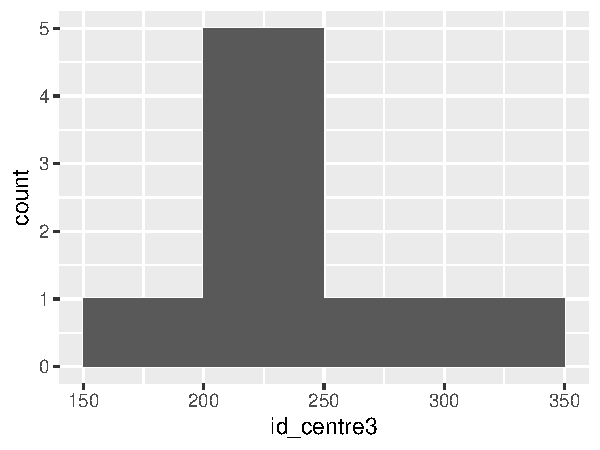
\includegraphics[keepaspectratio]{codebook_data_files/figure-pdf/Var-5-id-centre3-1.pdf}}

\emini

\fullline

\subsection{id\_date\_nais}\label{id_date_nais}

\bminione

\begin{longtable}[]{@{}lr@{}}
\toprule\noalign{}
Feature & Result \\
\midrule\noalign{}
\endhead
\bottomrule\noalign{}
\endlastfoot
Variable type & character \\
Number of missing obs. & 0 (0 \%) \\
Number of unique values & 446 \\
Mode & ``1976-10-15'' \\
\end{longtable}

\emini
\bminitwo

\pandocbounded{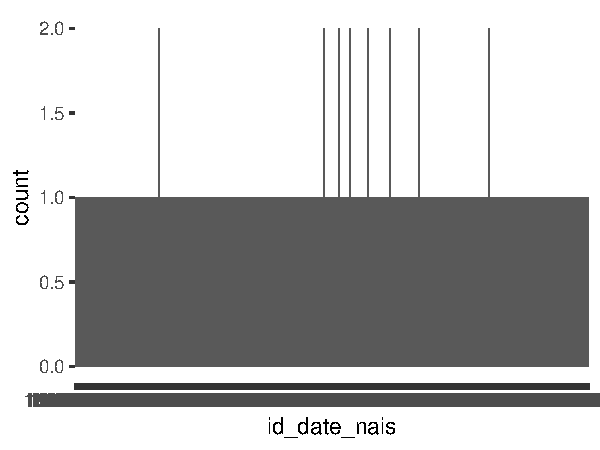
\includegraphics[keepaspectratio]{codebook_data_files/figure-pdf/Var-6-id-date-nais-1.pdf}}

\emini

\begin{itemize}
\tightlist
\item
  Observed factor levels: ``1944-01-12'', ``1944-04-10'',
  ``1950-08-03'', ``1953-05-07'', ``1955-01-07'', ``1958-09-14'',
  ``1959-04-16'', ``1959-06-23'', ``1960-04-30'', ``1960-06-24'',
  ``1961-07-28'', ``1963-04-18'', ``1963-05-09'', ``1963-10-26'',
  ``1964-06-21'', ``1965-04-03'', ``1965-07-26'', ``1966-02-02'',
  ``1966-08-03'', ``1966-08-28'', ``1967-09-04'', ``1967-12-10'',
  ``1968-01-27'', ``1968-05-20'', ``1968-10-11'', ``1968-10-17'',
  ``1968-10-21'', ``1968-12-07'', ``1969-03-19'', ``1969-07-21'',
  ``1969-10-08'', ``1969-11-10'', ``1969-11-13'', ``1970-03-25'',
  ``1970-07-07'', ``1970-08-20'', ``1970-09-04'', ``1971-03-06'',
  ``1971-09-13'', ``1971-12-14'', ``1972-03-21'', ``1972-05-05'',
  ``1972-06-24'', ``1972-08-21'', ``1973-04-27'', ``1973-05-02'',
  ``1973-06-01'', ``1973-07-15'', ``1973-11-20'', ``1974-02-02'',
  ``1974-04-04'', ``1974-06-24'', ``1974-07-16'', ``1974-07-21'',
  ``1974-11-21'', ``1974-11-24'', ``1974-12-13'', ``1975-04-02'',
  ``1975-07-18'', ``1975-07-19'', ``1975-07-31'', ``1975-09-24'',
  ``1975-11-19'', ``1975-12-07'', ``1975-12-23'', ``1976-03-12'',
  ``1976-04-28'', ``1976-06-28'', ``1976-06-30'', ``1976-07-27'',
  ``1976-09-13'', ``1976-09-30'', ``1976-10-15'', ``1976-12-28'',
  ``1977-03-24'', ``1977-04-08'', ``1977-04-09'', ``1977-04-23'',
  ``1977-05-01'', ``1977-05-21'', ``1977-05-31'', ``1977-06-09'',
  ``1977-07-25'', ``1977-08-26'', ``1977-09-17'', ``1977-10-01'',
  ``1977-10-07'', ``1977-10-29'', ``1977-12-20'', ``1978-02-25'',
  ``1978-04-06'', ``1978-04-15'', ``1978-05-20'', ``1978-05-21'',
  ``1978-10-04'', ``1978-12-19'', ``1979-03-01'', ``1979-04-30'',
  ``1979-05-05'', ``1979-06-08'', ``1979-06-10'', ``1979-07-07'',
  ``1979-07-10'', ``1979-07-14'', ``1979-07-22'', ``1979-08-07'',
  ``1979-08-17'', ``1979-08-29'', ``1979-09-12'', ``1979-09-25'',
  ``1979-11-01'', ``1980-01-27'', ``1980-04-13'', ``1980-05-16'',
  ``1980-05-24'', ``1980-07-09'', ``1980-09-18'', ``1980-12-06'',
  ``1980-12-18'', ``1981-01-04'', ``1981-01-23'', ``1981-01-28'',
  ``1981-03-23'', ``1981-04-25'', ``1981-05-08'', ``1981-05-15'',
  ``1981-07-07'', ``1981-07-11'', ``1981-08-03'', ``1981-08-07'',
  ``1981-08-08'', ``1981-08-11'', ``1981-08-24'', ``1981-10-06'',
  ``1981-11-13'', ``1981-11-17'', ``1981-11-20'', ``1981-11-25'',
  ``1981-12-11'', ``1982-02-24'', ``1982-03-30'', ``1982-05-05'',
  ``1982-05-07'', ``1982-05-26'', ``1982-06-14'', ``1982-10-27'',
  ``1982-11-01'', ``1982-11-06'', ``1982-11-17'', ``1982-11-24'',
  ``1982-12-01'', ``1983-01-22'', ``1983-01-30'', ``1983-02-11'',
  ``1983-03-03'', ``1983-03-14'', ``1983-03-21'', ``1983-03-28'',
  ``1983-05-04'', ``1983-05-05'', ``1983-05-26'', ``1983-06-05'',
  ``1983-08-10'', ``1983-08-15'', ``1983-09-21'', ``1983-10-11'',
  ``1983-11-28'', ``1984-01-10'', ``1984-03-05'', ``1984-04-01'',
  ``1984-04-22'', ``1984-05-01'', ``1984-05-23'', ``1984-05-25'',
  ``1984-06-14'', ``1984-06-22'', ``1984-07-18'', ``1984-09-04'',
  ``1984-09-18'', ``1984-09-21'', ``1984-12-28'', ``1985-03-29'',
  ``1985-05-15'', ``1985-05-22'', ``1985-06-13'', ``1985-06-20'',
  ``1985-06-21'', ``1985-07-09'', ``1985-07-20'', ``1985-08-03'',
  ``1985-08-05'', ``1985-08-11'', ``1985-08-12'', ``1985-08-23'',
  ``1985-10-28'', ``1985-11-05'', ``1985-12-04'', ``1986-02-17'',
  ``1986-02-24'', ``1986-04-16'', ``1986-05-11'', ``1986-05-13'',
  ``1986-06-17'', ``1986-06-19'', ``1986-06-21'', ``1986-07-09'',
  ``1986-07-18'', ``1986-10-03'', ``1986-10-24'', ``1986-11-07'',
  ``1986-11-28'', ``1986-12-30'', ``1987-02-09'', ``1987-02-27'',
  ``1987-03-03'', ``1987-03-06'', ``1987-03-10'', ``1987-04-12'',
  ``1987-05-15'', ``1987-05-16'', ``1987-05-27'', ``1987-06-01'',
  ``1987-07-06'', ``1987-07-11'', ``1987-08-20'', ``1987-08-21'',
  ``1987-10-05'', ``1987-11-03'', ``1987-11-13'', ``1987-11-19'',
  ``1988-01-15'', ``1988-01-19'', ``1988-01-22'', ``1988-02-14'',
  ``1988-03-12'', ``1988-03-27'', ``1988-04-29'', ``1988-05-12'',
  ``1988-05-18'', ``1988-05-28'', ``1988-06-12'', ``1988-06-27'',
  ``1988-07-22'', ``1988-07-26'', ``1988-08-11'', ``1988-08-14'',
  ``1988-08-24'', ``1988-08-30'', ``1988-09-06'', ``1988-09-10'',
  ``1988-10-20'', ``1988-11-15'', ``1988-12-21'', ``1989-01-14'',
  ``1989-01-21'', ``1989-03-20'', ``1989-03-23'', ``1989-04-03'',
  ``1989-05-07'', ``1989-06-15'', ``1989-07-01'', ``1989-07-07'',
  ``1989-07-26'', ``1989-08-03'', ``1989-08-09'', ``1989-08-23'',
  ``1989-09-09'', ``1989-09-19'', ``1989-09-20'', ``1989-11-02'',
  ``1989-11-16'', ``1989-12-27'', ``1989-12-29'', ``1990-01-15'',
  ``1990-01-30'', ``1990-02-08'', ``1990-02-26'', ``1990-04-06'',
  ``1990-04-07'', ``1990-04-09'', ``1990-05-07'', ``1990-06-03'',
  ``1990-06-06'', ``1990-06-08'', ``1990-06-12'', ``1990-06-13'',
  ``1990-07-04'', ``1990-08-07'', ``1990-08-16'', ``1990-08-18'',
  ``1990-08-27'', ``1990-11-29'', ``1990-12-28'', ``1991-01-11'',
  ``1991-01-26'', ``1991-01-27'', ``1991-02-10'', ``1991-02-14'',
  ``1991-03-15'', ``1991-03-24'', ``1991-04-20'', ``1991-06-16'',
  ``1991-06-24'', ``1991-07-03'', ``1991-08-24'', ``1991-08-30'',
  ``1991-11-04'', ``1991-12-01'', ``1991-12-02'', ``1991-12-07'',
  ``1991-12-09'', ``1991-12-12'', ``1991-12-17'', ``1992-01-04'',
  ``1992-01-24'', ``1992-03-02'', ``1992-03-27'', ``1992-04-12'',
  ``1992-04-25'', ``1992-06-16'', ``1992-07-02'', ``1992-07-06'',
  ``1992-08-03'', ``1992-10-01'', ``1992-12-08'', ``1993-01-17'',
  ``1993-01-21'', ``1993-03-05'', ``1993-04-07'', ``1993-04-27'',
  ``1993-06-01'', ``1993-07-08'', ``1993-07-17'', ``1993-08-26'',
  ``1993-09-02'', ``1993-09-03'', ``1993-09-30'', ``1993-10-06'',
  ``1993-10-15'', ``1993-10-25'', ``1993-10-28'', ``1993-11-01'',
  ``1993-11-18'', ``1993-12-08'', ``1994-01-15'', ``1994-02-26'',
  ``1994-06-08'', ``1994-06-15'', ``1994-07-02'', ``1994-07-05'',
  ``1994-07-07'', ``1994-07-21'', ``1994-09-23'', ``1994-10-22'',
  ``1994-12-14'', ``1995-01-24'', ``1995-02-01'', ``1995-02-20'',
  ``1995-02-21'', ``1995-03-06'', ``1995-03-08'', ``1995-03-10'',
  ``1995-06-28'', ``1995-07-28'', ``1995-08-21'', ``1995-09-22'',
  ``1995-09-23'', ``1996-02-09'', ``1996-02-15'', ``1996-05-03'',
  ``1996-06-03'', ``1996-06-18'', ``1996-08-08'', ``1996-09-10'',
  ``1996-10-09'', ``1996-10-26'', ``1996-11-05'', ``1996-12-08'',
  ``1997-01-01'', ``1997-01-10'', ``1997-02-25'', ``1997-03-26'',
  ``1997-04-18'', ``1997-04-29'', ``1997-04-30'', ``1997-05-20'',
  ``1997-05-26'', ``1997-07-29'', ``1997-08-18'', ``1997-08-31'',
  ``1997-09-02'', ``1997-09-11'', ``1997-09-27'', ``1997-10-24'',
  ``1997-12-14'', ``1997-12-27'', ``1998-04-01'', ``1998-04-06'',
  ``1998-04-15'', ``1998-04-20'', ``1998-06-03'', ``1998-10-21'',
  ``1998-12-17'', ``1999-01-27'', ``1999-02-26'', ``1999-05-21'',
  ``1999-05-25'', ``1999-05-28'', ``1999-06-25'', ``1999-07-03'',
  ``1999-07-06'', ``1999-07-23'', ``1999-07-31'', ``1999-08-25'',
  ``1999-09-16'', ``1999-10-28'', ``1999-11-18'', ``2000-02-17'',
  ``2000-04-19'', ``2000-04-26'', ``2000-05-03'', ``2000-07-12'',
  ``2000-10-26'', ``2001-05-07'', ``2001-06-25'', ``2001-09-06'',
  ``2001-10-05'', ``2001-10-07'', ``2001-11-04'', ``2001-11-08'',
  ``2001-12-29'', ``2002-01-30'', ``2002-03-07'', ``2002-05-30'',
  ``2002-08-26'', ``2002-09-21'', ``2002-11-05'', ``2002-12-06'',
  ``2003-02-24'', ``2003-06-27'', ``2003-10-20'', ``2004-01-10'',
  ``2004-01-19'', ``2004-03-14'', ``2004-05-25'', ``2004-11-20''.
\end{itemize}

\fullline

\subsection{id\_dep\_nais}\label{id_dep_nais}

\bminione

\begin{longtable}[]{@{}lr@{}}
\toprule\noalign{}
Feature & Result \\
\midrule\noalign{}
\endhead
\bottomrule\noalign{}
\endlastfoot
Variable type & integer \\
Number of missing obs. & 64 (14.1 \%) \\
Number of unique values & 77 \\
Median & 59 \\
1st and 3rd quartiles & 37; 74 \\
Min. and max. & 1; 974 \\
\end{longtable}

\emini
\bminitwo

\pandocbounded{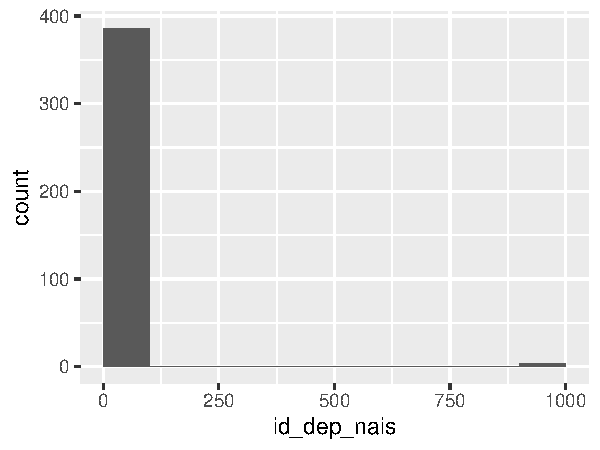
\includegraphics[keepaspectratio]{codebook_data_files/figure-pdf/Var-7-id-dep-nais-1.pdf}}

\emini

\fullline

\subsection{id\_lieu\_nais}\label{id_lieu_nais}

\bminione

\begin{longtable}[]{@{}lr@{}}
\toprule\noalign{}
Feature & Result \\
\midrule\noalign{}
\endhead
\bottomrule\noalign{}
\endlastfoot
Variable type & integer \\
Number of missing obs. & 0 (0 \%) \\
Number of unique values & 2 \\
Median & 1 \\
1st and 3rd quartiles & 1; 1 \\
Min. and max. & 1; 2 \\
\end{longtable}

\emini
\bminitwo

\pandocbounded{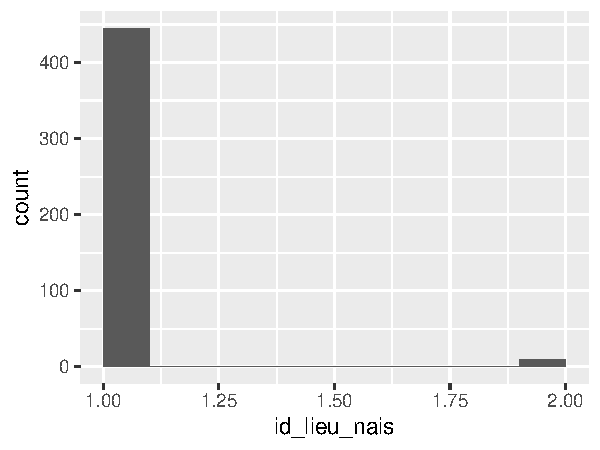
\includegraphics[keepaspectratio]{codebook_data_files/figure-pdf/Var-8-id-lieu-nais-1.pdf}}

\emini

\fullline

\subsection{id\_nom}\label{id_nom}

\bminione

\begin{longtable}[]{@{}lr@{}}
\toprule\noalign{}
Feature & Result \\
\midrule\noalign{}
\endhead
\bottomrule\noalign{}
\endlastfoot
Variable type & character \\
Number of missing obs. & 0 (0 \%) \\
Number of unique values & 297 \\
Mode & ``CHA'' \\
\end{longtable}

\emini
\bminitwo

\pandocbounded{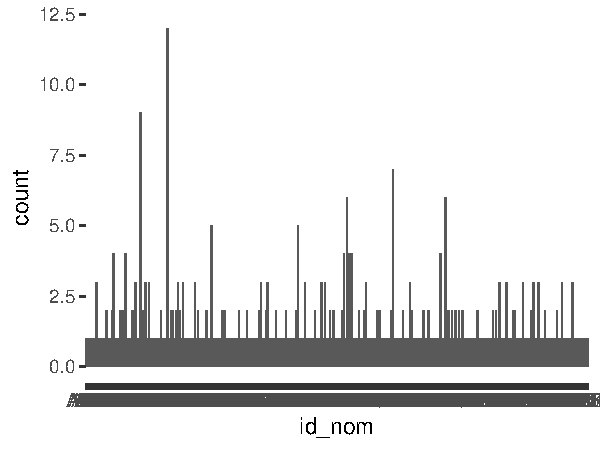
\includegraphics[keepaspectratio]{codebook_data_files/figure-pdf/Var-9-id-nom-1.pdf}}

\emini

\begin{itemize}
\tightlist
\item
  Observed factor levels: ``AGN'', ``AGR'', ``AHA'', ``ALB'', ``ALC'',
  ``ALG'', ``ALL'', ``AMI'', ``AMO'', ``AMZ'', ``AND'', ``ARN'',
  ``ARR'', ``ASA'', ``AUG'', ``BAC'', ``BAR'', ``BAT'', ``BAU'',
  ``BEA'', ``BEC'', ``BEL'', ``BEN'', ``BER'', ``BIG'', ``BIL'',
  ``BIN'', ``BLA'', ``BOI'', ``BON'', ``Bos'', ``BOS'', ``BOU'',
  ``BRA'', ``BRE'', ``BRI'', ``BRO'', ``BRU'', ``BUH'', ``BUO'',
  ``CAD'', ``CAL'', ``CAS'', ``CAT'', ``CAU'', ``CAZ'', ``CEL'',
  ``CER'', ``CHA'', ``CHE'', ``CHO'', ``CLE'', ``COD'', ``COE'',
  ``COL'', ``CON'', ``Cou'', ``COU'', ``CRE'', ``CUP'', ``CUY'',
  ``CZE'', ``CZI'', ``DAA'', ``DAL'', ``DAM'', ``DAR'', ``DAS'',
  ``DAU'', ``DEB'', ``DEC'', ``DEL'', ``DEM'', ``DEO'', ``DES'',
  ``DIE'', ``DIS'', ``DOR'', ``DOU'', ``DRU'', ``DUB'', ``DUC'',
  ``DUF'', ``DUG'', ``DUP'', ``DUR'', ``DUT'', ``DUV'', ``EGO'',
  ``ELI'', ``EME'', ``ENJ'', ``EST'', ``FAL'', ``FAT'', ``FAU'',
  ``FAV'', ``FER'', ``FIA'', ``FLA'', ``FLE'', ``FOL'', ``FON'',
  ``FOR'', ``FOU'', ``FUL'', ``GAI'', ``GAL'', ``GAR'', ``GAV'',
  ``GED'', ``GEL'', ``GEN'', ``GER'', ``GHE'', ``GIB'', ``GIC'',
  ``GIL'', ``GIR'', ``GLO'', ``GOI'', ``GOU'', ``GRA'', ``GRO'',
  ``GUE'', ``GUI'', ``GUR'', ``HAY'', ``HEM'', ``HER'', ``HID'',
  ``HOU'', ``HUY'', ``JAC'', ``JAN'', ``JEA'', ``JEN'', ``JOC'',
  ``JOS'', ``JOU'', ``JUH'', ``KER'', ``KOP'', ``KUP'', ``LAB'',
  ``LAC'', ``LAD'', ``LAF'', ``LAL'', ``LAM'', ``LAN'', ``LAP'',
  ``LAU'', ``LAV'', ``LEB'', ``LEC'', ``LEF'', ``LEG'', ``LEH'',
  ``LEM'', ``LEN'', ``LEO'', ``LEP'', ``LEQ'', ``LER'', ``LET'',
  ``LEV'', ``LIO'', ``LOE'', ``LOR'', ``LOT'', ``LOU'', ``LOY'',
  ``LUC'', ``LUM'', ``MAA'', ``MAE'', ``MAG'', ``MAI'', ``MAL'',
  ``MAN'', ``MAR'', ``MAS'', ``MAU'', ``MET'', ``MIC'', ``MIK'',
  ``MIL'', ``MIR'', ``MLY'', ``MOL'', ``MON'', ``MOR'', ``MOS'',
  ``MUC'', ``MUH'', ``NAM'', ``NEH'', ``NER'', ``NGU'', ``NIC'',
  ``NIO'', ``NOE'', ``NOI'', ``ORY'', ``OST'', ``OUL'', ``PAL'',
  ``PAP'', ``PAR'', ``PAT'', ``PAY'', ``PER'', ``PET'', ``PIE'',
  ``PIG'', ``PIL'', ``PIT'', ``POI'', ``POL'', ``PON'', ``POR'',
  ``POU'', ``POY'', ``PRE'', ``PRI'', ``QUE'', ``RAD'', ``RAF'',
  ``RAM'', ``RAV'', ``RAY'', ``REB'', ``RED'', ``REG'', ``REM'',
  ``REN'', ``RER'', ``REZ'', ``RIB'', ``RIC'', ``RIE'', ``RIP'',
  ``RIT'', ``ROB'', ``ROC'', ``ROL'', ``ROS'', ``ROU'', ``RUB'',
  ``RUF'', ``RUY'', ``SAL'', ``SAN'', ``SAV'', ``SAY'', ``SCH'',
  ``SEB'', ``SEI'', ``SEK'', ``SEN'', ``SEV'', ``SIB'', ``SIL'',
  ``SIM'', ``SIS'', ``SOL'', ``SOU'', ``SOY'', ``STR'', ``TAI'',
  ``TAL'', ``TAM'', ``TES'', ``THE'', ``THI'', ``THO'', ``TIS'',
  ``TRI'', ``TRU'', ``USH'', ``VAL'', ``VAN'', ``VER'', ``VIA'',
  ``VIG'', ``VIO'', ``VIT'', ``VUL'', ``VUY'', ``WAL'', ``WEI'',
  ``WER'', ``WYO'', ``XAV'', ``YAK'', ``ZAH''.
\end{itemize}

\fullline

\subsection{id\_nom\_jeune}\label{id_nom_jeune}

\bminione

\begin{longtable}[]{@{}lr@{}}
\toprule\noalign{}
Feature & Result \\
\midrule\noalign{}
\endhead
\bottomrule\noalign{}
\endlastfoot
Variable type & character \\
Number of missing obs. & 322 (70.93 \%) \\
Number of unique values & 106 \\
Mode & ``LEF'' \\
\end{longtable}

\emini
\bminitwo

\pandocbounded{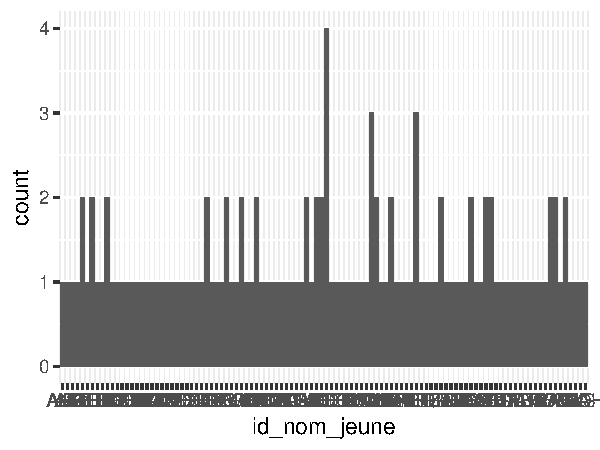
\includegraphics[keepaspectratio]{codebook_data_files/figure-pdf/Var-10-id-nom-jeune-1.pdf}}

\emini

\begin{itemize}
\tightlist
\item
  Observed factor levels: ``ALL'', ``ANG'', ``ASS'', ``AV'', ``BAR'',
  ``BEL'', ``BER'', ``BEU'', ``BIL'', ``BRE'', ``BRI'', ``BRU'',
  ``CAL'', ``CHA'', ``CHE'', ``CIG'', ``CLA'', ``COI'', ``COL'',
  ``Cou'', ``CUY'', ``CZE'', ``DAL'', ``DAS'', ``DEB'', ``DEC'',
  ``DEL'', ``DES'', ``DEV'', ``DUB'', ``DUF'', ``DUM'', ``FAL'',
  ``FOR'', ``FOU'', ``FUL'', ``GAU'', ``GOI'', ``GUG'', ``GUI'',
  ``HAN'', ``HEM'', ``HOY'', ``IVA'', ``JEA'', ``JEF'', ``JOL'',
  ``JOU'', ``KER'', ``LAG'', ``LAU'', ``LEC'', ``LED'', ``LEF'',
  ``LEG'', ``LEO'', ``LEP'', ``LIC'', ``LOC'', ``LOI'', ``LOU'',
  ``MAH'', ``MAR'', ``MIL'', ``MOK'', ``MON'', ``MOR'', ``NEH'',
  ``ORL'', ``PAR'', ``PAU'', ``PER'', ``PIT'', ``PIZ'', ``PRI'',
  ``PRO'', ``QUE'', ``RAY'', ``RED'', ``REG'', ``RIE'', ``ROS'',
  ``ROU'', ``RUY'', ``SAG'', ``SAL'', ``SEI'', ``SIS'', ``SIT'',
  ``SOL'', ``STA'', ``TAU'', ``TAV'', ``TEJ'', ``THI'', ``THO'',
  ``TIS'', ``TOI'', ``TOU'', ``VAN'', ``VEN'', ``VIA'', ``VIL'',
  ``VIO'', ``VIS'', ``ZAH''.
\end{itemize}

\fullline

\subsection{id\_prenom}\label{id_prenom}

\bminione

\begin{longtable}[]{@{}lr@{}}
\toprule\noalign{}
Feature & Result \\
\midrule\noalign{}
\endhead
\bottomrule\noalign{}
\endlastfoot
Variable type & character \\
Number of missing obs. & 6 (1.32 \%) \\
Number of unique values & 98 \\
Mode & ``MA'' \\
\end{longtable}

\emini
\bminitwo

\pandocbounded{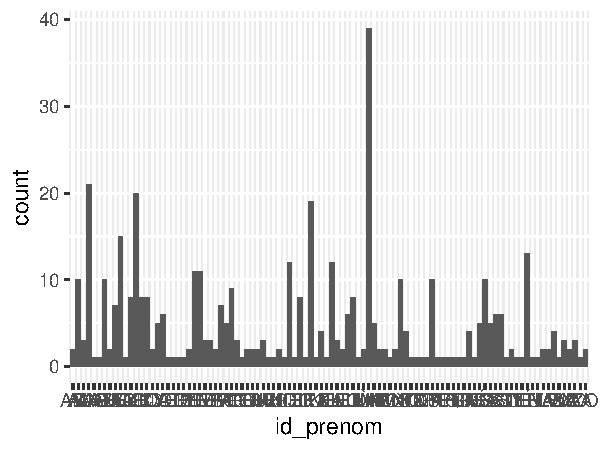
\includegraphics[keepaspectratio]{codebook_data_files/figure-pdf/Var-11-id-prenom-1.pdf}}

\emini

\begin{itemize}
\tightlist
\item
  Observed factor levels: ``AD'', ``AL'', ``AM'', ``AN'', ``AS'',
  ``AT'', ``AU'', ``BA'', ``BE'', ``CA'', ``Ce'', ``CE'', ``CH'',
  ``CL'', ``CO'', ``CY'', ``DA'', ``DE'', ``DI'', ``DO'', ``DR'',
  ``DY'', ``ED'', ``EL'', ``EM'', ``ER'', ``ES'', ``EV'', ``FA'',
  ``FL'', ``FR'', ``GE'', ``GH'', ``GR'', ``GU'', ``GW'', ``HE'',
  ``HU'', ``IN'', ``IS'', ``JC'', ``JE'', ``JI'', ``JO'', ``JP'',
  ``JU'', ``KA'', ``KE'', ``KI'', ``LA'', ``LE'', ``LI'', ``LO'',
  ``LU'', ``LÙ'', ``LY'', ``MA'', ``ME'', ``MI'', ``MO'', ``MU'',
  ``MY'', ``NI'', ``NO'', ``OD'', ``OL'', ``OP'', ``OU'', ``PA'',
  ``PE'', ``PH'', ``PI'', ``PL'', ``QU'', ``RA'', ``RE'', ``RÉ'',
  ``RO'', ``SA'', ``SE'', ``SO'', ``ST'', ``SU'', ``SY'', ``TE'',
  ``TÉ'', ``TH'', ``TI'', ``UL'', ``VA'', ``VE'', ``VI'', ``WI'',
  ``XA'', ``YA'', ``YO'', ``ZA'', ``ZO''.
\end{itemize}

\fullline

\subsection{id\_sexe}\label{id_sexe}

\bminione

\begin{longtable}[]{@{}lr@{}}
\toprule\noalign{}
Feature & Result \\
\midrule\noalign{}
\endhead
\bottomrule\noalign{}
\endlastfoot
Variable type & integer \\
Number of missing obs. & 0 (0 \%) \\
Number of unique values & 2 \\
Median & 2 \\
1st and 3rd quartiles & 1; 2 \\
Min. and max. & 1; 2 \\
\end{longtable}

\emini
\bminitwo

\pandocbounded{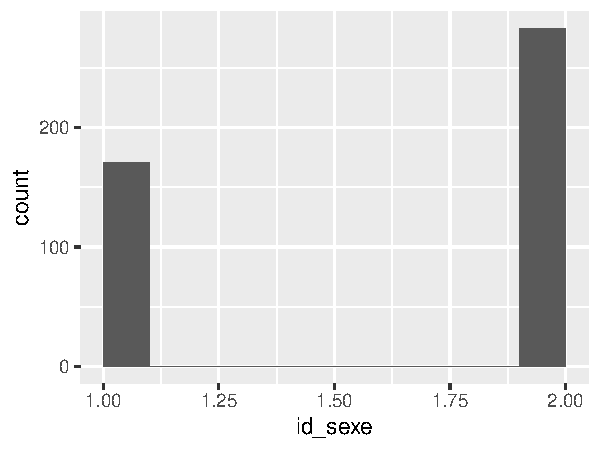
\includegraphics[keepaspectratio]{codebook_data_files/figure-pdf/Var-12-id-sexe-1.pdf}}

\emini

\fullline

\subsection{id\_type}\label{id_type}

\begin{itemize}
\tightlist
\item
  The variable only takes one (non-missing) value: ``P''. The variable
  contains 0 \% missing observations.
\end{itemize}

\fullline

\subsection{id\_age}\label{id_age}

\bminione

\begin{longtable}[]{@{}lr@{}}
\toprule\noalign{}
Feature & Result \\
\midrule\noalign{}
\endhead
\bottomrule\noalign{}
\endlastfoot
Variable type & integer \\
Number of missing obs. & 0 (0 \%) \\
Number of unique values & 50 \\
Median & 30 \\
1st and 3rd quartiles & 25; 38 \\
Min. and max. & 14; 74 \\
\end{longtable}

\emini
\bminitwo

\pandocbounded{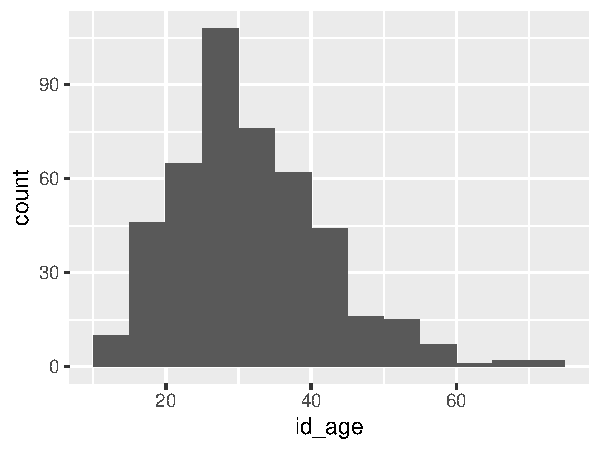
\includegraphics[keepaspectratio]{codebook_data_files/figure-pdf/Var-14-id-age-1.pdf}}

\emini

\fullline

\subsection{id\_tab\_db}\label{id_tab_db}

\bminione

\begin{longtable}[]{@{}lr@{}}
\toprule\noalign{}
Feature & Result \\
\midrule\noalign{}
\endhead
\bottomrule\noalign{}
\endlastfoot
Variable type & integer \\
Number of missing obs. & 0 (0 \%) \\
Number of unique values & 2 \\
Median & 0 \\
1st and 3rd quartiles & 0; 0 \\
Min. and max. & 0; 1 \\
\end{longtable}

\emini
\bminitwo

\pandocbounded{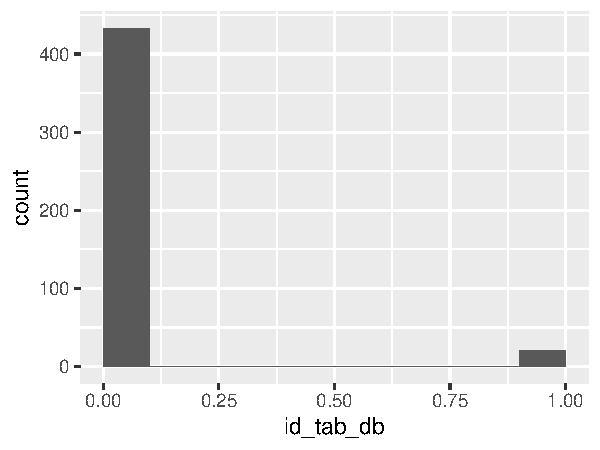
\includegraphics[keepaspectratio]{codebook_data_files/figure-pdf/Var-15-id-tab-db-1.pdf}}

\emini

\fullline

\subsection{id\_sep}\label{id_sep}

\bminione

\begin{longtable}[]{@{}lr@{}}
\toprule\noalign{}
Feature & Result \\
\midrule\noalign{}
\endhead
\bottomrule\noalign{}
\endlastfoot
Variable type & character \\
Number of missing obs. & 433 (95.37 \%) \\
Number of unique values & 21 \\
Mode & ``BTWKW\_WELSE'' \\
\end{longtable}

\emini
\bminitwo

\pandocbounded{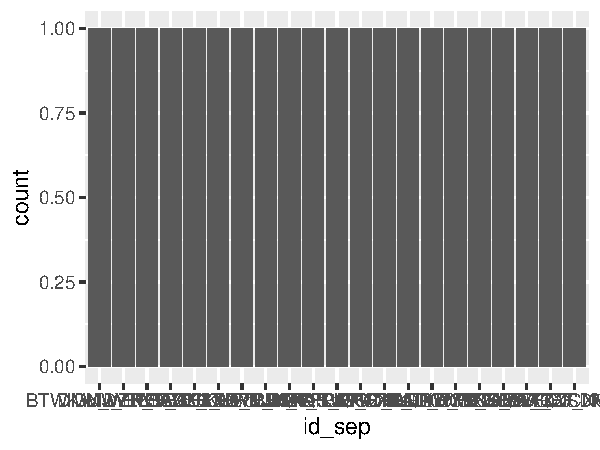
\includegraphics[keepaspectratio]{codebook_data_files/figure-pdf/Var-16-id-sep-1.pdf}}

\emini

\begin{itemize}
\tightlist
\item
  Observed factor levels: ``BTWKW\_WELSE'', ``DMLIJ\_HWVVT'',
  ``DNWZK\_TEOOO'', ``DYTKD\_ZHARX'', ``FEKTM\_KLIFT'',
  ``GAYSH\_XWGEQ'', ``GCXSD\_VJHNY'', ``GXHPT\_KRYPP'',
  ``HSOMH\_GFPQP'', ``IBWZT\_SJERR'', ``JNYQS\_WYONK'',
  ``KAHVO\_FRBQR'', ``LJHGZ\_IMTKF'', ``MGDIU\_DYHCM'',
  ``OXKAC\_OFXOJ'', ``RJLOD\_GRXQD'', ``RKWYE\_DBRRR'',
  ``VMPCE\_YDQEF'', ``WNGMA\_QZSDI'', ``YASAA\_WCNVO'',
  ``ZWFGU\_XCTKR''.
\end{itemize}

\fullline

\subsection{id\_link}\label{id_link}

\begin{itemize}
\tightlist
\item
  The variable is a key (distinct values for each observation).
\end{itemize}

\fullline

\subsection{sc\_commentaires}\label{sc_commentaires}

\bminione

\begin{longtable}[]{@{}lr@{}}
\toprule\noalign{}
Feature & Result \\
\midrule\noalign{}
\endhead
\bottomrule\noalign{}
\endlastfoot
Variable type & character \\
Number of missing obs. & 379 (83.48 \%) \\
Number of unique values & 73 \\
Mode & ``RAS'' \\
\end{longtable}

\emini
\bminitwo

\pandocbounded{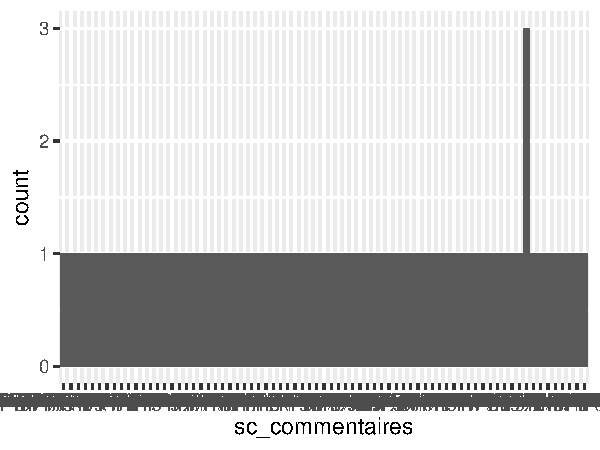
\includegraphics[keepaspectratio]{codebook_data_files/figure-pdf/Var-18-sc-commentaires-1.pdf}}

\emini

\begin{itemize}
\tightlist
\item
  Observed factor levels: ``-'', ``2002 BTS compta 2006 BTS Management
  des unités commerciales ne trouvant pas de travail après mon bts
  compta, j'ai décidé de reprendre mes études en 2004, en alternance,
  pour avoir la garantie d'avoir une expérience professionnelle'', ``A
  cette époque je savais pas que j'avais la mucoviscidose'', ``A mon
  époque on parlait de PAI, j'imagine que c'est l'équivalent du PPS ?
  J'ai fait une demande de tiers temps lors des concours aux grandes
  écoles, je pense que le questionnaire Scolarité peut aborder ce sujet
  de faire une année de scolarité en deux ans, ou les tiers temps pour
  les examens'', ``Actuellement en école d?infirmière'', ``après mon
  obtention du bac en 2004, puis mes 2 années de DUT (2004-2006), je
  suis parti en BTS en alternance (2006-2008) enfin j'ai terminé (à ce
  jour) ma scolarité par une licence professionnelle en alternance
  (2008-2009)'', ``Aucun'', ``Baccalaureat Littéraire obtenu en 1997
  lors d ema dernière activité professionnelle en 2014, j'ai souhaité
  reprendre mes études, et ai do c en parallèle de mon travail effectué
  une VAE (validation des acquis de l'expérience) et obtenir mon BTS à
  37 ans.'', ``bien'', ``Ce questionnaire ne prend pas en compte le fait
  d'un diagnostic tarif de la muco par le corps médical. J'ai été
  diagnostiqué qu'en 2009. Ma scolarité a donc été beaucoup impacté par
  l'ensemble de symptômes liés à la muco mais que les médecins indiqués
  être liés à mon inconscient (toux, mucus, fatigue, maigreur, stress,
  associable, sinusites, allergies\ldots). Petit, les médecins m'ont dit
  que je me créée l'ensemble des symptomes et m'ont envoyé voir des
  psys. Ma scolarité a donc été éprouvante puisque j'étais persuadé que
  tout était ma faute, que j'étais plus faible que les autres. J'ai donc
  tout fait pour avoir l'ensemble de mes diplomes mais ai du mettre de
  côté ma vie sociale (impossible de suivre les cours à l'université et
  de sortir le soir).'', ``Diagnostique tardif de mucoviscidose, non
  détecté pendant la scolarité'', ``Difficile de me rapeller de ma
  scolarité en primaire et du nombre de périodes d'interruptions. Mes
  parents, surtout ma mère, ont rencontré tous mes enseignants et leurs
  directeur à l'époque. Le projet personnalisé de scolarisation (PPS)
  n'existait pas à mon époque. Le questionnaire pourrait également
  demandé si un Projet d'Accueil Individualisé (PAI) a été mis en
  place.'', ``Diplôme d'architecte + Maîtrise d'oeuvre'', ``En dehors de
  la maternelle, j'ai débuté ma scolarité en CE1 car j'ai sauté la
  classe de CP. Concernant l'interruption de scolarité enregistrée, je
  n'ai pas réussi à indiquer la classe interrompue (1ère) mais seulement
  la classe reprise (1ère).'', ``En primaire, au collège (2 fois), et
  une fois au lycée, j'ai interrompu ma scolarité pour réaliser des
  cures d'antibiotiques par intraveineuse que j'ai pu effectuer à
  domicile. Il s'agissait de périodes n'excédant pas 15 jours. Au début,
  j'ai essayé d'aller en classe avec mon cathéter dans le bras, mais
  c'était assez embarrassant pour moi (regard des autres, il fallait que
  je fasse attention à ne pas me cogner le bras\ldots). Puis, les veines
  de mon bras gauche se sont mises à toutes claquer, il était devenu
  inutilisable. Avec le cathéter au bras droit, il ne servait à rien
  d'aller en classe pendant les cures puisque je ne pouvais pas écrire.
  Mais cela m'a évité l'embarras de devoir affronter mes camarades de
  classe, je ne voulais surtout pas que l'on se rende compte de quoi que
  ce soit (je cache ma maladie depuis toujours, le plus possible). De
  plus, les cures débutant très tôt le matin, se terminant très tard le
  soir, j'étais fatiguée, donc c'était mieux pour moi de rester à la
  maison. J'avais deux amies, auxquelles j'avais confié ma situation et
  qui me passaient leurs cours et les devoirs à faire, afin que je ne
  prenne pas de retard, et ma mère m'a aidée à les recopier. J'ai eu la
  chance d'avoir ma mère à la maison, elle m'a beaucoup aidée, soutenue,
  elle a fait en sorte que je puisse faire mes cures à la maison dès la
  première. Au collège j'ai également dû être hospitalisée une semaine à
  cause d'une subocclusion intestinale, mais c'est la seule
  hospitalisation que j'ai subie.'', ``Il est très complet et bien
  construit. Il est difficile de remémorer les arrêt d'école de plus de
  1 mois tant ils sont nombreux pour des cures I.V. suite à des virus
  comme la grippe ou une simple angine.'', ``il m est arrive d avoir ete
  absente durant 3 semaines'', ``Il manque une partie concernant une
  aide durant les années Post Bac.'', ``Il y a des périodes de l'année
  ou aller à l'école est difficile à cause de la fatigue ou de
  l'encombrement'', ``Interruption de mon année de seconde générale puis
  reprise en septembre de l'année d'après un CAP esthétique en 2 ans que
  j'ai obtenu, puis un bac pro Esthétique en alternance en 2 ans ou j'ai
  du m'arrêter au bout d'une année car trop éprouvant physiquement, puis
  j'ai travaillé en parfumerie 1 an ensuite j'ai eu un enfant et me suis
  arrêtée 3 ans, j'ai aussi repris un bac immobilier en 1 an, obtenu et
  je travaille depuis 1 an comme négociatrice immobilier.'', ``J'ai
  appris que j'avais la mucoviscidose quand j'étais en seconde, avant
  personne ne l'avait dépisté et certains médecins pensaient que c'était
  psychosommatique.'', ``J'ai arrêté mes études car mon état s'est
  dégradé et depuis j'ai été greffée. Je ne pense pas reprendre mes
  études mais je vais certainement devoir reprendre une formation plus
  ou moins longue mais je ne sais absolument pas dans quel domaine.'',
  ``j'ai arrêté une première fois mes étude en 1996 avec un DUT en poche
  avant de les reprendre en tant que salarié entre 2002 et 2004 par
  correspondance et entre 2002 et 2004 dans le cadre d'un congé
  individuel de formation pour obtenir un diplôme d'ingénieur.'', ``J'ai
  bénéficié d'un tiers temps supplémentaire pour passer mes examens à
  partir du baccalauréat et pour mes études supérieures (DEUG et
  LICENCE)'', ``j'ai également le niveau licence psychologie'', ``J'ai
  été dépistée à l'age de 15 ans. mon état n'était pas grave, j'ai voulu
  terminer ma scolarité avant de commencer à me soigner.'', ``J'ai été
  diagnostiqué à 16 ans donc en primaire et au collège je ne savais pas
  que j'avais la muco'', ``j'ai été souvent malade durant ma scolarité
  mais on ne m'a diagnostiqué la mucoviscidose quand 2014, donc mes
  parents et moi même ne savions pas qu'il sa'gissait de cette
  maladie.'', ``j'ai eu un tiers temps pour mon examen du BTS'', ``J'ai
  fais 2 ans de Brevet enseignement commercial après le BEPC mais je
  n'ai pas obtenu le diplôme en 1968.'', ``J'ai fais un BEPA services
  aux personnes de 2010 à 2012. Puis n'ayant pu aller en établissement
  pour raison administrative, j'ai repris mon BAC STSS en 2013 en 1ere
  avec le CNED, puis ma terminale en 2014 que j'ai du redoublé en 2015
  parce que je travaillais. Et depuis 2016 j'ai eu mon bac et je suis en
  BTS Economie sociale et familiale'', ``J'ai fait deux master
  différents. Le premier obtenu en 2013 et le deuxième obtenu en 2015
  après deux ans d'apprentissage.'', ``J'ai loupé beaucoup de cours en
  2e année de BTS.Toujours justifié et en raison de la muco mais j'ai
  rencontré le manque de compréhension du milieu scolaire qui m'a menacé
  de bloquer mon inscription en BTS jusqu'à l'intervention de ma mère et
  sa menace de faire intervenir vaincre la muco .'', ``J'ai passé mon
  Bac professionnel secrétariat avec la validation des acquis
  professionnels en 2002 en candidate libre. J'ai eu mon Bac à l'issu de
  mon travail personnel. J'avais arrêté les études avant la fin de
  l'année de ma terminale, avant de passer le Bac en 1987.'', ``J'ai
  poursuivi ma scolarité en sanatorium (3ème) avec simplement les cours
  principaux : maths, français et anglais. J'ai obtenu mon brevet lors
  de mon hospitalisation dans ce sanatorium.'', ``J'ai toujours refusé
  des dispositions particulières pendant mes examen comme du temps
  supplémentaire etc\ldots{} Et j'allais en cours même pendant mes cures
  de perfusion en intraveineuse.'', ``Je n?ai pas pu dire que j?ai sauté
  une Annee de maternelle en pensant peu être un jour être obligé de
  redoublé à cause de la muco'', ``Je n'ai pas eu de difficulté plus
  qu'une autre élève J'ai fais toutes les sorties scolaires et
  voyages'', ``je n'ai pas eu de PPS mais j'ai bénéficié d'un PAI'',
  ``Je ne me souviens plus exactement de l'année d'entrée en CP'', ``je
  ne me souvient plus de tout'', ``Je précise que j'ai fait un BTS en
  alternance avec le rythme de 3 jours en entreprise et 2 jours de
  cours.'', ``La maladie a bousculé ma scolarité mais j?ai complété plus
  tard celle-ci par des formations au niveau professionnel. Je vais
  valider mes acquis professionnels par un futur diplôme.'', ``La mdph
  n?a jamais été acteur de mon pps au lycée \ldots{} je n?ai appris
  l?existence de ce organisme que lors de mon entrée dans la vie
  active!'', ``La mucosvidose n'a jamais été un frein dans ma scolarité.
  J'ai pu passé 2 ans des mes études post- BAC à l'étranger (Angleterre,
  Allemagne, Israël et Canada).'', ``La reprise de l?école est
  extrêmement difficile après d?arrêt pour traitement (épuisement de
  médicament et rattrapage des autres élèves sur l?avancement des
  matières). Tout très gênant de tous les jours à l?école à la fois pour
  moi même car je suis obligé de sortir de la classe et à la fois pour
  l?enseignant car le taux gène la compréhension pour les autres.'',
  ``la scolarité m'a toujours profondément ennuyé. Je l'ai quitté dès
  que possible. Resté assis pendant des heures est une absurdité
  totale.'', ``Le diagnostic étant récent j'aurai certainement un
  aménagement de ma scolarité (aménagement emploi du temps et tiers
  temps) à la rentrée 2017 pour mon année de Terminale (2017-2018)'',
  ``le PPS n'existait pas à mon époque du coup impossible pour mes
  parents de demander de l'aide\ldots{}'', ``Les cures IV ne sont pas
  forcément bien comprises par le corps enseignant, car la maladie reste
  mal connue encore'', ``Ma famille ne prenait pour ainsi dire pas en
  compte ma maladie, elle était nommée mais n'existait pas réellement.
  Ma scolarité a été très éprouvante sur le plan digestif (je n'étais
  pas encore atteinte au niveau pulmonaire). J'ai toujours eu
  l'impression de courir un marathon, tellement j'étais épuisée par les
  manifestations de ma maladie.'', ``Ma scolarité s'est déroulée sans
  encombre durant la primaire et le collège. Ayant grandi en montagne,
  avec un climat favorable (sur les conseils du médecin de famille de
  l'époque), mes parents ont déménagé de la ville. Ma muco étant peu
  virulente, j'ai eu la chance de pouvoir suivre une scolarité comme
  tous les autres. Sauf en cours de natation/ patin à glace, où je
  terminais toujours frigorifiée et\ldots{} malade ! A mon entrée au
  lycée (climatique, toujours en montagne), étant un peu moins assidue
  sur mes traitements, une seule période de surinfection (avec
  perfusions) m'a remise les pendules à l'heure\ldots{} pour la faculté,
  étant dans l'obligation de descendre en ville, j'ai eu plus de
  périodes de surinfection. J'ai navigué entre plusieurs villes :
  Grenoble/ Toulouse/ Lyon/ Toulouse\ldots{} Des changements de logement
  chaque année ont rajouté beaucoup de fatigue. La maladie a forcément
  évolué mes camarades me reconnaissait de loin par mes rires et mes
  quintes de toux\ldots{} Pour le reste (cures antibio/ suivi
  hospitalier) je préférais rester discrète et évasive. La maladie doit
  rester du domaine du privé pour moi, nul besoin de donner trop de
  détails si elle n'impacte pas trop sur mon quotidien.'', ``Malgré des
  cures antibiotiques de façon régulières ou moin régulières j'ai pu
  grace à mes parents et mon hôpital Robert Debré vivre une enfance
  heureuse et sans trop de difficultées qui m'ont emmené jusqu'à
  l'obtention de mon Bac Pro Électrotechnique.'', ``Mes études sont trop
  éloignées pour que je me souvienne de toutes mes interruptions. Je
  sais que j'ai redoublé ma 1ère année de pharmacie car trop souvent
  absent'', ``Mucoviscidose diagnostiquée en 2005 (âge : 15 ans, année
  de seconde)'', ``No comment'', ``Nous avions un PAI a l l'époque'',
  ``Parfois le regard des autres est difficile à accepter par exemple
  lors des aménagements comme le tiers temps, de sortie exceptionnelle
  de classe, etc.'', ``pas de commentaire'', ``Pas sûr de mon année de
  rentrée en CP \ldots{} à un an près\ldots{}'', ``Pendant toute la
  durée de mes études : interruptions de scolarité 15 jours tous les 3
  mois pour raison de santé Après la fin des études impossibilité de
  travailler pour raison de santé.'', ``Peut-être serait-il intéressant
  de savoir si la muco nous a empêché de suivre telle ou telle formation
  (difficulté purement physique, rythme trop important), ou si le fait
  de devoir/ne pas pouvoir étudier à l'étranger a été un frein.'',
  ``Pour l'université, nous sommes très mal informés des dispositifs
  dont nous pouvons bénéficier (aide financière autres que la bourse sur
  critères sociaux du CROUS, contrats doctoraux pour personnes
  handicapées\ldots)'', ``Ras'', ``RAS'', ``Reprise de mes études en
  2008 pendant un an'', ``Sans objet'', ``Scolarité fatiguante due aux
  longues journées. Heureusement qu'il y avait des vacances
  régulièrement pour me reposer.'', ``Scolarité normale jusqu'à
  interruption en fin de 3ieme Suite douleurs abdominales Vrai reprise 2
  ans plus tard après apparition du diabète et greffe de foie'',
  ``scolarité très difficile, grande fatigue, anémie.'', ``SCOLARITER
  PERTUBER PAR PROBLEMES FAMILLIAUX ET PLACEMENT A LA DASS'', ``Si je
  n'avais pas eu la muco j'aurais peut-être été moins fatiguée et
  j'aurais eu plus de temps pour bosser\ldots{} Mais j'ai redoublé parce
  que je n'ai pas assez bossé pas à cause de la muco\ldots{}'', ``Suivi
  de scolarité nul. J'ai dû me débrouiller seule, des établissements qui
  se moquaient pas mal de ma réussite et n'ont rien fait pour m'aider.
  Mon baccalauréat je l'ai eu parce que je me suis accrochée, parce que
  je regardais des sujets sur internet que je faisais chez moi seule.
  L'année de ma terminale a été horrible, j'ai enchaîné les absences et
  étais trés anémiée. Des perfs de fer à l'hôpital deux fois par semaine
  durant deux mois et j'étais suivie par une psychologue parce que je ne
  voulais plus vivre. Le lycée me bouffait, j'en avais assez de me
  battre contre tout le monde, les profs, le proviseur,
  l'administration. Ma scolarité sera à jamais un mauvais souvenir avec
  des gens malsains.''.
\end{itemize}

\fullline

\subsection{sc\_date\_creation}\label{sc_date_creation}

\bminione

\begin{longtable}[]{@{}lr@{}}
\toprule\noalign{}
Feature & Result \\
\midrule\noalign{}
\endhead
\bottomrule\noalign{}
\endlastfoot
Variable type & character \\
Number of missing obs. & 51 (11.23 \%) \\
Number of unique values & 192 \\
Mode & ``2017-11-23'' \\
\end{longtable}

\emini
\bminitwo

\pandocbounded{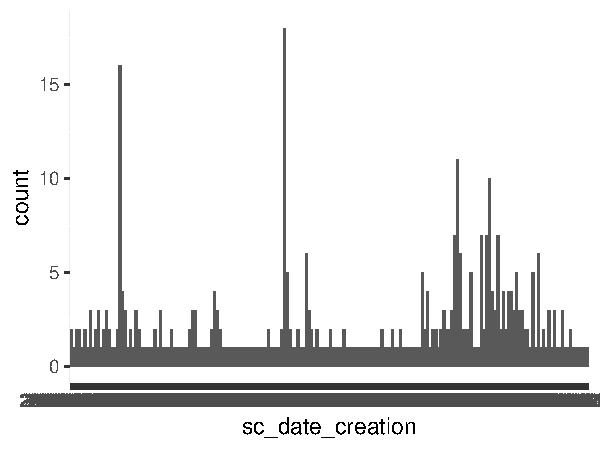
\includegraphics[keepaspectratio]{codebook_data_files/figure-pdf/Var-19-sc-date-creation-1.pdf}}

\emini

\begin{itemize}
\tightlist
\item
  Observed factor levels: ``2017-04-01'', ``2017-04-07'',
  ``2017-04-10'', ``2017-04-11'', ``2017-04-12'', ``2017-04-13'',
  ``2017-04-19'', ``2017-04-20'', ``2017-04-22'', ``2017-04-25'',
  ``2017-04-26'', ``2017-04-27'', ``2017-04-28'', ``2017-05-03'',
  ``2017-05-04'', ``2017-05-06'', ``2017-05-07'', ``2017-05-08'',
  ``2017-05-09'', ``2017-05-10'', ``2017-05-11'', ``2017-05-12'',
  ``2017-05-16'', ``2017-05-17'', ``2017-05-18'', ``2017-05-19'',
  ``2017-05-20'', ``2017-05-24'', ``2017-06-01'', ``2017-06-02'',
  ``2017-06-13'', ``2017-06-15'', ``2017-06-19'', ``2017-06-20'',
  ``2017-06-21'', ``2017-06-22'', ``2017-06-23'', ``2017-06-24'',
  ``2017-06-27'', ``2017-06-28'', ``2017-06-29'', ``2017-06-30'',
  ``2017-07-01'', ``2017-07-02'', ``2017-07-04'', ``2017-07-05'',
  ``2017-07-06'', ``2017-07-07'', ``2017-07-11'', ``2017-07-12'',
  ``2017-07-18'', ``2017-07-20'', ``2017-07-22'', ``2017-07-24'',
  ``2017-07-25'', ``2017-07-27'', ``2017-08-01'', ``2017-08-03'',
  ``2017-08-08'', ``2017-08-10'', ``2017-08-17'', ``2017-08-20'',
  ``2017-08-30'', ``2017-09-06'', ``2017-09-07'', ``2017-09-11'',
  ``2017-09-20'', ``2017-09-21'', ``2017-09-25'', ``2017-09-27'',
  ``2017-10-05'', ``2017-10-26'', ``2017-10-29'', ``2017-11-02'',
  ``2017-11-09'', ``2017-11-13'', ``2017-11-18'', ``2017-11-20'',
  ``2017-11-21'', ``2017-11-23'', ``2017-11-24'', ``2017-11-26'',
  ``2017-11-27'', ``2017-11-28'', ``2017-11-30'', ``2017-12-04'',
  ``2017-12-07'', ``2017-12-11'', ``2017-12-12'', ``2017-12-13'',
  ``2017-12-15'', ``2017-12-19'', ``2017-12-21'', ``2017-12-22'',
  ``2017-12-27'', ``2017-12-28'', ``2018-01-02'', ``2018-01-04'',
  ``2018-01-14'', ``2018-01-23'', ``2018-01-27'', ``2018-01-30'',
  ``2018-01-31'', ``2018-02-01'', ``2018-02-04'', ``2018-02-08'',
  ``2018-02-11'', ``2018-02-12'', ``2018-02-14'', ``2018-02-16'',
  ``2018-02-20'', ``2018-02-25'', ``2018-02-26'', ``2018-03-09'',
  ``2018-03-11'', ``2018-03-12'', ``2018-03-28'', ``2018-04-16'',
  ``2018-04-29'', ``2018-05-03'', ``2018-05-04'', ``2018-05-13'',
  ``2018-05-16'', ``2018-05-31'', ``2018-06-26'', ``2018-07-26'',
  ``2018-07-30'', ``2018-08-09'', ``2018-09-04'', ``2018-09-11'',
  ``2018-11-22'', ``2018-11-23'', ``2018-11-24'', ``2018-11-26'',
  ``2018-11-27'', ``2018-11-28'', ``2018-11-30'', ``2018-12-02'',
  ``2018-12-03'', ``2018-12-04'', ``2018-12-05'', ``2018-12-06'',
  ``2018-12-10'', ``2018-12-11'', ``2018-12-12'', ``2018-12-13'',
  ``2018-12-15'', ``2018-12-16'', ``2018-12-17'', ``2018-12-20'',
  ``2018-12-21'', ``2018-12-23'', ``2018-12-24'', ``2018-12-25'',
  ``2018-12-26'', ``2018-12-27'', ``2018-12-28'', ``2018-12-29'',
  ``2018-12-30'', ``2018-12-31'', ``2019-01-01'', ``2019-01-02'',
  ``2019-01-03'', ``2019-01-04'', ``2019-01-05'', ``2019-01-06'',
  ``2019-01-07'', ``2019-01-08'', ``2019-01-09'', ``2019-01-10'',
  ``2019-01-13'', ``2019-01-14'', ``2019-01-15'', ``2019-01-17'',
  ``2019-01-18'', ``2019-01-19'', ``2019-01-21'', ``2019-01-23'',
  ``2019-01-25'', ``2019-01-27'', ``2019-01-29'', ``2019-01-30'',
  ``2019-02-01'', ``2019-02-03'', ``2019-02-14'', ``2019-02-17'',
  ``2019-02-18'', ``2019-02-26'', ``2019-02-27'', ``2019-03-03'',
  ``2019-03-12'', ``2019-04-29''.
\end{itemize}

\fullline

\subsection{sc\_an\_diplome}\label{sc_an_diplome}

\bminione

\begin{longtable}[]{@{}lr@{}}
\toprule\noalign{}
Feature & Result \\
\midrule\noalign{}
\endhead
\bottomrule\noalign{}
\endlastfoot
Variable type & integer \\
Number of missing obs. & 89 (19.6 \%) \\
Number of unique values & 39 \\
Median & 2010 \\
1st and 3rd quartiles & 2002; 2015 \\
Min. and max. & 1961; 2018 \\
\end{longtable}

\emini
\bminitwo

\pandocbounded{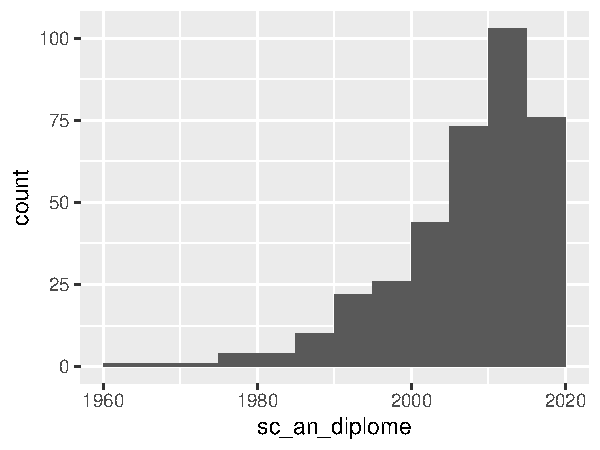
\includegraphics[keepaspectratio]{codebook_data_files/figure-pdf/Var-20-sc-an-diplome-1.pdf}}

\emini

\fullline

\subsection{sc\_diplome}\label{sc_diplome}

\bminione

\begin{longtable}[]{@{}lr@{}}
\toprule\noalign{}
Feature & Result \\
\midrule\noalign{}
\endhead
\bottomrule\noalign{}
\endlastfoot
Variable type & integer \\
Number of missing obs. & 69 (15.2 \%) \\
Number of unique values & 9 \\
Median & 6 \\
1st and 3rd quartiles & 4; 8 \\
Min. and max. & 1; 999 \\
\end{longtable}

\emini
\bminitwo

\pandocbounded{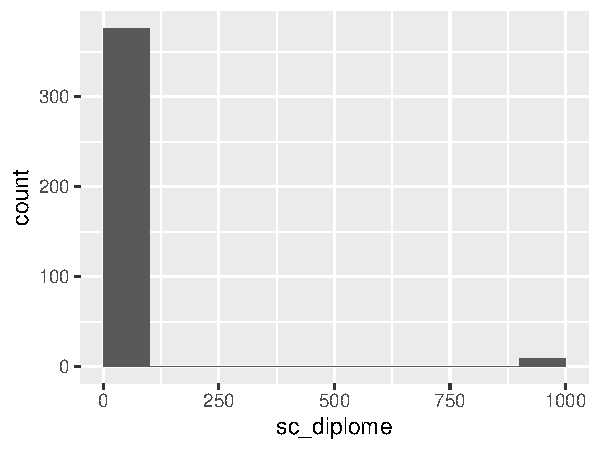
\includegraphics[keepaspectratio]{codebook_data_files/figure-pdf/Var-21-sc-diplome-1.pdf}}

\emini

\fullline

\subsection{sc\_diplome\_autre}\label{sc_diplome_autre}

\bminione

\begin{longtable}[]{@{}lr@{}}
\toprule\noalign{}
Feature & Result \\
\midrule\noalign{}
\endhead
\bottomrule\noalign{}
\endlastfoot
Variable type & character \\
Number of missing obs. & 445 (98.02 \%) \\
Number of unique values & 9 \\
Mode & ``Bac + 6'' \\
\end{longtable}

\emini
\bminitwo

\pandocbounded{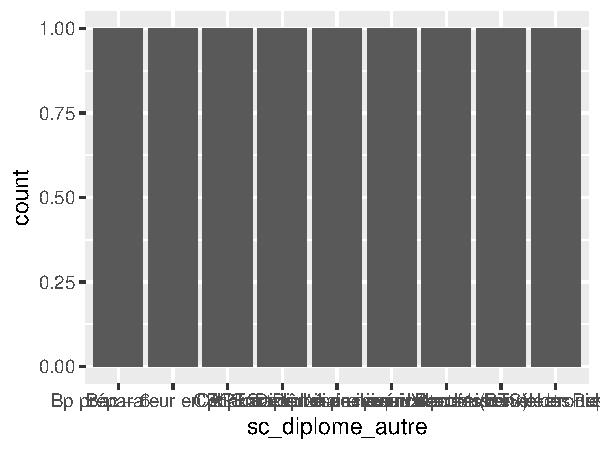
\includegraphics[keepaspectratio]{codebook_data_files/figure-pdf/Var-22-sc-diplome-autre-1.pdf}}

\emini

\begin{itemize}
\tightlist
\item
  Observed factor levels: ``Bac + 6'', ``Bp préparateur en pharmacie'',
  ``CAPES'', ``CESS art de l'espace'', ``diplome auxiliaire
  puériculture'', ``Diplômé de niveau Bac +1 (BTS)'', ``Diplome niveau
  IV technicien électronique'', ``equivalent au brevet des collége'',
  ``Licence professionnel en Ressources Humaine''.
\end{itemize}

\fullline

\subsection{sc\_fin\_etudes}\label{sc_fin_etudes}

\bminione

\begin{longtable}[]{@{}lr@{}}
\toprule\noalign{}
Feature & Result \\
\midrule\noalign{}
\endhead
\bottomrule\noalign{}
\endlastfoot
Variable type & integer \\
Number of missing obs. & 64 (14.1 \%) \\
Number of unique values & 2 \\
Median & 1 \\
1st and 3rd quartiles & 1; 1 \\
Min. and max. & 0; 1 \\
\end{longtable}

\emini
\bminitwo

\pandocbounded{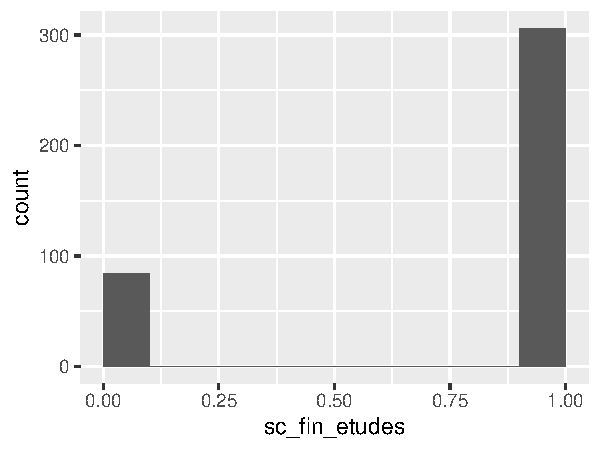
\includegraphics[keepaspectratio]{codebook_data_files/figure-pdf/Var-23-sc-fin-etudes-1.pdf}}

\emini

\fullline

\subsection{sc\_formation}\label{sc_formation}

\bminione

\begin{longtable}[]{@{}lr@{}}
\toprule\noalign{}
Feature & Result \\
\midrule\noalign{}
\endhead
\bottomrule\noalign{}
\endlastfoot
Variable type & integer \\
Number of missing obs. & 371 (81.72 \%) \\
Number of unique values & 18 \\
Median & 20 \\
1st and 3rd quartiles & 14; 24 \\
Min. and max. & 8; 999 \\
\end{longtable}

\emini
\bminitwo

\pandocbounded{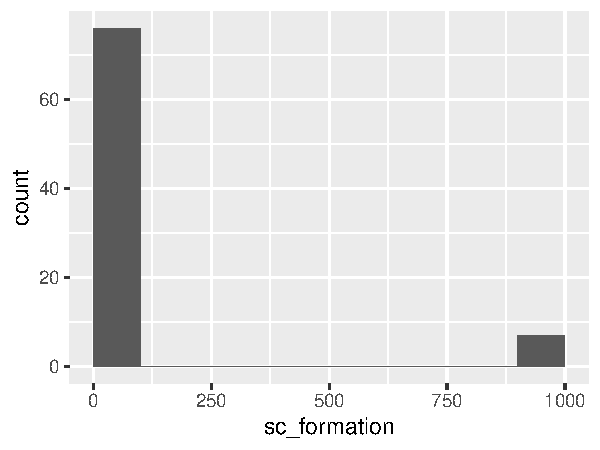
\includegraphics[keepaspectratio]{codebook_data_files/figure-pdf/Var-24-sc-formation-1.pdf}}

\emini

\fullline

\subsection{sc\_formation\_autre}\label{sc_formation_autre}

\bminione

\begin{longtable}[]{@{}lr@{}}
\toprule\noalign{}
Feature & Result \\
\midrule\noalign{}
\endhead
\bottomrule\noalign{}
\endlastfoot
Variable type & character \\
Number of missing obs. & 447 (98.46 \%) \\
Number of unique values & 7 \\
Mode & ``9eme année de médecine'' \\
\end{longtable}

\emini
\bminitwo

\pandocbounded{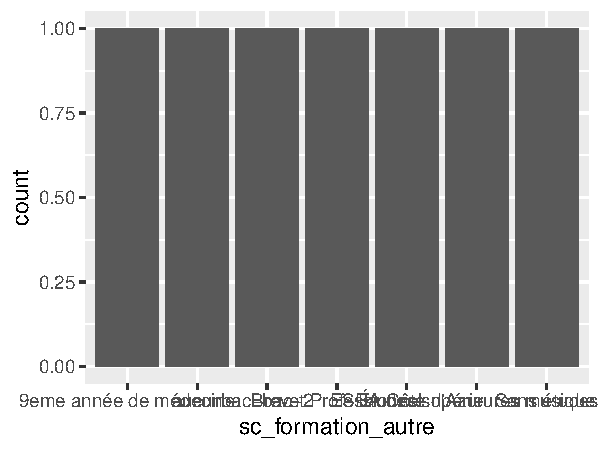
\includegraphics[keepaspectratio]{codebook_data_files/figure-pdf/Var-25-sc-formation-autre-1.pdf}}

\emini

\begin{itemize}
\tightlist
\item
  Observed factor levels: ``9eme année de médecine'', ``aucun'',
  ``bac-bac+2'', ``Brevet Professionnel'', ``ESRA Côte d'Azur'',
  ``Études supérieures musique'', ``Sans études''.
\end{itemize}

\fullline

\subsection{sc\_plan}\label{sc_plan}

\bminione

\begin{longtable}[]{@{}lr@{}}
\toprule\noalign{}
Feature & Result \\
\midrule\noalign{}
\endhead
\bottomrule\noalign{}
\endlastfoot
Variable type & integer \\
Number of missing obs. & 68 (14.98 \%) \\
Number of unique values & 2 \\
Median & 0 \\
1st and 3rd quartiles & 0; 0 \\
Min. and max. & 0; 1 \\
\end{longtable}

\emini
\bminitwo

\pandocbounded{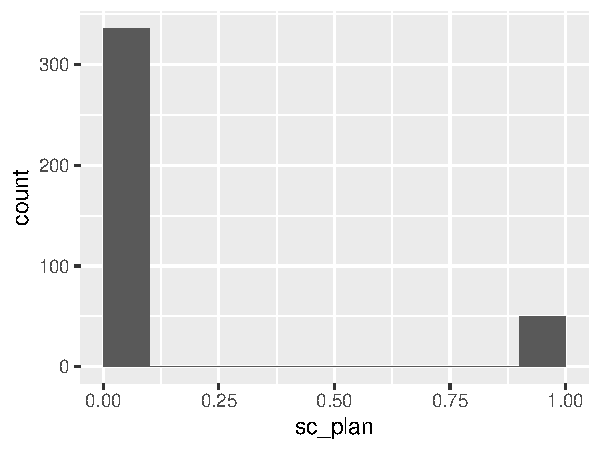
\includegraphics[keepaspectratio]{codebook_data_files/figure-pdf/Var-26-sc-plan-1.pdf}}

\emini

\fullline

\subsection{sc\_plan\_an}\label{sc_plan_an}

\bminione

\begin{longtable}[]{@{}lr@{}}
\toprule\noalign{}
Feature & Result \\
\midrule\noalign{}
\endhead
\bottomrule\noalign{}
\endlastfoot
Variable type & integer \\
Number of missing obs. & 428 (94.27 \%) \\
Number of unique values & 15 \\
Median & 2003 \\
1st and 3rd quartiles & 1999.5; 2005 \\
Min. and max. & 1988; 2011 \\
\end{longtable}

\emini
\bminitwo

\pandocbounded{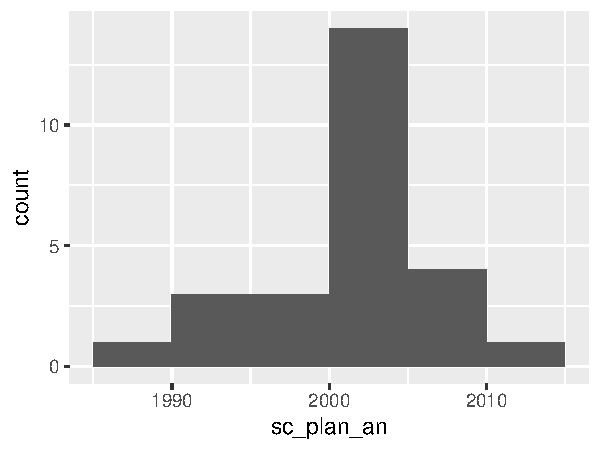
\includegraphics[keepaspectratio]{codebook_data_files/figure-pdf/Var-27-sc-plan-an-1.pdf}}

\emini

\fullline

\subsection{sc\_plan\_demande}\label{sc_plan_demande}

\bminione

\begin{longtable}[]{@{}lr@{}}
\toprule\noalign{}
Feature & Result \\
\midrule\noalign{}
\endhead
\bottomrule\noalign{}
\endlastfoot
Variable type & integer \\
Number of missing obs. & 139 (30.62 \%) \\
Number of unique values & 2 \\
Median & 0 \\
1st and 3rd quartiles & 0; 0 \\
Min. and max. & 0; 1 \\
\end{longtable}

\emini
\bminitwo

\pandocbounded{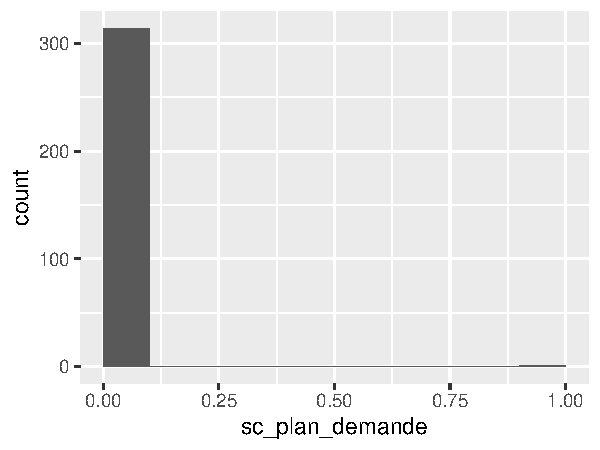
\includegraphics[keepaspectratio]{codebook_data_files/figure-pdf/Var-28-sc-plan-demande-1.pdf}}

\emini

\fullline

\subsection{sc\_plan\_ets1\_1}\label{sc_plan_ets1_1}

\begin{itemize}
\tightlist
\item
  The variable only takes one (non-missing) value: ``1''. The variable
  contains 94.05 \% missing observations.
\end{itemize}

\fullline

\subsection{sc\_plan\_ets1\_2}\label{sc_plan_ets1_2}

\begin{itemize}
\tightlist
\item
  The variable only takes one (non-missing) value: ``1''. The variable
  contains 94.27 \% missing observations.
\end{itemize}

\fullline

\subsection{sc\_plan\_ets1\_3}\label{sc_plan_ets1_3}

\begin{itemize}
\tightlist
\item
  The variable only takes one (non-missing) value: ``1''. The variable
  contains 94.27 \% missing observations.
\end{itemize}

\fullline

\subsection{sc\_plan\_ets1\_4}\label{sc_plan_ets1_4}

\begin{itemize}
\tightlist
\item
  The variable only takes one (non-missing) value: ``1''. The variable
  contains 94.05 \% missing observations.
\end{itemize}

\fullline

\subsection{sc\_plan\_ets1\_5}\label{sc_plan_ets1_5}

\begin{itemize}
\tightlist
\item
  The variable only takes one (non-missing) value: ``1''. The variable
  contains 94.05 \% missing observations.
\end{itemize}

\fullline

\subsection{sc\_plan\_ets1\_6}\label{sc_plan_ets1_6}

\begin{itemize}
\tightlist
\item
  The variable only takes one (non-missing) value: ``1''. The variable
  contains 92.51 \% missing observations.
\end{itemize}

\fullline

\subsection{sc\_plan\_ets1\_7}\label{sc_plan_ets1_7}

\begin{itemize}
\tightlist
\item
  The variable only takes one (non-missing) value: ``1''. The variable
  contains 92.29 \% missing observations.
\end{itemize}

\fullline

\subsection{sc\_plan\_ets1\_8}\label{sc_plan_ets1_8}

\begin{itemize}
\tightlist
\item
  The variable only takes one (non-missing) value: ``1''. The variable
  contains 92.51 \% missing observations.
\end{itemize}

\fullline

\subsection{sc\_plan\_ets1\_9}\label{sc_plan_ets1_9}

\begin{itemize}
\tightlist
\item
  The variable only takes one (non-missing) value: ``1''. The variable
  contains 92.29 \% missing observations.
\end{itemize}

\fullline

\subsection{sc\_plan\_ets1\_12}\label{sc_plan_ets1_12}

\begin{itemize}
\tightlist
\item
  The variable only takes one (non-missing) value: ``1''. The variable
  contains 92.73 \% missing observations.
\end{itemize}

\fullline

\subsection{sc\_plan\_ets1\_13}\label{sc_plan_ets1_13}

\begin{itemize}
\tightlist
\item
  The variable only takes one (non-missing) value: ``1''. The variable
  contains 92.73 \% missing observations.
\end{itemize}

\fullline

\subsection{sc\_plan\_ets1\_14}\label{sc_plan_ets1_14}

\begin{itemize}
\tightlist
\item
  The variable only takes one (non-missing) value: ``1''. The variable
  contains 92.73 \% missing observations.
\end{itemize}

\fullline

\subsection{sc\_plan\_ets2\_1}\label{sc_plan_ets2_1}

\begin{itemize}
\tightlist
\item
  The variable only takes one (non-missing) value: ``1''. The variable
  contains 99.78 \% missing observations.
\end{itemize}

\fullline

\subsection{sc\_plan\_ets2\_2}\label{sc_plan_ets2_2}

\begin{itemize}
\tightlist
\item
  The variable only takes one (non-missing) value: ``1''. The variable
  contains 99.34 \% missing observations.
\end{itemize}

\fullline

\subsection{sc\_plan\_ets2\_3}\label{sc_plan_ets2_3}

\begin{itemize}
\tightlist
\item
  The variable only takes one (non-missing) value: ``1''. The variable
  contains 99.34 \% missing observations.
\end{itemize}

\fullline

\subsection{sc\_plan\_ets2\_4}\label{sc_plan_ets2_4}

\begin{itemize}
\tightlist
\item
  The variable only takes one (non-missing) value: ``1''. The variable
  contains 99.34 \% missing observations.
\end{itemize}

\fullline

\subsection{sc\_plan\_ets2\_5}\label{sc_plan_ets2_5}

\begin{itemize}
\tightlist
\item
  The variable only takes one (non-missing) value: ``1''. The variable
  contains 99.56 \% missing observations.
\end{itemize}

\fullline

\subsection{sc\_plan\_ets2\_6}\label{sc_plan_ets2_6}

\begin{itemize}
\tightlist
\item
  The variable only takes one (non-missing) value: ``1''. The variable
  contains 99.56 \% missing observations.
\end{itemize}

\fullline

\subsection{sc\_plan\_ets2\_7}\label{sc_plan_ets2_7}

\begin{itemize}
\tightlist
\item
  The variable only takes one (non-missing) value: ``1''. The variable
  contains 99.56 \% missing observations.
\end{itemize}

\fullline

\subsection{sc\_plan\_ets2\_8}\label{sc_plan_ets2_8}

\begin{itemize}
\tightlist
\item
  The variable only takes one (non-missing) value: ``1''. The variable
  contains 99.56 \% missing observations.
\end{itemize}

\fullline

\subsection{sc\_plan\_ets2\_9}\label{sc_plan_ets2_9}

\begin{itemize}
\tightlist
\item
  The variable only takes one (non-missing) value: ``1''. The variable
  contains 99.78 \% missing observations.
\end{itemize}

\fullline

\subsection{sc\_plan\_ets2\_14}\label{sc_plan_ets2_14}

\begin{itemize}
\tightlist
\item
  The variable only takes one (non-missing) value: ``1''. The variable
  contains 99.78 \% missing observations.
\end{itemize}

\fullline

\subsection{sc\_plan\_ets5\_13}\label{sc_plan_ets5_13}

\begin{itemize}
\tightlist
\item
  The variable only takes one (non-missing) value: ``1''. The variable
  contains 99.56 \% missing observations.
\end{itemize}

\fullline

\subsection{sc\_plan\_ets5\_14}\label{sc_plan_ets5_14}

\begin{itemize}
\tightlist
\item
  The variable only takes one (non-missing) value: ``1''. The variable
  contains 99.56 \% missing observations.
\end{itemize}

\fullline

\subsection{sc\_plan\_notification\_1}\label{sc_plan_notification_1}

\begin{itemize}
\tightlist
\item
  The variable only takes one (non-missing) value: ``1''. The variable
  contains 99.78 \% missing observations.
\end{itemize}

\fullline

\subsection{sc\_plan\_notification\_2}\label{sc_plan_notification_2}

\begin{itemize}
\tightlist
\item
  The variable only takes one (non-missing) value: ``1''. The variable
  contains 99.34 \% missing observations.
\end{itemize}

\fullline

\subsection{sc\_plan\_notification\_3}\label{sc_plan_notification_3}

\begin{itemize}
\tightlist
\item
  The variable only takes one (non-missing) value: ``1''. The variable
  contains 99.56 \% missing observations.
\end{itemize}

\fullline

\subsection{sc\_plan\_notification\_4}\label{sc_plan_notification_4}

\begin{itemize}
\tightlist
\item
  The variable only takes one (non-missing) value: ``1''. The variable
  contains 99.78 \% missing observations.
\end{itemize}

\fullline

\subsection{sc\_plan\_notification\_5}\label{sc_plan_notification_5}

\begin{itemize}
\tightlist
\item
  The variable only takes one (non-missing) value: ``1''. The variable
  contains 99.56 \% missing observations.
\end{itemize}

\fullline

\subsection{sc\_plan\_notification\_6}\label{sc_plan_notification_6}

\begin{itemize}
\tightlist
\item
  The variable only takes one (non-missing) value: ``1''. The variable
  contains 97.36 \% missing observations.
\end{itemize}

\fullline

\subsection{sc\_plan\_notification\_7}\label{sc_plan_notification_7}

\begin{itemize}
\tightlist
\item
  The variable only takes one (non-missing) value: ``1''. The variable
  contains 98.9 \% missing observations.
\end{itemize}

\fullline

\subsection{sc\_plan\_notification\_8}\label{sc_plan_notification_8}

\begin{itemize}
\tightlist
\item
  The variable only takes one (non-missing) value: ``1''. The variable
  contains 98.24 \% missing observations.
\end{itemize}

\fullline

\subsection{sc\_plan\_notification\_999}\label{sc_plan_notification_999}

\begin{itemize}
\tightlist
\item
  The variable only takes one (non-missing) value: ``1''. The variable
  contains 96.7 \% missing observations.
\end{itemize}

\fullline

\subsection{sc\_plan\_notification\_autre}\label{sc_plan_notification_autre}

\bminione

\begin{longtable}[]{@{}lr@{}}
\toprule\noalign{}
Feature & Result \\
\midrule\noalign{}
\endhead
\bottomrule\noalign{}
\endlastfoot
Variable type & character \\
Number of missing obs. & 439 (96.7 \%) \\
Number of unique values & 15 \\
Mode & ``1/3 temps pour les épreuves'' \\
\end{longtable}

\emini
\bminitwo

\pandocbounded{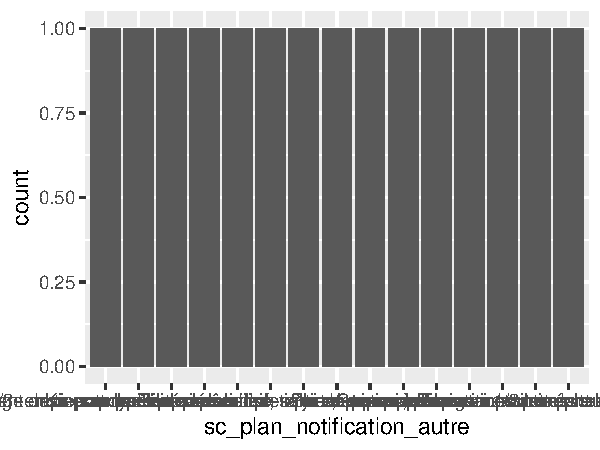
\includegraphics[keepaspectratio]{codebook_data_files/figure-pdf/Var-62-sc-plan-notification-autre-1.pdf}}

\emini

\begin{itemize}
\tightlist
\item
  Observed factor levels: ``1/3 temps pour les épreuves'', ``Adaptation
  des horaires de classe, rattrapage des cours par les camarades, tiers
  temps supplémentaires aux épreuves'', ``Aménagement du tiers temps
  supplémentaires pour les examens'', ``Ecole spécialisé'', ``Kine au
  lycée mais là mdph n?y est pour rien!!'', ``non port des livres
  scolaires, salle de repos à disposition'', ``Pai'', ``possibilité de
  sortir de cours, et pour les exams 1/3 temps'', ``rien'', ``Soutien
  scolaire'', ``Taxi'', ``tiers temps'', ``tiers-temps, pause aux
  toilettes lors d'examens'', ``un aménagement pendant les examens'',
  ``un tiers-temps''.
\end{itemize}

\fullline

\subsection{sc\_an\_debut}\label{sc_an_debut}

\bminione

\begin{longtable}[]{@{}lr@{}}
\toprule\noalign{}
Feature & Result \\
\midrule\noalign{}
\endhead
\bottomrule\noalign{}
\endlastfoot
Variable type & integer \\
Number of missing obs. & 0 (0 \%) \\
Number of unique values & 52 \\
Median & 1993 \\
1st and 3rd quartiles & 1986; 1999 \\
Min. and max. & 1950; 2010 \\
\end{longtable}

\emini
\bminitwo

\pandocbounded{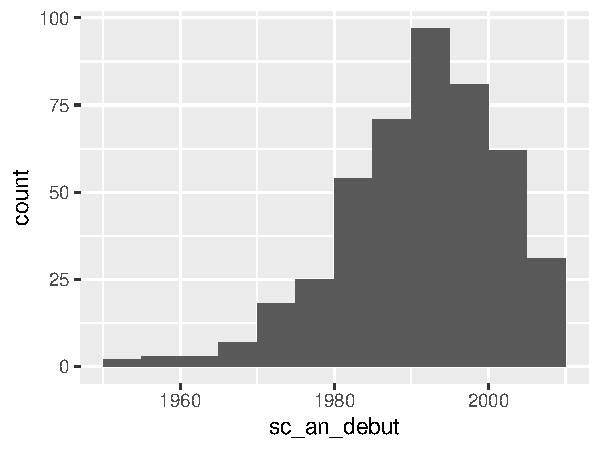
\includegraphics[keepaspectratio]{codebook_data_files/figure-pdf/Var-63-sc-an-debut-1.pdf}}

\emini

\fullline

\subsection{sc\_debut}\label{sc_debut}

\bminione

\begin{longtable}[]{@{}lr@{}}
\toprule\noalign{}
Feature & Result \\
\midrule\noalign{}
\endhead
\bottomrule\noalign{}
\endlastfoot
Variable type & integer \\
Number of missing obs. & 0 (0 \%) \\
Number of unique values & 3 \\
Median & 1 \\
1st and 3rd quartiles & 1; 1 \\
Min. and max. & 1; 999 \\
\end{longtable}

\emini
\bminitwo

\pandocbounded{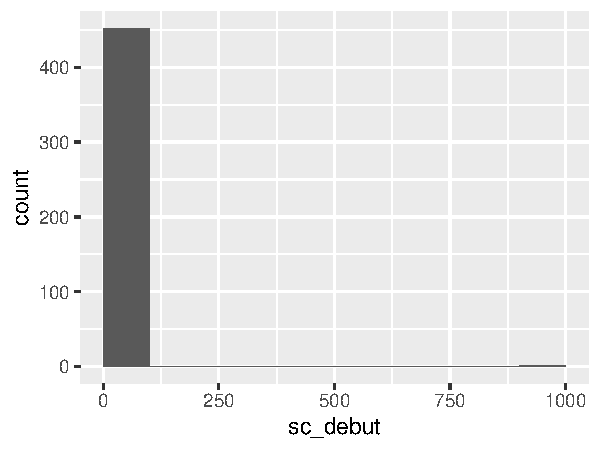
\includegraphics[keepaspectratio]{codebook_data_files/figure-pdf/Var-64-sc-debut-1.pdf}}

\emini

\fullline

\subsection{sc\_debut\_autre}\label{sc_debut_autre}

\bminione

\begin{longtable}[]{@{}lr@{}}
\toprule\noalign{}
Feature & Result \\
\midrule\noalign{}
\endhead
\bottomrule\noalign{}
\endlastfoot
Variable type & character \\
Number of missing obs. & 452 (99.56 \%) \\
Number of unique values & 2 \\
Mode & ``1 ere primaire (belgique)'' \\
\end{longtable}

\emini
\bminitwo

\pandocbounded{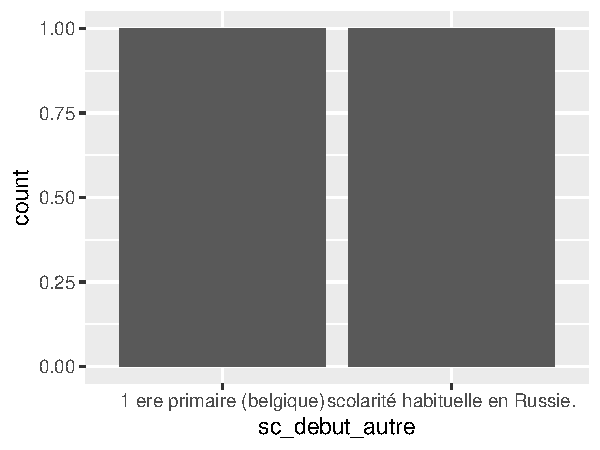
\includegraphics[keepaspectratio]{codebook_data_files/figure-pdf/Var-65-sc-debut-autre-1.pdf}}

\emini

\begin{itemize}
\tightlist
\item
  Observed factor levels: ``1 ere primaire (belgique)'', ``scolarité
  habituelle en Russie.''.
\end{itemize}

\fullline

\subsection{sc\_interromp}\label{sc_interromp}

\bminione

\begin{longtable}[]{@{}lr@{}}
\toprule\noalign{}
Feature & Result \\
\midrule\noalign{}
\endhead
\bottomrule\noalign{}
\endlastfoot
Variable type & integer \\
Number of missing obs. & 64 (14.1 \%) \\
Number of unique values & 2 \\
Median & 0 \\
1st and 3rd quartiles & 0; 1 \\
Min. and max. & 0; 1 \\
\end{longtable}

\emini
\bminitwo

\pandocbounded{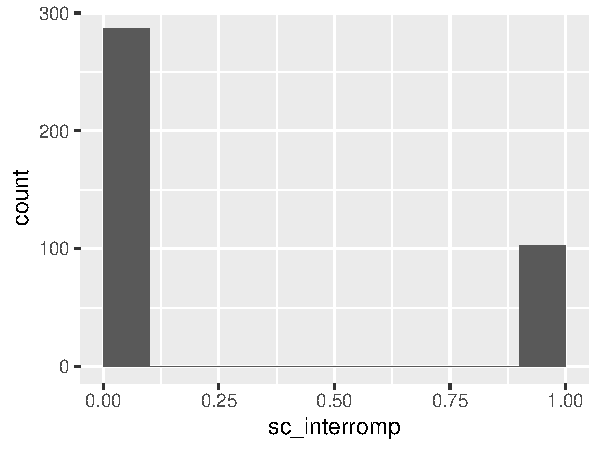
\includegraphics[keepaspectratio]{codebook_data_files/figure-pdf/Var-66-sc-interromp-1.pdf}}

\emini

\fullline

\subsection{sc\_redoubl}\label{sc_redoubl}

\bminione

\begin{longtable}[]{@{}lr@{}}
\toprule\noalign{}
Feature & Result \\
\midrule\noalign{}
\endhead
\bottomrule\noalign{}
\endlastfoot
Variable type & integer \\
Number of missing obs. & 54 (11.89 \%) \\
Number of unique values & 2 \\
Median & 0 \\
1st and 3rd quartiles & 0; 1 \\
Min. and max. & 0; 1 \\
\end{longtable}

\emini
\bminitwo

\pandocbounded{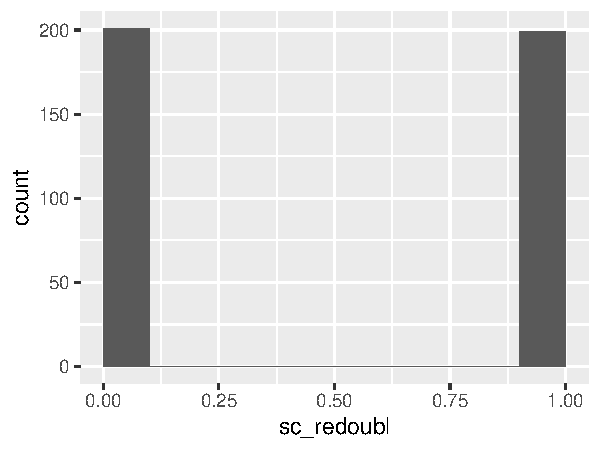
\includegraphics[keepaspectratio]{codebook_data_files/figure-pdf/Var-67-sc-redoubl-1.pdf}}

\emini

\fullline

\subsection{sc\_type}\label{sc_type}

\begin{itemize}
\tightlist
\item
  The variable only takes one (non-missing) value: ``P''. The variable
  contains 11.23 \% missing observations.
\end{itemize}

\fullline

\subsection{id\_sc\_cat}\label{id_sc_cat}

\bminione

\begin{longtable}[]{@{}lr@{}}
\toprule\noalign{}
Feature & Result \\
\midrule\noalign{}
\endhead
\bottomrule\noalign{}
\endlastfoot
Variable type & character \\
Number of missing obs. & 0 (0 \%) \\
Number of unique values & 2 \\
Mode & ``id\_01\_sc\_02'' \\
\end{longtable}

\emini
\bminitwo

\pandocbounded{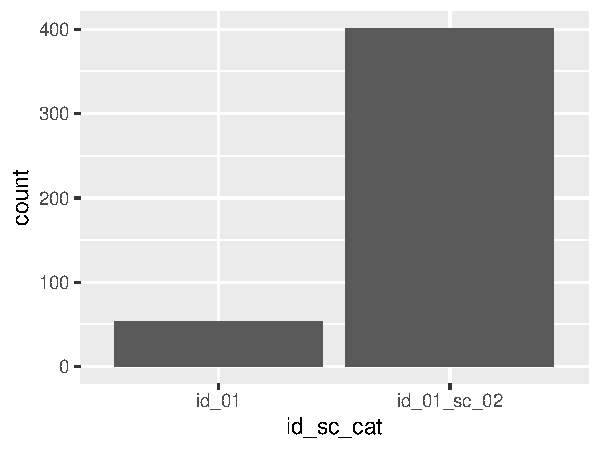
\includegraphics[keepaspectratio]{codebook_data_files/figure-pdf/Var-69-id-sc-cat-1.pdf}}

\emini

\begin{itemize}
\tightlist
\item
  Observed factor levels: ``id\_01'', ``id\_01\_sc\_02''.
\end{itemize}

\fullline

\subsection{id\_age\_cat\_2}\label{id_age_cat_2}

\bminione

\begin{longtable}[]{@{}lr@{}}
\toprule\noalign{}
Feature & Result \\
\midrule\noalign{}
\endhead
\bottomrule\noalign{}
\endlastfoot
Variable type & character \\
Number of missing obs. & 0 (0 \%) \\
Number of unique values & 2 \\
Mode & ``Adulte'' \\
\end{longtable}

\emini
\bminitwo

\pandocbounded{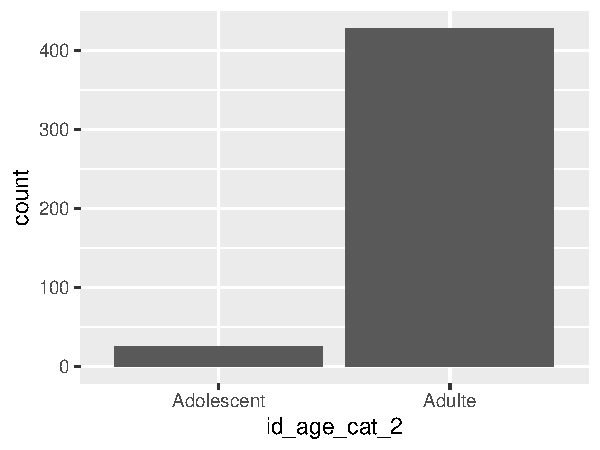
\includegraphics[keepaspectratio]{codebook_data_files/figure-pdf/Var-70-id-age-cat-2-1.pdf}}

\emini

\begin{itemize}
\tightlist
\item
  Observed factor levels: ``Adolescent'', ``Adulte''.
\end{itemize}

\fullline

\subsection{id\_age\_cat\_3}\label{id_age_cat_3}

\bminione

\begin{longtable}[]{@{}lr@{}}
\toprule\noalign{}
Feature & Result \\
\midrule\noalign{}
\endhead
\bottomrule\noalign{}
\endlastfoot
Variable type & character \\
Number of missing obs. & 26 (5.73 \%) \\
Number of unique values & 3 \\
Mode & ``18-29 ans'' \\
\end{longtable}

\emini
\bminitwo

\pandocbounded{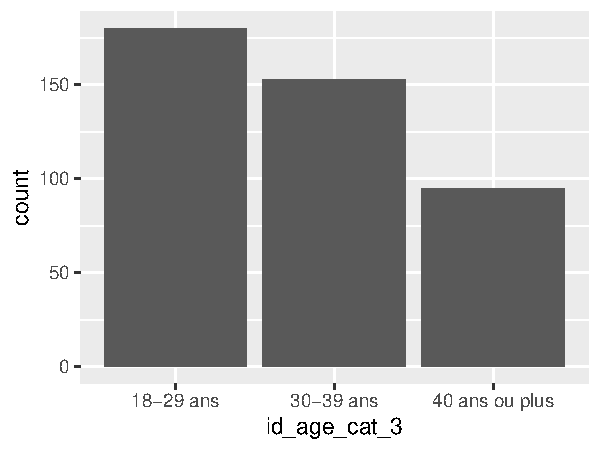
\includegraphics[keepaspectratio]{codebook_data_files/figure-pdf/Var-71-id-age-cat-3-1.pdf}}

\emini

\begin{itemize}
\tightlist
\item
  Observed factor levels: ``18-29 ans'', ``30-39 ans'', ``40 ans ou
  plus''.
\end{itemize}

\fullline

\subsection{sc\_debut\_corr}\label{sc_debut_corr}

\begin{itemize}
\tightlist
\item
  The variable only takes one (non-missing) value: ``1''. The variable
  contains 65.86 \% missing observations.
\end{itemize}

\fullline

\subsection{sc\_date\_debut}\label{sc_date_debut}

\bminione

\begin{longtable}[]{@{}lr@{}}
\toprule\noalign{}
Feature & Result \\
\midrule\noalign{}
\endhead
\bottomrule\noalign{}
\endlastfoot
Variable type & character \\
Number of missing obs. & 0 (0 \%) \\
Number of unique values & 52 \\
Mode & ``1996-09-01'' \\
\end{longtable}

\emini
\bminitwo

\pandocbounded{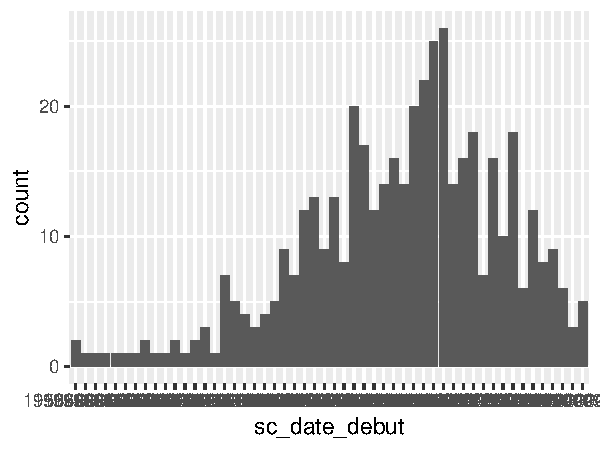
\includegraphics[keepaspectratio]{codebook_data_files/figure-pdf/Var-73-sc-date-debut-1.pdf}}

\emini

\begin{itemize}
\tightlist
\item
  Observed factor levels: ``1950-09-01'', ``1956-09-01'',
  ``1959-09-01'', ``1960-09-01'', ``1963-09-01'', ``1964-09-01'',
  ``1965-09-01'', ``1966-09-01'', ``1967-09-01'', ``1968-09-01'',
  ``1969-09-01'', ``1970-09-01'', ``1971-09-01'', ``1972-09-01'',
  ``1973-09-01'', ``1974-09-01'', ``1975-09-01'', ``1976-09-01'',
  ``1977-09-01'', ``1978-09-01'', ``1979-09-01'', ``1980-09-01'',
  ``1981-09-01'', ``1982-09-01'', ``1983-09-01'', ``1984-09-01'',
  ``1985-09-01'', ``1986-09-01'', ``1987-09-01'', ``1988-09-01'',
  ``1989-09-01'', ``1990-09-01'', ``1991-09-01'', ``1992-09-01'',
  ``1993-09-01'', ``1994-09-01'', ``1995-09-01'', ``1996-09-01'',
  ``1997-09-01'', ``1998-09-01'', ``1999-09-01'', ``2000-09-01'',
  ``2001-09-01'', ``2002-09-01'', ``2003-09-01'', ``2004-09-01'',
  ``2005-09-01'', ``2006-09-01'', ``2007-09-01'', ``2008-09-01'',
  ``2009-09-01'', ``2010-09-01''.
\end{itemize}

\fullline

\subsection{sc\_age\_debut}\label{sc_age_debut}

\bminione

\begin{longtable}[]{@{}lr@{}}
\toprule\noalign{}
Feature & Result \\
\midrule\noalign{}
\endhead
\bottomrule\noalign{}
\endlastfoot
Variable type & integer \\
Number of missing obs. & 2 (0.44 \%) \\
Number of unique values & 3 \\
Median & 6 \\
1st and 3rd quartiles & 6; 6 \\
Min. and max. & 5; 7 \\
\end{longtable}

\emini
\bminitwo

\pandocbounded{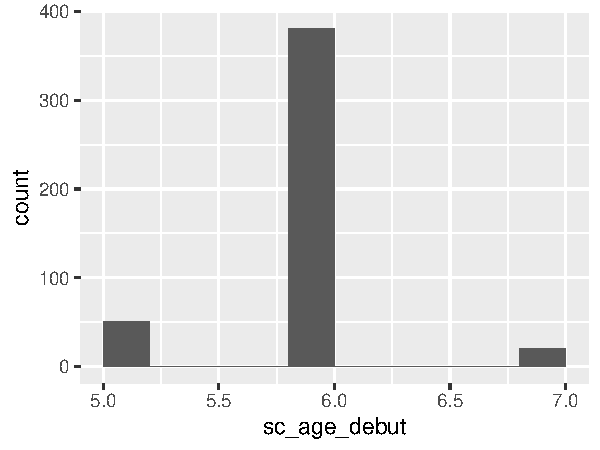
\includegraphics[keepaspectratio]{codebook_data_files/figure-pdf/Var-74-sc-age-debut-1.pdf}}

\emini

\fullline

\subsection{sc\_etspps}\label{sc_etspps}

\bminione

\begin{longtable}[]{@{}lr@{}}
\toprule\noalign{}
Feature & Result \\
\midrule\noalign{}
\endhead
\bottomrule\noalign{}
\endlastfoot
Variable type & character \\
Number of missing obs. & 405 (89.21 \%) \\
Number of unique values & 3 \\
Mode & ``1-Classe ordinaire'' \\
\end{longtable}

\emini
\bminitwo

\pandocbounded{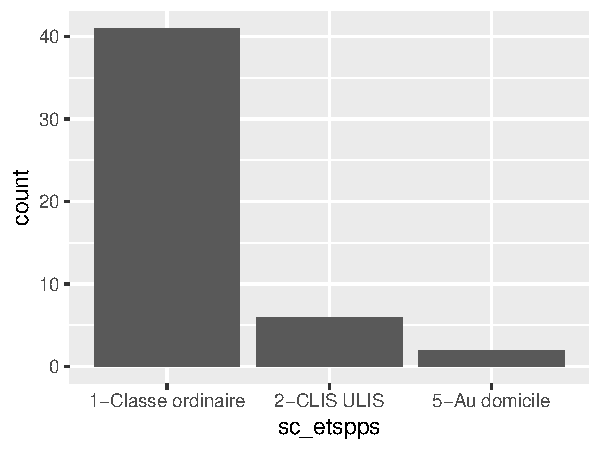
\includegraphics[keepaspectratio]{codebook_data_files/figure-pdf/Var-75-sc-etspps-1.pdf}}

\emini

\begin{itemize}
\tightlist
\item
  Observed factor levels: ``1-Classe ordinaire'', ``2-CLIS ULIS'',
  ``5-Au domicile''.
\end{itemize}

\fullline

\subsection{sc\_diplome\_cat}\label{sc_diplome_cat}

\bminione

\begin{longtable}[]{@{}lr@{}}
\toprule\noalign{}
Feature & Result \\
\midrule\noalign{}
\endhead
\bottomrule\noalign{}
\endlastfoot
Variable type & character \\
Number of missing obs. & 78 (17.18 \%) \\
Number of unique values & 5 \\
Mode & ``5-Diplôme du supérieur long (bac+3,4,5)'' \\
\end{longtable}

\emini
\bminitwo

\pandocbounded{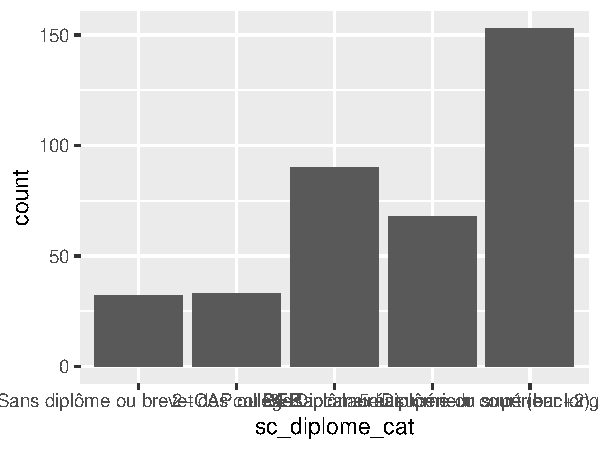
\includegraphics[keepaspectratio]{codebook_data_files/figure-pdf/Var-76-sc-diplome-cat-1.pdf}}

\emini

\begin{itemize}
\tightlist
\item
  Observed factor levels: ``1-Sans diplôme ou brevet des collèges'',
  ``2-CAP ou BEP'', ``3-Baccalauréat'', ``4-Diplôme du supérieur court
  (bac+2)'', ``5-Diplôme du supérieur long (bac+3,4,5)''.
\end{itemize}

\fullline

\subsection{sc\_date\_diplome}\label{sc_date_diplome}

\bminione

\begin{longtable}[]{@{}lr@{}}
\toprule\noalign{}
Feature & Result \\
\midrule\noalign{}
\endhead
\bottomrule\noalign{}
\endlastfoot
Variable type & character \\
Number of missing obs. & 89 (19.6 \%) \\
Number of unique values & 39 \\
Mode & ``2016-06-30'' \\
\end{longtable}

\emini
\bminitwo

\pandocbounded{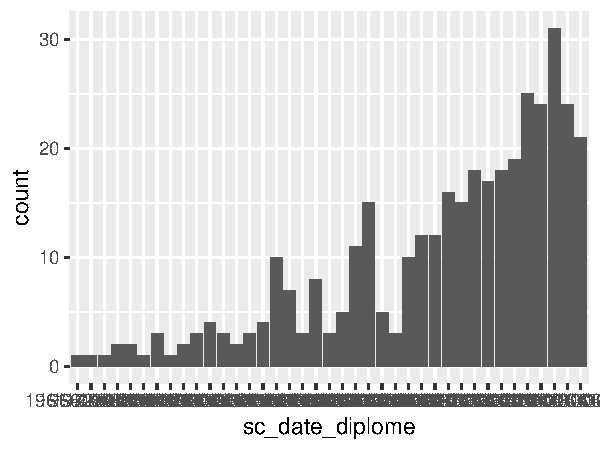
\includegraphics[keepaspectratio]{codebook_data_files/figure-pdf/Var-77-sc-date-diplome-1.pdf}}

\emini

\begin{itemize}
\tightlist
\item
  Observed factor levels: ``1961-06-30'', ``1966-06-30'',
  ``1972-06-30'', ``1978-06-30'', ``1980-06-30'', ``1983-06-30'',
  ``1985-06-30'', ``1986-06-30'', ``1987-06-30'', ``1988-06-30'',
  ``1990-06-30'', ``1991-06-30'', ``1992-06-30'', ``1993-06-30'',
  ``1994-06-30'', ``1995-06-30'', ``1996-06-30'', ``1997-06-30'',
  ``1998-06-30'', ``1999-06-30'', ``2000-06-30'', ``2001-06-30'',
  ``2002-06-30'', ``2003-06-30'', ``2004-06-30'', ``2005-06-30'',
  ``2006-06-30'', ``2007-06-30'', ``2008-06-30'', ``2009-06-30'',
  ``2010-06-30'', ``2011-06-30'', ``2012-06-30'', ``2013-06-30'',
  ``2014-06-30'', ``2015-06-30'', ``2016-06-30'', ``2017-06-30'',
  ``2018-06-30''.
\end{itemize}

\fullline

\subsection{sc\_age\_diplome}\label{sc_age_diplome}

\bminione

\begin{longtable}[]{@{}lr@{}}
\toprule\noalign{}
Feature & Result \\
\midrule\noalign{}
\endhead
\bottomrule\noalign{}
\endlastfoot
Variable type & integer \\
Number of missing obs. & 91 (20.04 \%) \\
Number of unique values & 24 \\
Median & 22 \\
1st and 3rd quartiles & 19; 24 \\
Min. and max. & 13; 38 \\
\end{longtable}

\emini
\bminitwo

\pandocbounded{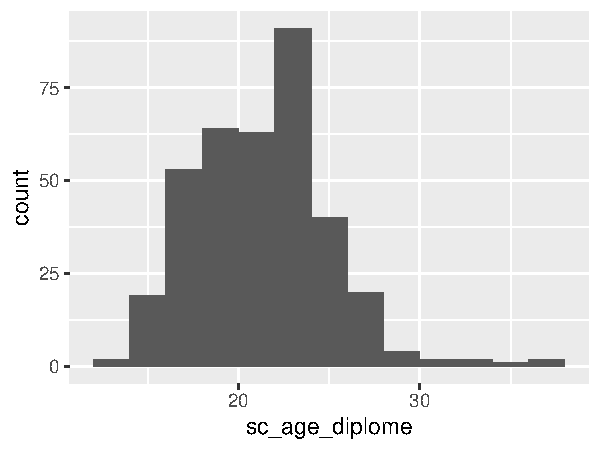
\includegraphics[keepaspectratio]{codebook_data_files/figure-pdf/Var-78-sc-age-diplome-1.pdf}}

\emini

\fullline

\subsection{sc\_rdb\_date\_creation}\label{sc_rdb_date_creation}

\bminione

\begin{longtable}[]{@{}lr@{}}
\toprule\noalign{}
Feature & Result \\
\midrule\noalign{}
\endhead
\bottomrule\noalign{}
\endlastfoot
Variable type & character \\
Number of missing obs. & 269 (59.25 \%) \\
Number of unique values & 121 \\
Mode & ``2017-05-09'' \\
\end{longtable}

\emini
\bminitwo

\pandocbounded{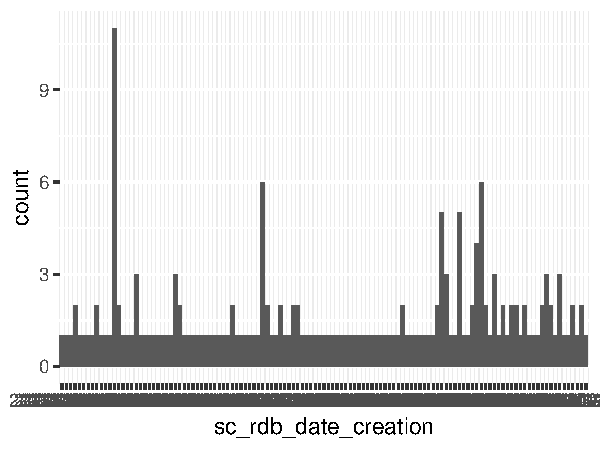
\includegraphics[keepaspectratio]{codebook_data_files/figure-pdf/Var-79-sc-rdb-date-creation-1.pdf}}

\emini

\begin{itemize}
\tightlist
\item
  Observed factor levels: ``2017-04-01'', ``2017-04-10'',
  ``2017-04-12'', ``2017-04-13'', ``2017-04-20'', ``2017-04-22'',
  ``2017-04-26'', ``2017-04-28'', ``2017-05-03'', ``2017-05-04'',
  ``2017-05-07'', ``2017-05-08'', ``2017-05-09'', ``2017-05-10'',
  ``2017-05-11'', ``2017-05-12'', ``2017-05-16'', ``2017-05-18'',
  ``2017-05-19'', ``2017-06-15'', ``2017-06-19'', ``2017-06-23'',
  ``2017-06-27'', ``2017-06-28'', ``2017-07-01'', ``2017-07-04'',
  ``2017-07-05'', ``2017-07-06'', ``2017-07-07'', ``2017-07-11'',
  ``2017-07-12'', ``2017-07-18'', ``2017-07-24'', ``2017-07-27'',
  ``2017-08-10'', ``2017-08-20'', ``2017-09-11'', ``2017-09-20'',
  ``2017-09-21'', ``2017-09-25'', ``2017-09-27'', ``2017-10-26'',
  ``2017-10-29'', ``2017-11-02'', ``2017-11-09'', ``2017-11-21'',
  ``2017-11-23'', ``2017-11-24'', ``2017-11-26'', ``2017-11-27'',
  ``2017-11-30'', ``2017-12-04'', ``2017-12-07'', ``2017-12-11'',
  ``2017-12-13'', ``2017-12-19'', ``2017-12-22'', ``2017-12-27'',
  ``2018-01-02'', ``2018-01-04'', ``2018-01-23'', ``2018-01-31'',
  ``2018-02-01'', ``2018-02-08'', ``2018-02-12'', ``2018-02-16'',
  ``2018-02-20'', ``2018-02-25'', ``2018-03-09'', ``2018-03-12'',
  ``2018-03-28'', ``2018-04-29'', ``2018-05-03'', ``2018-05-13'',
  ``2018-06-26'', ``2018-07-26'', ``2018-08-09'', ``2018-11-22'',
  ``2018-11-24'', ``2018-11-27'', ``2018-11-28'', ``2018-11-30'',
  ``2018-12-02'', ``2018-12-03'', ``2018-12-04'', ``2018-12-06'',
  ``2018-12-10'', ``2018-12-11'', ``2018-12-12'', ``2018-12-13'',
  ``2018-12-15'', ``2018-12-17'', ``2018-12-20'', ``2018-12-21'',
  ``2018-12-24'', ``2018-12-26'', ``2018-12-27'', ``2018-12-28'',
  ``2018-12-29'', ``2018-12-30'', ``2018-12-31'', ``2019-01-03'',
  ``2019-01-04'', ``2019-01-05'', ``2019-01-06'', ``2019-01-07'',
  ``2019-01-08'', ``2019-01-09'', ``2019-01-10'', ``2019-01-13'',
  ``2019-01-14'', ``2019-01-17'', ``2019-01-19'', ``2019-01-23'',
  ``2019-01-27'', ``2019-01-29'', ``2019-01-30'', ``2019-02-01'',
  ``2019-02-14'', ``2019-02-17'', ``2019-02-26''.
\end{itemize}

\fullline

\subsection{sc\_rdb\_nb}\label{sc_rdb_nb}

\bminione

\begin{longtable}[]{@{}lr@{}}
\toprule\noalign{}
Feature & Result \\
\midrule\noalign{}
\endhead
\bottomrule\noalign{}
\endlastfoot
Variable type & integer \\
Number of missing obs. & 269 (59.25 \%) \\
Number of unique values & 4 \\
Median & 1 \\
1st and 3rd quartiles & 1; 2 \\
Min. and max. & 1; 4 \\
\end{longtable}

\emini
\bminitwo

\pandocbounded{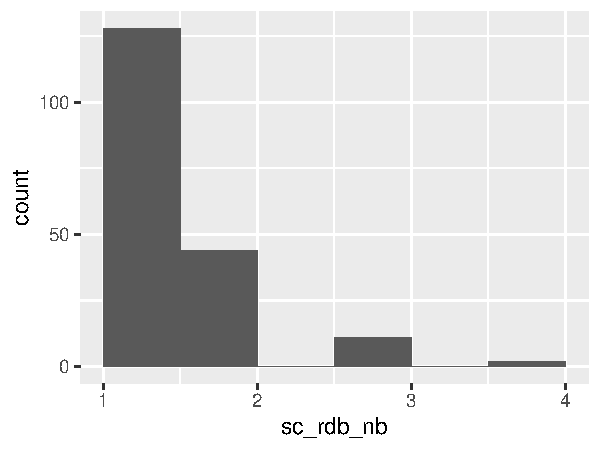
\includegraphics[keepaspectratio]{codebook_data_files/figure-pdf/Var-80-sc-rdb-nb-1.pdf}}

\emini

\fullline

\subsection{sc\_rdb\_type}\label{sc_rdb_type}

\begin{itemize}
\tightlist
\item
  The variable only takes one (non-missing) value: ``P''. The variable
  contains 59.25 \% missing observations.
\end{itemize}

\fullline

\subsection{sc\_rdb\_redoubl}\label{sc_rdb_redoubl}

\begin{itemize}
\tightlist
\item
  The variable only takes one (non-missing) value: ``1''. The variable
  contains 59.47 \% missing observations.
\end{itemize}

\fullline

\subsection{id\_age\_cat}\label{id_age_cat}

\bminione

\begin{longtable}[]{@{}lr@{}}
\toprule\noalign{}
Feature & Result \\
\midrule\noalign{}
\endhead
\bottomrule\noalign{}
\endlastfoot
Variable type & character \\
Number of missing obs. & 0 (0 \%) \\
Number of unique values & 2 \\
Mode & ``Adulte'' \\
\end{longtable}

\emini
\bminitwo

\pandocbounded{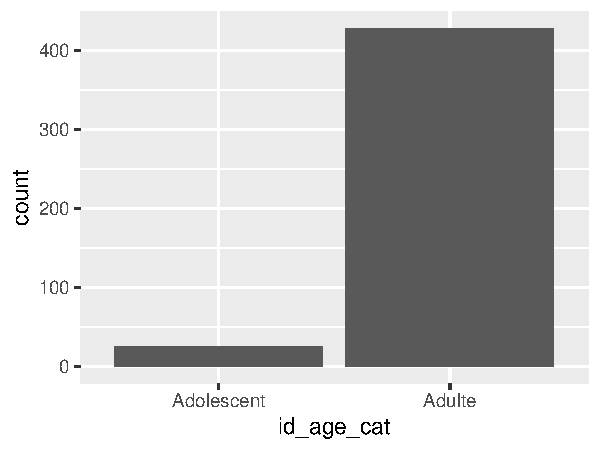
\includegraphics[keepaspectratio]{codebook_data_files/figure-pdf/Var-83-id-age-cat-1.pdf}}

\emini

\begin{itemize}
\tightlist
\item
  Observed factor levels: ``Adolescent'', ``Adulte''.
\end{itemize}

\fullline

\subsection{sc\_rdb\_cat}\label{sc_rdb_cat}

\begin{itemize}
\tightlist
\item
  The variable only takes one (non-missing) value: ``sc\_02\_rdb\_02''.
  The variable contains 59.25 \% missing observations.
\end{itemize}

\fullline

\subsection{sc\_rdb01\_an}\label{sc_rdb01_an}

\bminione

\begin{longtable}[]{@{}lr@{}}
\toprule\noalign{}
Feature & Result \\
\midrule\noalign{}
\endhead
\bottomrule\noalign{}
\endlastfoot
Variable type & integer \\
Number of missing obs. & 286 (63 \%) \\
Number of unique values & 45 \\
Median & 1998 \\
1st and 3rd quartiles & 1993; 2006 \\
Min. and max. & 1951; 2018 \\
\end{longtable}

\emini
\bminitwo

\pandocbounded{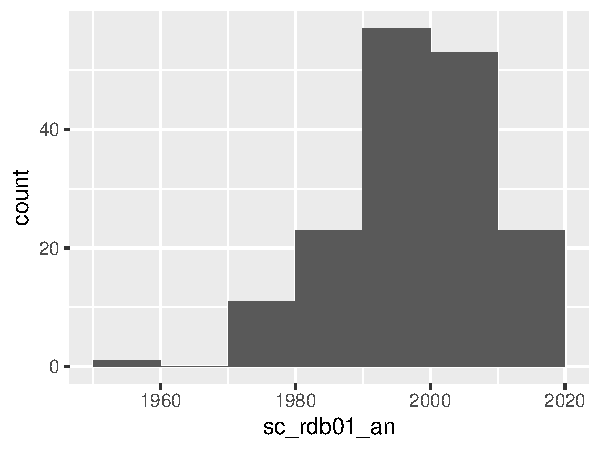
\includegraphics[keepaspectratio]{codebook_data_files/figure-pdf/Var-85-sc-rdb01-an-1.pdf}}

\emini

\fullline

\subsection{sc\_rdb02\_an}\label{sc_rdb02_an}

\bminione

\begin{longtable}[]{@{}lr@{}}
\toprule\noalign{}
Feature & Result \\
\midrule\noalign{}
\endhead
\bottomrule\noalign{}
\endlastfoot
Variable type & integer \\
Number of missing obs. & 402 (88.55 \%) \\
Number of unique values & 27 \\
Median & 1999 \\
1st and 3rd quartiles & 1993; 2008.25 \\
Min. and max. & 1978; 2017 \\
\end{longtable}

\emini
\bminitwo

\pandocbounded{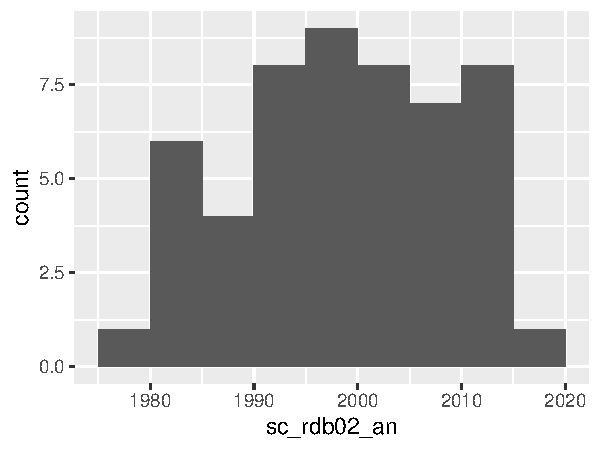
\includegraphics[keepaspectratio]{codebook_data_files/figure-pdf/Var-86-sc-rdb02-an-1.pdf}}

\emini

\fullline

\subsection{sc\_rdb03\_an}\label{sc_rdb03_an}

\bminione

\begin{longtable}[]{@{}lr@{}}
\toprule\noalign{}
Feature & Result \\
\midrule\noalign{}
\endhead
\bottomrule\noalign{}
\endlastfoot
Variable type & integer \\
Number of missing obs. & 442 (97.36 \%) \\
Number of unique values & 10 \\
Median & 2000 \\
1st and 3rd quartiles & 1991.75; 2005 \\
Min. and max. & 1987; 2012 \\
\end{longtable}

\emini
\bminitwo

\pandocbounded{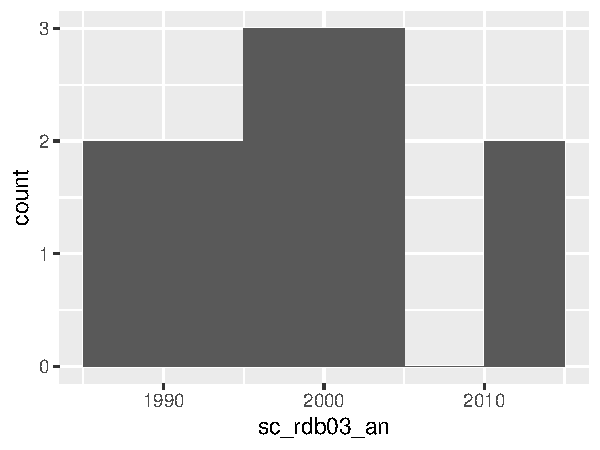
\includegraphics[keepaspectratio]{codebook_data_files/figure-pdf/Var-87-sc-rdb03-an-1.pdf}}

\emini

\fullline

\subsection{sc\_rdb04\_an}\label{sc_rdb04_an}

\bminione

\begin{longtable}[]{@{}lr@{}}
\toprule\noalign{}
Feature & Result \\
\midrule\noalign{}
\endhead
\bottomrule\noalign{}
\endlastfoot
Variable type & integer \\
Number of missing obs. & 452 (99.56 \%) \\
Number of unique values & 2 \\
Median & 1993.5 \\
1st and 3rd quartiles & 1993.25; 1993.75 \\
Min. and max. & 1993; 1994 \\
\end{longtable}

\emini
\bminitwo

\pandocbounded{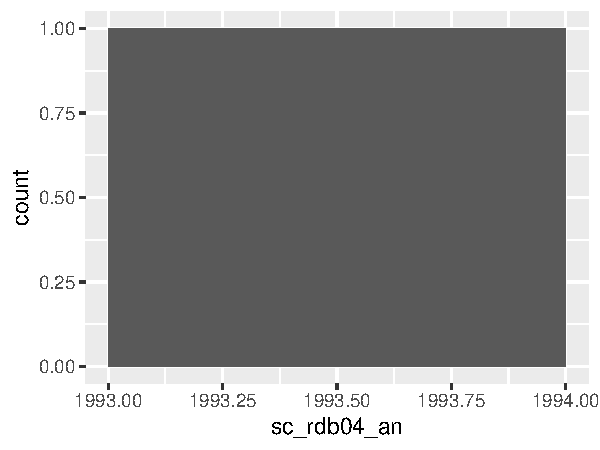
\includegraphics[keepaspectratio]{codebook_data_files/figure-pdf/Var-88-sc-rdb04-an-1.pdf}}

\emini

\fullline

\subsection{sc\_rdb01\_cause}\label{sc_rdb01_cause}

\bminione

\begin{longtable}[]{@{}lr@{}}
\toprule\noalign{}
Feature & Result \\
\midrule\noalign{}
\endhead
\bottomrule\noalign{}
\endlastfoot
Variable type & integer \\
Number of missing obs. & 272 (59.91 \%) \\
Number of unique values & 2 \\
Median & 0 \\
1st and 3rd quartiles & 0; 1 \\
Min. and max. & 0; 1 \\
\end{longtable}

\emini
\bminitwo

\pandocbounded{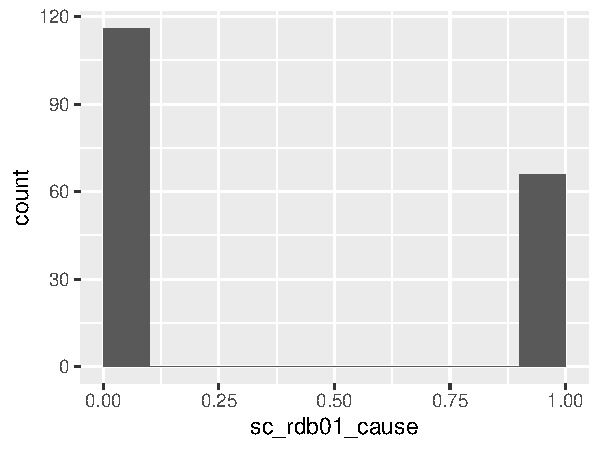
\includegraphics[keepaspectratio]{codebook_data_files/figure-pdf/Var-89-sc-rdb01-cause-1.pdf}}

\emini

\fullline

\subsection{sc\_rdb02\_cause}\label{sc_rdb02_cause}

\bminione

\begin{longtable}[]{@{}lr@{}}
\toprule\noalign{}
Feature & Result \\
\midrule\noalign{}
\endhead
\bottomrule\noalign{}
\endlastfoot
Variable type & integer \\
Number of missing obs. & 397 (87.44 \%) \\
Number of unique values & 2 \\
Median & 0 \\
1st and 3rd quartiles & 0; 1 \\
Min. and max. & 0; 1 \\
\end{longtable}

\emini
\bminitwo

\pandocbounded{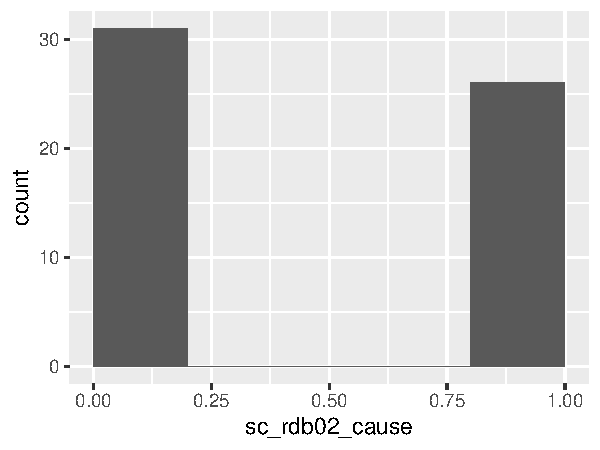
\includegraphics[keepaspectratio]{codebook_data_files/figure-pdf/Var-90-sc-rdb02-cause-1.pdf}}

\emini

\fullline

\subsection{sc\_rdb03\_cause}\label{sc_rdb03_cause}

\bminione

\begin{longtable}[]{@{}lr@{}}
\toprule\noalign{}
Feature & Result \\
\midrule\noalign{}
\endhead
\bottomrule\noalign{}
\endlastfoot
Variable type & integer \\
Number of missing obs. & 441 (97.14 \%) \\
Number of unique values & 2 \\
Median & 1 \\
1st and 3rd quartiles & 0; 1 \\
Min. and max. & 0; 1 \\
\end{longtable}

\emini
\bminitwo

\pandocbounded{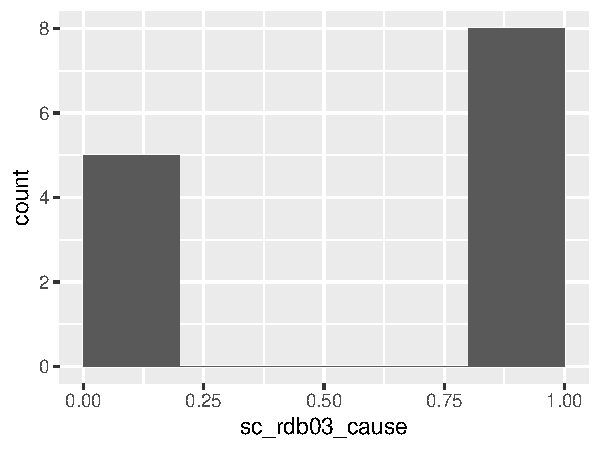
\includegraphics[keepaspectratio]{codebook_data_files/figure-pdf/Var-91-sc-rdb03-cause-1.pdf}}

\emini

\fullline

\subsection{sc\_rdb04\_cause}\label{sc_rdb04_cause}

\bminione

\begin{longtable}[]{@{}lr@{}}
\toprule\noalign{}
Feature & Result \\
\midrule\noalign{}
\endhead
\bottomrule\noalign{}
\endlastfoot
Variable type & integer \\
Number of missing obs. & 452 (99.56 \%) \\
Number of unique values & 2 \\
Median & 0.5 \\
1st and 3rd quartiles & 0.25; 0.75 \\
Min. and max. & 0; 1 \\
\end{longtable}

\emini
\bminitwo

\pandocbounded{\includegraphics[keepaspectratio]{codebook_data_files/figure-pdf/Var-92-sc-rdb04-cause-1.pdf}}

\emini

\fullline

\subsection{sc\_rdb01\_classe}\label{sc_rdb01_classe}

\bminione

\begin{longtable}[]{@{}lr@{}}
\toprule\noalign{}
Feature & Result \\
\midrule\noalign{}
\endhead
\bottomrule\noalign{}
\endlastfoot
Variable type & integer \\
Number of missing obs. & 270 (59.47 \%) \\
Number of unique values & 20 \\
Median & 10.5 \\
1st and 3rd quartiles & 6; 14 \\
Min. and max. & 1; 999 \\
\end{longtable}

\emini
\bminitwo

\pandocbounded{\includegraphics[keepaspectratio]{codebook_data_files/figure-pdf/Var-93-sc-rdb01-classe-1.pdf}}

\emini

\fullline

\subsection{sc\_rdb02\_classe}\label{sc_rdb02_classe}

\bminione

\begin{longtable}[]{@{}lr@{}}
\toprule\noalign{}
Feature & Result \\
\midrule\noalign{}
\endhead
\bottomrule\noalign{}
\endlastfoot
Variable type & integer \\
Number of missing obs. & 397 (87.44 \%) \\
Number of unique values & 19 \\
Median & 14 \\
1st and 3rd quartiles & 9; 19 \\
Min. and max. & 2; 999 \\
\end{longtable}

\emini
\bminitwo

\pandocbounded{\includegraphics[keepaspectratio]{codebook_data_files/figure-pdf/Var-94-sc-rdb02-classe-1.pdf}}

\emini

\fullline

\subsection{sc\_rdb03\_classe}\label{sc_rdb03_classe}

\bminione

\begin{longtable}[]{@{}lr@{}}
\toprule\noalign{}
Feature & Result \\
\midrule\noalign{}
\endhead
\bottomrule\noalign{}
\endlastfoot
Variable type & integer \\
Number of missing obs. & 441 (97.14 \%) \\
Number of unique values & 9 \\
Median & 20 \\
1st and 3rd quartiles & 14; 21 \\
Min. and max. & 9; 999 \\
\end{longtable}

\emini
\bminitwo

\pandocbounded{\includegraphics[keepaspectratio]{codebook_data_files/figure-pdf/Var-95-sc-rdb03-classe-1.pdf}}

\emini

\fullline

\subsection{sc\_rdb04\_classe}\label{sc_rdb04_classe}

\bminione

\begin{longtable}[]{@{}lr@{}}
\toprule\noalign{}
Feature & Result \\
\midrule\noalign{}
\endhead
\bottomrule\noalign{}
\endlastfoot
Variable type & integer \\
Number of missing obs. & 452 (99.56 \%) \\
Number of unique values & 2 \\
Median & 21 \\
1st and 3rd quartiles & 20.5; 21.5 \\
Min. and max. & 20; 22 \\
\end{longtable}

\emini
\bminitwo

\pandocbounded{\includegraphics[keepaspectratio]{codebook_data_files/figure-pdf/Var-96-sc-rdb04-classe-1.pdf}}

\emini

\fullline

\subsection{sc\_rdb01\_classe\_autre}\label{sc_rdb01_classe_autre}

\bminione

\begin{longtable}[]{@{}lr@{}}
\toprule\noalign{}
Feature & Result \\
\midrule\noalign{}
\endhead
\bottomrule\noalign{}
\endlastfoot
Variable type & character \\
Number of missing obs. & 451 (99.34 \%) \\
Number of unique values & 3 \\
Mode & ``2e année d'architecture d'intèrieur'' \\
\end{longtable}

\emini
\bminitwo

\pandocbounded{\includegraphics[keepaspectratio]{codebook_data_files/figure-pdf/Var-97-sc-rdb01-classe-autre-1.pdf}}

\emini

\begin{itemize}
\tightlist
\item
  Observed factor levels: ``2e année d'architecture d'intèrieur'', ``BEP
  en 3 ans'', ``Paces''.
\end{itemize}

\fullline

\subsection{sc\_rdb02\_classe\_autre}\label{sc_rdb02_classe_autre}

\begin{itemize}
\tightlist
\item
  The variable only takes one (non-missing) value: ``3e année d'étude
  d'auxiliaire puéricultrice(belges''. The variable contains 99.78 \%
  missing observations.
\end{itemize}

\fullline

\subsection{sc\_rdb03\_classe\_autre}\label{sc_rdb03_classe_autre}

\begin{itemize}
\tightlist
\item
  The variable only takes one (non-missing) value: ``5eme année de
  médecine''. The variable contains 99.78 \% missing observations.
\end{itemize}

\fullline

\subsection{sc\_rdb01\_classe\_cat}\label{sc_rdb01_classe_cat}

\bminione

\begin{longtable}[]{@{}lr@{}}
\toprule\noalign{}
Feature & Result \\
\midrule\noalign{}
\endhead
\bottomrule\noalign{}
\endlastfoot
Variable type & character \\
Number of missing obs. & 270 (59.47 \%) \\
Number of unique values & 4 \\
Mode & ``3-Lycée'' \\
\end{longtable}

\emini
\bminitwo

\pandocbounded{\includegraphics[keepaspectratio]{codebook_data_files/figure-pdf/Var-100-sc-rdb01-classe-cat-1.pdf}}

\emini

\begin{itemize}
\tightlist
\item
  Observed factor levels: ``1-Ecole élémentaire'', ``2-Collège'',
  ``3-Lycée'', ``4-Supérieur''.
\end{itemize}

\fullline

\subsection{sc\_rdb02\_classe\_cat}\label{sc_rdb02_classe_cat}

\bminione

\begin{longtable}[]{@{}lr@{}}
\toprule\noalign{}
Feature & Result \\
\midrule\noalign{}
\endhead
\bottomrule\noalign{}
\endlastfoot
Variable type & character \\
Number of missing obs. & 397 (87.44 \%) \\
Number of unique values & 4 \\
Mode & ``3-Lycée'' \\
\end{longtable}

\emini
\bminitwo

\pandocbounded{\includegraphics[keepaspectratio]{codebook_data_files/figure-pdf/Var-101-sc-rdb02-classe-cat-1.pdf}}

\emini

\begin{itemize}
\tightlist
\item
  Observed factor levels: ``1-Ecole élémentaire'', ``2-Collège'',
  ``3-Lycée'', ``4-Supérieur''.
\end{itemize}

\fullline

\subsection{sc\_rdb03\_classe\_cat}\label{sc_rdb03_classe_cat}

\bminione

\begin{longtable}[]{@{}lr@{}}
\toprule\noalign{}
Feature & Result \\
\midrule\noalign{}
\endhead
\bottomrule\noalign{}
\endlastfoot
Variable type & character \\
Number of missing obs. & 441 (97.14 \%) \\
Number of unique values & 3 \\
Mode & ``4-Supérieur'' \\
\end{longtable}

\emini
\bminitwo

\pandocbounded{\includegraphics[keepaspectratio]{codebook_data_files/figure-pdf/Var-102-sc-rdb03-classe-cat-1.pdf}}

\emini

\begin{itemize}
\tightlist
\item
  Observed factor levels: ``2-Collège'', ``3-Lycée'', ``4-Supérieur''.
\end{itemize}

\fullline

\subsection{sc\_rdb04\_classe\_cat}\label{sc_rdb04_classe_cat}

\begin{itemize}
\tightlist
\item
  The variable only takes one (non-missing) value: ``4-Supérieur''. The
  variable contains 99.56 \% missing observations.
\end{itemize}

\fullline

\subsection{sc\_int\_date\_creation}\label{sc_int_date_creation}

\bminione

\begin{longtable}[]{@{}lr@{}}
\toprule\noalign{}
Feature & Result \\
\midrule\noalign{}
\endhead
\bottomrule\noalign{}
\endlastfoot
Variable type & character \\
Number of missing obs. & 372 (81.94 \%) \\
Number of unique values & 61 \\
Mode & ``2017-05-09'' \\
\end{longtable}

\emini
\bminitwo

\pandocbounded{\includegraphics[keepaspectratio]{codebook_data_files/figure-pdf/Var-104-sc-int-date-creation-1.pdf}}

\emini

\begin{itemize}
\tightlist
\item
  Observed factor levels: ``2017-04-01'', ``2017-04-10'',
  ``2017-04-11'', ``2017-04-20'', ``2017-04-25'', ``2017-04-26'',
  ``2017-04-27'', ``2017-05-02'', ``2017-05-03'', ``2017-05-09'',
  ``2017-05-10'', ``2017-05-11'', ``2017-05-12'', ``2017-05-16'',
  ``2017-05-19'', ``2017-05-28'', ``2017-06-29'', ``2017-07-05'',
  ``2017-07-11'', ``2017-07-24'', ``2017-07-27'', ``2017-10-05'',
  ``2017-11-23'', ``2017-11-24'', ``2017-11-26'', ``2017-12-04'',
  ``2017-12-11'', ``2017-12-12'', ``2017-12-19'', ``2018-01-02'',
  ``2018-01-04'', ``2018-01-23'', ``2018-01-27'', ``2018-02-12'',
  ``2018-02-16'', ``2018-02-20'', ``2018-03-12'', ``2018-03-28'',
  ``2018-05-03'', ``2018-06-26'', ``2018-11-22'', ``2018-11-30'',
  ``2018-12-02'', ``2018-12-03'', ``2018-12-04'', ``2018-12-10'',
  ``2018-12-11'', ``2018-12-24'', ``2018-12-26'', ``2018-12-27'',
  ``2018-12-28'', ``2018-12-29'', ``2019-01-01'', ``2019-01-06'',
  ``2019-01-08'', ``2019-01-09'', ``2019-01-14'', ``2019-01-17'',
  ``2019-01-18'', ``2019-01-23'', ``2019-02-14''.
\end{itemize}

\fullline

\subsection{sc\_int\_nb}\label{sc_int_nb}

\bminione

\begin{longtable}[]{@{}lr@{}}
\toprule\noalign{}
Feature & Result \\
\midrule\noalign{}
\endhead
\bottomrule\noalign{}
\endlastfoot
Variable type & integer \\
Number of missing obs. & 372 (81.94 \%) \\
Number of unique values & 6 \\
Median & 1 \\
1st and 3rd quartiles & 1; 2 \\
Min. and max. & 1; 8 \\
\end{longtable}

\emini
\bminitwo

\pandocbounded{\includegraphics[keepaspectratio]{codebook_data_files/figure-pdf/Var-105-sc-int-nb-1.pdf}}

\emini

\fullline

\subsection{sc\_int\_type}\label{sc_int_type}

\begin{itemize}
\tightlist
\item
  The variable only takes one (non-missing) value: ``P''. The variable
  contains 81.94 \% missing observations.
\end{itemize}

\fullline

\subsection{sc\_int\_interromp}\label{sc_int_interromp}

\begin{itemize}
\tightlist
\item
  The variable only takes one (non-missing) value: ``1''. The variable
  contains 81.94 \% missing observations.
\end{itemize}

\fullline

\subsection{sc\_int\_cat}\label{sc_int_cat}

\begin{itemize}
\tightlist
\item
  The variable only takes one (non-missing) value: ``sc\_02\_int\_02''.
  The variable contains 81.94 \% missing observations.
\end{itemize}

\fullline

\subsection{sc\_int01\_classe}\label{sc_int01_classe}

\bminione

\begin{longtable}[]{@{}lr@{}}
\toprule\noalign{}
Feature & Result \\
\midrule\noalign{}
\endhead
\bottomrule\noalign{}
\endlastfoot
Variable type & integer \\
Number of missing obs. & 380 (83.7 \%) \\
Number of unique values & 20 \\
Median & 12.5 \\
1st and 3rd quartiles & 7; 19 \\
Min. and max. & 1; 999 \\
\end{longtable}

\emini
\bminitwo

\pandocbounded{\includegraphics[keepaspectratio]{codebook_data_files/figure-pdf/Var-109-sc-int01-classe-1.pdf}}

\emini

\fullline

\subsection{sc\_int02\_classe}\label{sc_int02_classe}

\bminione

\begin{longtable}[]{@{}lr@{}}
\toprule\noalign{}
Feature & Result \\
\midrule\noalign{}
\endhead
\bottomrule\noalign{}
\endlastfoot
Variable type & integer \\
Number of missing obs. & 432 (95.15 \%) \\
Number of unique values & 14 \\
Median & 13 \\
1st and 3rd quartiles & 9.75; 21 \\
Min. and max. & 2; 999 \\
\end{longtable}

\emini
\bminitwo

\pandocbounded{\includegraphics[keepaspectratio]{codebook_data_files/figure-pdf/Var-110-sc-int02-classe-1.pdf}}

\emini

\fullline

\subsection{sc\_int03\_classe}\label{sc_int03_classe}

\bminione

\begin{longtable}[]{@{}lr@{}}
\toprule\noalign{}
Feature & Result \\
\midrule\noalign{}
\endhead
\bottomrule\noalign{}
\endlastfoot
Variable type & integer \\
Number of missing obs. & 444 (97.8 \%) \\
Number of unique values & 7 \\
Median & 13 \\
1st and 3rd quartiles & 12.25; 19.5 \\
Min. and max. & 7; 26 \\
\end{longtable}

\emini
\bminitwo

\pandocbounded{\includegraphics[keepaspectratio]{codebook_data_files/figure-pdf/Var-111-sc-int03-classe-1.pdf}}

\emini

\fullline

\subsection{sc\_int04\_classe}\label{sc_int04_classe}

\bminione

\begin{longtable}[]{@{}lr@{}}
\toprule\noalign{}
Feature & Result \\
\midrule\noalign{}
\endhead
\bottomrule\noalign{}
\endlastfoot
Variable type & integer \\
Number of missing obs. & 449 (98.9 \%) \\
Number of unique values & 4 \\
Median & 19 \\
1st and 3rd quartiles & 13; 21 \\
Min. and max. & 8; 21 \\
\end{longtable}

\emini
\bminitwo

\pandocbounded{\includegraphics[keepaspectratio]{codebook_data_files/figure-pdf/Var-112-sc-int04-classe-1.pdf}}

\emini

\fullline

\subsection{sc\_int05\_classe}\label{sc_int05_classe}

\bminione

\begin{longtable}[]{@{}lr@{}}
\toprule\noalign{}
Feature & Result \\
\midrule\noalign{}
\endhead
\bottomrule\noalign{}
\endlastfoot
Variable type & integer \\
Number of missing obs. & 452 (99.56 \%) \\
Number of unique values & 2 \\
Median & 11.5 \\
1st and 3rd quartiles & 10.25; 12.75 \\
Min. and max. & 9; 14 \\
\end{longtable}

\emini
\bminitwo

\pandocbounded{\includegraphics[keepaspectratio]{codebook_data_files/figure-pdf/Var-113-sc-int05-classe-1.pdf}}

\emini

\fullline

\subsection{sc\_int06\_classe}\label{sc_int06_classe}

\begin{itemize}
\tightlist
\item
  The variable only takes one (non-missing) value: ``12''. The variable
  contains 99.78 \% missing observations.
\end{itemize}

\fullline

\subsection{sc\_int07\_classe}\label{sc_int07_classe}

\begin{itemize}
\tightlist
\item
  The variable only takes one (non-missing) value: ``13''. The variable
  contains 99.78 \% missing observations.
\end{itemize}

\fullline

\subsection{sc\_int08\_classe}\label{sc_int08_classe}

\begin{itemize}
\tightlist
\item
  The variable only takes one (non-missing) value: ``14''. The variable
  contains 99.78 \% missing observations.
\end{itemize}

\fullline

\subsection{sc\_int01\_an}\label{sc_int01_an}

\bminione

\begin{longtable}[]{@{}lr@{}}
\toprule\noalign{}
Feature & Result \\
\midrule\noalign{}
\endhead
\bottomrule\noalign{}
\endlastfoot
Variable type & integer \\
Number of missing obs. & 377 (83.04 \%) \\
Number of unique values & 30 \\
Median & 2006 \\
1st and 3rd quartiles & 1996; 2010 \\
Min. and max. & 1951; 2017 \\
\end{longtable}

\emini
\bminitwo

\pandocbounded{\includegraphics[keepaspectratio]{codebook_data_files/figure-pdf/Var-117-sc-int01-an-1.pdf}}

\emini

\fullline

\subsection{sc\_int02\_an}\label{sc_int02_an}

\bminione

\begin{longtable}[]{@{}lr@{}}
\toprule\noalign{}
Feature & Result \\
\midrule\noalign{}
\endhead
\bottomrule\noalign{}
\endlastfoot
Variable type & integer \\
Number of missing obs. & 433 (95.37 \%) \\
Number of unique values & 15 \\
Median & 2009 \\
1st and 3rd quartiles & 2001; 2013 \\
Min. and max. & 1983; 2017 \\
\end{longtable}

\emini
\bminitwo

\pandocbounded{\includegraphics[keepaspectratio]{codebook_data_files/figure-pdf/Var-118-sc-int02-an-1.pdf}}

\emini

\fullline

\subsection{sc\_int03\_an}\label{sc_int03_an}

\bminione

\begin{longtable}[]{@{}lr@{}}
\toprule\noalign{}
Feature & Result \\
\midrule\noalign{}
\endhead
\bottomrule\noalign{}
\endlastfoot
Variable type & integer \\
Number of missing obs. & 446 (98.24 \%) \\
Number of unique values & 7 \\
Median & 2014.5 \\
1st and 3rd quartiles & 2002.5; 2015.25 \\
Min. and max. & 1987; 2017 \\
\end{longtable}

\emini
\bminitwo

\pandocbounded{\includegraphics[keepaspectratio]{codebook_data_files/figure-pdf/Var-119-sc-int03-an-1.pdf}}

\emini

\fullline

\subsection{sc\_int04\_an}\label{sc_int04_an}

\bminione

\begin{longtable}[]{@{}lr@{}}
\toprule\noalign{}
Feature & Result \\
\midrule\noalign{}
\endhead
\bottomrule\noalign{}
\endlastfoot
Variable type & integer \\
Number of missing obs. & 450 (99.12 \%) \\
Number of unique values & 4 \\
Median & 2007.5 \\
1st and 3rd quartiles & 2003.75; 2012.25 \\
Min. and max. & 2003; 2016 \\
\end{longtable}

\emini
\bminitwo

\pandocbounded{\includegraphics[keepaspectratio]{codebook_data_files/figure-pdf/Var-120-sc-int04-an-1.pdf}}

\emini

\fullline

\subsection{sc\_int05\_an}\label{sc_int05_an}

\begin{itemize}
\tightlist
\item
  The variable only takes one (non-missing) value: ``2005''. The
  variable contains 99.78 \% missing observations.
\end{itemize}

\fullline

\subsection{sc\_int01\_an\_repr}\label{sc_int01_an_repr}

\bminione

\begin{longtable}[]{@{}lr@{}}
\toprule\noalign{}
Feature & Result \\
\midrule\noalign{}
\endhead
\bottomrule\noalign{}
\endlastfoot
Variable type & integer \\
Number of missing obs. & 384 (84.58 \%) \\
Number of unique values & 30 \\
Median & 2005 \\
1st and 3rd quartiles & 1996.25; 2011 \\
Min. and max. & 1952; 2017 \\
\end{longtable}

\emini
\bminitwo

\pandocbounded{\includegraphics[keepaspectratio]{codebook_data_files/figure-pdf/Var-122-sc-int01-an-repr-1.pdf}}

\emini

\fullline

\subsection{sc\_int02\_an\_repr}\label{sc_int02_an_repr}

\bminione

\begin{longtable}[]{@{}lr@{}}
\toprule\noalign{}
Feature & Result \\
\midrule\noalign{}
\endhead
\bottomrule\noalign{}
\endlastfoot
Variable type & integer \\
Number of missing obs. & 434 (95.59 \%) \\
Number of unique values & 16 \\
Median & 2011 \\
1st and 3rd quartiles & 2001.5; 2015 \\
Min. and max. & 1983; 2017 \\
\end{longtable}

\emini
\bminitwo

\pandocbounded{\includegraphics[keepaspectratio]{codebook_data_files/figure-pdf/Var-123-sc-int02-an-repr-1.pdf}}

\emini

\fullline

\subsection{sc\_int03\_an\_repr}\label{sc_int03_an_repr}

\bminione

\begin{longtable}[]{@{}lr@{}}
\toprule\noalign{}
Feature & Result \\
\midrule\noalign{}
\endhead
\bottomrule\noalign{}
\endlastfoot
Variable type & integer \\
Number of missing obs. & 447 (98.46 \%) \\
Number of unique values & 6 \\
Median & 2014 \\
1st and 3rd quartiles & 2002.5; 2017 \\
Min. and max. & 1989; 2018 \\
\end{longtable}

\emini
\bminitwo

\pandocbounded{\includegraphics[keepaspectratio]{codebook_data_files/figure-pdf/Var-124-sc-int03-an-repr-1.pdf}}

\emini

\fullline

\subsection{sc\_int04\_an\_repr}\label{sc_int04_an_repr}

\bminione

\begin{longtable}[]{@{}lr@{}}
\toprule\noalign{}
Feature & Result \\
\midrule\noalign{}
\endhead
\bottomrule\noalign{}
\endlastfoot
Variable type & integer \\
Number of missing obs. & 452 (99.56 \%) \\
Number of unique values & 2 \\
Median & 2004 \\
1st and 3rd quartiles & 2003.5; 2004.5 \\
Min. and max. & 2003; 2005 \\
\end{longtable}

\emini
\bminitwo

\pandocbounded{\includegraphics[keepaspectratio]{codebook_data_files/figure-pdf/Var-125-sc-int04-an-repr-1.pdf}}

\emini

\fullline

\subsection{sc\_int05\_an\_repr}\label{sc_int05_an_repr}

\begin{itemize}
\tightlist
\item
  The variable only takes one (non-missing) value: ``2006''. The
  variable contains 99.78 \% missing observations.
\end{itemize}

\fullline

\subsection{sc\_int01\_cause\_1}\label{sc_int01_cause_1}

\begin{itemize}
\tightlist
\item
  The variable only takes one (non-missing) value: ``1''. The variable
  contains 94.93 \% missing observations.
\end{itemize}

\fullline

\subsection{sc\_int02\_cause\_1}\label{sc_int02_cause_1}

\begin{itemize}
\tightlist
\item
  The variable only takes one (non-missing) value: ``1''. The variable
  contains 98.46 \% missing observations.
\end{itemize}

\fullline

\subsection{sc\_int03\_cause\_1}\label{sc_int03_cause_1}

\begin{itemize}
\tightlist
\item
  The variable only takes one (non-missing) value: ``1''. The variable
  contains 99.56 \% missing observations.
\end{itemize}

\fullline

\subsection{sc\_int04\_cause\_1}\label{sc_int04_cause_1}

\begin{itemize}
\tightlist
\item
  The variable only takes one (non-missing) value: ``1''. The variable
  contains 99.78 \% missing observations.
\end{itemize}

\fullline

\subsection{sc\_int01\_cause\_2}\label{sc_int01_cause_2}

\begin{itemize}
\tightlist
\item
  The variable only takes one (non-missing) value: ``1''. The variable
  contains 89.21 \% missing observations.
\end{itemize}

\fullline

\subsection{sc\_int02\_cause\_2}\label{sc_int02_cause_2}

\begin{itemize}
\tightlist
\item
  The variable only takes one (non-missing) value: ``1''. The variable
  contains 96.92 \% missing observations.
\end{itemize}

\fullline

\subsection{sc\_int03\_cause\_2}\label{sc_int03_cause_2}

\begin{itemize}
\tightlist
\item
  The variable only takes one (non-missing) value: ``1''. The variable
  contains 99.34 \% missing observations.
\end{itemize}

\fullline

\subsection{sc\_int01\_cause\_3}\label{sc_int01_cause_3}

\begin{itemize}
\tightlist
\item
  The variable only takes one (non-missing) value: ``1''. The variable
  contains 94.05 \% missing observations.
\end{itemize}

\fullline

\subsection{sc\_int02\_cause\_3}\label{sc_int02_cause_3}

\begin{itemize}
\tightlist
\item
  The variable only takes one (non-missing) value: ``1''. The variable
  contains 98.46 \% missing observations.
\end{itemize}

\fullline

\subsection{sc\_int03\_cause\_3}\label{sc_int03_cause_3}

\begin{itemize}
\tightlist
\item
  The variable only takes one (non-missing) value: ``1''. The variable
  contains 99.56 \% missing observations.
\end{itemize}

\fullline

\subsection{sc\_int04\_cause\_3}\label{sc_int04_cause_3}

\begin{itemize}
\tightlist
\item
  The variable only takes one (non-missing) value: ``1''. The variable
  contains 99.56 \% missing observations.
\end{itemize}

\fullline

\subsection{sc\_int05\_cause\_3}\label{sc_int05_cause_3}

\begin{itemize}
\tightlist
\item
  The variable only takes one (non-missing) value: ``1''. The variable
  contains 99.78 \% missing observations.
\end{itemize}

\fullline

\subsection{sc\_int01\_cause\_4}\label{sc_int01_cause_4}

\begin{itemize}
\tightlist
\item
  The variable only takes one (non-missing) value: ``1''. The variable
  contains 99.12 \% missing observations.
\end{itemize}

\fullline

\subsection{sc\_int04\_cause\_4}\label{sc_int04_cause_4}

\begin{itemize}
\tightlist
\item
  The variable only takes one (non-missing) value: ``1''. The variable
  contains 99.78 \% missing observations.
\end{itemize}

\fullline

\subsection{sc\_int01\_cause\_999}\label{sc_int01_cause_999}

\begin{itemize}
\tightlist
\item
  The variable only takes one (non-missing) value: ``1''. The variable
  contains 95.15 \% missing observations.
\end{itemize}

\fullline

\subsection{sc\_int02\_cause\_999}\label{sc_int02_cause_999}

\begin{itemize}
\tightlist
\item
  The variable only takes one (non-missing) value: ``1''. The variable
  contains 98.68 \% missing observations.
\end{itemize}

\fullline

\subsection{sc\_int03\_cause\_999}\label{sc_int03_cause_999}

\begin{itemize}
\tightlist
\item
  The variable only takes one (non-missing) value: ``1''. The variable
  contains 99.34 \% missing observations.
\end{itemize}

\fullline

\subsection{sc\_int01\_cause\_autre}\label{sc_int01_cause_autre}

\bminione

\begin{longtable}[]{@{}
  >{\raggedright\arraybackslash}p{(\linewidth - 2\tabcolsep) * \real{0.3472}}
  >{\raggedleft\arraybackslash}p{(\linewidth - 2\tabcolsep) * \real{0.6528}}@{}}
\toprule\noalign{}
\begin{minipage}[b]{\linewidth}\raggedright
Feature
\end{minipage} & \begin{minipage}[b]{\linewidth}\raggedleft
Result
\end{minipage} \\
\midrule\noalign{}
\endhead
\bottomrule\noalign{}
\endlastfoot
Variable type & character \\
Number of missing obs. & 433 (95.37 \%) \\
Number of unique values & 21 \\
Mode & ``6 mois en maison de santé de La Croix Rouge'' \\
\end{longtable}

\emini
\bminitwo

\pandocbounded{\includegraphics[keepaspectratio]{codebook_data_files/figure-pdf/Var-144-sc-int01-cause-autre-1.pdf}}

\emini

\begin{itemize}
\tightlist
\item
  Observed factor levels: ``6 mois en maison de santé de La Croix
  Rouge'', ``Antibiotiques en perfusion prévu initialement pour 3
  mois'', ``Attente de greffe'', ``Besoin de repos a cause d?anxiete'',
  ``cure thermale'', ``CURES PERFUSIONS ANTIBIOTIQUES'', ``Décès de mon
  frère entraînant une aggravation de mon état de santé, conduisant à la
  greffe'', ``Décompensation'', ``DEPRESSION PHOBIE SOCIALE /SCOLAIRE'',
  ``diagnostic tardif de la muco et début du diabète'', ``douleurs non
  reconnue dû à la muco'', ``état dépressif et perfusion très fréquente
  (1/ mois)'', ``fatigue'', ``Grippe'', ``Hospitalisation a domicile
  cure antibiotiques par intraveineuse'', ``Oxygénothérapie, dégradation
  de l'état général..'', ``perfusion'', ``prevention Grippe H1N1'',
  ``Stage à l'étranger obligatoire non compatible avec ma santé'',
  ``traitements lourds par intraveineuses contre pyocianique'', ``Trop
  fatiguée pour poursuivre''.
\end{itemize}

\fullline

\subsection{sc\_int02\_cause\_autre}\label{sc_int02_cause_autre}

\bminione

\begin{longtable}[]{@{}lr@{}}
\toprule\noalign{}
Feature & Result \\
\midrule\noalign{}
\endhead
\bottomrule\noalign{}
\endlastfoot
Variable type & character \\
Number of missing obs. & 448 (98.68 \%) \\
Number of unique values & 6 \\
Mode & ``Dépression'' \\
\end{longtable}

\emini
\bminitwo

\pandocbounded{\includegraphics[keepaspectratio]{codebook_data_files/figure-pdf/Var-145-sc-int02-cause-autre-1.pdf}}

\emini

\begin{itemize}
\tightlist
\item
  Observed factor levels: ``Dépression'', ``Hospitalisation cure
  antibiotiques par voie intraveineuse'', ``Hospitalisation
  Psychatrique'', ``hypertension, grippe etc\ldots{}'', ``infection
  traitement par perfusion à la maison'', ``projet greffe''.
\end{itemize}

\fullline

\subsection{sc\_int03\_cause\_autre}\label{sc_int03_cause_autre}

\bminione

\begin{longtable}[]{@{}lr@{}}
\toprule\noalign{}
Feature & Result \\
\midrule\noalign{}
\endhead
\bottomrule\noalign{}
\endlastfoot
Variable type & character \\
Number of missing obs. & 451 (99.34 \%) \\
Number of unique values & 3 \\
Mode & ``anemie, douleurs thoraciques, dépression'' \\
\end{longtable}

\emini
\bminitwo

\pandocbounded{\includegraphics[keepaspectratio]{codebook_data_files/figure-pdf/Var-146-sc-int03-cause-autre-1.pdf}}

\emini

\begin{itemize}
\tightlist
\item
  Observed factor levels: ``anemie, douleurs thoraciques, dépression'',
  ``Cas de grippe HAN1'', ``fatigue''.
\end{itemize}

\fullline

\subsection{sc\_int01\_classe\_autre}\label{sc_int01_classe_autre}

\bminione

\begin{longtable}[]{@{}lr@{}}
\toprule\noalign{}
Feature & Result \\
\midrule\noalign{}
\endhead
\bottomrule\noalign{}
\endlastfoot
Variable type & character \\
Number of missing obs. & 450 (99.12 \%) \\
Number of unique values & 4 \\
Mode & ``2e année d'architecture d'intèrieur'' \\
\end{longtable}

\emini
\bminitwo

\pandocbounded{\includegraphics[keepaspectratio]{codebook_data_files/figure-pdf/Var-147-sc-int01-classe-autre-1.pdf}}

\emini

\begin{itemize}
\tightlist
\item
  Observed factor levels: ``2e année d'architecture d'intèrieur'',
  ``3eme année préparation CAP cuisine hôtelerie'', ``5eme année de
  médecine'', ``BEP''.
\end{itemize}

\fullline

\subsection{sc\_int02\_classe\_autre}\label{sc_int02_classe_autre}

\begin{itemize}
\tightlist
\item
  The variable only takes one (non-missing) value: ``BEP Agent
  Administratif des Entreprises''. The variable contains 99.78 \%
  missing observations.
\end{itemize}

\fullline

\subsection{sc\_int01\_classe\_repr}\label{sc_int01_classe_repr}

\bminione

\begin{longtable}[]{@{}lr@{}}
\toprule\noalign{}
Feature & Result \\
\midrule\noalign{}
\endhead
\bottomrule\noalign{}
\endlastfoot
Variable type & integer \\
Number of missing obs. & 376 (82.82 \%) \\
Number of unique values & 19 \\
Median & 13 \\
1st and 3rd quartiles & 7; 20 \\
Min. and max. & 1; 999 \\
\end{longtable}

\emini
\bminitwo

\pandocbounded{\includegraphics[keepaspectratio]{codebook_data_files/figure-pdf/Var-149-sc-int01-classe-repr-1.pdf}}

\emini

\fullline

\subsection{sc\_int02\_classe\_repr}\label{sc_int02_classe_repr}

\bminione

\begin{longtable}[]{@{}lr@{}}
\toprule\noalign{}
Feature & Result \\
\midrule\noalign{}
\endhead
\bottomrule\noalign{}
\endlastfoot
Variable type & integer \\
Number of missing obs. & 432 (95.15 \%) \\
Number of unique values & 13 \\
Median & 13 \\
1st and 3rd quartiles & 12; 19.75 \\
Min. and max. & 2; 999 \\
\end{longtable}

\emini
\bminitwo

\pandocbounded{\includegraphics[keepaspectratio]{codebook_data_files/figure-pdf/Var-150-sc-int02-classe-repr-1.pdf}}

\emini

\fullline

\subsection{sc\_int03\_classe\_repr}\label{sc_int03_classe_repr}

\bminione

\begin{longtable}[]{@{}lr@{}}
\toprule\noalign{}
Feature & Result \\
\midrule\noalign{}
\endhead
\bottomrule\noalign{}
\endlastfoot
Variable type & integer \\
Number of missing obs. & 446 (98.24 \%) \\
Number of unique values & 7 \\
Median & 13.5 \\
1st and 3rd quartiles & 12; 22 \\
Min. and max. & 7; 26 \\
\end{longtable}

\emini
\bminitwo

\pandocbounded{\includegraphics[keepaspectratio]{codebook_data_files/figure-pdf/Var-151-sc-int03-classe-repr-1.pdf}}

\emini

\fullline

\subsection{sc\_int04\_classe\_repr}\label{sc_int04_classe_repr}

\bminione

\begin{longtable}[]{@{}lr@{}}
\toprule\noalign{}
Feature & Result \\
\midrule\noalign{}
\endhead
\bottomrule\noalign{}
\endlastfoot
Variable type & integer \\
Number of missing obs. & 452 (99.56 \%) \\
Number of unique values & 2 \\
Median & 17 \\
1st and 3rd quartiles & 15; 19 \\
Min. and max. & 13; 21 \\
\end{longtable}

\emini
\bminitwo

\pandocbounded{\includegraphics[keepaspectratio]{codebook_data_files/figure-pdf/Var-152-sc-int04-classe-repr-1.pdf}}

\emini

\fullline

\subsection{sc\_int05\_classe\_repr}\label{sc_int05_classe_repr}

\bminione

\begin{longtable}[]{@{}lr@{}}
\toprule\noalign{}
Feature & Result \\
\midrule\noalign{}
\endhead
\bottomrule\noalign{}
\endlastfoot
Variable type & integer \\
Number of missing obs. & 452 (99.56 \%) \\
Number of unique values & 2 \\
Median & 11.5 \\
1st and 3rd quartiles & 10.25; 12.75 \\
Min. and max. & 9; 14 \\
\end{longtable}

\emini
\bminitwo

\pandocbounded{\includegraphics[keepaspectratio]{codebook_data_files/figure-pdf/Var-153-sc-int05-classe-repr-1.pdf}}

\emini

\fullline

\subsection{sc\_int06\_classe\_repr}\label{sc_int06_classe_repr}

\begin{itemize}
\tightlist
\item
  The variable only takes one (non-missing) value: ``12''. The variable
  contains 99.78 \% missing observations.
\end{itemize}

\fullline

\subsection{sc\_int07\_classe\_repr}\label{sc_int07_classe_repr}

\begin{itemize}
\tightlist
\item
  The variable only takes one (non-missing) value: ``13''. The variable
  contains 99.78 \% missing observations.
\end{itemize}

\fullline

\subsection{sc\_int08\_classe\_repr}\label{sc_int08_classe_repr}

\begin{itemize}
\tightlist
\item
  The variable only takes one (non-missing) value: ``14''. The variable
  contains 99.78 \% missing observations.
\end{itemize}

\fullline

\subsection{sc\_int01\_classe\_repr\_autre}\label{sc_int01_classe_repr_autre}

\bminione

\begin{longtable}[]{@{}lr@{}}
\toprule\noalign{}
Feature & Result \\
\midrule\noalign{}
\endhead
\bottomrule\noalign{}
\endlastfoot
Variable type & character \\
Number of missing obs. & 448 (98.68 \%) \\
Number of unique values & 6 \\
Mode & ``2e année d'architecture d'intèrieur'' \\
\end{longtable}

\emini
\bminitwo

\pandocbounded{\includegraphics[keepaspectratio]{codebook_data_files/figure-pdf/Var-157-sc-int01-classe-repr-autre-1.pdf}}

\emini

\begin{itemize}
\tightlist
\item
  Observed factor levels: ``2e année d'architecture d'intèrieur'',
  ``3eme année préparation CAP cuisine hôtelerie'', ``5eme année de
  médecine'', ``BAC PRO SECRETARIAT VALIDATION DES ACQUIS PROFESS'',
  ``BEP'', ``CAP esthétique''.
\end{itemize}

\fullline

\subsection{sc\_int02\_classe\_repr\_autre}\label{sc_int02_classe_repr_autre}

\begin{itemize}
\tightlist
\item
  The variable only takes one (non-missing) value: ``BEP Agent
  Administratif des Entreprises''. The variable contains 99.78 \%
  missing observations.
\end{itemize}

\fullline

\subsection{sc\_int01\_interromp\_duree}\label{sc_int01_interromp_duree}

\bminione

\begin{longtable}[]{@{}lr@{}}
\toprule\noalign{}
Feature & Result \\
\midrule\noalign{}
\endhead
\bottomrule\noalign{}
\endlastfoot
Variable type & integer \\
Number of missing obs. & 378 (83.26 \%) \\
Number of unique values & 7 \\
Median & 3 \\
1st and 3rd quartiles & 1.75; 7 \\
Min. and max. & 1; 7 \\
\end{longtable}

\emini
\bminitwo

\pandocbounded{\includegraphics[keepaspectratio]{codebook_data_files/figure-pdf/Var-159-sc-int01-interromp-duree-1.pdf}}

\emini

\fullline

\subsection{sc\_int02\_interromp\_duree}\label{sc_int02_interromp_duree}

\bminione

\begin{longtable}[]{@{}lr@{}}
\toprule\noalign{}
Feature & Result \\
\midrule\noalign{}
\endhead
\bottomrule\noalign{}
\endlastfoot
Variable type & integer \\
Number of missing obs. & 432 (95.15 \%) \\
Number of unique values & 6 \\
Median & 3 \\
1st and 3rd quartiles & 2; 7 \\
Min. and max. & 1; 7 \\
\end{longtable}

\emini
\bminitwo

\pandocbounded{\includegraphics[keepaspectratio]{codebook_data_files/figure-pdf/Var-160-sc-int02-interromp-duree-1.pdf}}

\emini

\fullline

\subsection{sc\_int03\_interromp\_duree}\label{sc_int03_interromp_duree}

\bminione

\begin{longtable}[]{@{}lr@{}}
\toprule\noalign{}
Feature & Result \\
\midrule\noalign{}
\endhead
\bottomrule\noalign{}
\endlastfoot
Variable type & integer \\
Number of missing obs. & 446 (98.24 \%) \\
Number of unique values & 4 \\
Median & 6 \\
1st and 3rd quartiles & 3; 7 \\
Min. and max. & 1; 7 \\
\end{longtable}

\emini
\bminitwo

\pandocbounded{\includegraphics[keepaspectratio]{codebook_data_files/figure-pdf/Var-161-sc-int03-interromp-duree-1.pdf}}

\emini

\fullline

\subsection{sc\_int04\_interromp\_duree}\label{sc_int04_interromp_duree}

\bminione

\begin{longtable}[]{@{}lr@{}}
\toprule\noalign{}
Feature & Result \\
\midrule\noalign{}
\endhead
\bottomrule\noalign{}
\endlastfoot
Variable type & integer \\
Number of missing obs. & 451 (99.34 \%) \\
Number of unique values & 3 \\
Median & 4 \\
1st and 3rd quartiles & 2.5; 5.5 \\
Min. and max. & 1; 7 \\
\end{longtable}

\emini
\bminitwo

\pandocbounded{\includegraphics[keepaspectratio]{codebook_data_files/figure-pdf/Var-162-sc-int04-interromp-duree-1.pdf}}

\emini

\fullline

\subsection{sc\_int05\_interromp\_duree}\label{sc_int05_interromp_duree}

\bminione

\begin{longtable}[]{@{}lr@{}}
\toprule\noalign{}
Feature & Result \\
\midrule\noalign{}
\endhead
\bottomrule\noalign{}
\endlastfoot
Variable type & integer \\
Number of missing obs. & 452 (99.56 \%) \\
Number of unique values & 2 \\
Median & 6 \\
1st and 3rd quartiles & 5.5; 6.5 \\
Min. and max. & 5; 7 \\
\end{longtable}

\emini
\bminitwo

\pandocbounded{\includegraphics[keepaspectratio]{codebook_data_files/figure-pdf/Var-163-sc-int05-interromp-duree-1.pdf}}

\emini

\fullline

\subsection{sc\_int06\_interromp\_duree}\label{sc_int06_interromp_duree}

\begin{itemize}
\tightlist
\item
  The variable only takes one (non-missing) value: ``6''. The variable
  contains 99.78 \% missing observations.
\end{itemize}

\fullline

\subsection{sc\_int07\_interromp\_duree}\label{sc_int07_interromp_duree}

\begin{itemize}
\tightlist
\item
  The variable only takes one (non-missing) value: ``7''. The variable
  contains 99.78 \% missing observations.
\end{itemize}

\fullline

\subsection{sc\_int08\_interromp\_duree}\label{sc_int08_interromp_duree}

\begin{itemize}
\tightlist
\item
  The variable only takes one (non-missing) value: ``7''. The variable
  contains 99.78 \% missing observations.
\end{itemize}

\fullline

\subsection{sc\_int01\_mois}\label{sc_int01_mois}

\bminione

\begin{longtable}[]{@{}lr@{}}
\toprule\noalign{}
Feature & Result \\
\midrule\noalign{}
\endhead
\bottomrule\noalign{}
\endlastfoot
Variable type & integer \\
Number of missing obs. & 387 (85.24 \%) \\
Number of unique values & 11 \\
Median & 6 \\
1st and 3rd quartiles & 3; 10 \\
Min. and max. & 1; 12 \\
\end{longtable}

\emini
\bminitwo

\pandocbounded{\includegraphics[keepaspectratio]{codebook_data_files/figure-pdf/Var-167-sc-int01-mois-1.pdf}}

\emini

\fullline

\subsection{sc\_int02\_mois}\label{sc_int02_mois}

\bminione

\begin{longtable}[]{@{}lr@{}}
\toprule\noalign{}
Feature & Result \\
\midrule\noalign{}
\endhead
\bottomrule\noalign{}
\endlastfoot
Variable type & integer \\
Number of missing obs. & 434 (95.59 \%) \\
Number of unique values & 8 \\
Median & 9 \\
1st and 3rd quartiles & 3; 10.25 \\
Min. and max. & 1; 12 \\
\end{longtable}

\emini
\bminitwo

\pandocbounded{\includegraphics[keepaspectratio]{codebook_data_files/figure-pdf/Var-168-sc-int02-mois-1.pdf}}

\emini

\fullline

\subsection{sc\_int03\_mois}\label{sc_int03_mois}

\bminione

\begin{longtable}[]{@{}lr@{}}
\toprule\noalign{}
Feature & Result \\
\midrule\noalign{}
\endhead
\bottomrule\noalign{}
\endlastfoot
Variable type & integer \\
Number of missing obs. & 446 (98.24 \%) \\
Number of unique values & 5 \\
Median & 11 \\
1st and 3rd quartiles & 8.75; 12 \\
Min. and max. & 3; 12 \\
\end{longtable}

\emini
\bminitwo

\pandocbounded{\includegraphics[keepaspectratio]{codebook_data_files/figure-pdf/Var-169-sc-int03-mois-1.pdf}}

\emini

\fullline

\subsection{sc\_int04\_mois}\label{sc_int04_mois}

\bminione

\begin{longtable}[]{@{}lr@{}}
\toprule\noalign{}
Feature & Result \\
\midrule\noalign{}
\endhead
\bottomrule\noalign{}
\endlastfoot
Variable type & integer \\
Number of missing obs. & 451 (99.34 \%) \\
Number of unique values & 2 \\
Median & 11 \\
1st and 3rd quartiles & 10.5; 11 \\
Min. and max. & 10; 11 \\
\end{longtable}

\emini
\bminitwo

\pandocbounded{\includegraphics[keepaspectratio]{codebook_data_files/figure-pdf/Var-170-sc-int04-mois-1.pdf}}

\emini

\fullline

\subsection{sc\_int05\_mois}\label{sc_int05_mois}

\begin{itemize}
\tightlist
\item
  The variable only takes one (non-missing) value: ``12''. The variable
  contains 99.78 \% missing observations.
\end{itemize}

\fullline

\subsection{sc\_int01\_mois\_repr}\label{sc_int01_mois_repr}

\bminione

\begin{longtable}[]{@{}lr@{}}
\toprule\noalign{}
Feature & Result \\
\midrule\noalign{}
\endhead
\bottomrule\noalign{}
\endlastfoot
Variable type & integer \\
Number of missing obs. & 387 (85.24 \%) \\
Number of unique values & 11 \\
Median & 9 \\
1st and 3rd quartiles & 4; 9 \\
Min. and max. & 1; 12 \\
\end{longtable}

\emini
\bminitwo

\pandocbounded{\includegraphics[keepaspectratio]{codebook_data_files/figure-pdf/Var-172-sc-int01-mois-repr-1.pdf}}

\emini

\fullline

\subsection{sc\_int02\_mois\_repr}\label{sc_int02_mois_repr}

\bminione

\begin{longtable}[]{@{}lr@{}}
\toprule\noalign{}
Feature & Result \\
\midrule\noalign{}
\endhead
\bottomrule\noalign{}
\endlastfoot
Variable type & integer \\
Number of missing obs. & 435 (95.81 \%) \\
Number of unique values & 9 \\
Median & 6 \\
1st and 3rd quartiles & 3; 9.5 \\
Min. and max. & 1; 12 \\
\end{longtable}

\emini
\bminitwo

\pandocbounded{\includegraphics[keepaspectratio]{codebook_data_files/figure-pdf/Var-173-sc-int02-mois-repr-1.pdf}}

\emini

\fullline

\subsection{sc\_int03\_mois\_repr}\label{sc_int03_mois_repr}

\bminione

\begin{longtable}[]{@{}lr@{}}
\toprule\noalign{}
Feature & Result \\
\midrule\noalign{}
\endhead
\bottomrule\noalign{}
\endlastfoot
Variable type & integer \\
Number of missing obs. & 447 (98.46 \%) \\
Number of unique values & 7 \\
Median & 6 \\
1st and 3rd quartiles & 4; 9.5 \\
Min. and max. & 1; 11 \\
\end{longtable}

\emini
\bminitwo

\pandocbounded{\includegraphics[keepaspectratio]{codebook_data_files/figure-pdf/Var-174-sc-int03-mois-repr-1.pdf}}

\emini

\fullline

\subsection{sc\_int04\_mois\_repr}\label{sc_int04_mois_repr}

\begin{itemize}
\tightlist
\item
  The variable only takes one (non-missing) value: ``5''. The variable
  contains 99.78 \% missing observations.
\end{itemize}

\fullline

\subsection{sc\_int05\_mois\_repr}\label{sc_int05_mois_repr}

\begin{itemize}
\tightlist
\item
  The variable only takes one (non-missing) value: ``5''. The variable
  contains 99.78 \% missing observations.
\end{itemize}

\fullline

\subsection{sc\_int01\_non\_repr}\label{sc_int01_non_repr}

\begin{itemize}
\tightlist
\item
  The variable only takes one (non-missing) value: ``3''. The variable
  contains 99.34 \% missing observations.
\end{itemize}

\fullline

\subsection{sc\_int02\_non\_repr}\label{sc_int02_non_repr}

\begin{itemize}
\tightlist
\item
  The variable only takes one (non-missing) value: ``3''. The variable
  contains 99.78 \% missing observations.
\end{itemize}

\fullline

\subsection{sc\_int03\_non\_repr}\label{sc_int03_non_repr}

\begin{itemize}
\tightlist
\item
  The variable only takes one (non-missing) value: ``3''. The variable
  contains 99.78 \% missing observations.
\end{itemize}

\fullline

\subsection{sc\_int04\_non\_repr}\label{sc_int04_non_repr}

\begin{itemize}
\tightlist
\item
  The variable only takes one (non-missing) value: ``3''. The variable
  contains 99.56 \% missing observations.
\end{itemize}

\fullline

\subsection{sc\_int01\_repr}\label{sc_int01_repr}

\bminione

\begin{longtable}[]{@{}lr@{}}
\toprule\noalign{}
Feature & Result \\
\midrule\noalign{}
\endhead
\bottomrule\noalign{}
\endlastfoot
Variable type & integer \\
Number of missing obs. & 372 (81.94 \%) \\
Number of unique values & 2 \\
Median & 1 \\
1st and 3rd quartiles & 1; 1 \\
Min. and max. & 0; 1 \\
\end{longtable}

\emini
\bminitwo

\pandocbounded{\includegraphics[keepaspectratio]{codebook_data_files/figure-pdf/Var-181-sc-int01-repr-1.pdf}}

\emini

\fullline

\subsection{sc\_int02\_repr}\label{sc_int02_repr}

\bminione

\begin{longtable}[]{@{}lr@{}}
\toprule\noalign{}
Feature & Result \\
\midrule\noalign{}
\endhead
\bottomrule\noalign{}
\endlastfoot
Variable type & integer \\
Number of missing obs. & 431 (94.93 \%) \\
Number of unique values & 2 \\
Median & 1 \\
1st and 3rd quartiles & 1; 1 \\
Min. and max. & 0; 1 \\
\end{longtable}

\emini
\bminitwo

\pandocbounded{\includegraphics[keepaspectratio]{codebook_data_files/figure-pdf/Var-182-sc-int02-repr-1.pdf}}

\emini

\fullline

\subsection{sc\_int03\_repr}\label{sc_int03_repr}

\bminione

\begin{longtable}[]{@{}lr@{}}
\toprule\noalign{}
Feature & Result \\
\midrule\noalign{}
\endhead
\bottomrule\noalign{}
\endlastfoot
Variable type & integer \\
Number of missing obs. & 444 (97.8 \%) \\
Number of unique values & 2 \\
Median & 1 \\
1st and 3rd quartiles & 1; 1 \\
Min. and max. & 0; 1 \\
\end{longtable}

\emini
\bminitwo

\pandocbounded{\includegraphics[keepaspectratio]{codebook_data_files/figure-pdf/Var-183-sc-int03-repr-1.pdf}}

\emini

\fullline

\subsection{sc\_int04\_repr}\label{sc_int04_repr}

\bminione

\begin{longtable}[]{@{}lr@{}}
\toprule\noalign{}
Feature & Result \\
\midrule\noalign{}
\endhead
\bottomrule\noalign{}
\endlastfoot
Variable type & integer \\
Number of missing obs. & 449 (98.9 \%) \\
Number of unique values & 2 \\
Median & 1 \\
1st and 3rd quartiles & 0; 1 \\
Min. and max. & 0; 1 \\
\end{longtable}

\emini
\bminitwo

\pandocbounded{\includegraphics[keepaspectratio]{codebook_data_files/figure-pdf/Var-184-sc-int04-repr-1.pdf}}

\emini

\fullline

\subsection{sc\_int05\_repr}\label{sc_int05_repr}

\begin{itemize}
\tightlist
\item
  The variable only takes one (non-missing) value: ``1''. The variable
  contains 99.56 \% missing observations.
\end{itemize}

\fullline

\subsection{sc\_int06\_repr}\label{sc_int06_repr}

\begin{itemize}
\tightlist
\item
  The variable only takes one (non-missing) value: ``1''. The variable
  contains 99.78 \% missing observations.
\end{itemize}

\fullline

\subsection{sc\_int07\_repr}\label{sc_int07_repr}

\begin{itemize}
\tightlist
\item
  The variable only takes one (non-missing) value: ``1''. The variable
  contains 99.78 \% missing observations.
\end{itemize}

\fullline

\subsection{sc\_int08\_repr}\label{sc_int08_repr}

\begin{itemize}
\tightlist
\item
  The variable only takes one (non-missing) value: ``1''. The variable
  contains 99.78 \% missing observations.
\end{itemize}

\fullline

\subsection{sc\_int01\_classe\_cat}\label{sc_int01_classe_cat}

\bminione

\begin{longtable}[]{@{}lr@{}}
\toprule\noalign{}
Feature & Result \\
\midrule\noalign{}
\endhead
\bottomrule\noalign{}
\endlastfoot
Variable type & character \\
Number of missing obs. & 380 (83.7 \%) \\
Number of unique values & 4 \\
Mode & ``4-Supérieur'' \\
\end{longtable}

\emini
\bminitwo

\pandocbounded{\includegraphics[keepaspectratio]{codebook_data_files/figure-pdf/Var-189-sc-int01-classe-cat-1.pdf}}

\emini

\begin{itemize}
\tightlist
\item
  Observed factor levels: ``1-Ecole élémentaire'', ``2-Collège'',
  ``3-Lycée'', ``4-Supérieur''.
\end{itemize}

\fullline

\subsection{sc\_int02\_classe\_cat}\label{sc_int02_classe_cat}

\bminione

\begin{longtable}[]{@{}lr@{}}
\toprule\noalign{}
Feature & Result \\
\midrule\noalign{}
\endhead
\bottomrule\noalign{}
\endlastfoot
Variable type & character \\
Number of missing obs. & 432 (95.15 \%) \\
Number of unique values & 4 \\
Mode & ``4-Supérieur'' \\
\end{longtable}

\emini
\bminitwo

\pandocbounded{\includegraphics[keepaspectratio]{codebook_data_files/figure-pdf/Var-190-sc-int02-classe-cat-1.pdf}}

\emini

\begin{itemize}
\tightlist
\item
  Observed factor levels: ``1-Ecole élémentaire'', ``2-Collège'',
  ``3-Lycée'', ``4-Supérieur''.
\end{itemize}

\fullline

\subsection{sc\_int03\_classe\_cat}\label{sc_int03_classe_cat}

\bminione

\begin{longtable}[]{@{}lr@{}}
\toprule\noalign{}
Feature & Result \\
\midrule\noalign{}
\endhead
\bottomrule\noalign{}
\endlastfoot
Variable type & character \\
Number of missing obs. & 444 (97.8 \%) \\
Number of unique values & 3 \\
Mode & ``4-Supérieur'' \\
\end{longtable}

\emini
\bminitwo

\pandocbounded{\includegraphics[keepaspectratio]{codebook_data_files/figure-pdf/Var-191-sc-int03-classe-cat-1.pdf}}

\emini

\begin{itemize}
\tightlist
\item
  Observed factor levels: ``2-Collège'', ``3-Lycée'', ``4-Supérieur''.
\end{itemize}

\fullline

\subsection{sc\_int04\_classe\_cat}\label{sc_int04_classe_cat}

\bminione

\begin{longtable}[]{@{}lr@{}}
\toprule\noalign{}
Feature & Result \\
\midrule\noalign{}
\endhead
\bottomrule\noalign{}
\endlastfoot
Variable type & character \\
Number of missing obs. & 449 (98.9 \%) \\
Number of unique values & 2 \\
Mode & ``4-Supérieur'' \\
\end{longtable}

\emini
\bminitwo

\pandocbounded{\includegraphics[keepaspectratio]{codebook_data_files/figure-pdf/Var-192-sc-int04-classe-cat-1.pdf}}

\emini

\begin{itemize}
\tightlist
\item
  Observed factor levels: ``2-Collège'', ``4-Supérieur''.
\end{itemize}

\fullline

\subsection{sc\_int05\_classe\_cat}\label{sc_int05_classe_cat}

\bminione

\begin{longtable}[]{@{}lr@{}}
\toprule\noalign{}
Feature & Result \\
\midrule\noalign{}
\endhead
\bottomrule\noalign{}
\endlastfoot
Variable type & character \\
Number of missing obs. & 452 (99.56 \%) \\
Number of unique values & 2 \\
Mode & ``2-Collège'' \\
\end{longtable}

\emini
\bminitwo

\pandocbounded{\includegraphics[keepaspectratio]{codebook_data_files/figure-pdf/Var-193-sc-int05-classe-cat-1.pdf}}

\emini

\begin{itemize}
\tightlist
\item
  Observed factor levels: ``2-Collège'', ``4-Supérieur''.
\end{itemize}

\fullline

\subsection{sc\_int06\_classe\_cat}\label{sc_int06_classe_cat}

\begin{itemize}
\tightlist
\item
  The variable only takes one (non-missing) value: ``3-Lycée''. The
  variable contains 99.78 \% missing observations.
\end{itemize}

\fullline

\subsection{sc\_int07\_classe\_cat}\label{sc_int07_classe_cat}

\begin{itemize}
\tightlist
\item
  The variable only takes one (non-missing) value: ``4-Supérieur''. The
  variable contains 99.78 \% missing observations.
\end{itemize}

\fullline

\subsection{sc\_int08\_classe\_cat}\label{sc_int08_classe_cat}

\begin{itemize}
\tightlist
\item
  The variable only takes one (non-missing) value: ``4-Supérieur''. The
  variable contains 99.78 \% missing observations.
\end{itemize}

\fullline

\subsection{sc\_int01\_classerepr\_cat}\label{sc_int01_classerepr_cat}

\bminione

\begin{longtable}[]{@{}lr@{}}
\toprule\noalign{}
Feature & Result \\
\midrule\noalign{}
\endhead
\bottomrule\noalign{}
\endlastfoot
Variable type & character \\
Number of missing obs. & 417 (91.85 \%) \\
Number of unique values & 3 \\
Mode & ``2-Collège'' \\
\end{longtable}

\emini
\bminitwo

\pandocbounded{\includegraphics[keepaspectratio]{codebook_data_files/figure-pdf/Var-197-sc-int01-classerepr-cat-1.pdf}}

\emini

\begin{itemize}
\tightlist
\item
  Observed factor levels: ``1-Ecole élémentaire'', ``2-Collège'',
  ``3-Lycée''.
\end{itemize}

\fullline

\subsection{sc\_int02\_classerepr\_cat}\label{sc_int02_classerepr_cat}

\bminione

\begin{longtable}[]{@{}lr@{}}
\toprule\noalign{}
Feature & Result \\
\midrule\noalign{}
\endhead
\bottomrule\noalign{}
\endlastfoot
Variable type & character \\
Number of missing obs. & 444 (97.8 \%) \\
Number of unique values & 3 \\
Mode & ``3-Lycée'' \\
\end{longtable}

\emini
\bminitwo

\pandocbounded{\includegraphics[keepaspectratio]{codebook_data_files/figure-pdf/Var-198-sc-int02-classerepr-cat-1.pdf}}

\emini

\begin{itemize}
\tightlist
\item
  Observed factor levels: ``1-Ecole élémentaire'', ``2-Collège'',
  ``3-Lycée''.
\end{itemize}

\fullline

\subsection{sc\_int03\_classerepr\_cat}\label{sc_int03_classerepr_cat}

\bminione

\begin{longtable}[]{@{}lr@{}}
\toprule\noalign{}
Feature & Result \\
\midrule\noalign{}
\endhead
\bottomrule\noalign{}
\endlastfoot
Variable type & character \\
Number of missing obs. & 451 (99.34 \%) \\
Number of unique values & 2 \\
Mode & ``3-Lycée'' \\
\end{longtable}

\emini
\bminitwo

\pandocbounded{\includegraphics[keepaspectratio]{codebook_data_files/figure-pdf/Var-199-sc-int03-classerepr-cat-1.pdf}}

\emini

\begin{itemize}
\tightlist
\item
  Observed factor levels: ``2-Collège'', ``3-Lycée''.
\end{itemize}

\fullline

\subsection{sc\_int05\_classerepr\_cat}\label{sc_int05_classerepr_cat}

\begin{itemize}
\tightlist
\item
  The variable only takes one (non-missing) value: ``2-Collège''. The
  variable contains 99.78 \% missing observations.
\end{itemize}

\fullline

\subsection{sc\_int06\_classerepr\_cat}\label{sc_int06_classerepr_cat}

\begin{itemize}
\tightlist
\item
  The variable only takes one (non-missing) value: ``3-Lycée''. The
  variable contains 99.78 \% missing observations.
\end{itemize}

\fullline

\subsection{sc\_int01\_duree\_j}\label{sc_int01_duree_j}

\bminione

\begin{longtable}[]{@{}lr@{}}
\toprule\noalign{}
Feature & Result \\
\midrule\noalign{}
\endhead
\bottomrule\noalign{}
\endlastfoot
Variable type & numeric \\
Number of missing obs. & 378 (83.26 \%) \\
Number of unique values & 7 \\
Median & 53.27 \\
1st and 3rd quartiles & 36.15; 106.54 \\
Min. and max. & 30.44; 106.54 \\
\end{longtable}

\emini
\bminitwo

\pandocbounded{\includegraphics[keepaspectratio]{codebook_data_files/figure-pdf/Var-202-sc-int01-duree-j-1.pdf}}

\emini

\fullline

\subsection{sc\_int02\_duree\_j}\label{sc_int02_duree_j}

\bminione

\begin{longtable}[]{@{}lr@{}}
\toprule\noalign{}
Feature & Result \\
\midrule\noalign{}
\endhead
\bottomrule\noalign{}
\endlastfoot
Variable type & numeric \\
Number of missing obs. & 432 (95.15 \%) \\
Number of unique values & 6 \\
Median & 53.27 \\
1st and 3rd quartiles & 38.05; 106.54 \\
Min. and max. & 30.44; 106.54 \\
\end{longtable}

\emini
\bminitwo

\pandocbounded{\includegraphics[keepaspectratio]{codebook_data_files/figure-pdf/Var-203-sc-int02-duree-j-1.pdf}}

\emini

\fullline

\subsection{sc\_int03\_duree\_j}\label{sc_int03_duree_j}

\bminione

\begin{longtable}[]{@{}lr@{}}
\toprule\noalign{}
Feature & Result \\
\midrule\noalign{}
\endhead
\bottomrule\noalign{}
\endlastfoot
Variable type & numeric \\
Number of missing obs. & 446 (98.24 \%) \\
Number of unique values & 4 \\
Median & 95.12 \\
1st and 3rd quartiles & 53.27; 106.54 \\
Min. and max. & 30.44; 106.54 \\
\end{longtable}

\emini
\bminitwo

\pandocbounded{\includegraphics[keepaspectratio]{codebook_data_files/figure-pdf/Var-204-sc-int03-duree-j-1.pdf}}

\emini

\fullline

\subsection{sc\_int04\_duree\_j}\label{sc_int04_duree_j}

\bminione

\begin{longtable}[]{@{}lr@{}}
\toprule\noalign{}
Feature & Result \\
\midrule\noalign{}
\endhead
\bottomrule\noalign{}
\endlastfoot
Variable type & numeric \\
Number of missing obs. & 451 (99.34 \%) \\
Number of unique values & 3 \\
Median & 68.49 \\
1st and 3rd quartiles & 49.46; 87.52 \\
Min. and max. & 30.44; 106.54 \\
\end{longtable}

\emini
\bminitwo

\pandocbounded{\includegraphics[keepaspectratio]{codebook_data_files/figure-pdf/Var-205-sc-int04-duree-j-1.pdf}}

\emini

\fullline

\subsection{sc\_int05\_duree\_j}\label{sc_int05_duree_j}

\bminione

\begin{longtable}[]{@{}lr@{}}
\toprule\noalign{}
Feature & Result \\
\midrule\noalign{}
\endhead
\bottomrule\noalign{}
\endlastfoot
Variable type & numeric \\
Number of missing obs. & 452 (99.56 \%) \\
Number of unique values & 2 \\
Median & 95.12 \\
1st and 3rd quartiles & 89.42; 100.83 \\
Min. and max. & 83.71; 106.54 \\
\end{longtable}

\emini
\bminitwo

\pandocbounded{\includegraphics[keepaspectratio]{codebook_data_files/figure-pdf/Var-206-sc-int05-duree-j-1.pdf}}

\emini

\fullline

\subsection{sc\_int06\_duree\_j}\label{sc_int06_duree_j}

\begin{itemize}
\tightlist
\item
  The variable only takes one (non-missing) value: ``98.93''. The
  variable contains 99.78 \% missing observations.
\end{itemize}

\fullline

\subsection{sc\_int07\_duree\_j}\label{sc_int07_duree_j}

\begin{itemize}
\tightlist
\item
  The variable only takes one (non-missing) value: ``106.54''. The
  variable contains 99.78 \% missing observations.
\end{itemize}

\fullline

\subsection{sc\_int08\_duree\_j}\label{sc_int08_duree_j}

\begin{itemize}
\tightlist
\item
  The variable only takes one (non-missing) value: ``106.54''. The
  variable contains 99.78 \% missing observations.
\end{itemize}

\fullline

\subsection{pr\_commentaires}\label{pr_commentaires}

\bminione

\begin{longtable}[]{@{}lr@{}}
\toprule\noalign{}
Feature & Result \\
\midrule\noalign{}
\endhead
\bottomrule\noalign{}
\endlastfoot
Variable type & character \\
Number of missing obs. & 391 (86.12 \%) \\
Number of unique values & 62 \\
Mode & ``RAS'' \\
\end{longtable}

\emini
\bminitwo

\pandocbounded{\includegraphics[keepaspectratio]{codebook_data_files/figure-pdf/Var-210-pr-commentaires-1.pdf}}

\emini

\begin{itemize}
\tightlist
\item
  Observed factor levels: ``-'', ``- Mon temps partiel n'est pas
  directement lié à la muco (choix personnel pour mettre en place un
  autre projet professionnel). Je possède la RQTH (j'ai été recrutée sur
  un poste réservé pour les TH), mais je ne l'ai pas déclarée à mon
  employeur actuel.'', ``Agent communication ville de
  Six-Fours-les-Plages..'', ``Après la greffe, ma société m'a placé sur
  un poste en bureau suite aux restrictions du médecin du travail. J'ai
  été formé par la société. D'ici avril je vais évoluer sur un temps
  plein avec plus de responsabilités. J'ai été bien accompagné par mon
  supérieur pour évoluer sur ce type de poste.'', ``Après mes 13 ans
  d'intérim, je me suis fixée en cabinet comptable comme opératrice de
  saisie pendant 8 ans.Après une période de travail à temps partiel,j'ai
  été licenciée suite à une décision du médecin du travail.J'ai donc
  arrêté 2 ans avant la retraite car très fatiguée.'', ``Au niveau temps
  de travail, j'ai fait entre 50 et 60 heures par semaine'', ``Aucun'',
  ``aucun commentaire'', ``ayant été diagnostiqué en 2009 suite à des
  difficultés respiratoires , j'ai été mise en longue maladie, puis en
  invalidité en 2011 et en retraite en 2015'', ``bien'', ``Concernant la
  RQTH: j'ai obtenu cette reconnaissance de la maison du département,
  mais je ne l'ai pas porté à la connaissance de mon employeur.'',
  ``Demande en cours pour reconnaissance travailleur handicapé'',
  ``Depuis le 21juillet 2014 je suis à temps partiel 80 \% avant j'étais
  à temps plein et depuis le 1er décembre 2015 je suis en télétravail 2
  jour par semaine.'', ``Depuis mon retour après un arret de 5 mois,
  emploi à mi temps'', ``Difficile de trouver un emploi stable qui
  convienne aux exigences que je souhaite pour convenir à mes besoins :
  temps partiel avec petites journées l'après-midi pour permettre de
  faire les soins (et notamment la kiné respiratoire) dans de bonnes
  conditions le matin pour être optimale au travail et à long terme'',
  ``Difficile de trouver un employeur qui est ouvert à temps partiel et
  avec qui il est possible d'aménager les horaires. Si l'employeur
  demande des précisions pour le choix du temps partiel, je lui explique
  que je dois faire du sport chaque jour pour maintenir une bonne forme.
  Il nous juge et estime que l'on n'est pas endurant . Ce qui n'est pas
  logique. Il est souvent arrivé que lorsqu'un employeur me contacte et
  que j'évoque juste le temps partiel que l'on me raccroche au nez dans
  la seconde alors que c'est lui qui a fait la démarche de m'appeler
  alors que j'ai spécifié le temps partiel dans mes annonces de
  recherches.'', ``EN ARRET PROFESSIONNELLE DU A PLUSIEURS
  PATHOLOGIE,MUCO DECOUVERT EN 2015 AVEC PANCREATHITE A
  REPETITION,INFARCTUS EN 2017 ,PROBLEME DEPRESSIF , JA TTEND REPONSE
  MDPH POUR CRP ET RECLASSEMENT PRO'', ``entre 2010 et 2015 j'ai eu 3
  arrêts de travail de 15 jours pour des cures ATB en IV.'', ``Février
  2014 - Mars 2015 : Assistante d'une agence de services à la personne
  Novembre 2015 - novembre 2016 : Aide au directeur d'école (CUI-CAE en
  CDD) Avril 2017 - Aout 2018 : Auxiliaire de vie scolaire (CUI- CAE en
  CDD) Septembre 2018 - août 2019 : AESH (équivalent de AVS) en CDD'',
  ``Il serait peut être intéressant de rajouter le choix stage dans les
  expériences de plus de 6 mois'', ``Il y a de gros problème à régler
  concernant la mucoviscidose et le monde professionnel. Je suis
  actuellement en invalidité 1ere catégorie. Chaques jours d'arrêt est
  comptabilisés et ne doit pas dépasser 1095 jours sous peine de passer
  en invalidité 2eme catégorie et entraînant un arrêt total de
  travailler. Si mon entreprise m'autorise quand même à travailler et si
  je suis en arrêt à cause de la mucoviscidose je ne toucherais pas de
  salaire car mes indemnités journalières ne seront pas payés (vu que
  j'ai dépassé les 1095j d'arrêt) alors comment fait on pour vivre avec
  300?/mois? Quand le travail est la seule façon de sortir la tête de
  l'eau et de penser à autres choses qu'à la maladie ? Il y a de
  sérieuses pistes à étudier car c'est tout simplement discriminatoire
  !'', ``Interruption de l'activité pour des cures IV'', ``J'ai
  aujourd'hui la chance d'exercer depuis maintenant prêt de 12 ans mon
  métier de commerçant pour une grosse enseigne de bricolage ou j'ai pu
  évoluer avec le temps sans trop devoir m'arrêter'', ``J'ai commencé à
  travailler à partir de 2001, tout se passait très bien, aucun problème
  de santé particulier. En 2007 j'ai changé d'entreprise mais toujours
  en tant qu'assistante de direction. Fin 2007 après une grosse grippe
  j'ai été hospitalisé pendant 1 mois avec une erreur de diagnostic à
  l'hôpital de Creil (pour une tuberculose que je n'ai jamais eu). A
  partir de ce moment, ma vie a changé, j'étais souvent fatigué et
  surtout je n'arrivais plus à me débarrasser d'une toux grasse
  constante nuit et jour. Je suis passée par une dizaine de pneumologue
  de l'OISE qui m'ont bourré de médicament de 2007 à 2014 en
  diagnotiquant une bronchite chronique. En 2014, un pneumologue m'a mis
  en relation avec le CRCM de Cochin, qui m'a diagnostiqué à 33 ans une
  mucoviscidose atypique. En 2014, avec mes problèmes médicaux mon
  employeur a préféré me licencier (après 8ans de loyaux services. Cela
  a été un très grand choc pour moi à 33 ans car tout s'enchaîner, et je
  suis suivi depuis au CRCM de Cochin et mon état est stable. Et j'en
  remercie toute l'équipe surtout Monsieur Burgel.'', ``J'ai commencé un
  stage de 6 mois SIVP (Stage d'Initiation à la Vie Professionnelle) en
  1987-1988 avant mon CDI. Deux entreprises différentes en presque 30
  ans de vie professionnelle.'', ``J'ai effectué 18 mois dans un EHPAD
  en emploi de nuit. J'ai dû me mettre en arrêt durant le dernier mois
  de mon contrat pour burn out, dépression et infection qui me
  fatiguait. J'ai travaillé de octobre 2016 à janvier 2017 en tant que
  garde d'enfants à domicile mais je ne travaillais pas assez d'heures
  par mois (variant de 22 à 32h par mois) et les horaires étaient
  pénibles (6h-9h15 et cela changeaient tous le temps parfois même je
  recevais un message à 6h15 pour travailler à 8h) cela était épuisant
  et impactait sur ma santé et j'ai démissionné'', ``J'ai été en arrêt
  de travail 1 mois. Donc J'ai rempli la fiche arrêt d'activité. Je ne
  suis pas sûre que j'aurais du\ldots{}'', ``j'ai eu un 1er diplôme en
  2002 (bts compta) et un second que j'ai fait par alternance, obtenu en
  2006 (bts Management des unités commerciales). J'ai toujours dit que
  j'étais malade et au final, dans chaque emploi, j'ai toujours été très
  préservée. On a toujours été à mon écoute et sensible à mon état de
  santé. Que ce soit dans le privé (de 2004 à 2008) ou dans le public (à
  partir de 2009)'', ``J'ai fait mes études à l'IUFM en tant que
  Professeur Stagiaire Contractuel (par loi de 1995), avec autorisation
  d'absence justifiée et limitation de la zone géographique de mes
  stages. La RQTH m'a permis de bénéficier de l'Obligation d'Emploi. Mon
  état de santé a permis une dispense de concours, sous réserve de
  satisfaire aux obligations de formation et de diplôme.'', ``j'ai
  fini'', ``Je n'ai plus d'emploi depuis janvier 2010'', ``Je pense à
  reduire mon temps de travail de 1/2 temps'', ``Je possède un RQTH que
  je ne fais malheureusement peu valoir dans le monde du travail qui
  reste encore peu ouvert à cela.'', ``Je suis actuellement
  diététicienne, à la fois salarié à mi temps dans une association où
  j'exerce mon métier en milieu ordinaire à temps partiel et à la fois
  (comme indiqué ci-avant dans l'enquête), en profession libérale à mi
  temps également et en milieu ordinaire.'', ``Je travail comme
  n'importe quel employé sauf que j'ai mes soins a intercaller dans mon
  emploi du temps.'', ``Je travaille à temps partiel depuis début avril
  2017, car ça devenait compliquer de lier mes soins (aérosols, vélo) et
  mon travail (j'étais à 39h/sem). Depuis cette date, je touche donc une
  pension d'invalidité première catégorie pour éviter d'avoir une perte
  trop importante de salaire.'', ``Je travaille à temps plein mais c'est
  vraiment dur pour ma santé. Je m'interroge sur un temps partiel mais
  j'ai des craintes concernant ma rémunération et mon évolution.'', ``je
  travaille depuis 2006, je suis en arret en moyenne 3 semaine tout les
  3 mois'', ``L'interruption de travail que j'ai signalé concerne une
  opération du genou (ligament croisé) et n'est pas du tout liée à la
  mucoviscidose.'', ``La question Si vous vous en souvenez, pouvez-vous
  indiquer la durée de cette interruption ? me parait redondante,
  sachant qu'il faut renseigner les dates de début et de fin de
  l'interruption..'', ``La suite du questionnaire comporte selon moi des
  question trop précise et qui paraissent intrusives. Ex : Nom, date de
  naissance..et tout autre question liés à la vie privée'', ``Le travail
  et la maladie sont parfois très compliqués à concilier. Malgré mes
  explications et ma RQTH, il m'est très difficile de faire comprendre
  quelles sont mes difficultés au quotidien. En raison de l?invisibilité
  de la maladie, et du manque d'information, l'employeur ne perçoit pas
  toujours la gravité de la maladie, l'importance des soins, la fatigue
  permanente\ldots.etc'', ``Les ateliers protégés n'existent plus, ils
  ont été remplacés par des Entreprises Adaptées. Cela modifie donc
  l'approche du handicap et la gestion car elles répondent du code du
  travail comme toutes les entreprises. J'ai été surpris qu'il ne soit
  pas aborder le fait de communiquer ou non à son employeur notre état
  de santé et les conséquence que cela engendre.'', ``Lors de ma reprise
  du travail après mon congé maternité, j'ai bénéficié d'un mi-temps
  thérapeutique pendant 1 an. cela m'a aidée à reprendre le rythme et je
  me suis rendue compte que je ne pouvais pas reprendre le travail à
  temps plein comme avant , j'ai donc fait une demande d'invalidité pour
  continuer à travailler, mais à temps partiel.'', ``Ma maladie ne m'a
  jamais empêchée de travailler normalement, je n'ai jamais été absente.
  J'ai 2h40 de transports tous les jours, ce qui est bien sûr fatiguant.
  Je ne fais pas d'heures supplémentaires, j'organise ma journée de
  travail comme je le souhaite dans la limite des plages fixes imposées
  par mon employeur. Cette souplesse me permet ensuite d'organiser mes
  soins, mes RDV médicaux\ldots{} Je sais qu'en cas de besoin, je peux
  m'adresser à la médecine du travail. Désormais je bénéficie de deux
  jours de télétravail par semaine pour m'épargner une journée de
  transport et me reposer davantage.'', ``Ma RQTH ne rime pas à grand
  chose car j'ai une carte pour m'éviter le file d'attente et être
  prioritaire sur les places assises. Autant dire que dans le milieu
  professionnel, cela ne m'est d'aucune utilité.'', ``Ma santé ne se
  révélant pas aussi impeccable que durant mon enfance, en emploi il
  s'avère plus difficile de cacher sa maladie. J'ai participé à une
  réunion (animée par Cap Emploi) et échangé avec des professionnels de
  mon secteur qui m'ont beaucoup aidée, pour savoir comment évoquer mes
  problèmes et leurs éventuelles répercutions au travail afin de
  rassurer mes futurs employeurs et de valoriser les avantages
  financiers à employer un travailleur reconnu TH (eh oui\ldots!). Le
  sport a disparu de mon planning : plus le temps, plus la force et un
  manque de proximité oblige, je ne me déplace plus qu'en transport en
  commun ou en voiture, et plus à vélo ou à pieds. De ce fait plus
  fragilisée et de plus en plus fâchée avec les traitements quotidiens,
  mes super kinés (devenus des amis) jouent beaucoup le rôle de
  psychologues pour me motiver et m'encourager. Tousser à longueur de
  journée se remarque beaucoup. Et d'autant plus lorsqu'on passe ses
  journées à recevoir des personnes (en bonne santé ou non). Evoquer la
  muco ne fait pas partie des options pour moi. Je ne souhaite pas que
  les gens portent un regard différent sur moi, je suis toujours assez
  épargnée par la maladie, alors je ne veux bénéficier d'aucun
  traitement de faveur. Mais en période de forte activité, pas facile de
  garder le rythme et la forme. Actuellement je réfléchis beaucoup à mon
  avenir professionnel. Si ma santé continue de se dégrader, je vais
  devoir songer à changer de métier. J'interviens aujourd'hui sur les
  activités de conseil et de formation, donc je suis amenée à parler
  comme un moulin tout au long de la journée, ce qui est fatiguant (d'un
  point de vue physique et cognitif) et me met en difficulté sur le
  versant respiratoire. De plus, je suis quelqu'un qui ris beaucoup, ça
  n'aide pas\ldots! Mais bon, trouver un boulot chiant et triste, non
  merci !'', ``Mon arrêt entre 2013 et 2015 correspond à mon attente de
  greffe et à l'opération.'', ``mon contrat CDD a été renouvelé
  plusieurs fois, soit 5 ans puisqu'il s'agissant d'un contrat
  spécifique. Mon entreprise actuelle était à la recherche de personne
  avec la RQTH et je n'ai jamais eu de problème pour mon organisation.
  J'ai commencé cet emploi à temps plein, puis en 2014, j'ai fais une
  demande d'invalidité, actuellement je suis en catégorie 1 en temps
  partiel.'', ``Mon interruption d'activité a donné lieu à une période
  de chômage, au cours de laquelle j'ai suivi une formation continue de
  niveau master 2 (Octobre 2015-Septembre 2016). L'aide à l'insertion
  professionnelle dont j'ai bénéficié est une convention CUI-CAE, suite
  à ma période de chômage de février 2015 à janvier 2017.'',
  ``Mucoviscidose détecter a 31 ans 2000'', ``Pas de commentaire'',
  ``POSTE A RESPONSABILITE FONCTION PUBLIQUE MAIS NE PEUT TRAVAILLER A
  TEMPS PLEIN CE QUI LIMITE LES POSSIBILITES EVOLUTIONS. DIFFICULTES A
  FAIRE RECONNAITRE LA NECESSITE D'HORAIRES AMENAGES LIES AUX SOINS'',
  ``Pour la RQTH j?ai la reconnaissance mais je n?en bénéficie pas dans
  mon emploi actuel (entreprise trop petite)pareil pour l?aide à
  l?insertion, j?y ai droit mais je n?en ai jamais bénéficier j?ai
  toujours trouver mes emplois tout seul.'', ``question sur la
  qualification du travail, aucune réponse approprié'', ``RAS'',
  ``reconnaissance travailleur handicapé demandée en 2017'',
  ``reconversion en septembre 2014 pour devenir professeur des lycées où
  j'ai obtenu par le rectorat un aménagement de poste (allègement de
  service, matériel, aménagement de l'emploi du temps\ldots)'', ``Sans
  objet'', ``STAGIAIRE COMMERCE DISTRIBUTION'', ``Suite à une grosse
  surinfection décembre 2016, j'ai été hospitalisé pendant une dizaine
  de jours. Puis à nouveau en janvier 2017. à la suite de ça, j'ai fait
  plusieurs autres surinfections courant 2017. Je n'ai repris le travail
  qu'en octobre 2017 en mi-temps thérapeutique. Depuis le 1er avril
  2018, je suis en invalidité à 50\%. Je travail à mi-temps le matin.'',
  ``Un peu long à remplir pour les périodes d'arrêt de travail et
  reprise. Il est difficile en tant que patient muco d'occuper un emploi
  régulièrement dans une entreprise. Les patrons le savent bien et c'est
  pour quoi j'ai mis plus de 7 ans à trouver un premier emploi après la
  fin de mes études. L'incitation à l'emploi handicap par la taxation
  est une bonne chose, car ça n'est pas l'altruisme des patrons qui les
  incitent à embaucher du personnel handicapé, mais uniquement les
  chiffres ! En tant que salarié à 16h/semaine, le coût salarial pour
  mon employeur est ridicule. Puisqu'il ne paye plus la taxe agefiph du
  coup. Il n'a aucun intérêt de me licencier et d'ailleurs ne l'a jamais
  envisagé. Quand aux aménagements de poste de travail, un vrai
  cauchemars. Entre le temps de la demande auprès de CAP Emploi, Les
  appels d'offres, la livraison et mise en place du matériel adapté. Il
  m'a fallu 2 ans !! pour obtenir cet aménagement de mon poste de
  travail. Bref le temps de l'administratif n'est pas celui du patient
  qui est Urgent !!''.
\end{itemize}

\fullline

\subsection{pr\_date\_creation}\label{pr_date_creation}

\bminione

\begin{longtable}[]{@{}lr@{}}
\toprule\noalign{}
Feature & Result \\
\midrule\noalign{}
\endhead
\bottomrule\noalign{}
\endlastfoot
Variable type & character \\
Number of missing obs. & 71 (15.64 \%) \\
Number of unique values & 193 \\
Mode & ``2017-11-23'' \\
\end{longtable}

\emini
\bminitwo

\pandocbounded{\includegraphics[keepaspectratio]{codebook_data_files/figure-pdf/Var-211-pr-date-creation-1.pdf}}

\emini

\begin{itemize}
\tightlist
\item
  Observed factor levels: ``2017-04-01'', ``2017-04-07'',
  ``2017-04-10'', ``2017-04-11'', ``2017-04-12'', ``2017-04-13'',
  ``2017-04-19'', ``2017-04-20'', ``2017-04-22'', ``2017-04-25'',
  ``2017-04-26'', ``2017-04-27'', ``2017-04-28'', ``2017-05-03'',
  ``2017-05-04'', ``2017-05-06'', ``2017-05-07'', ``2017-05-08'',
  ``2017-05-09'', ``2017-05-10'', ``2017-05-11'', ``2017-05-12'',
  ``2017-05-16'', ``2017-05-17'', ``2017-05-18'', ``2017-05-19'',
  ``2017-05-20'', ``2017-05-24'', ``2017-06-01'', ``2017-06-02'',
  ``2017-06-13'', ``2017-06-15'', ``2017-06-19'', ``2017-06-20'',
  ``2017-06-21'', ``2017-06-22'', ``2017-06-23'', ``2017-06-24'',
  ``2017-06-27'', ``2017-06-28'', ``2017-06-29'', ``2017-06-30'',
  ``2017-07-01'', ``2017-07-02'', ``2017-07-04'', ``2017-07-05'',
  ``2017-07-06'', ``2017-07-07'', ``2017-07-11'', ``2017-07-12'',
  ``2017-07-18'', ``2017-07-20'', ``2017-07-22'', ``2017-07-24'',
  ``2017-07-25'', ``2017-07-27'', ``2017-08-01'', ``2017-08-03'',
  ``2017-08-08'', ``2017-08-10'', ``2017-08-14'', ``2017-08-17'',
  ``2017-08-20'', ``2017-08-30'', ``2017-09-06'', ``2017-09-07'',
  ``2017-09-11'', ``2017-09-20'', ``2017-09-21'', ``2017-09-25'',
  ``2017-09-27'', ``2017-10-05'', ``2017-10-26'', ``2017-10-29'',
  ``2017-11-02'', ``2017-11-09'', ``2017-11-13'', ``2017-11-18'',
  ``2017-11-20'', ``2017-11-21'', ``2017-11-23'', ``2017-11-24'',
  ``2017-11-26'', ``2017-11-27'', ``2017-11-28'', ``2017-11-30'',
  ``2017-12-04'', ``2017-12-07'', ``2017-12-11'', ``2017-12-12'',
  ``2017-12-13'', ``2017-12-15'', ``2017-12-19'', ``2017-12-21'',
  ``2017-12-22'', ``2017-12-27'', ``2017-12-28'', ``2018-01-02'',
  ``2018-01-04'', ``2018-01-14'', ``2018-01-23'', ``2018-01-27'',
  ``2018-01-30'', ``2018-01-31'', ``2018-02-01'', ``2018-02-04'',
  ``2018-02-08'', ``2018-02-11'', ``2018-02-12'', ``2018-02-14'',
  ``2018-02-16'', ``2018-02-20'', ``2018-02-25'', ``2018-02-26'',
  ``2018-03-09'', ``2018-03-11'', ``2018-03-12'', ``2018-03-28'',
  ``2018-04-16'', ``2018-04-29'', ``2018-05-03'', ``2018-05-04'',
  ``2018-05-13'', ``2018-05-16'', ``2018-05-31'', ``2018-06-26'',
  ``2018-07-26'', ``2018-07-30'', ``2018-08-09'', ``2018-09-04'',
  ``2018-09-11'', ``2018-11-22'', ``2018-11-23'', ``2018-11-24'',
  ``2018-11-26'', ``2018-11-27'', ``2018-11-28'', ``2018-11-30'',
  ``2018-12-01'', ``2018-12-02'', ``2018-12-03'', ``2018-12-04'',
  ``2018-12-05'', ``2018-12-06'', ``2018-12-10'', ``2018-12-11'',
  ``2018-12-12'', ``2018-12-13'', ``2018-12-15'', ``2018-12-16'',
  ``2018-12-17'', ``2018-12-20'', ``2018-12-21'', ``2018-12-24'',
  ``2018-12-25'', ``2018-12-26'', ``2018-12-27'', ``2018-12-28'',
  ``2018-12-29'', ``2018-12-30'', ``2018-12-31'', ``2019-01-01'',
  ``2019-01-02'', ``2019-01-03'', ``2019-01-04'', ``2019-01-05'',
  ``2019-01-06'', ``2019-01-08'', ``2019-01-09'', ``2019-01-10'',
  ``2019-01-13'', ``2019-01-14'', ``2019-01-15'', ``2019-01-16'',
  ``2019-01-17'', ``2019-01-18'', ``2019-01-19'', ``2019-01-21'',
  ``2019-01-22'', ``2019-01-23'', ``2019-01-25'', ``2019-01-27'',
  ``2019-01-29'', ``2019-01-30'', ``2019-02-01'', ``2019-02-03'',
  ``2019-02-14'', ``2019-02-17'', ``2019-02-18'', ``2019-02-26'',
  ``2019-02-27'', ``2019-03-03'', ``2019-03-11''.
\end{itemize}

\fullline

\subsection{pr\_pdt\_6mois\_ado}\label{pr_pdt_6mois_ado}

\begin{itemize}
\tightlist
\item
  The variable only takes one (non-missing) value: ``0''. The variable
  contains 94.93 \% missing observations.
\end{itemize}

\fullline

\subsection{pr\_prems\_an}\label{pr_prems_an}

\bminione

\begin{longtable}[]{@{}lr@{}}
\toprule\noalign{}
Feature & Result \\
\midrule\noalign{}
\endhead
\bottomrule\noalign{}
\endlastfoot
Variable type & integer \\
Number of missing obs. & 191 (42.07 \%) \\
Number of unique values & 40 \\
Median & 2007 \\
1st and 3rd quartiles & 2001; 2012.5 \\
Min. and max. & 1961; 2018 \\
\end{longtable}

\emini
\bminitwo

\pandocbounded{\includegraphics[keepaspectratio]{codebook_data_files/figure-pdf/Var-213-pr-prems-an-1.pdf}}

\emini

\fullline

\subsection{pr\_benef\_an}\label{pr_benef_an}

\bminione

\begin{longtable}[]{@{}lr@{}}
\toprule\noalign{}
Feature & Result \\
\midrule\noalign{}
\endhead
\bottomrule\noalign{}
\endlastfoot
Variable type & integer \\
Number of missing obs. & 415 (91.41 \%) \\
Number of unique values & 18 \\
Median & 2009 \\
1st and 3rd quartiles & 2006; 2014 \\
Min. and max. & 1994; 2018 \\
\end{longtable}

\emini
\bminitwo

\pandocbounded{\includegraphics[keepaspectratio]{codebook_data_files/figure-pdf/Var-214-pr-benef-an-1.pdf}}

\emini

\fullline

\subsection{pr\_benef\_hand}\label{pr_benef_hand}

\bminione

\begin{longtable}[]{@{}lr@{}}
\toprule\noalign{}
Feature & Result \\
\midrule\noalign{}
\endhead
\bottomrule\noalign{}
\endlastfoot
Variable type & integer \\
Number of missing obs. & 282 (62.11 \%) \\
Number of unique values & 2 \\
Median & 1 \\
1st and 3rd quartiles & 0; 1 \\
Min. and max. & 0; 1 \\
\end{longtable}

\emini
\bminitwo

\pandocbounded{\includegraphics[keepaspectratio]{codebook_data_files/figure-pdf/Var-215-pr-benef-hand-1.pdf}}

\emini

\fullline

\subsection{pr\_benef\_mesures}\label{pr_benef_mesures}

\bminione

\begin{longtable}[]{@{}lr@{}}
\toprule\noalign{}
Feature & Result \\
\midrule\noalign{}
\endhead
\bottomrule\noalign{}
\endlastfoot
Variable type & integer \\
Number of missing obs. & 282 (62.11 \%) \\
Number of unique values & 2 \\
Median & 0 \\
1st and 3rd quartiles & 0; 0 \\
Min. and max. & 0; 1 \\
\end{longtable}

\emini
\bminitwo

\pandocbounded{\includegraphics[keepaspectratio]{codebook_data_files/figure-pdf/Var-216-pr-benef-mesures-1.pdf}}

\emini

\fullline

\subsection{pr\_hand\_demande}\label{pr_hand_demande}

\bminione

\begin{longtable}[]{@{}lr@{}}
\toprule\noalign{}
Feature & Result \\
\midrule\noalign{}
\endhead
\bottomrule\noalign{}
\endlastfoot
Variable type & integer \\
Number of missing obs. & 323 (71.15 \%) \\
Number of unique values & 2 \\
Median & 0 \\
1st and 3rd quartiles & 0; 0 \\
Min. and max. & 0; 1 \\
\end{longtable}

\emini
\bminitwo

\pandocbounded{\includegraphics[keepaspectratio]{codebook_data_files/figure-pdf/Var-217-pr-hand-demande-1.pdf}}

\emini

\fullline

\subsection{pr\_interromp}\label{pr_interromp}

\bminione

\begin{longtable}[]{@{}lr@{}}
\toprule\noalign{}
Feature & Result \\
\midrule\noalign{}
\endhead
\bottomrule\noalign{}
\endlastfoot
Variable type & integer \\
Number of missing obs. & 182 (40.09 \%) \\
Number of unique values & 2 \\
Median & 1 \\
1st and 3rd quartiles & 0; 1 \\
Min. and max. & 0; 1 \\
\end{longtable}

\emini
\bminitwo

\pandocbounded{\includegraphics[keepaspectratio]{codebook_data_files/figure-pdf/Var-218-pr-interromp-1.pdf}}

\emini

\fullline

\subsection{pr\_mesures\_1}\label{pr_mesures_1}

\begin{itemize}
\tightlist
\item
  The variable only takes one (non-missing) value: ``1''. The variable
  contains 92.07 \% missing observations.
\end{itemize}

\fullline

\subsection{pr\_mesures\_2}\label{pr_mesures_2}

\begin{itemize}
\tightlist
\item
  The variable only takes one (non-missing) value: ``1''. The variable
  contains 99.78 \% missing observations.
\end{itemize}

\fullline

\subsection{pr\_mesures\_3}\label{pr_mesures_3}

\begin{itemize}
\tightlist
\item
  The variable only takes one (non-missing) value: ``1''. The variable
  contains 98.46 \% missing observations.
\end{itemize}

\fullline

\subsection{pr\_mesures\_7}\label{pr_mesures_7}

\begin{itemize}
\tightlist
\item
  The variable only takes one (non-missing) value: ``1''. The variable
  contains 98.68 \% missing observations.
\end{itemize}

\fullline

\subsection{pr\_mesures\_11}\label{pr_mesures_11}

\begin{itemize}
\tightlist
\item
  The variable only takes one (non-missing) value: ``1''. The variable
  contains 96.04 \% missing observations.
\end{itemize}

\fullline

\subsection{pr\_mesures\_12}\label{pr_mesures_12}

\begin{itemize}
\tightlist
\item
  The variable only takes one (non-missing) value: ``1''. The variable
  contains 94.05 \% missing observations.
\end{itemize}

\fullline

\subsection{pr\_mesures\_13}\label{pr_mesures_13}

\begin{itemize}
\tightlist
\item
  The variable only takes one (non-missing) value: ``1''. The variable
  contains 97.8 \% missing observations.
\end{itemize}

\fullline

\subsection{pr\_mesures\_999}\label{pr_mesures_999}

\begin{itemize}
\tightlist
\item
  The variable only takes one (non-missing) value: ``1''. The variable
  contains 99.12 \% missing observations.
\end{itemize}

\fullline

\subsection{pr\_mesures\_autre}\label{pr_mesures_autre}

\bminione

\begin{longtable}[]{@{}lr@{}}
\toprule\noalign{}
Feature & Result \\
\midrule\noalign{}
\endhead
\bottomrule\noalign{}
\endlastfoot
Variable type & character \\
Number of missing obs. & 450 (99.12 \%) \\
Number of unique values & 4 \\
Mode & ``pension invalidite'' \\
\end{longtable}

\emini
\bminitwo

\pandocbounded{\includegraphics[keepaspectratio]{codebook_data_files/figure-pdf/Var-227-pr-mesures-autre-1.pdf}}

\emini

\begin{itemize}
\tightlist
\item
  Observed factor levels: ``pension invalidite'', ``Restriction
  géographique du poste (pas hors aggolmération et sa périphérie
  élargie). Restriction sur le type de poste (pas en maternelle)'',
  ``titularisation sans passer de concours'', ``Un recrutement BOE pour
  devenir titulaire fonctionnaire''.
\end{itemize}

\fullline

\subsection{pr\_mesures\_autre\_bis}\label{pr_mesures_autre_bis}

\bminione

\begin{longtable}[]{@{}lr@{}}
\toprule\noalign{}
Feature & Result \\
\midrule\noalign{}
\endhead
\bottomrule\noalign{}
\endlastfoot
Variable type & character \\
Number of missing obs. & 417 (91.85 \%) \\
Number of unique values & 24 \\
Mode & ``RQTH'' \\
\end{longtable}

\emini
\bminitwo

\pandocbounded{\includegraphics[keepaspectratio]{codebook_data_files/figure-pdf/Var-228-pr-mesures-autre-bis-1.pdf}}

\emini

\begin{itemize}
\tightlist
\item
  Observed factor levels: ``AEH'', ``Auto entreprise'', ``carte de
  stationnement'', ``Carte de stationnement'', ``Carte de
  Stationnement'', ``Carte de stationnement européenne'', ``Carte de
  stationnement handicapé'', ``DEMANDE DE CRP EN 05/2018 EN ATTENTE'',
  ``EN ATTENTE'', ``macaron pour le stationnement PMR'', ``macaron
  stationnement'', ``macaron stationnement GIC'', ``NOTIFICATION
  TRAVAILLEUR HANDICAPEE'', ``Qualité de travailleur handicapé'',
  ``reconnaisance travailleur handicapé (RQTH)'', ``reconnaissance
  handicap à 80\%'', ``Reconnaissance travailleur handicapé'',
  ``Reconnaissance travailleur Handicapé'', ``Rien'', ``RQTH'', ``RQTH -
  Carte de Stationnement'', ``stationement'', ``Travailleur Handicapé'',
  ``Travailleur handicapée''.
\end{itemize}

\fullline

\subsection{pr\_mesures\_bis\_10}\label{pr_mesures_bis_10}

\begin{itemize}
\tightlist
\item
  The variable only takes one (non-missing) value: ``1''. The variable
  contains 99.56 \% missing observations.
\end{itemize}

\fullline

\subsection{pr\_mesures\_bis\_11}\label{pr_mesures_bis_11}

\begin{itemize}
\tightlist
\item
  The variable only takes one (non-missing) value: ``1''. The variable
  contains 76.21 \% missing observations.
\end{itemize}

\fullline

\subsection{pr\_mesures\_bis\_12}\label{pr_mesures_bis_12}

\begin{itemize}
\tightlist
\item
  The variable only takes one (non-missing) value: ``1''. The variable
  contains 76.87 \% missing observations.
\end{itemize}

\fullline

\subsection{pr\_mesures\_bis\_13}\label{pr_mesures_bis_13}

\begin{itemize}
\tightlist
\item
  The variable only takes one (non-missing) value: ``1''. The variable
  contains 86.56 \% missing observations.
\end{itemize}

\fullline

\subsection{pr\_mesures\_bis\_999}\label{pr_mesures_bis_999}

\begin{itemize}
\tightlist
\item
  The variable only takes one (non-missing) value: ``1''. The variable
  contains 91.85 \% missing observations.
\end{itemize}

\fullline

\subsection{pr\_pdt\_6mois}\label{pr_pdt_6mois}

\bminione

\begin{longtable}[]{@{}lr@{}}
\toprule\noalign{}
Feature & Result \\
\midrule\noalign{}
\endhead
\bottomrule\noalign{}
\endlastfoot
Variable type & integer \\
Number of missing obs. & 97 (21.37 \%) \\
Number of unique values & 2 \\
Median & 1 \\
1st and 3rd quartiles & 1; 1 \\
Min. and max. & 0; 1 \\
\end{longtable}

\emini
\bminitwo

\pandocbounded{\includegraphics[keepaspectratio]{codebook_data_files/figure-pdf/Var-234-pr-pdt-6mois-1.pdf}}

\emini

\fullline

\subsection{pr\_prems\_cadre}\label{pr_prems_cadre}

\bminione

\begin{longtable}[]{@{}lr@{}}
\toprule\noalign{}
Feature & Result \\
\midrule\noalign{}
\endhead
\bottomrule\noalign{}
\endlastfoot
Variable type & integer \\
Number of missing obs. & 183 (40.31 \%) \\
Number of unique values & 5 \\
Median & 1 \\
1st and 3rd quartiles & 1; 1 \\
Min. and max. & 1; 999 \\
\end{longtable}

\emini
\bminitwo

\pandocbounded{\includegraphics[keepaspectratio]{codebook_data_files/figure-pdf/Var-235-pr-prems-cadre-1.pdf}}

\emini

\fullline

\subsection{pr\_prems\_cadre\_autre}\label{pr_prems_cadre_autre}

\bminione

\begin{longtable}[]{@{}lr@{}}
\toprule\noalign{}
Feature & Result \\
\midrule\noalign{}
\endhead
\bottomrule\noalign{}
\endlastfoot
Variable type & character \\
Number of missing obs. & 438 (96.48 \%) \\
Number of unique values & 16 \\
Mode & ``alternance'' \\
\end{longtable}

\emini
\bminitwo

\pandocbounded{\includegraphics[keepaspectratio]{codebook_data_files/figure-pdf/Var-236-pr-prems-cadre-autre-1.pdf}}

\emini

\begin{itemize}
\tightlist
\item
  Observed factor levels: ``alternance'', ``artiste / directeur
  artistique'', ``bureau d'expert comptable, ensuite opératrice de s'',
  ``cabinet dentaire'', ``chantier et atelier'', ``Chez des particuliers
  en intérieur ou extérieur'', ``Dans une banque'', ``ETRANGER- CHEZ MES
  CLIENTS EN ENTREPRISES'', ``Fabrique de meubles('avec pdts
  cellulosiques)'', ``garde d'enfant à mon domicile'', ``hopital'',
  ``Maison de retraite'', ``Moitié sur le terrain moitié dans les
  bureaux'', ``quincaillerie'', ``Travail à l'école et accompagnement
  jusqu'à la can'', ``Vente en téléphonie''.
\end{itemize}

\fullline

\subsection{pr\_prems\_contrat}\label{pr_prems_contrat}

\bminione

\begin{longtable}[]{@{}lr@{}}
\toprule\noalign{}
Feature & Result \\
\midrule\noalign{}
\endhead
\bottomrule\noalign{}
\endlastfoot
Variable type & integer \\
Number of missing obs. & 194 (42.73 \%) \\
Number of unique values & 8 \\
Median & 3 \\
1st and 3rd quartiles & 2; 3 \\
Min. and max. & 1; 999 \\
\end{longtable}

\emini
\bminitwo

\pandocbounded{\includegraphics[keepaspectratio]{codebook_data_files/figure-pdf/Var-237-pr-prems-contrat-1.pdf}}

\emini

\fullline

\subsection{pr\_prems\_contrat\_autre}\label{pr_prems_contrat_autre}

\bminione

\begin{longtable}[]{@{}lr@{}}
\toprule\noalign{}
Feature & Result \\
\midrule\noalign{}
\endhead
\bottomrule\noalign{}
\endlastfoot
Variable type & character \\
Number of missing obs. & 440 (96.92 \%) \\
Number of unique values & 13 \\
Mode & ``Apprentissage'' \\
\end{longtable}

\emini
\bminitwo

\pandocbounded{\includegraphics[keepaspectratio]{codebook_data_files/figure-pdf/Var-238-pr-prems-contrat-autre-1.pdf}}

\emini

\begin{itemize}
\tightlist
\item
  Observed factor levels: ``Apprentissage'', ``CAE'', ``CAE (Contrat
  d'Accompagnement dans l'Emploi)'', ``Contrat avenir'', ``contrat
  doctoral'', ``Contrat emploi jeune (2002-2004)'', ``CUI'',
  ``fonctionnaire'', ``Fonctionnaire stagiaire'', ``Récrutement COTOREP
  (donc titularisable au terme de la 1ère année)'', ``remplacement
  salarié'', ``salariée à caractère discontinu rémunérée au cachet'',
  ``Service civique''.
\end{itemize}

\fullline

\subsection{pr\_prems\_entreprise}\label{pr_prems_entreprise}

\bminione

\begin{longtable}[]{@{}lr@{}}
\toprule\noalign{}
Feature & Result \\
\midrule\noalign{}
\endhead
\bottomrule\noalign{}
\endlastfoot
Variable type & integer \\
Number of missing obs. & 193 (42.51 \%) \\
Number of unique values & 5 \\
Median & 5 \\
1st and 3rd quartiles & 2; 5 \\
Min. and max. & 1; 5 \\
\end{longtable}

\emini
\bminitwo

\pandocbounded{\includegraphics[keepaspectratio]{codebook_data_files/figure-pdf/Var-239-pr-prems-entreprise-1.pdf}}

\emini

\fullline

\subsection{pr\_prems\_prof}\label{pr_prems_prof}

\bminione

\begin{longtable}[]{@{}lr@{}}
\toprule\noalign{}
Feature & Result \\
\midrule\noalign{}
\endhead
\bottomrule\noalign{}
\endlastfoot
Variable type & character \\
Number of missing obs. & 182 (40.09 \%) \\
Number of unique values & 255 \\
Mode & ``assistante de direction'' \\
\end{longtable}

\emini
\bminitwo

\pandocbounded{\includegraphics[keepaspectratio]{codebook_data_files/figure-pdf/Var-240-pr-prems-prof-1.pdf}}

\emini

\begin{itemize}
\tightlist
\item
  Observed factor levels: ``Accompagnante d'élève en situation de
  handicap'', ``Accompagnement en cantine scolaire'', ``Adjoint
  administratif'', ``ADJOINT ADMINISTRATIF'', ``Adjointe au conservateur
  du service historique de la marine à Cherbourg'', ``Agent
  administratif'', ``AGENT ADMINISTRATIF'', ``Agent commercial
  spécialisé SNCF'', ``agent d'assistance aéroportuaire'', ``agent
  d'exploitation'', ``Agent de maintenance'', ``agent de production'',
  ``Agent de service hospitalier'', ``Agent de service hospitalier de
  nuit en EHPAD'', ``Agent de tri à La Poste'', ``Agent de tri en
  bureautique'', ``agent hospitalier'', ``agent maitrise grande
  distribution'', ``AGENT PRODUCTION INDUSTRIE'', ``Aide assistante
  maternelle'', ``AIDE BIBLIOTHECAIRE'', ``Aide-éducateur en école
  maternelle publique.'', ``Aide-soignante en gériatrie'', ``Alternant
  Qualité Sécurité Environnement'', ``Ambulancier'', ``Analyste
  Marketing Stratégique'', ``analyste titrisation dans une banque
  d'investissement'', ``Animatrice socioculturelle'', ``Année de césure
  en tant qu'élève ingénieur'', ``apprenti comptable'', ``Apprenti dans
  un centre de gestion agréé'', ``Apprenti manager de rayon'',
  ``Apprentissage ingénieur d'etudes en biologie'', ``Apprentissage
  vendeuse'', ``Architecte'', ``artiste de cirque'', ``artiste
  musicienne'', ``Assistant'', ``assistant administratif'', ``assistant
  comptable'', ``ASSISTANT COMPTABLE'', ``Assistant d'Education'',
  ``Assistant d'éducation'', ``Assistant d'Education dans un Lycée'',
  ``assistant de conservateur'', ``Assistant de Paie'', ``Assistant
  Nouvelle Technologies'', ``assistant social du personnel'',
  ``Assistante administratif'', ``Assistante commerciale'', ``Assistante
  d'édition'', ``Assistante d'une agence de services à la personne'',
  ``assistante de direction'', ``ASSISTANTE DE DIRECTION'', ``Assistante
  de Direction au Conseil Régional'', ``assistante de gestion'',
  ``Assistante de Gestion'', ``Assistante maternelle agréée'',
  ``Assistante Ressources Humaines'', ``Assitante commerciale et
  comptable'', ``Assitante de direction dans le cadre du BTS'',
  ``Attaché commercial'', ``Auditeur financier'', ``Auto entrepreneur'',
  ``Auxiliaire de puériculture'', ``Auxiliaire de Vie Scolaire'',
  ``avocat'', ``AVS'', ``Bagagiste aéroport Orly'', ``Barmaid'',
  ``Caissière'', ``Caissière employée libre service chez Lidl'',
  ``Cartographe'', ``CHARGE COMMERCIAL'', ``chargé d'affaires'',
  ``chargé d'étude'', ``Chargé d'études environnement'', ``Chargé de
  clientèle'', ``Chargé de mission'', ``Chargé de recrutement'',
  ``chargée d'études géotechniques et risques naturels'', ``Chargée de
  communication'', ``chargée de mission'', ``Chargée de mission'',
  ``Chargée de missions sur un projet informatique'', ``Chargée de
  projets'', ``Chargée de webmarketing'', ``Chef de projet en
  informatique industrielle'', ``chercheur'', ``Chercheur-doctorant en
  France'', ``chirurgien dentiste'', ``COIFFEUSE'', ``Commercial'',
  ``COMMERCIAL'', ``Commercial dans une société fabricante de matériel
  pour l'analyse agroalimentaire'', ``Commercial-métreur'',
  ``comptable'', ``Comptable'', ``Conseil en gestion comptabilité des
  entreprises'', ``Conseiller clientèle banque'', ``Conseiller de vente
  bricolage technique'', ``Conseillère accueil dans le secteur
  bancaire'', ``Conseillère commerciale en assurance'', ``Conseillère de
  vente'', ``CONSEILLERE EN INSERTION'', ``Conseillere en insertion
  professionnelle'', ``Conseillère en séjour en office de tourisme'',
  ``Consolideur, comptabilité internationale'', ``Consultant
  informatique (développement)'', ``Consultant testing'',
  ``CONSULTANTE'', ``contractuel à l'inpection académique'', ``Contrat
  doctoral'', ``Contrôle qualité'', ``Contrôleur de gestion'',
  ``Contrôleur de Gestion'', ``Contrôleur de gestion industriel'',
  ``Contrôleur des impots'', ``contrôleuse congés spectacles'',
  ``coupeur de textile'', ``Docteur en pharmacie'', ``Doctorant
  salarié'', ``Doctorante'', ``educateur sportif'', ``Educateur
  sportif'', ``Electricien'', ``Électricien en bâtiment'', ``Electricité
  Industrielle'', ``Employé de commerce'', ``employe de rayon'',
  ``Employe libre service'', ``Employé polyvalent en restauration'',
  ``Employée à France Télécom'', ``Employée de bureau'', ``employer
  commercial'', ``en usine'', ``enseignant'', ``Enseignant'',
  ``ENSEIGNANT-CHERCHEUR'', ``enseignante'', ``Equipier Polyvalent chez
  Mac Donald's'', ``esthéticienne'', ``Esthéticienne'', ``expert
  d'assurance'', ``externe en médecine'', ``Fleuriste'', ``Garde
  d?enfant'', ``Garde d'enfants'', ``Hôtesse d'accueil en salons VIP
  aéroport'', ``hotesse de caisse'', ``Hôtesse de caisse'', ``HÖTESSE DE
  CAISSE'', ``infirmiere'', ``Infirmiere'', ``Infirmière puis cadre de
  santé'', ``informaticien'', ``Ingenieur'', ``Ingénieur'', ``Ingénieur
  alternant'', ``Ingénieur commercial'', ``Ingénieur commerciale'',
  ``Ingenieur d essais dans l'industrie'', ``INgenieur d'étude'',
  ``Ingénieur de recherche contractuel au CNRS'', ``Ingénieur en bureau
  études structure bâtiment'', ``ingénieur en conception électronique'',
  ``Ingénieur en informatique'', ``Ingénieur étude et développement'',
  ``Ingénieur études'', ``Ingénieur informatique'', ``ingénieur
  procédés'', ``Ingénieur Radio'', ``Ingénieur télécom et
  informatique'', ``Ingénieur travaux publics dans une entreprise
  privée'', ``institutrice'', ``Job saisonnier ou replacements'',
  ``Juriste'', ``kinésithérapeute'', ``Logidticien'', ``Logisticien chez
  AIR France Industrie'', ``magasinier'', ``MAGASINIER'', ``Maîtresse de
  Maison de Retraite'', ``Manipulateur en électroradiologie'',
  ``manipulatrice en radiotherapie'', ``mecanicien automobile'',
  ``Mécanicien Tourneur Fraiseur'', ``Médiatrice culturelle'',
  ``militaire'', ``Monitrice auto-école'', ``monitrice educatrice'',
  ``monteur mecanicien'', ``monteur sur chaine automatisée'',
  ``Opérateur DT DICT'', ``opticien lunetier'', ``opticienne'',
  ``Orthophoniste'', ``Ouvrier paysagiste'', ``ouvriere pépiniériste'',
  ``patissiere'', ``Pharmacien'', ``Préparateur de commandes'',
  ``Preparatrice en pharmacie'', ``PROFESSEUR DES ECOLES'', ``professeur
  des écoles'', ``Professeur particulier'', ``professeure des écoles'',
  ``Prothesiste dentaire'', ``Réceptionniste dans un hôtel'',
  ``Réceptionniste de commande'', ``RESPONSABLE COMPTABLE DANS UN GRAND
  GROUPE DE BTP'', ``Responsable de Secteur'', ``Sage-femme'',
  ``secretaire'', ``secrétaire'', ``Secrétaire'', ``Secrétaire au plan
  départemental d insertion des travailleurs handicapés'', ``SECRETAIRE
  COMPTABLE'', ``Secrétaire comptable'', ``secrétaire dans un lycée
  public'', ``Secrétaire dans une écolé privée'', ``secrétaire de
  rédaction'', ``SECRETAIRE DOCUMENTALISTE DANS UN IFSI'', ``SECRETAIRE
  FONCTION PUBLIQUE (DDE)'', ``secrétaire gestionnaire de laboratoire au
  CNRS'', ``SECRETAIRE MEDICALE'', ``secrétaire médicale'',
  ``serveuse'', ``Serveuse'', ``Service civique 8 mois au centre
  impots'', ``surveillante en collège'', ``technicien'', ``Technicien
  d'installations climatiques'', ``technicien de laboratoire'',
  ``Technicien de maintenance audiovisuel'', ``Technicien de maintenance
  électronique grand public'', ``technicien en alternance'',
  ``Technicien Qualité'', ``technicienne de laboratoire'',
  ``Technicienne de laboratoires'', ``TECHNICIENNE METHODES'',
  ``TECHNICO-COMMERCIAL'', ``VACATAIRE ADMINISTRATIF A L'UNIVERSITE'',
  ``Vendeur'', ``Vendeur disque'', ``VENDEUR ELECTRODOMESTIQUE
  MULTIMEDIA'', ``Vendeur FNAC'', ``Vendeuse'', ``Vendeuse d'articles de
  sport dans un grand magasin de sport'', ``Vendeuse en BEP VENTE ACTION
  MARCHANDE MAROQUINERIE'', ``Vendeuse en pret à porter'', ``Vendeuse en
  prêt à porter'', ``Vendeuse en téléphonie contrat e alternance de 2
  ans'', ``Voiture pilote convois exceptionnels'', ``Volontaire en
  service civique''.
\end{itemize}

\fullline

\subsection{pr\_prems\_qual}\label{pr_prems_qual}

\bminione

\begin{longtable}[]{@{}lr@{}}
\toprule\noalign{}
Feature & Result \\
\midrule\noalign{}
\endhead
\bottomrule\noalign{}
\endlastfoot
Variable type & integer \\
Number of missing obs. & 210 (46.26 \%) \\
Number of unique values & 9 \\
Median & 7 \\
1st and 3rd quartiles & 5; 9 \\
Min. and max. & 1; 9 \\
\end{longtable}

\emini
\bminitwo

\pandocbounded{\includegraphics[keepaspectratio]{codebook_data_files/figure-pdf/Var-241-pr-prems-qual-1.pdf}}

\emini

\fullline

\subsection{pr\_prems\_statut}\label{pr_prems_statut}

\bminione

\begin{longtable}[]{@{}lr@{}}
\toprule\noalign{}
Feature & Result \\
\midrule\noalign{}
\endhead
\bottomrule\noalign{}
\endlastfoot
Variable type & integer \\
Number of missing obs. & 183 (40.31 \%) \\
Number of unique values & 3 \\
Median & 3 \\
1st and 3rd quartiles & 3; 3 \\
Min. and max. & 1; 3 \\
\end{longtable}

\emini
\bminitwo

\pandocbounded{\includegraphics[keepaspectratio]{codebook_data_files/figure-pdf/Var-242-pr-prems-statut-1.pdf}}

\emini

\fullline

\subsection{pr\_prems\_temps}\label{pr_prems_temps}

\bminione

\begin{longtable}[]{@{}lr@{}}
\toprule\noalign{}
Feature & Result \\
\midrule\noalign{}
\endhead
\bottomrule\noalign{}
\endlastfoot
Variable type & integer \\
Number of missing obs. & 184 (40.53 \%) \\
Number of unique values & 2 \\
Median & 1 \\
1st and 3rd quartiles & 1; 1.75 \\
Min. and max. & 1; 2 \\
\end{longtable}

\emini
\bminitwo

\pandocbounded{\includegraphics[keepaspectratio]{codebook_data_files/figure-pdf/Var-243-pr-prems-temps-1.pdf}}

\emini

\fullline

\subsection{pr\_sap\_an\_prof}\label{pr_sap_an_prof}

\bminione

\begin{longtable}[]{@{}lr@{}}
\toprule\noalign{}
Feature & Result \\
\midrule\noalign{}
\endhead
\bottomrule\noalign{}
\endlastfoot
Variable type & integer \\
Number of missing obs. & 287 (63.22 \%) \\
Number of unique values & 26 \\
Median & 2013 \\
1st and 3rd quartiles & 2008.5; 2016 \\
Min. and max. & 1987; 2018 \\
\end{longtable}

\emini
\bminitwo

\pandocbounded{\includegraphics[keepaspectratio]{codebook_data_files/figure-pdf/Var-244-pr-sap-an-prof-1.pdf}}

\emini

\fullline

\subsection{pr\_sap\_cadre}\label{pr_sap_cadre}

\bminione

\begin{longtable}[]{@{}lr@{}}
\toprule\noalign{}
Feature & Result \\
\midrule\noalign{}
\endhead
\bottomrule\noalign{}
\endlastfoot
Variable type & integer \\
Number of missing obs. & 289 (63.66 \%) \\
Number of unique values & 5 \\
Median & 1 \\
1st and 3rd quartiles & 1; 1 \\
Min. and max. & 1; 999 \\
\end{longtable}

\emini
\bminitwo

\pandocbounded{\includegraphics[keepaspectratio]{codebook_data_files/figure-pdf/Var-245-pr-sap-cadre-1.pdf}}

\emini

\fullline

\subsection{pr\_sap\_cadre\_autre}\label{pr_sap_cadre_autre}

\bminione

\begin{longtable}[]{@{}lr@{}}
\toprule\noalign{}
Feature & Result \\
\midrule\noalign{}
\endhead
\bottomrule\noalign{}
\endlastfoot
Variable type & character \\
Number of missing obs. & 449 (98.9 \%) \\
Number of unique values & 5 \\
Mode & ``Boutique'' \\
\end{longtable}

\emini
\bminitwo

\pandocbounded{\includegraphics[keepaspectratio]{codebook_data_files/figure-pdf/Var-246-pr-sap-cadre-autre-1.pdf}}

\emini

\begin{itemize}
\tightlist
\item
  Observed factor levels: ``Boutique'', ``Client en intérieur ou
  extérieur'', ``En partie télétravail à domicile/ en partie au
  bureau'', ``hospitalier'', ``Sur un centre d'appel plus en contact
  direct avec la clientèle. Travail en équipe mais que par téléphone.''.
\end{itemize}

\fullline

\subsection{pr\_sap\_contrat}\label{pr_sap_contrat}

\bminione

\begin{longtable}[]{@{}lr@{}}
\toprule\noalign{}
Feature & Result \\
\midrule\noalign{}
\endhead
\bottomrule\noalign{}
\endlastfoot
Variable type & integer \\
Number of missing obs. & 295 (64.98 \%) \\
Number of unique values & 5 \\
Median & 3 \\
1st and 3rd quartiles & 3; 3 \\
Min. and max. & 1; 999 \\
\end{longtable}

\emini
\bminitwo

\pandocbounded{\includegraphics[keepaspectratio]{codebook_data_files/figure-pdf/Var-247-pr-sap-contrat-1.pdf}}

\emini

\fullline

\subsection{pr\_sap\_contrat\_autre}\label{pr_sap_contrat_autre}

\bminione

\begin{longtable}[]{@{}lr@{}}
\toprule\noalign{}
Feature & Result \\
\midrule\noalign{}
\endhead
\bottomrule\noalign{}
\endlastfoot
Variable type & character \\
Number of missing obs. & 446 (98.24 \%) \\
Number of unique values & 7 \\
Mode & ``CAE'' \\
\end{longtable}

\emini
\bminitwo

\pandocbounded{\includegraphics[keepaspectratio]{codebook_data_files/figure-pdf/Var-248-pr-sap-contrat-autre-1.pdf}}

\emini

\begin{itemize}
\tightlist
\item
  Observed factor levels: ``Bénéficiaire de l'obligation d'emploi'',
  ``CAE'', ``CUI (Contrat Unique d'Insertion)'', ``fonctionnaire'',
  ``Fonctionnaire'', ``fonctionnaire titulaire'', ``Fonctionnaire
  titulaire''.
\end{itemize}

\fullline

\subsection{pr\_sap\_emploi}\label{pr_sap_emploi}

\bminione

\begin{longtable}[]{@{}lr@{}}
\toprule\noalign{}
Feature & Result \\
\midrule\noalign{}
\endhead
\bottomrule\noalign{}
\endlastfoot
Variable type & integer \\
Number of missing obs. & 92 (20.26 \%) \\
Number of unique values & 9 \\
Median & 2 \\
1st and 3rd quartiles & 1; 6 \\
Min. and max. & 1; 999 \\
\end{longtable}

\emini
\bminitwo

\pandocbounded{\includegraphics[keepaspectratio]{codebook_data_files/figure-pdf/Var-249-pr-sap-emploi-1.pdf}}

\emini

\fullline

\subsection{pr\_sap\_emploi\_autre}\label{pr_sap_emploi_autre}

\bminione

\begin{longtable}[]{@{}lr@{}}
\toprule\noalign{}
Feature & Result \\
\midrule\noalign{}
\endhead
\bottomrule\noalign{}
\endlastfoot
Variable type & character \\
Number of missing obs. & 427 (94.05 \%) \\
Number of unique values & 27 \\
Mode & ``Arret de travail'' \\
\end{longtable}

\emini
\bminitwo

\pandocbounded{\includegraphics[keepaspectratio]{codebook_data_files/figure-pdf/Var-250-pr-sap-emploi-autre-1.pdf}}

\emini

\begin{itemize}
\tightlist
\item
  Observed factor levels: ``Arret de travail'', ``Arrêt longue durée'',
  ``Arrêt maladie attentes de greffes'', ``ARRET MALADIE DEPUIS
  04/2017'', ``Arrêt maladie longue durée'', ``Auteur (à la maison)'',
  ``CHEF D'ENTREPRISE'', ``citl'', ``Congé longue durée'', ``Congé
  longue maladie'', ``EMPLOYE A 75 \% + PENSION INVALIDITE 1ERE
  CATEGORIE'', ``en apprentissage'', ``en arrêt maladie'', ``EN ATTENTE
  INVALIDITE'', ``En fin de service civique et recherche d'emploi'',
  ``en reconversion professionnelle'', ``Etat de santé incompatible avec
  un emploi'', ``je dirige ma propre société (SAS et auto-entrep)'',
  ``maladie professionelle'', ``Ne travaille pas sans recherche sans
  chomage'', ``Petits boulots, bénévolat, études d'art-thérapie'',
  ``Projet de création d?entreprise'', ``régisseur son intermittent du
  spectacle'', ``rétablissement après greffe, recherche projet'', ``sans
  emploi'', ``Sans emploi'', ``Service civique''.
\end{itemize}

\fullline

\subsection{pr\_sap\_entreprise}\label{pr_sap_entreprise}

\bminione

\begin{longtable}[]{@{}lr@{}}
\toprule\noalign{}
Feature & Result \\
\midrule\noalign{}
\endhead
\bottomrule\noalign{}
\endlastfoot
Variable type & integer \\
Number of missing obs. & 296 (65.2 \%) \\
Number of unique values & 5 \\
Median & 5 \\
1st and 3rd quartiles & 2; 5 \\
Min. and max. & 1; 5 \\
\end{longtable}

\emini
\bminitwo

\pandocbounded{\includegraphics[keepaspectratio]{codebook_data_files/figure-pdf/Var-251-pr-sap-entreprise-1.pdf}}

\emini

\fullline

\subsection{pr\_sap\_prof}\label{pr_sap_prof}

\bminione

\begin{longtable}[]{@{}lr@{}}
\toprule\noalign{}
Feature & Result \\
\midrule\noalign{}
\endhead
\bottomrule\noalign{}
\endlastfoot
Variable type & character \\
Number of missing obs. & 284 (62.56 \%) \\
Number of unique values & 163 \\
Mode & ``Pharmacien'' \\
\end{longtable}

\emini
\bminitwo

\pandocbounded{\includegraphics[keepaspectratio]{codebook_data_files/figure-pdf/Var-252-pr-sap-prof-1.pdf}}

\emini

\begin{itemize}
\tightlist
\item
  Observed factor levels: ``Accompagnant des Elèves en Situation de
  Handicap'', ``Accompagnante d'élève en situation de handicap'',
  ``Adjoint administratif'', ``Adjoint Administratif'', ``ADJOINT
  ADMINISTRATIF DE L'EDUCATION NATIONALE'', ``Agent administratif'',
  ``agent d'accueil aéroportuaire'', ``Aide administrative au domicile
  des personnes âgées'', ``Ambulancier'', ``analyste risque de crédit
  dans une banque'', ``Animateur jeunesse'', ``artiste / Directeur
  artistique'', ``assistant administratif'', ``Assistant
  administratif'', ``Assistante administratif'', ``Assistante
  administrative'', ``Assistante d'édition et infographiste'',
  ``assistante de direction'', ``Assistante sociale'', ``ATSEM'',
  ``Audioprothésiste'', ``Auditeur énergétique'', ``Auto entrepreneur
  dans la vente sur internet'', ``Auxiliaire de puériculture en
  maternité'', ``Baby-sitter'', ``Barman'', ``Cadre'', ``Cadre de
  management La Poste'', ``Cadre de santé'', ``chargé d'étude'',
  ``Chargé de clientèle'', ``Chargé de gestion commerciale'', ``Chargé
  de mission'', ``chargée d'études en ingénierie routière'', ``Chargée
  de Marketing Digital'', ``chargée de mission'', ``Chargée de
  mission'', ``Chargée de projets'', ``Chargée des publics'', ``chef
  d'entreprise'', ``Chef de projet en informatique de gestion'', ``Chef
  de Réception'', ``Chef de Secteur commerce bricolage'', ``chef de
  service'', ``chef de service études électroniques'', ``Cheffe du
  bureau de l'immobilier et du logement/ région Normandie de
  gendarmerie'', ``chercheur'', ``chirurgien dentiste'', ``Commercial
  sédentaire (en invalidité à 50\%)'', ``comptable'', ``Comptable'',
  ``COMPTABLE ADMINISTRATEUR DES VENTES'', ``conducteur de train'',
  ``Conseil en gestion en comptabilité'', ``Conseiller de vente'',
  ``Conseiller en professionnalisation'', ``Conseillère clientèle'',
  ``Conseillère Clientèle'', ``Conseillere emploi'', ``CONSEILLERE EN
  INSERTION, FORMATRICE'', ``Consolideur, comptabilité internationale'',
  ``Consultant spécialisé art contemporain'', ``CONSULTANTE'',
  ``Contrôleur de gestion'', ``Contrôleur de gestion Industriel'',
  ``controleur de qualité et securite'', ``Contrôleur des impots'',
  ``cuisinière'', ``Développeur PHP'', ``Diététicienne'', ``DIRECTEUR
  GENERAL'', ``directrice adjointe en périscolaire'', ``directrice de
  crèche'', ``Docteur en PHARMACIE'', ``Doctorant'', ``DRH'',
  ``Educateur sportif'', ``éducatrice spécialisée'', ``Electricien'',
  ``employer de commerce'', ``Enseignant'', ``enseignant en activité
  adaptée'', ``ENSEIGNANT-CHERCHEUR'', ``enseignante'', ``Enseignante
  dans le premier degré'', ``fonctionnaire à temps non complet
  (17h30)'', ``Fonctionnaire secrétaire administrative'',
  ``fonctionnaire territorial'', ``Game Designer (Jeux vidéo)'',
  ``Gestionnaire Administratif'', ``Gestionnaire de flux industriel'',
  ``Gestionnaire de moyen'', ``gestionnaire de paie'', ``Gestionnaire
  des ressources humaines'', ``gestionnaire tarification'', ``Idem'',
  ``Infirmière'', ``informaticien'', ``ingénieur'', ``Ingénieur'',
  ``Ingenieur d essais dans l'industrie'', ``Ingénieur en bureau études
  structure bâtiment'', ``Ingénieur en informatique'', ``Ingénieur
  environnement'', ``Ingénieur étude et développement'', ``Ingénieur
  études'', ``Ingénieur Génie Industriel'', ``Ingénieur informatique'',
  ``Ingénieur Inserm'', ``Ingénieur Radio'', ``Ingenieur systeme'',
  ``Ingénieur télécom et informatique'', ``Ingenieur tri valo'',
  ``INSPECTEUR DES FINANCES'', ``Interne en médecine générale'',
  ``juriste'', ``Juriste secteur médico-social'', ``kinésithérapeute'',
  ``manager d'équipe de chefs de projet'', ``Manipulateur en
  électroradiologie'', ``manipulatrice en radiotherapie'', ``monitrice
  auto-école'', ``negociatrice immobilier'', ``Orthophoniste'',
  ``Ouvrier bâtiment'', ``Pharmacien'', ``photographe, directeur de la
  photographie'', ``professeur de maths au lycée'', ``PROFESSEUR DES
  ECOLES'', ``professeur des écoles'', ``Professeur des écoles sans
  spécialité'', ``Rédacteur juridique'', ``RESPONSABLE BUREAU D'ETUDE'',
  ``Responsable Commercial Bois'', ``Responsable comptable'',
  ``RESPONSABLE COMPTABLE'', ``Responsable d'ordonnancement'',
  ``Responsable de communication'', ``Responsable de mécénat'',
  ``Responsable marketing (sciences de la vie)'', ``RESPONSABLE RH'',
  ``Responsable Santé Sécurité au Travail'', ``Responsable
  Territorial'', ``Sage-femme'', ``secretaire'', ``SECRETAIRE'',
  ``Secrétaire Assistante/Commerciale'', ``Secrétaire d'établissement
  dans un IME'', ``secrétaire de rédaction'', ``Secrétaire-coordonnateur
  (gestionnaire d'association) en France'', ``support informatique Météo
  France'', ``TECHNICIEN ADMINISTRATIF'', ``Technicien atelier'',
  ``technicien de laboratoire'', ``technicien étude de prix
  électrique'', ``Technicien Hydrologue'', ``Technicien vidéo
  audiovisuel'', ``technicienne de laboratoire'', ``TECHNICIENNE
  METHODES'', ``TELE COMMERCIALE'', ``Toujours la même'', ``Vendeur'',
  ``Voiture pilote convois exceptionnels''.
\end{itemize}

\fullline

\subsection{pr\_sap\_qual}\label{pr_sap_qual}

\bminione

\begin{longtable}[]{@{}lr@{}}
\toprule\noalign{}
Feature & Result \\
\midrule\noalign{}
\endhead
\bottomrule\noalign{}
\endlastfoot
Variable type & integer \\
Number of missing obs. & 301 (66.3 \%) \\
Number of unique values & 9 \\
Median & 7 \\
1st and 3rd quartiles & 6; 9 \\
Min. and max. & 1; 9 \\
\end{longtable}

\emini
\bminitwo

\pandocbounded{\includegraphics[keepaspectratio]{codebook_data_files/figure-pdf/Var-253-pr-sap-qual-1.pdf}}

\emini

\fullline

\subsection{pr\_sap\_statut}\label{pr_sap_statut}

\bminione

\begin{longtable}[]{@{}lr@{}}
\toprule\noalign{}
Feature & Result \\
\midrule\noalign{}
\endhead
\bottomrule\noalign{}
\endlastfoot
Variable type & integer \\
Number of missing obs. & 282 (62.11 \%) \\
Number of unique values & 3 \\
Median & 3 \\
1st and 3rd quartiles & 3; 3 \\
Min. and max. & 1; 3 \\
\end{longtable}

\emini
\bminitwo

\pandocbounded{\includegraphics[keepaspectratio]{codebook_data_files/figure-pdf/Var-254-pr-sap-statut-1.pdf}}

\emini

\fullline

\subsection{pr\_sap\_temps}\label{pr_sap_temps}

\bminione

\begin{longtable}[]{@{}lr@{}}
\toprule\noalign{}
Feature & Result \\
\midrule\noalign{}
\endhead
\bottomrule\noalign{}
\endlastfoot
Variable type & integer \\
Number of missing obs. & 287 (63.22 \%) \\
Number of unique values & 2 \\
Median & 1 \\
1st and 3rd quartiles & 1; 2 \\
Min. and max. & 1; 2 \\
\end{longtable}

\emini
\bminitwo

\pandocbounded{\includegraphics[keepaspectratio]{codebook_data_files/figure-pdf/Var-255-pr-sap-temps-1.pdf}}

\emini

\fullline

\subsection{pr\_type}\label{pr_type}

\begin{itemize}
\tightlist
\item
  The variable only takes one (non-missing) value: ``P''. The variable
  contains 15.64 \% missing observations.
\end{itemize}

\fullline

\subsection{id\_pr\_cat}\label{id_pr_cat}

\bminione

\begin{longtable}[]{@{}lr@{}}
\toprule\noalign{}
Feature & Result \\
\midrule\noalign{}
\endhead
\bottomrule\noalign{}
\endlastfoot
Variable type & character \\
Number of missing obs. & 0 (0 \%) \\
Number of unique values & 3 \\
Mode & ``id\_01\_pr\_03'' \\
\end{longtable}

\emini
\bminitwo

\pandocbounded{\includegraphics[keepaspectratio]{codebook_data_files/figure-pdf/Var-257-id-pr-cat-1.pdf}}

\emini

\begin{itemize}
\tightlist
\item
  Observed factor levels: ``id\_01'', ``id\_01\_pr\_03'', ``pr\_03''.
\end{itemize}

\fullline

\subsection{pr\_parc\_prof}\label{pr_parc_prof}

\bminione

\begin{longtable}[]{@{}lr@{}}
\toprule\noalign{}
Feature & Result \\
\midrule\noalign{}
\endhead
\bottomrule\noalign{}
\endlastfoot
Variable type & integer \\
Number of missing obs. & 74 (16.3 \%) \\
Number of unique values & 2 \\
Median & 1 \\
1st and 3rd quartiles & 0; 1 \\
Min. and max. & 0; 1 \\
\end{longtable}

\emini
\bminitwo

\pandocbounded{\includegraphics[keepaspectratio]{codebook_data_files/figure-pdf/Var-258-pr-parc-prof-1.pdf}}

\emini

\fullline

\subsection{pr\_date\_parc\_prof}\label{pr_date_parc_prof}

\bminione

\begin{longtable}[]{@{}lr@{}}
\toprule\noalign{}
Feature & Result \\
\midrule\noalign{}
\endhead
\bottomrule\noalign{}
\endlastfoot
Variable type & character \\
Number of missing obs. & 191 (42.07 \%) \\
Number of unique values & 40 \\
Mode & ``2010-06-30'' \\
\end{longtable}

\emini
\bminitwo

\pandocbounded{\includegraphics[keepaspectratio]{codebook_data_files/figure-pdf/Var-259-pr-date-parc-prof-1.pdf}}

\emini

\begin{itemize}
\tightlist
\item
  Observed factor levels: ``1961-06-30'', ``1968-06-30'',
  ``1972-06-30'', ``1978-06-30'', ``1980-06-30'', ``1981-06-30'',
  ``1982-06-30'', ``1983-06-30'', ``1986-06-30'', ``1987-06-30'',
  ``1988-06-30'', ``1990-06-30'', ``1991-06-30'', ``1992-06-30'',
  ``1993-06-30'', ``1994-06-30'', ``1995-06-30'', ``1996-06-30'',
  ``1997-06-30'', ``1998-06-30'', ``1999-06-30'', ``2000-06-30'',
  ``2001-06-30'', ``2002-06-30'', ``2003-06-30'', ``2004-06-30'',
  ``2005-06-30'', ``2006-06-30'', ``2007-06-30'', ``2008-06-30'',
  ``2009-06-30'', ``2010-06-30'', ``2011-06-30'', ``2012-06-30'',
  ``2013-06-30'', ``2014-06-30'', ``2015-06-30'', ``2016-06-30'',
  ``2017-06-30'', ``2018-06-30''.
\end{itemize}

\fullline

\subsection{pr\_age\_parc\_prof}\label{pr_age_parc_prof}

\bminione

\begin{longtable}[]{@{}lr@{}}
\toprule\noalign{}
Feature & Result \\
\midrule\noalign{}
\endhead
\bottomrule\noalign{}
\endlastfoot
Variable type & integer \\
Number of missing obs. & 192 (42.29 \%) \\
Number of unique values & 20 \\
Median & 23 \\
1st and 3rd quartiles & 21; 25 \\
Min. and max. & 15; 37 \\
\end{longtable}

\emini
\bminitwo

\pandocbounded{\includegraphics[keepaspectratio]{codebook_data_files/figure-pdf/Var-260-pr-age-parc-prof-1.pdf}}

\emini

\fullline

\subsection{pr\_statut\_emploi}\label{pr_statut_emploi}

\bminione

\begin{longtable}[]{@{}lr@{}}
\toprule\noalign{}
Feature & Result \\
\midrule\noalign{}
\endhead
\bottomrule\noalign{}
\endlastfoot
Variable type & character \\
Number of missing obs. & 0 (0 \%) \\
Number of unique values & 3 \\
Mode & ``Chômeurs et autres'' \\
\end{longtable}

\emini
\bminitwo

\pandocbounded{\includegraphics[keepaspectratio]{codebook_data_files/figure-pdf/Var-261-pr-statut-emploi-1.pdf}}

\emini

\begin{itemize}
\tightlist
\item
  Observed factor levels: ``Actifs occupés'', ``Chômeurs et autres'',
  ``Retraités''.
\end{itemize}

\fullline

\subsection{pr\_sap\_csp\_prof}\label{pr_sap_csp_prof}

\bminione

\begin{longtable}[]{@{}lr@{}}
\toprule\noalign{}
Feature & Result \\
\midrule\noalign{}
\endhead
\bottomrule\noalign{}
\endlastfoot
Variable type & integer \\
Number of missing obs. & 279 (61.45 \%) \\
Number of unique values & 5 \\
Median & 4 \\
1st and 3rd quartiles & 3; 4 \\
Min. and max. & 2; 6 \\
\end{longtable}

\emini
\bminitwo

\pandocbounded{\includegraphics[keepaspectratio]{codebook_data_files/figure-pdf/Var-262-pr-sap-csp-prof-1.pdf}}

\emini

\fullline

\subsection{pr\_int\_nb}\label{pr_int_nb}

\bminione

\begin{longtable}[]{@{}lr@{}}
\toprule\noalign{}
Feature & Result \\
\midrule\noalign{}
\endhead
\bottomrule\noalign{}
\endlastfoot
Variable type & integer \\
Number of missing obs. & 331 (72.91 \%) \\
Number of unique values & 7 \\
Median & 1 \\
1st and 3rd quartiles & 1; 2 \\
Min. and max. & 1; 10 \\
\end{longtable}

\emini
\bminitwo

\pandocbounded{\includegraphics[keepaspectratio]{codebook_data_files/figure-pdf/Var-263-pr-int-nb-1.pdf}}

\emini

\fullline

\subsection{pr\_int\_date\_creation}\label{pr_int_date_creation}

\bminione

\begin{longtable}[]{@{}lr@{}}
\toprule\noalign{}
Feature & Result \\
\midrule\noalign{}
\endhead
\bottomrule\noalign{}
\endlastfoot
Variable type & character \\
Number of missing obs. & 331 (72.91 \%) \\
Number of unique values & 88 \\
Mode & ``2018-12-27'' \\
\end{longtable}

\emini
\bminitwo

\pandocbounded{\includegraphics[keepaspectratio]{codebook_data_files/figure-pdf/Var-264-pr-int-date-creation-1.pdf}}

\emini

\begin{itemize}
\tightlist
\item
  Observed factor levels: ``2017-04-10'', ``2017-04-11'',
  ``2017-04-12'', ``2017-05-03'', ``2017-05-04'', ``2017-05-08'',
  ``2017-05-09'', ``2017-05-11'', ``2017-05-12'', ``2017-05-15'',
  ``2017-05-18'', ``2017-05-19'', ``2017-05-24'', ``2017-06-02'',
  ``2017-06-13'', ``2017-06-15'', ``2017-06-20'', ``2017-06-24'',
  ``2017-06-27'', ``2017-06-28'', ``2017-06-29'', ``2017-07-01'',
  ``2017-07-05'', ``2017-07-18'', ``2017-07-22'', ``2017-07-24'',
  ``2017-07-25'', ``2017-09-11'', ``2017-09-21'', ``2017-09-25'',
  ``2017-09-27'', ``2017-10-29'', ``2017-11-20'', ``2017-11-21'',
  ``2017-11-23'', ``2017-11-24'', ``2017-11-26'', ``2017-11-30'',
  ``2017-12-11'', ``2017-12-12'', ``2017-12-19'', ``2017-12-27'',
  ``2017-12-28'', ``2018-01-02'', ``2018-01-23'', ``2018-02-01'',
  ``2018-02-08'', ``2018-02-25'', ``2018-03-09'', ``2018-05-03'',
  ``2018-11-22'', ``2018-11-24'', ``2018-11-30'', ``2018-12-02'',
  ``2018-12-03'', ``2018-12-05'', ``2018-12-06'', ``2018-12-10'',
  ``2018-12-11'', ``2018-12-12'', ``2018-12-13'', ``2018-12-15'',
  ``2018-12-17'', ``2018-12-24'', ``2018-12-25'', ``2018-12-26'',
  ``2018-12-27'', ``2018-12-28'', ``2018-12-29'', ``2018-12-30'',
  ``2019-01-01'', ``2019-01-02'', ``2019-01-03'', ``2019-01-05'',
  ``2019-01-06'', ``2019-01-10'', ``2019-01-14'', ``2019-01-15'',
  ``2019-01-17'', ``2019-01-18'', ``2019-01-19'', ``2019-01-27'',
  ``2019-02-01'', ``2019-02-14'', ``2019-02-18'', ``2019-02-26'',
  ``2019-03-11'', ``2019-03-30''.
\end{itemize}

\fullline

\subsection{pr\_int\_type}\label{pr_int_type}

\begin{itemize}
\tightlist
\item
  The variable only takes one (non-missing) value: ``P''. The variable
  contains 72.91 \% missing observations.
\end{itemize}

\fullline

\subsection{pr\_int\_interromp}\label{pr_int_interromp}

\begin{itemize}
\tightlist
\item
  The variable only takes one (non-missing) value: ``1''. The variable
  contains 72.91 \% missing observations.
\end{itemize}

\fullline

\subsection{pr\_int\_cat}\label{pr_int_cat}

\bminione

\begin{longtable}[]{@{}lr@{}}
\toprule\noalign{}
Feature & Result \\
\midrule\noalign{}
\endhead
\bottomrule\noalign{}
\endlastfoot
Variable type & character \\
Number of missing obs. & 331 (72.91 \%) \\
Number of unique values & 2 \\
Mode & ``pr\_03\_int\_03'' \\
\end{longtable}

\emini
\bminitwo

\pandocbounded{\includegraphics[keepaspectratio]{codebook_data_files/figure-pdf/Var-267-pr-int-cat-1.pdf}}

\emini

\begin{itemize}
\tightlist
\item
  Observed factor levels: ``int\_03'', ``pr\_03\_int\_03''.
\end{itemize}

\fullline

\subsection{pr\_int01\_an}\label{pr_int01_an}

\bminione

\begin{longtable}[]{@{}lr@{}}
\toprule\noalign{}
Feature & Result \\
\midrule\noalign{}
\endhead
\bottomrule\noalign{}
\endlastfoot
Variable type & integer \\
Number of missing obs. & 339 (74.67 \%) \\
Number of unique values & 26 \\
Median & 2011 \\
1st and 3rd quartiles & 2005.5; 2015 \\
Min. and max. & 1966; 2018 \\
\end{longtable}

\emini
\bminitwo

\pandocbounded{\includegraphics[keepaspectratio]{codebook_data_files/figure-pdf/Var-268-pr-int01-an-1.pdf}}

\emini

\fullline

\subsection{pr\_int02\_an}\label{pr_int02_an}

\bminione

\begin{longtable}[]{@{}lr@{}}
\toprule\noalign{}
Feature & Result \\
\midrule\noalign{}
\endhead
\bottomrule\noalign{}
\endlastfoot
Variable type & integer \\
Number of missing obs. & 413 (90.97 \%) \\
Number of unique values & 17 \\
Median & 2012 \\
1st and 3rd quartiles & 2009; 2016 \\
Min. and max. & 1992; 2018 \\
\end{longtable}

\emini
\bminitwo

\pandocbounded{\includegraphics[keepaspectratio]{codebook_data_files/figure-pdf/Var-269-pr-int02-an-1.pdf}}

\emini

\fullline

\subsection{pr\_int03\_an}\label{pr_int03_an}

\bminione

\begin{longtable}[]{@{}lr@{}}
\toprule\noalign{}
Feature & Result \\
\midrule\noalign{}
\endhead
\bottomrule\noalign{}
\endlastfoot
Variable type & integer \\
Number of missing obs. & 436 (96.04 \%) \\
Number of unique values & 13 \\
Median & 2013.5 \\
1st and 3rd quartiles & 2010.25; 2016.75 \\
Min. and max. & 1994; 2018 \\
\end{longtable}

\emini
\bminitwo

\pandocbounded{\includegraphics[keepaspectratio]{codebook_data_files/figure-pdf/Var-270-pr-int03-an-1.pdf}}

\emini

\fullline

\subsection{pr\_int04\_an}\label{pr_int04_an}

\bminione

\begin{longtable}[]{@{}lr@{}}
\toprule\noalign{}
Feature & Result \\
\midrule\noalign{}
\endhead
\bottomrule\noalign{}
\endlastfoot
Variable type & integer \\
Number of missing obs. & 443 (97.58 \%) \\
Number of unique values & 9 \\
Median & 2014 \\
1st and 3rd quartiles & 2010.5; 2015.5 \\
Min. and max. & 1999; 2018 \\
\end{longtable}

\emini
\bminitwo

\pandocbounded{\includegraphics[keepaspectratio]{codebook_data_files/figure-pdf/Var-271-pr-int04-an-1.pdf}}

\emini

\fullline

\subsection{pr\_int05\_an}\label{pr_int05_an}

\bminione

\begin{longtable}[]{@{}lr@{}}
\toprule\noalign{}
Feature & Result \\
\midrule\noalign{}
\endhead
\bottomrule\noalign{}
\endlastfoot
Variable type & integer \\
Number of missing obs. & 448 (98.68 \%) \\
Number of unique values & 4 \\
Median & 2014 \\
1st and 3rd quartiles & 2013; 2015 \\
Min. and max. & 2011; 2016 \\
\end{longtable}

\emini
\bminitwo

\pandocbounded{\includegraphics[keepaspectratio]{codebook_data_files/figure-pdf/Var-272-pr-int05-an-1.pdf}}

\emini

\fullline

\subsection{pr\_int06\_an}\label{pr_int06_an}

\bminione

\begin{longtable}[]{@{}lr@{}}
\toprule\noalign{}
Feature & Result \\
\midrule\noalign{}
\endhead
\bottomrule\noalign{}
\endlastfoot
Variable type & integer \\
Number of missing obs. & 451 (99.34 \%) \\
Number of unique values & 3 \\
Median & 2016 \\
1st and 3rd quartiles & 2015; 2017 \\
Min. and max. & 2014; 2018 \\
\end{longtable}

\emini
\bminitwo

\pandocbounded{\includegraphics[keepaspectratio]{codebook_data_files/figure-pdf/Var-273-pr-int06-an-1.pdf}}

\emini

\fullline

\subsection{pr\_int07\_an}\label{pr_int07_an}

\bminione

\begin{longtable}[]{@{}lr@{}}
\toprule\noalign{}
Feature & Result \\
\midrule\noalign{}
\endhead
\bottomrule\noalign{}
\endlastfoot
Variable type & integer \\
Number of missing obs. & 452 (99.56 \%) \\
Number of unique values & 2 \\
Median & 2016 \\
1st and 3rd quartiles & 2015.5; 2016.5 \\
Min. and max. & 2015; 2017 \\
\end{longtable}

\emini
\bminitwo

\pandocbounded{\includegraphics[keepaspectratio]{codebook_data_files/figure-pdf/Var-274-pr-int07-an-1.pdf}}

\emini

\fullline

\subsection{pr\_int08\_an}\label{pr_int08_an}

\bminione

\begin{longtable}[]{@{}lr@{}}
\toprule\noalign{}
Feature & Result \\
\midrule\noalign{}
\endhead
\bottomrule\noalign{}
\endlastfoot
Variable type & integer \\
Number of missing obs. & 452 (99.56 \%) \\
Number of unique values & 2 \\
Median & 2016.5 \\
1st and 3rd quartiles & 2016.25; 2016.75 \\
Min. and max. & 2016; 2017 \\
\end{longtable}

\emini
\bminitwo

\pandocbounded{\includegraphics[keepaspectratio]{codebook_data_files/figure-pdf/Var-275-pr-int08-an-1.pdf}}

\emini

\fullline

\subsection{pr\_int09\_an}\label{pr_int09_an}

\bminione

\begin{longtable}[]{@{}lr@{}}
\toprule\noalign{}
Feature & Result \\
\midrule\noalign{}
\endhead
\bottomrule\noalign{}
\endlastfoot
Variable type & integer \\
Number of missing obs. & 452 (99.56 \%) \\
Number of unique values & 2 \\
Median & 2017.5 \\
1st and 3rd quartiles & 2017.25; 2017.75 \\
Min. and max. & 2017; 2018 \\
\end{longtable}

\emini
\bminitwo

\pandocbounded{\includegraphics[keepaspectratio]{codebook_data_files/figure-pdf/Var-276-pr-int09-an-1.pdf}}

\emini

\fullline

\subsection{pr\_int10\_an}\label{pr_int10_an}

\begin{itemize}
\tightlist
\item
  The variable only takes one (non-missing) value: ``2018''. The
  variable contains 99.56 \% missing observations.
\end{itemize}

\fullline

\subsection{pr\_int01\_mois}\label{pr_int01_mois}

\bminione

\begin{longtable}[]{@{}lr@{}}
\toprule\noalign{}
Feature & Result \\
\midrule\noalign{}
\endhead
\bottomrule\noalign{}
\endlastfoot
Variable type & integer \\
Number of missing obs. & 341 (75.11 \%) \\
Number of unique values & 12 \\
Median & 7 \\
1st and 3rd quartiles & 3; 9 \\
Min. and max. & 1; 12 \\
\end{longtable}

\emini
\bminitwo

\pandocbounded{\includegraphics[keepaspectratio]{codebook_data_files/figure-pdf/Var-278-pr-int01-mois-1.pdf}}

\emini

\fullline

\subsection{pr\_int02\_mois}\label{pr_int02_mois}

\bminione

\begin{longtable}[]{@{}lr@{}}
\toprule\noalign{}
Feature & Result \\
\midrule\noalign{}
\endhead
\bottomrule\noalign{}
\endlastfoot
Variable type & integer \\
Number of missing obs. & 414 (91.19 \%) \\
Number of unique values & 12 \\
Median & 7 \\
1st and 3rd quartiles & 3.75; 9.25 \\
Min. and max. & 1; 12 \\
\end{longtable}

\emini
\bminitwo

\pandocbounded{\includegraphics[keepaspectratio]{codebook_data_files/figure-pdf/Var-279-pr-int02-mois-1.pdf}}

\emini

\fullline

\subsection{pr\_int03\_mois}\label{pr_int03_mois}

\bminione

\begin{longtable}[]{@{}lr@{}}
\toprule\noalign{}
Feature & Result \\
\midrule\noalign{}
\endhead
\bottomrule\noalign{}
\endlastfoot
Variable type & integer \\
Number of missing obs. & 437 (96.26 \%) \\
Number of unique values & 10 \\
Median & 7 \\
1st and 3rd quartiles & 4; 10 \\
Min. and max. & 1; 12 \\
\end{longtable}

\emini
\bminitwo

\pandocbounded{\includegraphics[keepaspectratio]{codebook_data_files/figure-pdf/Var-280-pr-int03-mois-1.pdf}}

\emini

\fullline

\subsection{pr\_int04\_mois}\label{pr_int04_mois}

\bminione

\begin{longtable}[]{@{}lr@{}}
\toprule\noalign{}
Feature & Result \\
\midrule\noalign{}
\endhead
\bottomrule\noalign{}
\endlastfoot
Variable type & integer \\
Number of missing obs. & 444 (97.8 \%) \\
Number of unique values & 6 \\
Median & 7 \\
1st and 3rd quartiles & 5.25; 8 \\
Min. and max. & 2; 11 \\
\end{longtable}

\emini
\bminitwo

\pandocbounded{\includegraphics[keepaspectratio]{codebook_data_files/figure-pdf/Var-281-pr-int04-mois-1.pdf}}

\emini

\fullline

\subsection{pr\_int05\_mois}\label{pr_int05_mois}

\bminione

\begin{longtable}[]{@{}lr@{}}
\toprule\noalign{}
Feature & Result \\
\midrule\noalign{}
\endhead
\bottomrule\noalign{}
\endlastfoot
Variable type & integer \\
Number of missing obs. & 449 (98.9 \%) \\
Number of unique values & 4 \\
Median & 10 \\
1st and 3rd quartiles & 3; 12 \\
Min. and max. & 1; 12 \\
\end{longtable}

\emini
\bminitwo

\pandocbounded{\includegraphics[keepaspectratio]{codebook_data_files/figure-pdf/Var-282-pr-int05-mois-1.pdf}}

\emini

\fullline

\subsection{pr\_int06\_mois}\label{pr_int06_mois}

\bminione

\begin{longtable}[]{@{}lr@{}}
\toprule\noalign{}
Feature & Result \\
\midrule\noalign{}
\endhead
\bottomrule\noalign{}
\endlastfoot
Variable type & integer \\
Number of missing obs. & 451 (99.34 \%) \\
Number of unique values & 3 \\
Median & 6 \\
1st and 3rd quartiles & 4.5; 8.5 \\
Min. and max. & 3; 11 \\
\end{longtable}

\emini
\bminitwo

\pandocbounded{\includegraphics[keepaspectratio]{codebook_data_files/figure-pdf/Var-283-pr-int06-mois-1.pdf}}

\emini

\fullline

\subsection{pr\_int07\_mois}\label{pr_int07_mois}

\bminione

\begin{longtable}[]{@{}lr@{}}
\toprule\noalign{}
Feature & Result \\
\midrule\noalign{}
\endhead
\bottomrule\noalign{}
\endlastfoot
Variable type & integer \\
Number of missing obs. & 452 (99.56 \%) \\
Number of unique values & 2 \\
Median & 1.5 \\
1st and 3rd quartiles & 1.25; 1.75 \\
Min. and max. & 1; 2 \\
\end{longtable}

\emini
\bminitwo

\pandocbounded{\includegraphics[keepaspectratio]{codebook_data_files/figure-pdf/Var-284-pr-int07-mois-1.pdf}}

\emini

\fullline

\subsection{pr\_int08\_mois}\label{pr_int08_mois}

\bminione

\begin{longtable}[]{@{}lr@{}}
\toprule\noalign{}
Feature & Result \\
\midrule\noalign{}
\endhead
\bottomrule\noalign{}
\endlastfoot
Variable type & integer \\
Number of missing obs. & 452 (99.56 \%) \\
Number of unique values & 2 \\
Median & 5 \\
1st and 3rd quartiles & 4; 6 \\
Min. and max. & 3; 7 \\
\end{longtable}

\emini
\bminitwo

\pandocbounded{\includegraphics[keepaspectratio]{codebook_data_files/figure-pdf/Var-285-pr-int08-mois-1.pdf}}

\emini

\fullline

\subsection{pr\_int09\_mois}\label{pr_int09_mois}

\bminione

\begin{longtable}[]{@{}lr@{}}
\toprule\noalign{}
Feature & Result \\
\midrule\noalign{}
\endhead
\bottomrule\noalign{}
\endlastfoot
Variable type & integer \\
Number of missing obs. & 452 (99.56 \%) \\
Number of unique values & 2 \\
Median & 1.5 \\
1st and 3rd quartiles & 1.25; 1.75 \\
Min. and max. & 1; 2 \\
\end{longtable}

\emini
\bminitwo

\pandocbounded{\includegraphics[keepaspectratio]{codebook_data_files/figure-pdf/Var-286-pr-int09-mois-1.pdf}}

\emini

\fullline

\subsection{pr\_int10\_mois}\label{pr_int10_mois}

\bminione

\begin{longtable}[]{@{}lr@{}}
\toprule\noalign{}
Feature & Result \\
\midrule\noalign{}
\endhead
\bottomrule\noalign{}
\endlastfoot
Variable type & integer \\
Number of missing obs. & 452 (99.56 \%) \\
Number of unique values & 2 \\
Median & 6.5 \\
1st and 3rd quartiles & 4.25; 8.75 \\
Min. and max. & 2; 11 \\
\end{longtable}

\emini
\bminitwo

\pandocbounded{\includegraphics[keepaspectratio]{codebook_data_files/figure-pdf/Var-287-pr-int10-mois-1.pdf}}

\emini

\fullline

\subsection{pr\_int01\_reprise\_an}\label{pr_int01_reprise_an}

\bminione

\begin{longtable}[]{@{}lr@{}}
\toprule\noalign{}
Feature & Result \\
\midrule\noalign{}
\endhead
\bottomrule\noalign{}
\endlastfoot
Variable type & integer \\
Number of missing obs. & 363 (79.96 \%) \\
Number of unique values & 23 \\
Median & 2013 \\
1st and 3rd quartiles & 2008.5; 2015 \\
Min. and max. & 1992; 2018 \\
\end{longtable}

\emini
\bminitwo

\pandocbounded{\includegraphics[keepaspectratio]{codebook_data_files/figure-pdf/Var-288-pr-int01-reprise-an-1.pdf}}

\emini

\fullline

\subsection{pr\_int02\_reprise\_an}\label{pr_int02_reprise_an}

\bminione

\begin{longtable}[]{@{}lr@{}}
\toprule\noalign{}
Feature & Result \\
\midrule\noalign{}
\endhead
\bottomrule\noalign{}
\endlastfoot
Variable type & integer \\
Number of missing obs. & 424 (93.39 \%) \\
Number of unique values & 12 \\
Median & 2014 \\
1st and 3rd quartiles & 2010.25; 2016 \\
Min. and max. & 1992; 2018 \\
\end{longtable}

\emini
\bminitwo

\pandocbounded{\includegraphics[keepaspectratio]{codebook_data_files/figure-pdf/Var-289-pr-int02-reprise-an-1.pdf}}

\emini

\fullline

\subsection{pr\_int03\_reprise\_an}\label{pr_int03_reprise_an}

\bminione

\begin{longtable}[]{@{}lr@{}}
\toprule\noalign{}
Feature & Result \\
\midrule\noalign{}
\endhead
\bottomrule\noalign{}
\endlastfoot
Variable type & integer \\
Number of missing obs. & 439 (96.7 \%) \\
Number of unique values & 9 \\
Median & 2014 \\
1st and 3rd quartiles & 2011; 2015 \\
Min. and max. & 2002; 2017 \\
\end{longtable}

\emini
\bminitwo

\pandocbounded{\includegraphics[keepaspectratio]{codebook_data_files/figure-pdf/Var-290-pr-int03-reprise-an-1.pdf}}

\emini

\fullline

\subsection{pr\_int04\_reprise\_an}\label{pr_int04_reprise_an}

\bminione

\begin{longtable}[]{@{}lr@{}}
\toprule\noalign{}
Feature & Result \\
\midrule\noalign{}
\endhead
\bottomrule\noalign{}
\endlastfoot
Variable type & integer \\
Number of missing obs. & 445 (98.02 \%) \\
Number of unique values & 9 \\
Median & 2013 \\
1st and 3rd quartiles & 2010; 2015 \\
Min. and max. & 2000; 2018 \\
\end{longtable}

\emini
\bminitwo

\pandocbounded{\includegraphics[keepaspectratio]{codebook_data_files/figure-pdf/Var-291-pr-int04-reprise-an-1.pdf}}

\emini

\fullline

\subsection{pr\_int05\_reprise\_an}\label{pr_int05_reprise_an}

\bminione

\begin{longtable}[]{@{}lr@{}}
\toprule\noalign{}
Feature & Result \\
\midrule\noalign{}
\endhead
\bottomrule\noalign{}
\endlastfoot
Variable type & integer \\
Number of missing obs. & 449 (98.9 \%) \\
Number of unique values & 3 \\
Median & 2014 \\
1st and 3rd quartiles & 2014; 2016 \\
Min. and max. & 2011; 2016 \\
\end{longtable}

\emini
\bminitwo

\pandocbounded{\includegraphics[keepaspectratio]{codebook_data_files/figure-pdf/Var-292-pr-int05-reprise-an-1.pdf}}

\emini

\fullline

\subsection{pr\_int06\_reprise\_an}\label{pr_int06_reprise_an}

\bminione

\begin{longtable}[]{@{}lr@{}}
\toprule\noalign{}
Feature & Result \\
\midrule\noalign{}
\endhead
\bottomrule\noalign{}
\endlastfoot
Variable type & integer \\
Number of missing obs. & 452 (99.56 \%) \\
Number of unique values & 2 \\
Median & 2015 \\
1st and 3rd quartiles & 2014.5; 2015.5 \\
Min. and max. & 2014; 2016 \\
\end{longtable}

\emini
\bminitwo

\pandocbounded{\includegraphics[keepaspectratio]{codebook_data_files/figure-pdf/Var-293-pr-int06-reprise-an-1.pdf}}

\emini

\fullline

\subsection{pr\_int07\_reprise\_an}\label{pr_int07_reprise_an}

\bminione

\begin{longtable}[]{@{}lr@{}}
\toprule\noalign{}
Feature & Result \\
\midrule\noalign{}
\endhead
\bottomrule\noalign{}
\endlastfoot
Variable type & integer \\
Number of missing obs. & 452 (99.56 \%) \\
Number of unique values & 2 \\
Median & 2016 \\
1st and 3rd quartiles & 2015.5; 2016.5 \\
Min. and max. & 2015; 2017 \\
\end{longtable}

\emini
\bminitwo

\pandocbounded{\includegraphics[keepaspectratio]{codebook_data_files/figure-pdf/Var-294-pr-int07-reprise-an-1.pdf}}

\emini

\fullline

\subsection{pr\_int08\_reprise\_an}\label{pr_int08_reprise_an}

\bminione

\begin{longtable}[]{@{}lr@{}}
\toprule\noalign{}
Feature & Result \\
\midrule\noalign{}
\endhead
\bottomrule\noalign{}
\endlastfoot
Variable type & integer \\
Number of missing obs. & 452 (99.56 \%) \\
Number of unique values & 2 \\
Median & 2016.5 \\
1st and 3rd quartiles & 2016.25; 2016.75 \\
Min. and max. & 2016; 2017 \\
\end{longtable}

\emini
\bminitwo

\pandocbounded{\includegraphics[keepaspectratio]{codebook_data_files/figure-pdf/Var-295-pr-int08-reprise-an-1.pdf}}

\emini

\fullline

\subsection{pr\_int09\_reprise\_an}\label{pr_int09_reprise_an}

\bminione

\begin{longtable}[]{@{}lr@{}}
\toprule\noalign{}
Feature & Result \\
\midrule\noalign{}
\endhead
\bottomrule\noalign{}
\endlastfoot
Variable type & integer \\
Number of missing obs. & 452 (99.56 \%) \\
Number of unique values & 2 \\
Median & 2017.5 \\
1st and 3rd quartiles & 2017.25; 2017.75 \\
Min. and max. & 2017; 2018 \\
\end{longtable}

\emini
\bminitwo

\pandocbounded{\includegraphics[keepaspectratio]{codebook_data_files/figure-pdf/Var-296-pr-int09-reprise-an-1.pdf}}

\emini

\fullline

\subsection{pr\_int10\_reprise\_an}\label{pr_int10_reprise_an}

\begin{itemize}
\tightlist
\item
  The variable only takes one (non-missing) value: ``2018''. The
  variable contains 99.56 \% missing observations.
\end{itemize}

\fullline

\subsection{pr\_int01\_reprise\_mois}\label{pr_int01_reprise_mois}

\bminione

\begin{longtable}[]{@{}lr@{}}
\toprule\noalign{}
Feature & Result \\
\midrule\noalign{}
\endhead
\bottomrule\noalign{}
\endlastfoot
Variable type & integer \\
Number of missing obs. & 363 (79.96 \%) \\
Number of unique values & 12 \\
Median & 6 \\
1st and 3rd quartiles & 3; 9 \\
Min. and max. & 1; 12 \\
\end{longtable}

\emini
\bminitwo

\pandocbounded{\includegraphics[keepaspectratio]{codebook_data_files/figure-pdf/Var-298-pr-int01-reprise-mois-1.pdf}}

\emini

\fullline

\subsection{pr\_int02\_reprise\_mois}\label{pr_int02_reprise_mois}

\bminione

\begin{longtable}[]{@{}lr@{}}
\toprule\noalign{}
Feature & Result \\
\midrule\noalign{}
\endhead
\bottomrule\noalign{}
\endlastfoot
Variable type & integer \\
Number of missing obs. & 424 (93.39 \%) \\
Number of unique values & 10 \\
Median & 5 \\
1st and 3rd quartiles & 2.25; 9 \\
Min. and max. & 1; 12 \\
\end{longtable}

\emini
\bminitwo

\pandocbounded{\includegraphics[keepaspectratio]{codebook_data_files/figure-pdf/Var-299-pr-int02-reprise-mois-1.pdf}}

\emini

\fullline

\subsection{pr\_int03\_reprise\_mois}\label{pr_int03_reprise_mois}

\bminione

\begin{longtable}[]{@{}lr@{}}
\toprule\noalign{}
Feature & Result \\
\midrule\noalign{}
\endhead
\bottomrule\noalign{}
\endlastfoot
Variable type & integer \\
Number of missing obs. & 438 (96.48 \%) \\
Number of unique values & 8 \\
Median & 6.5 \\
1st and 3rd quartiles & 4.5; 9 \\
Min. and max. & 1; 11 \\
\end{longtable}

\emini
\bminitwo

\pandocbounded{\includegraphics[keepaspectratio]{codebook_data_files/figure-pdf/Var-300-pr-int03-reprise-mois-1.pdf}}

\emini

\fullline

\subsection{pr\_int04\_reprise\_mois}\label{pr_int04_reprise_mois}

\bminione

\begin{longtable}[]{@{}lr@{}}
\toprule\noalign{}
Feature & Result \\
\midrule\noalign{}
\endhead
\bottomrule\noalign{}
\endlastfoot
Variable type & integer \\
Number of missing obs. & 446 (98.24 \%) \\
Number of unique values & 6 \\
Median & 9 \\
1st and 3rd quartiles & 6.25; 9.5 \\
Min. and max. & 3; 12 \\
\end{longtable}

\emini
\bminitwo

\pandocbounded{\includegraphics[keepaspectratio]{codebook_data_files/figure-pdf/Var-301-pr-int04-reprise-mois-1.pdf}}

\emini

\fullline

\subsection{pr\_int05\_reprise\_mois}\label{pr_int05_reprise_mois}

\bminione

\begin{longtable}[]{@{}lr@{}}
\toprule\noalign{}
Feature & Result \\
\midrule\noalign{}
\endhead
\bottomrule\noalign{}
\endlastfoot
Variable type & integer \\
Number of missing obs. & 450 (99.12 \%) \\
Number of unique values & 4 \\
Median & 6.5 \\
1st and 3rd quartiles & 2.5; 10.25 \\
Min. and max. & 1; 11 \\
\end{longtable}

\emini
\bminitwo

\pandocbounded{\includegraphics[keepaspectratio]{codebook_data_files/figure-pdf/Var-302-pr-int05-reprise-mois-1.pdf}}

\emini

\fullline

\subsection{pr\_int06\_reprise\_mois}\label{pr_int06_reprise_mois}

\bminione

\begin{longtable}[]{@{}lr@{}}
\toprule\noalign{}
Feature & Result \\
\midrule\noalign{}
\endhead
\bottomrule\noalign{}
\endlastfoot
Variable type & integer \\
Number of missing obs. & 452 (99.56 \%) \\
Number of unique values & 2 \\
Median & 10 \\
1st and 3rd quartiles & 9; 11 \\
Min. and max. & 8; 12 \\
\end{longtable}

\emini
\bminitwo

\pandocbounded{\includegraphics[keepaspectratio]{codebook_data_files/figure-pdf/Var-303-pr-int06-reprise-mois-1.pdf}}

\emini

\fullline

\subsection{pr\_int07\_reprise\_mois}\label{pr_int07_reprise_mois}

\bminione

\begin{longtable}[]{@{}lr@{}}
\toprule\noalign{}
Feature & Result \\
\midrule\noalign{}
\endhead
\bottomrule\noalign{}
\endlastfoot
Variable type & integer \\
Number of missing obs. & 452 (99.56 \%) \\
Number of unique values & 2 \\
Median & 5 \\
1st and 3rd quartiles & 3.5; 6.5 \\
Min. and max. & 2; 8 \\
\end{longtable}

\emini
\bminitwo

\pandocbounded{\includegraphics[keepaspectratio]{codebook_data_files/figure-pdf/Var-304-pr-int07-reprise-mois-1.pdf}}

\emini

\fullline

\subsection{pr\_int08\_reprise\_mois}\label{pr_int08_reprise_mois}

\bminione

\begin{longtable}[]{@{}lr@{}}
\toprule\noalign{}
Feature & Result \\
\midrule\noalign{}
\endhead
\bottomrule\noalign{}
\endlastfoot
Variable type & integer \\
Number of missing obs. & 452 (99.56 \%) \\
Number of unique values & 2 \\
Median & 8 \\
1st and 3rd quartiles & 7.5; 8.5 \\
Min. and max. & 7; 9 \\
\end{longtable}

\emini
\bminitwo

\pandocbounded{\includegraphics[keepaspectratio]{codebook_data_files/figure-pdf/Var-305-pr-int08-reprise-mois-1.pdf}}

\emini

\fullline

\subsection{pr\_int09\_reprise\_mois}\label{pr_int09_reprise_mois}

\bminione

\begin{longtable}[]{@{}lr@{}}
\toprule\noalign{}
Feature & Result \\
\midrule\noalign{}
\endhead
\bottomrule\noalign{}
\endlastfoot
Variable type & integer \\
Number of missing obs. & 452 (99.56 \%) \\
Number of unique values & 2 \\
Median & 5.5 \\
1st and 3rd quartiles & 3.75; 7.25 \\
Min. and max. & 2; 9 \\
\end{longtable}

\emini
\bminitwo

\pandocbounded{\includegraphics[keepaspectratio]{codebook_data_files/figure-pdf/Var-306-pr-int09-reprise-mois-1.pdf}}

\emini

\fullline

\subsection{pr\_int10\_reprise\_mois}\label{pr_int10_reprise_mois}

\bminione

\begin{longtable}[]{@{}lr@{}}
\toprule\noalign{}
Feature & Result \\
\midrule\noalign{}
\endhead
\bottomrule\noalign{}
\endlastfoot
Variable type & integer \\
Number of missing obs. & 452 (99.56 \%) \\
Number of unique values & 2 \\
Median & 11.5 \\
1st and 3rd quartiles & 11.25; 11.75 \\
Min. and max. & 11; 12 \\
\end{longtable}

\emini
\bminitwo

\pandocbounded{\includegraphics[keepaspectratio]{codebook_data_files/figure-pdf/Var-307-pr-int10-reprise-mois-1.pdf}}

\emini

\fullline

\subsection{pr\_int01\_cadre}\label{pr_int01_cadre}

\bminione

\begin{longtable}[]{@{}lr@{}}
\toprule\noalign{}
Feature & Result \\
\midrule\noalign{}
\endhead
\bottomrule\noalign{}
\endlastfoot
Variable type & integer \\
Number of missing obs. & 337 (74.23 \%) \\
Number of unique values & 4 \\
Median & 1 \\
1st and 3rd quartiles & 1; 1 \\
Min. and max. & 1; 999 \\
\end{longtable}

\emini
\bminitwo

\pandocbounded{\includegraphics[keepaspectratio]{codebook_data_files/figure-pdf/Var-308-pr-int01-cadre-1.pdf}}

\emini

\fullline

\subsection{pr\_int02\_cadre}\label{pr_int02_cadre}

\bminione

\begin{longtable}[]{@{}lr@{}}
\toprule\noalign{}
Feature & Result \\
\midrule\noalign{}
\endhead
\bottomrule\noalign{}
\endlastfoot
Variable type & integer \\
Number of missing obs. & 415 (91.41 \%) \\
Number of unique values & 3 \\
Median & 1 \\
1st and 3rd quartiles & 1; 1 \\
Min. and max. & 1; 999 \\
\end{longtable}

\emini
\bminitwo

\pandocbounded{\includegraphics[keepaspectratio]{codebook_data_files/figure-pdf/Var-309-pr-int02-cadre-1.pdf}}

\emini

\fullline

\subsection{pr\_int03\_cadre}\label{pr_int03_cadre}

\bminione

\begin{longtable}[]{@{}lr@{}}
\toprule\noalign{}
Feature & Result \\
\midrule\noalign{}
\endhead
\bottomrule\noalign{}
\endlastfoot
Variable type & integer \\
Number of missing obs. & 437 (96.26 \%) \\
Number of unique values & 2 \\
Median & 1 \\
1st and 3rd quartiles & 1; 1 \\
Min. and max. & 1; 999 \\
\end{longtable}

\emini
\bminitwo

\pandocbounded{\includegraphics[keepaspectratio]{codebook_data_files/figure-pdf/Var-310-pr-int03-cadre-1.pdf}}

\emini

\fullline

\subsection{pr\_int04\_cadre}\label{pr_int04_cadre}

\begin{itemize}
\tightlist
\item
  The variable only takes one (non-missing) value: ``1''. The variable
  contains 97.58 \% missing observations.
\end{itemize}

\fullline

\subsection{pr\_int05\_cadre}\label{pr_int05_cadre}

\begin{itemize}
\tightlist
\item
  The variable only takes one (non-missing) value: ``1''. The variable
  contains 98.68 \% missing observations.
\end{itemize}

\fullline

\subsection{pr\_int06\_cadre}\label{pr_int06_cadre}

\bminione

\begin{longtable}[]{@{}lr@{}}
\toprule\noalign{}
Feature & Result \\
\midrule\noalign{}
\endhead
\bottomrule\noalign{}
\endlastfoot
Variable type & integer \\
Number of missing obs. & 451 (99.34 \%) \\
Number of unique values & 2 \\
Median & 1 \\
1st and 3rd quartiles & 1; 500 \\
Min. and max. & 1; 999 \\
\end{longtable}

\emini
\bminitwo

\pandocbounded{\includegraphics[keepaspectratio]{codebook_data_files/figure-pdf/Var-313-pr-int06-cadre-1.pdf}}

\emini

\fullline

\subsection{pr\_int07\_cadre}\label{pr_int07_cadre}

\begin{itemize}
\tightlist
\item
  The variable only takes one (non-missing) value: ``1''. The variable
  contains 99.56 \% missing observations.
\end{itemize}

\fullline

\subsection{pr\_int08\_cadre}\label{pr_int08_cadre}

\begin{itemize}
\tightlist
\item
  The variable only takes one (non-missing) value: ``1''. The variable
  contains 99.56 \% missing observations.
\end{itemize}

\fullline

\subsection{pr\_int09\_cadre}\label{pr_int09_cadre}

\begin{itemize}
\tightlist
\item
  The variable only takes one (non-missing) value: ``1''. The variable
  contains 99.56 \% missing observations.
\end{itemize}

\fullline

\subsection{pr\_int10\_cadre}\label{pr_int10_cadre}

\begin{itemize}
\tightlist
\item
  The variable only takes one (non-missing) value: ``1''. The variable
  contains 99.56 \% missing observations.
\end{itemize}

\fullline

\subsection{pr\_int01\_cadre\_autre}\label{pr_int01_cadre_autre}

\bminione

\begin{longtable}[]{@{}lr@{}}
\toprule\noalign{}
Feature & Result \\
\midrule\noalign{}
\endhead
\bottomrule\noalign{}
\endlastfoot
Variable type & character \\
Number of missing obs. & 448 (98.68 \%) \\
Number of unique values & 6 \\
Mode & ``cabinet dentaire mutualiste'' \\
\end{longtable}

\emini
\bminitwo

\pandocbounded{\includegraphics[keepaspectratio]{codebook_data_files/figure-pdf/Var-318-pr-int01-cadre-autre-1.pdf}}

\emini

\begin{itemize}
\tightlist
\item
  Observed factor levels: ``cabinet dentaire mutualiste'', ``Chez la
  famille'', ``Garde d'enfant à mon domicile'', ``hopital'', ``la
  route'', ``Mi temps thérapeutique''.
\end{itemize}

\fullline

\subsection{pr\_int02\_cadre\_autre}\label{pr_int02_cadre_autre}

\bminione

\begin{longtable}[]{@{}lr@{}}
\toprule\noalign{}
Feature & Result \\
\midrule\noalign{}
\endhead
\bottomrule\noalign{}
\endlastfoot
Variable type & character \\
Number of missing obs. & 451 (99.34 \%) \\
Number of unique values & 3 \\
Mode & ``hopital'' \\
\end{longtable}

\emini
\bminitwo

\pandocbounded{\includegraphics[keepaspectratio]{codebook_data_files/figure-pdf/Var-319-pr-int02-cadre-autre-1.pdf}}

\emini

\begin{itemize}
\tightlist
\item
  Observed factor levels: ``hopital'', ``ITEP CENTRE POUR ENFANTS'',
  ``Mi temps thérapeutique''.
\end{itemize}

\fullline

\subsection{pr\_int03\_cadre\_autre}\label{pr_int03_cadre_autre}

\begin{itemize}
\tightlist
\item
  The variable only takes one (non-missing) value: ``hopital''. The
  variable contains 99.78 \% missing observations.
\end{itemize}

\fullline

\subsection{pr\_int06\_cadre\_autre}\label{pr_int06_cadre_autre}

\begin{itemize}
\tightlist
\item
  The variable only takes one (non-missing) value: ``mi temps''. The
  variable contains 99.78 \% missing observations.
\end{itemize}

\fullline

\subsection{pr\_int01\_contrat}\label{pr_int01_contrat}

\bminione

\begin{longtable}[]{@{}lr@{}}
\toprule\noalign{}
Feature & Result \\
\midrule\noalign{}
\endhead
\bottomrule\noalign{}
\endlastfoot
Variable type & integer \\
Number of missing obs. & 337 (74.23 \%) \\
Number of unique values & 7 \\
Median & 3 \\
1st and 3rd quartiles & 3; 3 \\
Min. and max. & 1; 999 \\
\end{longtable}

\emini
\bminitwo

\pandocbounded{\includegraphics[keepaspectratio]{codebook_data_files/figure-pdf/Var-322-pr-int01-contrat-1.pdf}}

\emini

\fullline

\subsection{pr\_int02\_contrat}\label{pr_int02_contrat}

\bminione

\begin{longtable}[]{@{}lr@{}}
\toprule\noalign{}
Feature & Result \\
\midrule\noalign{}
\endhead
\bottomrule\noalign{}
\endlastfoot
Variable type & integer \\
Number of missing obs. & 415 (91.41 \%) \\
Number of unique values & 3 \\
Median & 3 \\
1st and 3rd quartiles & 3; 3 \\
Min. and max. & 2; 999 \\
\end{longtable}

\emini
\bminitwo

\pandocbounded{\includegraphics[keepaspectratio]{codebook_data_files/figure-pdf/Var-323-pr-int02-contrat-1.pdf}}

\emini

\fullline

\subsection{pr\_int03\_contrat}\label{pr_int03_contrat}

\bminione

\begin{longtable}[]{@{}lr@{}}
\toprule\noalign{}
Feature & Result \\
\midrule\noalign{}
\endhead
\bottomrule\noalign{}
\endlastfoot
Variable type & integer \\
Number of missing obs. & 437 (96.26 \%) \\
Number of unique values & 2 \\
Median & 3 \\
1st and 3rd quartiles & 3; 3 \\
Min. and max. & 2; 3 \\
\end{longtable}

\emini
\bminitwo

\pandocbounded{\includegraphics[keepaspectratio]{codebook_data_files/figure-pdf/Var-324-pr-int03-contrat-1.pdf}}

\emini

\fullline

\subsection{pr\_int04\_contrat}\label{pr_int04_contrat}

\bminione

\begin{longtable}[]{@{}lr@{}}
\toprule\noalign{}
Feature & Result \\
\midrule\noalign{}
\endhead
\bottomrule\noalign{}
\endlastfoot
Variable type & integer \\
Number of missing obs. & 443 (97.58 \%) \\
Number of unique values & 4 \\
Median & 3 \\
1st and 3rd quartiles & 3; 3 \\
Min. and max. & 2; 999 \\
\end{longtable}

\emini
\bminitwo

\pandocbounded{\includegraphics[keepaspectratio]{codebook_data_files/figure-pdf/Var-325-pr-int04-contrat-1.pdf}}

\emini

\fullline

\subsection{pr\_int05\_contrat}\label{pr_int05_contrat}

\begin{itemize}
\tightlist
\item
  The variable only takes one (non-missing) value: ``3''. The variable
  contains 98.68 \% missing observations.
\end{itemize}

\fullline

\subsection{pr\_int06\_contrat}\label{pr_int06_contrat}

\begin{itemize}
\tightlist
\item
  The variable only takes one (non-missing) value: ``3''. The variable
  contains 99.34 \% missing observations.
\end{itemize}

\fullline

\subsection{pr\_int07\_contrat}\label{pr_int07_contrat}

\begin{itemize}
\tightlist
\item
  The variable only takes one (non-missing) value: ``3''. The variable
  contains 99.56 \% missing observations.
\end{itemize}

\fullline

\subsection{pr\_int08\_contrat}\label{pr_int08_contrat}

\begin{itemize}
\tightlist
\item
  The variable only takes one (non-missing) value: ``3''. The variable
  contains 99.56 \% missing observations.
\end{itemize}

\fullline

\subsection{pr\_int09\_contrat}\label{pr_int09_contrat}

\begin{itemize}
\tightlist
\item
  The variable only takes one (non-missing) value: ``3''. The variable
  contains 99.56 \% missing observations.
\end{itemize}

\fullline

\subsection{pr\_int10\_contrat}\label{pr_int10_contrat}

\begin{itemize}
\tightlist
\item
  The variable only takes one (non-missing) value: ``3''. The variable
  contains 99.56 \% missing observations.
\end{itemize}

\fullline

\subsection{pr\_int01\_contrat\_autre}\label{pr_int01_contrat_autre}

\bminione

\begin{longtable}[]{@{}lr@{}}
\toprule\noalign{}
Feature & Result \\
\midrule\noalign{}
\endhead
\bottomrule\noalign{}
\endlastfoot
Variable type & character \\
Number of missing obs. & 447 (98.46 \%) \\
Number of unique values & 5 \\
Mode & ``fonctionnaire'' \\
\end{longtable}

\emini
\bminitwo

\pandocbounded{\includegraphics[keepaspectratio]{codebook_data_files/figure-pdf/Var-332-pr-int01-contrat-autre-1.pdf}}

\emini

\begin{itemize}
\tightlist
\item
  Observed factor levels: ``CAE'', ``CAE (Contrat d'Accompagnement dans
  l'Emploi)'', ``Contrat d'avenir'', ``CUI-CAE (en CDD)'',
  ``fonctionnaire''.
\end{itemize}

\fullline

\subsection{pr\_int02\_contrat\_autre}\label{pr_int02_contrat_autre}

\begin{itemize}
\tightlist
\item
  The variable only takes one (non-missing) value: ``fonctionnaire''.
  The variable contains 99.78 \% missing observations.
\end{itemize}

\fullline

\subsection{pr\_int04\_contrat\_autre}\label{pr_int04_contrat_autre}

\begin{itemize}
\tightlist
\item
  The variable only takes one (non-missing) value: ``CAE (Contrat
  d'Accompagnement dans l'Emploi)''. The variable contains 99.78 \%
  missing observations.
\end{itemize}

\fullline

\subsection{pr\_int01\_duree}\label{pr_int01_duree}

\bminione

\begin{longtable}[]{@{}lr@{}}
\toprule\noalign{}
Feature & Result \\
\midrule\noalign{}
\endhead
\bottomrule\noalign{}
\endlastfoot
Variable type & integer \\
Number of missing obs. & 361 (79.52 \%) \\
Number of unique values & 7 \\
Median & 7 \\
1st and 3rd quartiles & 3; 7 \\
Min. and max. & 1; 7 \\
\end{longtable}

\emini
\bminitwo

\pandocbounded{\includegraphics[keepaspectratio]{codebook_data_files/figure-pdf/Var-335-pr-int01-duree-1.pdf}}

\emini

\fullline

\subsection{pr\_int02\_duree}\label{pr_int02_duree}

\bminione

\begin{longtable}[]{@{}lr@{}}
\toprule\noalign{}
Feature & Result \\
\midrule\noalign{}
\endhead
\bottomrule\noalign{}
\endlastfoot
Variable type & integer \\
Number of missing obs. & 423 (93.17 \%) \\
Number of unique values & 6 \\
Median & 7 \\
1st and 3rd quartiles & 4.5; 7 \\
Min. and max. & 1; 7 \\
\end{longtable}

\emini
\bminitwo

\pandocbounded{\includegraphics[keepaspectratio]{codebook_data_files/figure-pdf/Var-336-pr-int02-duree-1.pdf}}

\emini

\fullline

\subsection{pr\_int03\_duree}\label{pr_int03_duree}

\bminione

\begin{longtable}[]{@{}lr@{}}
\toprule\noalign{}
Feature & Result \\
\midrule\noalign{}
\endhead
\bottomrule\noalign{}
\endlastfoot
Variable type & integer \\
Number of missing obs. & 437 (96.26 \%) \\
Number of unique values & 6 \\
Median & 3 \\
1st and 3rd quartiles & 1; 7 \\
Min. and max. & 1; 7 \\
\end{longtable}

\emini
\bminitwo

\pandocbounded{\includegraphics[keepaspectratio]{codebook_data_files/figure-pdf/Var-337-pr-int03-duree-1.pdf}}

\emini

\fullline

\subsection{pr\_int04\_duree}\label{pr_int04_duree}

\bminione

\begin{longtable}[]{@{}lr@{}}
\toprule\noalign{}
Feature & Result \\
\midrule\noalign{}
\endhead
\bottomrule\noalign{}
\endlastfoot
Variable type & integer \\
Number of missing obs. & 446 (98.24 \%) \\
Number of unique values & 4 \\
Median & 2.5 \\
1st and 3rd quartiles & 1.75; 4 \\
Min. and max. & 1; 7 \\
\end{longtable}

\emini
\bminitwo

\pandocbounded{\includegraphics[keepaspectratio]{codebook_data_files/figure-pdf/Var-338-pr-int04-duree-1.pdf}}

\emini

\fullline

\subsection{pr\_int05\_duree}\label{pr_int05_duree}

\bminione

\begin{longtable}[]{@{}lr@{}}
\toprule\noalign{}
Feature & Result \\
\midrule\noalign{}
\endhead
\bottomrule\noalign{}
\endlastfoot
Variable type & integer \\
Number of missing obs. & 449 (98.9 \%) \\
Number of unique values & 2 \\
Median & 7 \\
1st and 3rd quartiles & 7; 7 \\
Min. and max. & 1; 7 \\
\end{longtable}

\emini
\bminitwo

\pandocbounded{\includegraphics[keepaspectratio]{codebook_data_files/figure-pdf/Var-339-pr-int05-duree-1.pdf}}

\emini

\fullline

\subsection{pr\_int06\_duree}\label{pr_int06_duree}

\bminione

\begin{longtable}[]{@{}lr@{}}
\toprule\noalign{}
Feature & Result \\
\midrule\noalign{}
\endhead
\bottomrule\noalign{}
\endlastfoot
Variable type & integer \\
Number of missing obs. & 452 (99.56 \%) \\
Number of unique values & 2 \\
Median & 3 \\
1st and 3rd quartiles & 2; 4 \\
Min. and max. & 1; 5 \\
\end{longtable}

\emini
\bminitwo

\pandocbounded{\includegraphics[keepaspectratio]{codebook_data_files/figure-pdf/Var-340-pr-int06-duree-1.pdf}}

\emini

\fullline

\subsection{pr\_int07\_duree}\label{pr_int07_duree}

\bminione

\begin{longtable}[]{@{}lr@{}}
\toprule\noalign{}
Feature & Result \\
\midrule\noalign{}
\endhead
\bottomrule\noalign{}
\endlastfoot
Variable type & integer \\
Number of missing obs. & 452 (99.56 \%) \\
Number of unique values & 2 \\
Median & 4 \\
1st and 3rd quartiles & 2.5; 5.5 \\
Min. and max. & 1; 7 \\
\end{longtable}

\emini
\bminitwo

\pandocbounded{\includegraphics[keepaspectratio]{codebook_data_files/figure-pdf/Var-341-pr-int07-duree-1.pdf}}

\emini

\fullline

\subsection{pr\_int08\_duree}\label{pr_int08_duree}

\bminione

\begin{longtable}[]{@{}lr@{}}
\toprule\noalign{}
Feature & Result \\
\midrule\noalign{}
\endhead
\bottomrule\noalign{}
\endlastfoot
Variable type & integer \\
Number of missing obs. & 452 (99.56 \%) \\
Number of unique values & 2 \\
Median & 4 \\
1st and 3rd quartiles & 2.5; 5.5 \\
Min. and max. & 1; 7 \\
\end{longtable}

\emini
\bminitwo

\pandocbounded{\includegraphics[keepaspectratio]{codebook_data_files/figure-pdf/Var-342-pr-int08-duree-1.pdf}}

\emini

\fullline

\subsection{pr\_int09\_duree}\label{pr_int09_duree}

\bminione

\begin{longtable}[]{@{}lr@{}}
\toprule\noalign{}
Feature & Result \\
\midrule\noalign{}
\endhead
\bottomrule\noalign{}
\endlastfoot
Variable type & integer \\
Number of missing obs. & 452 (99.56 \%) \\
Number of unique values & 2 \\
Median & 4 \\
1st and 3rd quartiles & 2.5; 5.5 \\
Min. and max. & 1; 7 \\
\end{longtable}

\emini
\bminitwo

\pandocbounded{\includegraphics[keepaspectratio]{codebook_data_files/figure-pdf/Var-343-pr-int09-duree-1.pdf}}

\emini

\fullline

\subsection{pr\_int10\_duree}\label{pr_int10_duree}

\bminione

\begin{longtable}[]{@{}lr@{}}
\toprule\noalign{}
Feature & Result \\
\midrule\noalign{}
\endhead
\bottomrule\noalign{}
\endlastfoot
Variable type & integer \\
Number of missing obs. & 452 (99.56 \%) \\
Number of unique values & 2 \\
Median & 4 \\
1st and 3rd quartiles & 2.5; 5.5 \\
Min. and max. & 1; 7 \\
\end{longtable}

\emini
\bminitwo

\pandocbounded{\includegraphics[keepaspectratio]{codebook_data_files/figure-pdf/Var-344-pr-int10-duree-1.pdf}}

\emini

\fullline

\subsection{pr\_int01\_entreprise}\label{pr_int01_entreprise}

\bminione

\begin{longtable}[]{@{}lr@{}}
\toprule\noalign{}
Feature & Result \\
\midrule\noalign{}
\endhead
\bottomrule\noalign{}
\endlastfoot
Variable type & integer \\
Number of missing obs. & 338 (74.45 \%) \\
Number of unique values & 5 \\
Median & 5 \\
1st and 3rd quartiles & 2; 5 \\
Min. and max. & 1; 5 \\
\end{longtable}

\emini
\bminitwo

\pandocbounded{\includegraphics[keepaspectratio]{codebook_data_files/figure-pdf/Var-345-pr-int01-entreprise-1.pdf}}

\emini

\fullline

\subsection{pr\_int02\_entreprise}\label{pr_int02_entreprise}

\bminione

\begin{longtable}[]{@{}lr@{}}
\toprule\noalign{}
Feature & Result \\
\midrule\noalign{}
\endhead
\bottomrule\noalign{}
\endlastfoot
Variable type & integer \\
Number of missing obs. & 415 (91.41 \%) \\
Number of unique values & 5 \\
Median & 5 \\
1st and 3rd quartiles & 2; 5 \\
Min. and max. & 1; 5 \\
\end{longtable}

\emini
\bminitwo

\pandocbounded{\includegraphics[keepaspectratio]{codebook_data_files/figure-pdf/Var-346-pr-int02-entreprise-1.pdf}}

\emini

\fullline

\subsection{pr\_int03\_entreprise}\label{pr_int03_entreprise}

\bminione

\begin{longtable}[]{@{}lr@{}}
\toprule\noalign{}
Feature & Result \\
\midrule\noalign{}
\endhead
\bottomrule\noalign{}
\endlastfoot
Variable type & integer \\
Number of missing obs. & 437 (96.26 \%) \\
Number of unique values & 5 \\
Median & 5 \\
1st and 3rd quartiles & 2; 5 \\
Min. and max. & 1; 5 \\
\end{longtable}

\emini
\bminitwo

\pandocbounded{\includegraphics[keepaspectratio]{codebook_data_files/figure-pdf/Var-347-pr-int03-entreprise-1.pdf}}

\emini

\fullline

\subsection{pr\_int04\_entreprise}\label{pr_int04_entreprise}

\bminione

\begin{longtable}[]{@{}lr@{}}
\toprule\noalign{}
Feature & Result \\
\midrule\noalign{}
\endhead
\bottomrule\noalign{}
\endlastfoot
Variable type & integer \\
Number of missing obs. & 443 (97.58 \%) \\
Number of unique values & 5 \\
Median & 4 \\
1st and 3rd quartiles & 2; 5 \\
Min. and max. & 1; 5 \\
\end{longtable}

\emini
\bminitwo

\pandocbounded{\includegraphics[keepaspectratio]{codebook_data_files/figure-pdf/Var-348-pr-int04-entreprise-1.pdf}}

\emini

\fullline

\subsection{pr\_int05\_entreprise}\label{pr_int05_entreprise}

\bminione

\begin{longtable}[]{@{}lr@{}}
\toprule\noalign{}
Feature & Result \\
\midrule\noalign{}
\endhead
\bottomrule\noalign{}
\endlastfoot
Variable type & integer \\
Number of missing obs. & 448 (98.68 \%) \\
Number of unique values & 3 \\
Median & 3.5 \\
1st and 3rd quartiles & 1.25; 5 \\
Min. and max. & 1; 5 \\
\end{longtable}

\emini
\bminitwo

\pandocbounded{\includegraphics[keepaspectratio]{codebook_data_files/figure-pdf/Var-349-pr-int05-entreprise-1.pdf}}

\emini

\fullline

\subsection{pr\_int06\_entreprise}\label{pr_int06_entreprise}

\bminione

\begin{longtable}[]{@{}lr@{}}
\toprule\noalign{}
Feature & Result \\
\midrule\noalign{}
\endhead
\bottomrule\noalign{}
\endlastfoot
Variable type & integer \\
Number of missing obs. & 451 (99.34 \%) \\
Number of unique values & 3 \\
Median & 2 \\
1st and 3rd quartiles & 1.5; 3.5 \\
Min. and max. & 1; 5 \\
\end{longtable}

\emini
\bminitwo

\pandocbounded{\includegraphics[keepaspectratio]{codebook_data_files/figure-pdf/Var-350-pr-int06-entreprise-1.pdf}}

\emini

\fullline

\subsection{pr\_int07\_entreprise}\label{pr_int07_entreprise}

\bminione

\begin{longtable}[]{@{}lr@{}}
\toprule\noalign{}
Feature & Result \\
\midrule\noalign{}
\endhead
\bottomrule\noalign{}
\endlastfoot
Variable type & integer \\
Number of missing obs. & 452 (99.56 \%) \\
Number of unique values & 2 \\
Median & 1.5 \\
1st and 3rd quartiles & 1.25; 1.75 \\
Min. and max. & 1; 2 \\
\end{longtable}

\emini
\bminitwo

\pandocbounded{\includegraphics[keepaspectratio]{codebook_data_files/figure-pdf/Var-351-pr-int07-entreprise-1.pdf}}

\emini

\fullline

\subsection{pr\_int08\_entreprise}\label{pr_int08_entreprise}

\bminione

\begin{longtable}[]{@{}lr@{}}
\toprule\noalign{}
Feature & Result \\
\midrule\noalign{}
\endhead
\bottomrule\noalign{}
\endlastfoot
Variable type & integer \\
Number of missing obs. & 452 (99.56 \%) \\
Number of unique values & 2 \\
Median & 1.5 \\
1st and 3rd quartiles & 1.25; 1.75 \\
Min. and max. & 1; 2 \\
\end{longtable}

\emini
\bminitwo

\pandocbounded{\includegraphics[keepaspectratio]{codebook_data_files/figure-pdf/Var-352-pr-int08-entreprise-1.pdf}}

\emini

\fullline

\subsection{pr\_int09\_entreprise}\label{pr_int09_entreprise}

\bminione

\begin{longtable}[]{@{}lr@{}}
\toprule\noalign{}
Feature & Result \\
\midrule\noalign{}
\endhead
\bottomrule\noalign{}
\endlastfoot
Variable type & integer \\
Number of missing obs. & 452 (99.56 \%) \\
Number of unique values & 2 \\
Median & 1.5 \\
1st and 3rd quartiles & 1.25; 1.75 \\
Min. and max. & 1; 2 \\
\end{longtable}

\emini
\bminitwo

\pandocbounded{\includegraphics[keepaspectratio]{codebook_data_files/figure-pdf/Var-353-pr-int09-entreprise-1.pdf}}

\emini

\fullline

\subsection{pr\_int10\_entreprise}\label{pr_int10_entreprise}

\bminione

\begin{longtable}[]{@{}lr@{}}
\toprule\noalign{}
Feature & Result \\
\midrule\noalign{}
\endhead
\bottomrule\noalign{}
\endlastfoot
Variable type & integer \\
Number of missing obs. & 452 (99.56 \%) \\
Number of unique values & 2 \\
Median & 1.5 \\
1st and 3rd quartiles & 1.25; 1.75 \\
Min. and max. & 1; 2 \\
\end{longtable}

\emini
\bminitwo

\pandocbounded{\includegraphics[keepaspectratio]{codebook_data_files/figure-pdf/Var-354-pr-int10-entreprise-1.pdf}}

\emini

\fullline

\subsection{pr\_int01\_prof}\label{pr_int01_prof}

\bminione

\begin{longtable}[]{@{}lr@{}}
\toprule\noalign{}
Feature & Result \\
\midrule\noalign{}
\endhead
\bottomrule\noalign{}
\endlastfoot
Variable type & character \\
Number of missing obs. & 336 (74.01 \%) \\
Number of unique values & 114 \\
Mode & ``secrétaire'' \\
\end{longtable}

\emini
\bminitwo

\pandocbounded{\includegraphics[keepaspectratio]{codebook_data_files/figure-pdf/Var-355-pr-int01-prof-1.pdf}}

\emini

\begin{itemize}
\tightlist
\item
  Observed factor levels: ``adjoins technique en crêche'', ``ADJOINT
  ADMINISTRATIF'', ``ADJOINT ADMINISTRATIF DE L'EDUCATION NATIONALE'',
  ``adjoint administratif en lycée'', ``Agent administratif'', ``AGENT
  ADMINISTRATIF'', ``Agent commercial spécialisé SNCF'', ``agent
  d'assistance aéroportuaire'', ``Agent de service hospitalier de nuit
  en EHPAD'', ``AGENT DES IMPOTS'', ``agent hospitalier'', ``agent
  maitrise grande distribution'', ``analyste risque de crédit dans une
  banque'', ``Assistant de conservateur'', ``assistant social du
  personnel'', ``Assistante administrative dans un lycée'', ``ASSISTANTE
  DE DIRECTION'', ``Assistante de Gestion'', ``assistante maternelle
  agréée'', ``assistante sociale'', ``Aucune'', ``Auditeur
  énergétique'', ``Auxiliaire de Vie Scolaire'', ``avocat'', ``AVS'',
  ``Cadre de santé'', ``Cadre RH'', ``caissière'', ``CHARGE
  COMMERCIAL'', ``CHARGE D'AFFAIRES'', ``chargé d'affaires'', ``Charge
  de clientèle'', ``Chargée de missions sur un projet informatique'',
  ``chauffeur routier'', ``chef de projet à l'international'', ``Chef de
  Réception'', ``Chercheur-doctorant en France'', ``chrirurgien dentiste
  en mutuelle'', ``Coiffeuse'', ``COIFFEUSE'', ``Commercial
  Sédentaire'', ``comptable'', ``Comptable'', ``conducteur de train'',
  ``Conseil en gestion en comptabilité'', ``Conseiller clientèle'',
  ``CONSEILLER EN GESTION DE PATRIMOINE'', ``Conseillère commerciale en
  assurance'', ``Consultant testing'', ``contrôle qualité'',
  ``Contrôleur de gestion'', ``Contrôleur de Gestion'', ``Contrôleur des
  impots'', ``Doctorant'', ``Educateur sportif'', ``éducatrice
  spécialisée'', ``Employé de commerce'', ``employer de commerce'',
  ``employer de libre service'', ``enseignante'', ``Etudiant'',
  ``externe en médecine'', ``fonctionnaire territorial'', ``Gestionnaire
  Administratif'', ``Gestionnaire financier'', ``Graphiste'',
  ``Infirmiere'', ``informaticien'', ``Ingénieur'', ``ingénieur
  commecial'', ``Ingenieur conseil'', ``Ingénieur d'études en
  biologie'', ``Ingénieur environnement'', ``Ingénieur informatique'',
  ``Ingénieur qualité'', ``Ingénieur télécom et informatique'',
  ``Inspecteur d'immeubles'', ``INTERIMAIRE pendant 13 ans'',
  ``Intervenant en garde d'enfants'', ``Journaliste'', ``Magasinier'',
  ``magasinier pièces de rechange auomobile'', ``Manipulateur en
  électroradiologie'', ``Médiatrice culturelle'', ``Opérateur DT DICT'',
  ``opticien lunetier'', ``opticienne'', ``ouvrier paysagiste'',
  ``ouvriere pepinieriste'', ``patisserie'', ``Preparatrice en
  pharmacie'', ``professeur des écoles'', ``professeure des écoles'',
  ``RESPONSABLE COMPTABLE'', ``Responsable d'ordonnancement'',
  ``Responsable distributeurs matériel de laboratoire'', ``Responsable
  Recherche et Développement'', ``Sage-femme'', ``secretaire'',
  ``secrétaire'', ``Secrétaire Assistante'', ``Secrétaire Commerciale'',
  ``Secrétaire comptable'', ``Secrétaire dans une école privée'',
  ``SECRETAIRE DOCUMENTALISTE EN IFSI'', ``Secrétaire fonctionnaire
  ministère de la défense'', ``secrétaire gestionnaire de laboratoire au
  CNRS'', ``serveuse'', ``Technicien électronique grand public'',
  ``Technicien Qualité'', ``technicienne de laboratoire'', ``Vendeur'',
  ``Vendeur disque'', ``Vendeur specialisé''.
\end{itemize}

\fullline

\subsection{pr\_int02\_prof}\label{pr_int02_prof}

\bminione

\begin{longtable}[]{@{}lr@{}}
\toprule\noalign{}
Feature & Result \\
\midrule\noalign{}
\endhead
\bottomrule\noalign{}
\endlastfoot
Variable type & character \\
Number of missing obs. & 414 (91.19 \%) \\
Number of unique values & 40 \\
Mode & ``adjoins technique en crêche'' \\
\end{longtable}

\emini
\bminitwo

\pandocbounded{\includegraphics[keepaspectratio]{codebook_data_files/figure-pdf/Var-356-pr-int02-prof-1.pdf}}

\emini

\begin{itemize}
\tightlist
\item
  Observed factor levels: ``adjoins technique en crêche'', ``AGENT
  ADMINISTRATIF'', ``Agent CAF'', ``agent d'assistance aéroportuaire'',
  ``Aide à domicile'', ``assistant social du personnel'', ``Assistante
  administrative à la DDE'', ``Assistante de direction'', ``Auditeur
  énergétique'', ``Cadre de santé'', ``chargée de mission RH'',
  ``Chargée de projets'', ``chef de magasin'', ``Chercheur post-doctoral
  à l'Hôpital universitaire de Freiburg-im-Breisgau en Allemagne'',
  ``chrirurgien dentiste en mutelle'', ``COIFFEUSE'', ``Conseil en
  gestion en comptabilité'', ``CONSULTANTE'', ``Contrôle qualité'',
  ``Contrôleur des impots'', ``cuisinière'', ``Directrice d'exploitation
  transport'', ``Directrice de galerie d'art'', ``educatrice
  spécialisée'', ``enseignante'', ``Gestionnaire BDD'', ``Infirmiere'',
  ``Juriste dans le domaine de la formation professionnelle'',
  ``Préparateur de commandes chez grossiste médicamentaire'',
  ``Préparateur en pharmacie'', ``PRESIDENT'', ``professeure des
  écoles'', ``RESPONSABLE COMPTABLE'', ``Responsable de la
  communication'', ``secretaire'', ``Secrétaire administrative'',
  ``SECRETAIRE ADMINSITRATIVE INSTITUT REEDUCATION POUR ENFANT'',
  ``Secrétaire comptable'', ``Secrétaire fonctionnaire ministère de la
  défense'', ``technicienne de laboratoire''.
\end{itemize}

\fullline

\subsection{pr\_int03\_prof}\label{pr_int03_prof}

\bminione

\begin{longtable}[]{@{}
  >{\raggedright\arraybackslash}p{(\linewidth - 2\tabcolsep) * \real{0.3571}}
  >{\raggedleft\arraybackslash}p{(\linewidth - 2\tabcolsep) * \real{0.6429}}@{}}
\toprule\noalign{}
\begin{minipage}[b]{\linewidth}\raggedright
Feature
\end{minipage} & \begin{minipage}[b]{\linewidth}\raggedleft
Result
\end{minipage} \\
\midrule\noalign{}
\endhead
\bottomrule\noalign{}
\endlastfoot
Variable type & character \\
Number of missing obs. & 436 (96.04 \%) \\
Number of unique values & 18 \\
Mode & ``Assistante administrative dans une banque'' \\
\end{longtable}

\emini
\bminitwo

\pandocbounded{\includegraphics[keepaspectratio]{codebook_data_files/figure-pdf/Var-357-pr-int03-prof-1.pdf}}

\emini

\begin{itemize}
\tightlist
\item
  Observed factor levels: ``Assistante administrative dans une banque'',
  ``chargée de mission RH'', ``chef de magasin'', ``Commercial'',
  ``contrôle qualité'', ``Controleur comptable'', ``Contrôleur des
  impots'', ``Employé libre service en grande surface'',
  ``enseignante'', ``Fonctionnaire Adjoint administratif'',
  ``Gestionnaire BDD'', ``Juriste secteur médico-social'',
  ``PRESIDENT'', ``RESPONSABLE COMPTABLE'', ``secretaire'', ``Secrétaire
  a la médecine du travail de l'UBO'', ``SECRETAIRE ADMINISTRATIVE
  SOCIETE NETTOYAGE INDUSTRIEL'', ``technicienne de laboratoire''.
\end{itemize}

\fullline

\subsection{pr\_int04\_prof}\label{pr_int04_prof}

\bminione

\begin{longtable}[]{@{}
  >{\raggedright\arraybackslash}p{(\linewidth - 2\tabcolsep) * \real{0.3571}}
  >{\raggedleft\arraybackslash}p{(\linewidth - 2\tabcolsep) * \real{0.6429}}@{}}
\toprule\noalign{}
\begin{minipage}[b]{\linewidth}\raggedright
Feature
\end{minipage} & \begin{minipage}[b]{\linewidth}\raggedleft
Result
\end{minipage} \\
\midrule\noalign{}
\endhead
\bottomrule\noalign{}
\endlastfoot
Variable type & character \\
Number of missing obs. & 443 (97.58 \%) \\
Number of unique values & 11 \\
Mode & ``Adjoint administratif à la Cavale Blanche'' \\
\end{longtable}

\emini
\bminitwo

\pandocbounded{\includegraphics[keepaspectratio]{codebook_data_files/figure-pdf/Var-358-pr-int04-prof-1.pdf}}

\emini

\begin{itemize}
\tightlist
\item
  Observed factor levels: ``Adjoint administratif à la Cavale Blanche'',
  ``Assistante administrative dans une école primaire'', ``ASSITANTE DE
  DIRECTION INSTITUT REEDUCATION POUR ENFANTS'', ``billetterie aerienne
  informatisée'', ``Chargée de missions (gestion, informatique puis
  ressources humaines)'', ``Commercial -métreur'', ``contrôle qualité'',
  ``Contrôleur des impots'', ``Fontionnaire Secrétaire administrative'',
  ``RESPONSABLE COMPTABLE'', ``secretaire''.
\end{itemize}

\fullline

\subsection{pr\_int05\_prof}\label{pr_int05_prof}

\bminione

\begin{longtable}[]{@{}lr@{}}
\toprule\noalign{}
Feature & Result \\
\midrule\noalign{}
\endhead
\bottomrule\noalign{}
\endlastfoot
Variable type & character \\
Number of missing obs. & 448 (98.68 \%) \\
Number of unique values & 6 \\
Mode & ``agent comptoir location voiture'' \\
\end{longtable}

\emini
\bminitwo

\pandocbounded{\includegraphics[keepaspectratio]{codebook_data_files/figure-pdf/Var-359-pr-int05-prof-1.pdf}}

\emini

\begin{itemize}
\tightlist
\item
  Observed factor levels: ``agent comptoir location voiture'',
  ``Auditeur énergétique'', ``contrôle qualité'', ``Contrôleur des
  impots'', ``Fonctionnaire Secrétaire administrative'', ``secretaire''.
\end{itemize}

\fullline

\subsection{pr\_int06\_prof}\label{pr_int06_prof}

\bminione

\begin{longtable}[]{@{}lr@{}}
\toprule\noalign{}
Feature & Result \\
\midrule\noalign{}
\endhead
\bottomrule\noalign{}
\endlastfoot
Variable type & character \\
Number of missing obs. & 451 (99.34 \%) \\
Number of unique values & 3 \\
Mode & ``agent comptoir location voiture'' \\
\end{longtable}

\emini
\bminitwo

\pandocbounded{\includegraphics[keepaspectratio]{codebook_data_files/figure-pdf/Var-360-pr-int06-prof-1.pdf}}

\emini

\begin{itemize}
\tightlist
\item
  Observed factor levels: ``agent comptoir location voiture'',
  ``Contrôleur des impots'', ``secretaire''.
\end{itemize}

\fullline

\subsection{pr\_int07\_prof}\label{pr_int07_prof}

\bminione

\begin{longtable}[]{@{}lr@{}}
\toprule\noalign{}
Feature & Result \\
\midrule\noalign{}
\endhead
\bottomrule\noalign{}
\endlastfoot
Variable type & character \\
Number of missing obs. & 452 (99.56 \%) \\
Number of unique values & 2 \\
Mode & ``Contrôleur des impots'' \\
\end{longtable}

\emini
\bminitwo

\pandocbounded{\includegraphics[keepaspectratio]{codebook_data_files/figure-pdf/Var-361-pr-int07-prof-1.pdf}}

\emini

\begin{itemize}
\tightlist
\item
  Observed factor levels: ``Contrôleur des impots'', ``secretaire''.
\end{itemize}

\fullline

\subsection{pr\_int08\_prof}\label{pr_int08_prof}

\bminione

\begin{longtable}[]{@{}lr@{}}
\toprule\noalign{}
Feature & Result \\
\midrule\noalign{}
\endhead
\bottomrule\noalign{}
\endlastfoot
Variable type & character \\
Number of missing obs. & 452 (99.56 \%) \\
Number of unique values & 2 \\
Mode & ``Contrôleur des impots'' \\
\end{longtable}

\emini
\bminitwo

\pandocbounded{\includegraphics[keepaspectratio]{codebook_data_files/figure-pdf/Var-362-pr-int08-prof-1.pdf}}

\emini

\begin{itemize}
\tightlist
\item
  Observed factor levels: ``Contrôleur des impots'', ``secretaire''.
\end{itemize}

\fullline

\subsection{pr\_int09\_prof}\label{pr_int09_prof}

\bminione

\begin{longtable}[]{@{}lr@{}}
\toprule\noalign{}
Feature & Result \\
\midrule\noalign{}
\endhead
\bottomrule\noalign{}
\endlastfoot
Variable type & character \\
Number of missing obs. & 452 (99.56 \%) \\
Number of unique values & 2 \\
Mode & ``Contrôleur des impots'' \\
\end{longtable}

\emini
\bminitwo

\pandocbounded{\includegraphics[keepaspectratio]{codebook_data_files/figure-pdf/Var-363-pr-int09-prof-1.pdf}}

\emini

\begin{itemize}
\tightlist
\item
  Observed factor levels: ``Contrôleur des impots'', ``secretaire''.
\end{itemize}

\fullline

\subsection{pr\_int10\_prof}\label{pr_int10_prof}

\bminione

\begin{longtable}[]{@{}lr@{}}
\toprule\noalign{}
Feature & Result \\
\midrule\noalign{}
\endhead
\bottomrule\noalign{}
\endlastfoot
Variable type & character \\
Number of missing obs. & 452 (99.56 \%) \\
Number of unique values & 2 \\
Mode & ``Contrôleur des impots'' \\
\end{longtable}

\emini
\bminitwo

\pandocbounded{\includegraphics[keepaspectratio]{codebook_data_files/figure-pdf/Var-364-pr-int10-prof-1.pdf}}

\emini

\begin{itemize}
\tightlist
\item
  Observed factor levels: ``Contrôleur des impots'', ``secretaire''.
\end{itemize}

\fullline

\subsection{pr\_int01\_qual}\label{pr_int01_qual}

\bminione

\begin{longtable}[]{@{}lr@{}}
\toprule\noalign{}
Feature & Result \\
\midrule\noalign{}
\endhead
\bottomrule\noalign{}
\endlastfoot
Variable type & integer \\
Number of missing obs. & 342 (75.33 \%) \\
Number of unique values & 8 \\
Median & 7 \\
1st and 3rd quartiles & 6; 9 \\
Min. and max. & 1; 9 \\
\end{longtable}

\emini
\bminitwo

\pandocbounded{\includegraphics[keepaspectratio]{codebook_data_files/figure-pdf/Var-365-pr-int01-qual-1.pdf}}

\emini

\fullline

\subsection{pr\_int02\_qual}\label{pr_int02_qual}

\bminione

\begin{longtable}[]{@{}lr@{}}
\toprule\noalign{}
Feature & Result \\
\midrule\noalign{}
\endhead
\bottomrule\noalign{}
\endlastfoot
Variable type & integer \\
Number of missing obs. & 416 (91.63 \%) \\
Number of unique values & 9 \\
Median & 7 \\
1st and 3rd quartiles & 6; 9 \\
Min. and max. & 1; 9 \\
\end{longtable}

\emini
\bminitwo

\pandocbounded{\includegraphics[keepaspectratio]{codebook_data_files/figure-pdf/Var-366-pr-int02-qual-1.pdf}}

\emini

\fullline

\subsection{pr\_int03\_qual}\label{pr_int03_qual}

\bminione

\begin{longtable}[]{@{}lr@{}}
\toprule\noalign{}
Feature & Result \\
\midrule\noalign{}
\endhead
\bottomrule\noalign{}
\endlastfoot
Variable type & integer \\
Number of missing obs. & 437 (96.26 \%) \\
Number of unique values & 8 \\
Median & 7 \\
1st and 3rd quartiles & 4; 9 \\
Min. and max. & 2; 9 \\
\end{longtable}

\emini
\bminitwo

\pandocbounded{\includegraphics[keepaspectratio]{codebook_data_files/figure-pdf/Var-367-pr-int03-qual-1.pdf}}

\emini

\fullline

\subsection{pr\_int04\_qual}\label{pr_int04_qual}

\bminione

\begin{longtable}[]{@{}lr@{}}
\toprule\noalign{}
Feature & Result \\
\midrule\noalign{}
\endhead
\bottomrule\noalign{}
\endlastfoot
Variable type & integer \\
Number of missing obs. & 443 (97.58 \%) \\
Number of unique values & 4 \\
Median & 9 \\
1st and 3rd quartiles & 6.5; 9 \\
Min. and max. & 2; 9 \\
\end{longtable}

\emini
\bminitwo

\pandocbounded{\includegraphics[keepaspectratio]{codebook_data_files/figure-pdf/Var-368-pr-int04-qual-1.pdf}}

\emini

\fullline

\subsection{pr\_int05\_qual}\label{pr_int05_qual}

\bminione

\begin{longtable}[]{@{}lr@{}}
\toprule\noalign{}
Feature & Result \\
\midrule\noalign{}
\endhead
\bottomrule\noalign{}
\endlastfoot
Variable type & integer \\
Number of missing obs. & 448 (98.68 \%) \\
Number of unique values & 5 \\
Median & 6 \\
1st and 3rd quartiles & 5.25; 6.75 \\
Min. and max. & 2; 9 \\
\end{longtable}

\emini
\bminitwo

\pandocbounded{\includegraphics[keepaspectratio]{codebook_data_files/figure-pdf/Var-369-pr-int05-qual-1.pdf}}

\emini

\fullline

\subsection{pr\_int06\_qual}\label{pr_int06_qual}

\bminione

\begin{longtable}[]{@{}lr@{}}
\toprule\noalign{}
Feature & Result \\
\midrule\noalign{}
\endhead
\bottomrule\noalign{}
\endlastfoot
Variable type & integer \\
Number of missing obs. & 451 (99.34 \%) \\
Number of unique values & 2 \\
Median & 9 \\
1st and 3rd quartiles & 7.5; 9 \\
Min. and max. & 6; 9 \\
\end{longtable}

\emini
\bminitwo

\pandocbounded{\includegraphics[keepaspectratio]{codebook_data_files/figure-pdf/Var-370-pr-int06-qual-1.pdf}}

\emini

\fullline

\subsection{pr\_int07\_qual}\label{pr_int07_qual}

\bminione

\begin{longtable}[]{@{}lr@{}}
\toprule\noalign{}
Feature & Result \\
\midrule\noalign{}
\endhead
\bottomrule\noalign{}
\endlastfoot
Variable type & integer \\
Number of missing obs. & 452 (99.56 \%) \\
Number of unique values & 2 \\
Median & 7.5 \\
1st and 3rd quartiles & 6.75; 8.25 \\
Min. and max. & 6; 9 \\
\end{longtable}

\emini
\bminitwo

\pandocbounded{\includegraphics[keepaspectratio]{codebook_data_files/figure-pdf/Var-371-pr-int07-qual-1.pdf}}

\emini

\fullline

\subsection{pr\_int08\_qual}\label{pr_int08_qual}

\bminione

\begin{longtable}[]{@{}lr@{}}
\toprule\noalign{}
Feature & Result \\
\midrule\noalign{}
\endhead
\bottomrule\noalign{}
\endlastfoot
Variable type & integer \\
Number of missing obs. & 452 (99.56 \%) \\
Number of unique values & 2 \\
Median & 7.5 \\
1st and 3rd quartiles & 6.75; 8.25 \\
Min. and max. & 6; 9 \\
\end{longtable}

\emini
\bminitwo

\pandocbounded{\includegraphics[keepaspectratio]{codebook_data_files/figure-pdf/Var-372-pr-int08-qual-1.pdf}}

\emini

\fullline

\subsection{pr\_int09\_qual}\label{pr_int09_qual}

\bminione

\begin{longtable}[]{@{}lr@{}}
\toprule\noalign{}
Feature & Result \\
\midrule\noalign{}
\endhead
\bottomrule\noalign{}
\endlastfoot
Variable type & integer \\
Number of missing obs. & 452 (99.56 \%) \\
Number of unique values & 2 \\
Median & 7.5 \\
1st and 3rd quartiles & 6.75; 8.25 \\
Min. and max. & 6; 9 \\
\end{longtable}

\emini
\bminitwo

\pandocbounded{\includegraphics[keepaspectratio]{codebook_data_files/figure-pdf/Var-373-pr-int09-qual-1.pdf}}

\emini

\fullline

\subsection{pr\_int10\_qual}\label{pr_int10_qual}

\bminione

\begin{longtable}[]{@{}lr@{}}
\toprule\noalign{}
Feature & Result \\
\midrule\noalign{}
\endhead
\bottomrule\noalign{}
\endlastfoot
Variable type & integer \\
Number of missing obs. & 452 (99.56 \%) \\
Number of unique values & 2 \\
Median & 7.5 \\
1st and 3rd quartiles & 6.75; 8.25 \\
Min. and max. & 6; 9 \\
\end{longtable}

\emini
\bminitwo

\pandocbounded{\includegraphics[keepaspectratio]{codebook_data_files/figure-pdf/Var-374-pr-int10-qual-1.pdf}}

\emini

\fullline

\subsection{pr\_int01\_raisons\_1}\label{pr_int01_raisons_1}

\begin{itemize}
\tightlist
\item
  The variable only takes one (non-missing) value: ``1''. The variable
  contains 97.36 \% missing observations.
\end{itemize}

\fullline

\subsection{pr\_int02\_raisons\_1}\label{pr_int02_raisons_1}

\begin{itemize}
\tightlist
\item
  The variable only takes one (non-missing) value: ``1''. The variable
  contains 99.34 \% missing observations.
\end{itemize}

\fullline

\subsection{pr\_int05\_raisons\_1}\label{pr_int05_raisons_1}

\begin{itemize}
\tightlist
\item
  The variable only takes one (non-missing) value: ``1''. The variable
  contains 99.78 \% missing observations.
\end{itemize}

\fullline

\subsection{pr\_int01\_raisons\_2}\label{pr_int01_raisons_2}

\begin{itemize}
\tightlist
\item
  The variable only takes one (non-missing) value: ``1''. The variable
  contains 99.12 \% missing observations.
\end{itemize}

\fullline

\subsection{pr\_int02\_raisons\_2}\label{pr_int02_raisons_2}

\begin{itemize}
\tightlist
\item
  The variable only takes one (non-missing) value: ``1''. The variable
  contains 99.78 \% missing observations.
\end{itemize}

\fullline

\subsection{pr\_int06\_raisons\_2}\label{pr_int06_raisons_2}

\begin{itemize}
\tightlist
\item
  The variable only takes one (non-missing) value: ``1''. The variable
  contains 99.78 \% missing observations.
\end{itemize}

\fullline

\subsection{pr\_int01\_raisons\_3}\label{pr_int01_raisons_3}

\begin{itemize}
\tightlist
\item
  The variable only takes one (non-missing) value: ``1''. The variable
  contains 98.68 \% missing observations.
\end{itemize}

\fullline

\subsection{pr\_int02\_raisons\_3}\label{pr_int02_raisons_3}

\begin{itemize}
\tightlist
\item
  The variable only takes one (non-missing) value: ``1''. The variable
  contains 99.56 \% missing observations.
\end{itemize}

\fullline

\subsection{pr\_int01\_raisons\_4}\label{pr_int01_raisons_4}

\begin{itemize}
\tightlist
\item
  The variable only takes one (non-missing) value: ``1''. The variable
  contains 96.92 \% missing observations.
\end{itemize}

\fullline

\subsection{pr\_int02\_raisons\_4}\label{pr_int02_raisons_4}

\begin{itemize}
\tightlist
\item
  The variable only takes one (non-missing) value: ``1''. The variable
  contains 98.9 \% missing observations.
\end{itemize}

\fullline

\subsection{pr\_int03\_raisons\_4}\label{pr_int03_raisons_4}

\begin{itemize}
\tightlist
\item
  The variable only takes one (non-missing) value: ``1''. The variable
  contains 98.9 \% missing observations.
\end{itemize}

\fullline

\subsection{pr\_int04\_raisons\_4}\label{pr_int04_raisons_4}

\begin{itemize}
\tightlist
\item
  The variable only takes one (non-missing) value: ``1''. The variable
  contains 99.12 \% missing observations.
\end{itemize}

\fullline

\subsection{pr\_int01\_raisons\_5}\label{pr_int01_raisons_5}

\begin{itemize}
\tightlist
\item
  The variable only takes one (non-missing) value: ``1''. The variable
  contains 99.12 \% missing observations.
\end{itemize}

\fullline

\subsection{pr\_int02\_raisons\_5}\label{pr_int02_raisons_5}

\begin{itemize}
\tightlist
\item
  The variable only takes one (non-missing) value: ``1''. The variable
  contains 99.78 \% missing observations.
\end{itemize}

\fullline

\subsection{pr\_int04\_raisons\_5}\label{pr_int04_raisons_5}

\begin{itemize}
\tightlist
\item
  The variable only takes one (non-missing) value: ``1''. The variable
  contains 99.78 \% missing observations.
\end{itemize}

\fullline

\subsection{pr\_int01\_raisons\_6}\label{pr_int01_raisons_6}

\begin{itemize}
\tightlist
\item
  The variable only takes one (non-missing) value: ``1''. The variable
  contains 88.77 \% missing observations.
\end{itemize}

\fullline

\subsection{pr\_int02\_raisons\_6}\label{pr_int02_raisons_6}

\begin{itemize}
\tightlist
\item
  The variable only takes one (non-missing) value: ``1''. The variable
  contains 95.37 \% missing observations.
\end{itemize}

\fullline

\subsection{pr\_int03\_raisons\_6}\label{pr_int03_raisons_6}

\begin{itemize}
\tightlist
\item
  The variable only takes one (non-missing) value: ``1''. The variable
  contains 98.68 \% missing observations.
\end{itemize}

\fullline

\subsection{pr\_int04\_raisons\_6}\label{pr_int04_raisons_6}

\begin{itemize}
\tightlist
\item
  The variable only takes one (non-missing) value: ``1''. The variable
  contains 99.34 \% missing observations.
\end{itemize}

\fullline

\subsection{pr\_int05\_raisons\_6}\label{pr_int05_raisons_6}

\begin{itemize}
\tightlist
\item
  The variable only takes one (non-missing) value: ``1''. The variable
  contains 99.56 \% missing observations.
\end{itemize}

\fullline

\subsection{pr\_int06\_raisons\_6}\label{pr_int06_raisons_6}

\begin{itemize}
\tightlist
\item
  The variable only takes one (non-missing) value: ``1''. The variable
  contains 99.78 \% missing observations.
\end{itemize}

\fullline

\subsection{pr\_int07\_raisons\_6}\label{pr_int07_raisons_6}

\begin{itemize}
\tightlist
\item
  The variable only takes one (non-missing) value: ``1''. The variable
  contains 99.78 \% missing observations.
\end{itemize}

\fullline

\subsection{pr\_int08\_raisons\_6}\label{pr_int08_raisons_6}

\begin{itemize}
\tightlist
\item
  The variable only takes one (non-missing) value: ``1''. The variable
  contains 99.78 \% missing observations.
\end{itemize}

\fullline

\subsection{pr\_int09\_raisons\_6}\label{pr_int09_raisons_6}

\begin{itemize}
\tightlist
\item
  The variable only takes one (non-missing) value: ``1''. The variable
  contains 99.78 \% missing observations.
\end{itemize}

\fullline

\subsection{pr\_int10\_raisons\_6}\label{pr_int10_raisons_6}

\begin{itemize}
\tightlist
\item
  The variable only takes one (non-missing) value: ``1''. The variable
  contains 99.78 \% missing observations.
\end{itemize}

\fullline

\subsection{pr\_int01\_raisons\_7}\label{pr_int01_raisons_7}

\begin{itemize}
\tightlist
\item
  The variable only takes one (non-missing) value: ``1''. The variable
  contains 99.12 \% missing observations.
\end{itemize}

\fullline

\subsection{pr\_int02\_raisons\_7}\label{pr_int02_raisons_7}

\begin{itemize}
\tightlist
\item
  The variable only takes one (non-missing) value: ``1''. The variable
  contains 99.12 \% missing observations.
\end{itemize}

\fullline

\subsection{pr\_int01\_raisons\_999}\label{pr_int01_raisons_999}

\begin{itemize}
\tightlist
\item
  The variable only takes one (non-missing) value: ``1''. The variable
  contains 90.31 \% missing observations.
\end{itemize}

\fullline

\subsection{pr\_int02\_raisons\_999}\label{pr_int02_raisons_999}

\begin{itemize}
\tightlist
\item
  The variable only takes one (non-missing) value: ``1''. The variable
  contains 96.92 \% missing observations.
\end{itemize}

\fullline

\subsection{pr\_int03\_raisons\_999}\label{pr_int03_raisons_999}

\begin{itemize}
\tightlist
\item
  The variable only takes one (non-missing) value: ``1''. The variable
  contains 98.24 \% missing observations.
\end{itemize}

\fullline

\subsection{pr\_int04\_raisons\_999}\label{pr_int04_raisons_999}

\begin{itemize}
\tightlist
\item
  The variable only takes one (non-missing) value: ``1''. The variable
  contains 98.9 \% missing observations.
\end{itemize}

\fullline

\subsection{pr\_int05\_raisons\_999}\label{pr_int05_raisons_999}

\begin{itemize}
\tightlist
\item
  The variable only takes one (non-missing) value: ``1''. The variable
  contains 99.34 \% missing observations.
\end{itemize}

\fullline

\subsection{pr\_int06\_raisons\_999}\label{pr_int06_raisons_999}

\begin{itemize}
\tightlist
\item
  The variable only takes one (non-missing) value: ``1''. The variable
  contains 99.78 \% missing observations.
\end{itemize}

\fullline

\subsection{pr\_int07\_raisons\_999}\label{pr_int07_raisons_999}

\begin{itemize}
\tightlist
\item
  The variable only takes one (non-missing) value: ``1''. The variable
  contains 99.78 \% missing observations.
\end{itemize}

\fullline

\subsection{pr\_int08\_raisons\_999}\label{pr_int08_raisons_999}

\begin{itemize}
\tightlist
\item
  The variable only takes one (non-missing) value: ``1''. The variable
  contains 99.78 \% missing observations.
\end{itemize}

\fullline

\subsection{pr\_int09\_raisons\_999}\label{pr_int09_raisons_999}

\begin{itemize}
\tightlist
\item
  The variable only takes one (non-missing) value: ``1''. The variable
  contains 99.78 \% missing observations.
\end{itemize}

\fullline

\subsection{pr\_int10\_raisons\_999}\label{pr_int10_raisons_999}

\begin{itemize}
\tightlist
\item
  The variable only takes one (non-missing) value: ``1''. The variable
  contains 99.78 \% missing observations.
\end{itemize}

\fullline

\subsection{pr\_int01\_raisons\_autre}\label{pr_int01_raisons_autre}

\bminione

\begin{longtable}[]{@{}lr@{}}
\toprule\noalign{}
Feature & Result \\
\midrule\noalign{}
\endhead
\bottomrule\noalign{}
\endlastfoot
Variable type & character \\
Number of missing obs. & 410 (90.31 \%) \\
Number of unique values & 39 \\
Mode & ``accident de travail'' \\
\end{longtable}

\emini
\bminitwo

\pandocbounded{\includegraphics[keepaspectratio]{codebook_data_files/figure-pdf/Var-412-pr-int01-raisons-autre-1.pdf}}

\emini

\begin{itemize}
\tightlist
\item
  Observed factor levels: ``1 ere grossesse arret de 9 mois au total'',
  ``accident de travail'', ``arrêt liée à une grossesse'', ``arret
  maladie pour sur-infection'', ``Asthénie, crise d'angoisse'', ``au
  moment du diagnostic de la muco'', ``Bilan pré greffe'', ``Burn out +
  infection + dépression'', ``Burnout'', ``Congés maternité puis
  parental'', ``cure antibiotique'', ``Cure antibiotiques par
  intraveineuse'', ``Décès familiale'', ``dégradation de l'état de
  santé'', ``DEMENGAMENT'', ``En attente de greffe pulmonaire'', ``État
  critique nécessitant une greffe'', ``exacerbation de la maladie
  pendant ma grossesse'', ``FIN DE CONTRAT POUR CAUSE DE FATIGUE LIE A
  LA MUCOVISCIDOSE'', ``greffe pulmonaire'', ``Greffe pulmonaire'',
  ``grossesse'', ``Grossesse'', ``Grossesse + post grossesse'',
  ``harcèlement moral'', ``harcèlement moral dépression'',
  ``Hospitalisation'', ``Inscription sur liste d'attente pour greffe
  pulmonaire'', ``LONGUE CURE IV EPROUVANTE'', ``Maladie'', ``Occlusion
  intestinale'', ``Pancréatite - hospitalisation d'1 semaine'',
  ``perfusions d'antibiotiques prévues pour 3 mois'', ``Reprise
  d'études'', ``reprise d'études par correspondance psychologie'',
  ``Reprise des études (bac +3)'', ``rupture conventionnelle'',
  ``Rupture conventionnelle'', ``rupture conventionnelle + exacerbation
  liée à la maladie''.
\end{itemize}

\fullline

\subsection{pr\_int02\_raisons\_autre}\label{pr_int02_raisons_autre}

\bminione

\begin{longtable}[]{@{}lr@{}}
\toprule\noalign{}
Feature & Result \\
\midrule\noalign{}
\endhead
\bottomrule\noalign{}
\endlastfoot
Variable type & character \\
Number of missing obs. & 440 (96.92 \%) \\
Number of unique values & 14 \\
Mode & ``2 eme grossesse'' \\
\end{longtable}

\emini
\bminitwo

\pandocbounded{\includegraphics[keepaspectratio]{codebook_data_files/figure-pdf/Var-413-pr-int02-raisons-autre-1.pdf}}

\emini

\begin{itemize}
\tightlist
\item
  Observed factor levels: ``2 eme grossesse'', ``arret maladie pour
  sur-infection'', ``cure antibiotique'', ``dégradation de la fonction
  respiratoire puis occlusion intestinale'', ``Dépression rédactionnelle
  consecutive à une problématique professionnelle. Reconnaissance de
  maladie professionnelle'', ``GROSSESSE'', ``Grossesse pathologique'',
  ``inapte au poste'', ``maladie'', ``MISE SOUS ORKAMBIE'', ``Opération
  sinus'', ``Passage en licence 3 par alternance'', ``Rupture
  conventionnelle de CDD (suite à une phase dépressive )'', ``syndrôme
  grippal''.
\end{itemize}

\fullline

\subsection{pr\_int03\_raisons\_autre}\label{pr_int03_raisons_autre}

\bminione

\begin{longtable}[]{@{}
  >{\raggedright\arraybackslash}p{(\linewidth - 2\tabcolsep) * \real{0.2917}}
  >{\raggedleft\arraybackslash}p{(\linewidth - 2\tabcolsep) * \real{0.7083}}@{}}
\toprule\noalign{}
\begin{minipage}[b]{\linewidth}\raggedright
Feature
\end{minipage} & \begin{minipage}[b]{\linewidth}\raggedleft
Result
\end{minipage} \\
\midrule\noalign{}
\endhead
\bottomrule\noalign{}
\endlastfoot
Variable type & character \\
Number of missing obs. & 446 (98.24 \%) \\
Number of unique values & 8 \\
Mode & ``Arrêt maladie de plus d?un mois opération sinus,
occlusion\ldots..'' \\
\end{longtable}

\emini
\bminitwo

\pandocbounded{\includegraphics[keepaspectratio]{codebook_data_files/figure-pdf/Var-414-pr-int03-raisons-autre-1.pdf}}

\emini

\begin{itemize}
\tightlist
\item
  Observed factor levels: ``Arrêt maladie de plus d?un mois opération
  sinus, occlusion\ldots..'', ``arret maladie pour sur-infection'',
  ``Changement d'entreprise'', ``cure antibiotique'', ``inaptitude
  medecine du travail'', ``Maladie'', ``RUPTURE CONVENTIONNELLE'',
  ``surinfection, dispnée''.
\end{itemize}

\fullline

\subsection{pr\_int04\_raisons\_autre}\label{pr_int04_raisons_autre}

\bminione

\begin{longtable}[]{@{}lr@{}}
\toprule\noalign{}
Feature & Result \\
\midrule\noalign{}
\endhead
\bottomrule\noalign{}
\endlastfoot
Variable type & character \\
Number of missing obs. & 449 (98.9 \%) \\
Number of unique values & 5 \\
Mode & ``cure antibiotique'' \\
\end{longtable}

\emini
\bminitwo

\pandocbounded{\includegraphics[keepaspectratio]{codebook_data_files/figure-pdf/Var-415-pr-int04-raisons-autre-1.pdf}}

\emini

\begin{itemize}
\tightlist
\item
  Observed factor levels: ``cure antibiotique'', ``Grossesse'',
  ``Maladie'', ``Nouvelle opportunité professionnelle'', ``Opération
  sinus''.
\end{itemize}

\fullline

\subsection{pr\_int05\_raisons\_autre}\label{pr_int05_raisons_autre}

\bminione

\begin{longtable}[]{@{}lr@{}}
\toprule\noalign{}
Feature & Result \\
\midrule\noalign{}
\endhead
\bottomrule\noalign{}
\endlastfoot
Variable type & character \\
Number of missing obs. & 451 (99.34 \%) \\
Number of unique values & 3 \\
Mode & ``cure antibiotique'' \\
\end{longtable}

\emini
\bminitwo

\pandocbounded{\includegraphics[keepaspectratio]{codebook_data_files/figure-pdf/Var-416-pr-int05-raisons-autre-1.pdf}}

\emini

\begin{itemize}
\tightlist
\item
  Observed factor levels: ``cure antibiotique'', ``Maladie'',
  ``Opération''.
\end{itemize}

\fullline

\subsection{pr\_int06\_raisons\_autre}\label{pr_int06_raisons_autre}

\begin{itemize}
\tightlist
\item
  The variable only takes one (non-missing) value: ``cure
  antibiotique''. The variable contains 99.78 \% missing observations.
\end{itemize}

\fullline

\subsection{pr\_int07\_raisons\_autre}\label{pr_int07_raisons_autre}

\begin{itemize}
\tightlist
\item
  The variable only takes one (non-missing) value: ``cure
  antibiotique''. The variable contains 99.78 \% missing observations.
\end{itemize}

\fullline

\subsection{pr\_int08\_raisons\_autre}\label{pr_int08_raisons_autre}

\begin{itemize}
\tightlist
\item
  The variable only takes one (non-missing) value: ``cure
  antibiotique''. The variable contains 99.78 \% missing observations.
\end{itemize}

\fullline

\subsection{pr\_int09\_raisons\_autre}\label{pr_int09_raisons_autre}

\begin{itemize}
\tightlist
\item
  The variable only takes one (non-missing) value: ``cure
  antibiotique''. The variable contains 99.78 \% missing observations.
\end{itemize}

\fullline

\subsection{pr\_int10\_raisons\_autre}\label{pr_int10_raisons_autre}

\begin{itemize}
\tightlist
\item
  The variable only takes one (non-missing) value: ``cure
  antibiotique''. The variable contains 99.78 \% missing observations.
\end{itemize}

\fullline

\subsection{pr\_int01\_statut}\label{pr_int01_statut}

\bminione

\begin{longtable}[]{@{}lr@{}}
\toprule\noalign{}
Feature & Result \\
\midrule\noalign{}
\endhead
\bottomrule\noalign{}
\endlastfoot
Variable type & integer \\
Number of missing obs. & 335 (73.79 \%) \\
Number of unique values & 2 \\
Median & 3 \\
1st and 3rd quartiles & 3; 3 \\
Min. and max. & 1; 3 \\
\end{longtable}

\emini
\bminitwo

\pandocbounded{\includegraphics[keepaspectratio]{codebook_data_files/figure-pdf/Var-422-pr-int01-statut-1.pdf}}

\emini

\fullline

\subsection{pr\_int02\_statut}\label{pr_int02_statut}

\bminione

\begin{longtable}[]{@{}lr@{}}
\toprule\noalign{}
Feature & Result \\
\midrule\noalign{}
\endhead
\bottomrule\noalign{}
\endlastfoot
Variable type & integer \\
Number of missing obs. & 413 (90.97 \%) \\
Number of unique values & 3 \\
Median & 3 \\
1st and 3rd quartiles & 3; 3 \\
Min. and max. & 1; 3 \\
\end{longtable}

\emini
\bminitwo

\pandocbounded{\includegraphics[keepaspectratio]{codebook_data_files/figure-pdf/Var-423-pr-int02-statut-1.pdf}}

\emini

\fullline

\subsection{pr\_int03\_statut}\label{pr_int03_statut}

\bminione

\begin{longtable}[]{@{}lr@{}}
\toprule\noalign{}
Feature & Result \\
\midrule\noalign{}
\endhead
\bottomrule\noalign{}
\endlastfoot
Variable type & integer \\
Number of missing obs. & 437 (96.26 \%) \\
Number of unique values & 2 \\
Median & 3 \\
1st and 3rd quartiles & 3; 3 \\
Min. and max. & 2; 3 \\
\end{longtable}

\emini
\bminitwo

\pandocbounded{\includegraphics[keepaspectratio]{codebook_data_files/figure-pdf/Var-424-pr-int03-statut-1.pdf}}

\emini

\fullline

\subsection{pr\_int04\_statut}\label{pr_int04_statut}

\begin{itemize}
\tightlist
\item
  The variable only takes one (non-missing) value: ``3''. The variable
  contains 97.58 \% missing observations.
\end{itemize}

\fullline

\subsection{pr\_int05\_statut}\label{pr_int05_statut}

\begin{itemize}
\tightlist
\item
  The variable only takes one (non-missing) value: ``3''. The variable
  contains 98.68 \% missing observations.
\end{itemize}

\fullline

\subsection{pr\_int06\_statut}\label{pr_int06_statut}

\begin{itemize}
\tightlist
\item
  The variable only takes one (non-missing) value: ``3''. The variable
  contains 99.34 \% missing observations.
\end{itemize}

\fullline

\subsection{pr\_int07\_statut}\label{pr_int07_statut}

\begin{itemize}
\tightlist
\item
  The variable only takes one (non-missing) value: ``3''. The variable
  contains 99.56 \% missing observations.
\end{itemize}

\fullline

\subsection{pr\_int08\_statut}\label{pr_int08_statut}

\begin{itemize}
\tightlist
\item
  The variable only takes one (non-missing) value: ``3''. The variable
  contains 99.56 \% missing observations.
\end{itemize}

\fullline

\subsection{pr\_int09\_statut}\label{pr_int09_statut}

\begin{itemize}
\tightlist
\item
  The variable only takes one (non-missing) value: ``3''. The variable
  contains 99.56 \% missing observations.
\end{itemize}

\fullline

\subsection{pr\_int10\_statut}\label{pr_int10_statut}

\begin{itemize}
\tightlist
\item
  The variable only takes one (non-missing) value: ``3''. The variable
  contains 99.56 \% missing observations.
\end{itemize}

\fullline

\subsection{pr\_int01\_non\_repr}\label{pr_int01_non_repr}

\bminione

\begin{longtable}[]{@{}lr@{}}
\toprule\noalign{}
Feature & Result \\
\midrule\noalign{}
\endhead
\bottomrule\noalign{}
\endlastfoot
Variable type & integer \\
Number of missing obs. & 441 (97.14 \%) \\
Number of unique values & 3 \\
Median & 3 \\
1st and 3rd quartiles & 2; 3 \\
Min. and max. & 1; 3 \\
\end{longtable}

\emini
\bminitwo

\pandocbounded{\includegraphics[keepaspectratio]{codebook_data_files/figure-pdf/Var-432-pr-int01-non-repr-1.pdf}}

\emini

\fullline

\subsection{pr\_int02\_non\_repr}\label{pr_int02_non_repr}

\bminione

\begin{longtable}[]{@{}lr@{}}
\toprule\noalign{}
Feature & Result \\
\midrule\noalign{}
\endhead
\bottomrule\noalign{}
\endlastfoot
Variable type & integer \\
Number of missing obs. & 447 (98.46 \%) \\
Number of unique values & 3 \\
Median & 3 \\
1st and 3rd quartiles & 2; 3 \\
Min. and max. & 1; 3 \\
\end{longtable}

\emini
\bminitwo

\pandocbounded{\includegraphics[keepaspectratio]{codebook_data_files/figure-pdf/Var-433-pr-int02-non-repr-1.pdf}}

\emini

\fullline

\subsection{pr\_int04\_non\_repr}\label{pr_int04_non_repr}

\bminione

\begin{longtable}[]{@{}lr@{}}
\toprule\noalign{}
Feature & Result \\
\midrule\noalign{}
\endhead
\bottomrule\noalign{}
\endlastfoot
Variable type & integer \\
Number of missing obs. & 452 (99.56 \%) \\
Number of unique values & 2 \\
Median & 2 \\
1st and 3rd quartiles & 1.5; 2.5 \\
Min. and max. & 1; 3 \\
\end{longtable}

\emini
\bminitwo

\pandocbounded{\includegraphics[keepaspectratio]{codebook_data_files/figure-pdf/Var-434-pr-int04-non-repr-1.pdf}}

\emini

\fullline

\subsection{pr\_int06\_non\_repr}\label{pr_int06_non_repr}

\begin{itemize}
\tightlist
\item
  The variable only takes one (non-missing) value: ``3''. The variable
  contains 99.78 \% missing observations.
\end{itemize}

\fullline

\subsection{pr\_int01\_reprise}\label{pr_int01_reprise}

\bminione

\begin{longtable}[]{@{}lr@{}}
\toprule\noalign{}
Feature & Result \\
\midrule\noalign{}
\endhead
\bottomrule\noalign{}
\endlastfoot
Variable type & integer \\
Number of missing obs. & 331 (72.91 \%) \\
Number of unique values & 2 \\
Median & 1 \\
1st and 3rd quartiles & 1; 1 \\
Min. and max. & 0; 1 \\
\end{longtable}

\emini
\bminitwo

\pandocbounded{\includegraphics[keepaspectratio]{codebook_data_files/figure-pdf/Var-436-pr-int01-reprise-1.pdf}}

\emini

\fullline

\subsection{pr\_int02\_reprise}\label{pr_int02_reprise}

\bminione

\begin{longtable}[]{@{}lr@{}}
\toprule\noalign{}
Feature & Result \\
\midrule\noalign{}
\endhead
\bottomrule\noalign{}
\endlastfoot
Variable type & integer \\
Number of missing obs. & 412 (90.75 \%) \\
Number of unique values & 2 \\
Median & 1 \\
1st and 3rd quartiles & 1; 1 \\
Min. and max. & 0; 1 \\
\end{longtable}

\emini
\bminitwo

\pandocbounded{\includegraphics[keepaspectratio]{codebook_data_files/figure-pdf/Var-437-pr-int02-reprise-1.pdf}}

\emini

\fullline

\subsection{pr\_int03\_reprise}\label{pr_int03_reprise}

\bminione

\begin{longtable}[]{@{}lr@{}}
\toprule\noalign{}
Feature & Result \\
\midrule\noalign{}
\endhead
\bottomrule\noalign{}
\endlastfoot
Variable type & integer \\
Number of missing obs. & 436 (96.04 \%) \\
Number of unique values & 2 \\
Median & 1 \\
1st and 3rd quartiles & 1; 1 \\
Min. and max. & 0; 1 \\
\end{longtable}

\emini
\bminitwo

\pandocbounded{\includegraphics[keepaspectratio]{codebook_data_files/figure-pdf/Var-438-pr-int03-reprise-1.pdf}}

\emini

\fullline

\subsection{pr\_int04\_reprise}\label{pr_int04_reprise}

\bminione

\begin{longtable}[]{@{}lr@{}}
\toprule\noalign{}
Feature & Result \\
\midrule\noalign{}
\endhead
\bottomrule\noalign{}
\endlastfoot
Variable type & integer \\
Number of missing obs. & 443 (97.58 \%) \\
Number of unique values & 2 \\
Median & 1 \\
1st and 3rd quartiles & 1; 1 \\
Min. and max. & 0; 1 \\
\end{longtable}

\emini
\bminitwo

\pandocbounded{\includegraphics[keepaspectratio]{codebook_data_files/figure-pdf/Var-439-pr-int04-reprise-1.pdf}}

\emini

\fullline

\subsection{pr\_int05\_reprise}\label{pr_int05_reprise}

\bminione

\begin{longtable}[]{@{}lr@{}}
\toprule\noalign{}
Feature & Result \\
\midrule\noalign{}
\endhead
\bottomrule\noalign{}
\endlastfoot
Variable type & integer \\
Number of missing obs. & 448 (98.68 \%) \\
Number of unique values & 2 \\
Median & 1 \\
1st and 3rd quartiles & 1; 1 \\
Min. and max. & 0; 1 \\
\end{longtable}

\emini
\bminitwo

\pandocbounded{\includegraphics[keepaspectratio]{codebook_data_files/figure-pdf/Var-440-pr-int05-reprise-1.pdf}}

\emini

\fullline

\subsection{pr\_int06\_reprise}\label{pr_int06_reprise}

\bminione

\begin{longtable}[]{@{}lr@{}}
\toprule\noalign{}
Feature & Result \\
\midrule\noalign{}
\endhead
\bottomrule\noalign{}
\endlastfoot
Variable type & integer \\
Number of missing obs. & 451 (99.34 \%) \\
Number of unique values & 2 \\
Median & 1 \\
1st and 3rd quartiles & 0.5; 1 \\
Min. and max. & 0; 1 \\
\end{longtable}

\emini
\bminitwo

\pandocbounded{\includegraphics[keepaspectratio]{codebook_data_files/figure-pdf/Var-441-pr-int06-reprise-1.pdf}}

\emini

\fullline

\subsection{pr\_int07\_reprise}\label{pr_int07_reprise}

\begin{itemize}
\tightlist
\item
  The variable only takes one (non-missing) value: ``1''. The variable
  contains 99.56 \% missing observations.
\end{itemize}

\fullline

\subsection{pr\_int08\_reprise}\label{pr_int08_reprise}

\begin{itemize}
\tightlist
\item
  The variable only takes one (non-missing) value: ``1''. The variable
  contains 99.56 \% missing observations.
\end{itemize}

\fullline

\subsection{pr\_int09\_reprise}\label{pr_int09_reprise}

\begin{itemize}
\tightlist
\item
  The variable only takes one (non-missing) value: ``1''. The variable
  contains 99.56 \% missing observations.
\end{itemize}

\fullline

\subsection{pr\_int10\_reprise}\label{pr_int10_reprise}

\begin{itemize}
\tightlist
\item
  The variable only takes one (non-missing) value: ``1''. The variable
  contains 99.56 \% missing observations.
\end{itemize}

\fullline

\subsection{pr\_int01\_reprise\_cadre}\label{pr_int01_reprise_cadre}

\bminione

\begin{longtable}[]{@{}lr@{}}
\toprule\noalign{}
Feature & Result \\
\midrule\noalign{}
\endhead
\bottomrule\noalign{}
\endlastfoot
Variable type & integer \\
Number of missing obs. & 365 (80.4 \%) \\
Number of unique values & 3 \\
Median & 1 \\
1st and 3rd quartiles & 1; 1 \\
Min. and max. & 1; 999 \\
\end{longtable}

\emini
\bminitwo

\pandocbounded{\includegraphics[keepaspectratio]{codebook_data_files/figure-pdf/Var-446-pr-int01-reprise-cadre-1.pdf}}

\emini

\fullline

\subsection{pr\_int02\_reprise\_cadre}\label{pr_int02_reprise_cadre}

\bminione

\begin{longtable}[]{@{}lr@{}}
\toprule\noalign{}
Feature & Result \\
\midrule\noalign{}
\endhead
\bottomrule\noalign{}
\endlastfoot
Variable type & integer \\
Number of missing obs. & 425 (93.61 \%) \\
Number of unique values & 2 \\
Median & 1 \\
1st and 3rd quartiles & 1; 1 \\
Min. and max. & 1; 999 \\
\end{longtable}

\emini
\bminitwo

\pandocbounded{\includegraphics[keepaspectratio]{codebook_data_files/figure-pdf/Var-447-pr-int02-reprise-cadre-1.pdf}}

\emini

\fullline

\subsection{pr\_int03\_reprise\_cadre}\label{pr_int03_reprise_cadre}

\bminione

\begin{longtable}[]{@{}lr@{}}
\toprule\noalign{}
Feature & Result \\
\midrule\noalign{}
\endhead
\bottomrule\noalign{}
\endlastfoot
Variable type & integer \\
Number of missing obs. & 437 (96.26 \%) \\
Number of unique values & 2 \\
Median & 1 \\
1st and 3rd quartiles & 1; 1 \\
Min. and max. & 1; 999 \\
\end{longtable}

\emini
\bminitwo

\pandocbounded{\includegraphics[keepaspectratio]{codebook_data_files/figure-pdf/Var-448-pr-int03-reprise-cadre-1.pdf}}

\emini

\fullline

\subsection{pr\_int04\_reprise\_cadre}\label{pr_int04_reprise_cadre}

\begin{itemize}
\tightlist
\item
  The variable only takes one (non-missing) value: ``1''. The variable
  contains 98.02 \% missing observations.
\end{itemize}

\fullline

\subsection{pr\_int05\_reprise\_cadre}\label{pr_int05_reprise_cadre}

\bminione

\begin{longtable}[]{@{}lr@{}}
\toprule\noalign{}
Feature & Result \\
\midrule\noalign{}
\endhead
\bottomrule\noalign{}
\endlastfoot
Variable type & integer \\
Number of missing obs. & 449 (98.9 \%) \\
Number of unique values & 2 \\
Median & 1 \\
1st and 3rd quartiles & 1; 999 \\
Min. and max. & 1; 999 \\
\end{longtable}

\emini
\bminitwo

\pandocbounded{\includegraphics[keepaspectratio]{codebook_data_files/figure-pdf/Var-450-pr-int05-reprise-cadre-1.pdf}}

\emini

\fullline

\subsection{pr\_int06\_reprise\_cadre}\label{pr_int06_reprise_cadre}

\begin{itemize}
\tightlist
\item
  The variable only takes one (non-missing) value: ``1''. The variable
  contains 99.56 \% missing observations.
\end{itemize}

\fullline

\subsection{pr\_int07\_reprise\_cadre}\label{pr_int07_reprise_cadre}

\begin{itemize}
\tightlist
\item
  The variable only takes one (non-missing) value: ``1''. The variable
  contains 99.56 \% missing observations.
\end{itemize}

\fullline

\subsection{pr\_int08\_reprise\_cadre}\label{pr_int08_reprise_cadre}

\begin{itemize}
\tightlist
\item
  The variable only takes one (non-missing) value: ``1''. The variable
  contains 99.56 \% missing observations.
\end{itemize}

\fullline

\subsection{pr\_int09\_reprise\_cadre}\label{pr_int09_reprise_cadre}

\begin{itemize}
\tightlist
\item
  The variable only takes one (non-missing) value: ``1''. The variable
  contains 99.56 \% missing observations.
\end{itemize}

\fullline

\subsection{pr\_int10\_reprise\_cadre}\label{pr_int10_reprise_cadre}

\begin{itemize}
\tightlist
\item
  The variable only takes one (non-missing) value: ``1''. The variable
  contains 99.56 \% missing observations.
\end{itemize}

\fullline

\subsection{pr\_int01\_reprise\_cadre\_autre}\label{pr_int01_reprise_cadre_autre}

\bminione

\begin{longtable}[]{@{}
  >{\raggedright\arraybackslash}p{(\linewidth - 2\tabcolsep) * \real{0.3472}}
  >{\raggedleft\arraybackslash}p{(\linewidth - 2\tabcolsep) * \real{0.6528}}@{}}
\toprule\noalign{}
\begin{minipage}[b]{\linewidth}\raggedright
Feature
\end{minipage} & \begin{minipage}[b]{\linewidth}\raggedleft
Result
\end{minipage} \\
\midrule\noalign{}
\endhead
\bottomrule\noalign{}
\endlastfoot
Variable type & character \\
Number of missing obs. & 450 (99.12 \%) \\
Number of unique values & 4 \\
Mode & ``foyer pour handicapés puis centre pour enfants'' \\
\end{longtable}

\emini
\bminitwo

\pandocbounded{\includegraphics[keepaspectratio]{codebook_data_files/figure-pdf/Var-456-pr-int01-reprise-cadre-autre-1.pdf}}

\emini

\begin{itemize}
\tightlist
\item
  Observed factor levels: ``foyer pour handicapés puis centre pour
  enfants'', ``hopital'', ``la route'', ``Mi temps thérapeutique''.
\end{itemize}

\fullline

\subsection{pr\_int02\_reprise\_cadre\_autre}\label{pr_int02_reprise_cadre_autre}

\bminione

\begin{longtable}[]{@{}lr@{}}
\toprule\noalign{}
Feature & Result \\
\midrule\noalign{}
\endhead
\bottomrule\noalign{}
\endlastfoot
Variable type & character \\
Number of missing obs. & 452 (99.56 \%) \\
Number of unique values & 2 \\
Mode & ``hopital'' \\
\end{longtable}

\emini
\bminitwo

\pandocbounded{\includegraphics[keepaspectratio]{codebook_data_files/figure-pdf/Var-457-pr-int02-reprise-cadre-autre-1.pdf}}

\emini

\begin{itemize}
\tightlist
\item
  Observed factor levels: ``hopital'', ``Mi temps thérapeutique''.
\end{itemize}

\fullline

\subsection{pr\_int03\_reprise\_cadre\_autre}\label{pr_int03_reprise_cadre_autre}

\begin{itemize}
\tightlist
\item
  The variable only takes one (non-missing) value: ``hopital''. The
  variable contains 99.78 \% missing observations.
\end{itemize}

\fullline

\subsection{pr\_int05\_reprise\_cadre\_autre}\label{pr_int05_reprise_cadre_autre}

\bminione

\begin{longtable}[]{@{}lr@{}}
\toprule\noalign{}
Feature & Result \\
\midrule\noalign{}
\endhead
\bottomrule\noalign{}
\endlastfoot
Variable type & character \\
Number of missing obs. & 452 (99.56 \%) \\
Number of unique values & 2 \\
Mode & ``Mi temps ammenagé / invalidité cat 1'' \\
\end{longtable}

\emini
\bminitwo

\pandocbounded{\includegraphics[keepaspectratio]{codebook_data_files/figure-pdf/Var-459-pr-int05-reprise-cadre-autre-1.pdf}}

\emini

\begin{itemize}
\tightlist
\item
  Observed factor levels: ``Mi temps ammenagé / invalidité cat 1'', ``Mi
  temps thérapeutique''.
\end{itemize}

\fullline

\subsection{pr\_int01\_reprise\_contrat}\label{pr_int01_reprise_contrat}

\bminione

\begin{longtable}[]{@{}lr@{}}
\toprule\noalign{}
Feature & Result \\
\midrule\noalign{}
\endhead
\bottomrule\noalign{}
\endlastfoot
Variable type & integer \\
Number of missing obs. & 361 (79.52 \%) \\
Number of unique values & 6 \\
Median & 3 \\
1st and 3rd quartiles & 2; 3 \\
Min. and max. & 1; 999 \\
\end{longtable}

\emini
\bminitwo

\pandocbounded{\includegraphics[keepaspectratio]{codebook_data_files/figure-pdf/Var-460-pr-int01-reprise-contrat-1.pdf}}

\emini

\fullline

\subsection{pr\_int02\_reprise\_contrat}\label{pr_int02_reprise_contrat}

\bminione

\begin{longtable}[]{@{}lr@{}}
\toprule\noalign{}
Feature & Result \\
\midrule\noalign{}
\endhead
\bottomrule\noalign{}
\endlastfoot
Variable type & integer \\
Number of missing obs. & 425 (93.61 \%) \\
Number of unique values & 4 \\
Median & 3 \\
1st and 3rd quartiles & 3; 3 \\
Min. and max. & 2; 999 \\
\end{longtable}

\emini
\bminitwo

\pandocbounded{\includegraphics[keepaspectratio]{codebook_data_files/figure-pdf/Var-461-pr-int02-reprise-contrat-1.pdf}}

\emini

\fullline

\subsection{pr\_int03\_reprise\_contrat}\label{pr_int03_reprise_contrat}

\bminione

\begin{longtable}[]{@{}lr@{}}
\toprule\noalign{}
Feature & Result \\
\midrule\noalign{}
\endhead
\bottomrule\noalign{}
\endlastfoot
Variable type & integer \\
Number of missing obs. & 437 (96.26 \%) \\
Number of unique values & 4 \\
Median & 3 \\
1st and 3rd quartiles & 3; 3 \\
Min. and max. & 1; 999 \\
\end{longtable}

\emini
\bminitwo

\pandocbounded{\includegraphics[keepaspectratio]{codebook_data_files/figure-pdf/Var-462-pr-int03-reprise-contrat-1.pdf}}

\emini

\fullline

\subsection{pr\_int04\_reprise\_contrat}\label{pr_int04_reprise_contrat}

\bminione

\begin{longtable}[]{@{}lr@{}}
\toprule\noalign{}
Feature & Result \\
\midrule\noalign{}
\endhead
\bottomrule\noalign{}
\endlastfoot
Variable type & integer \\
Number of missing obs. & 445 (98.02 \%) \\
Number of unique values & 2 \\
Median & 3 \\
1st and 3rd quartiles & 3; 3 \\
Min. and max. & 3; 999 \\
\end{longtable}

\emini
\bminitwo

\pandocbounded{\includegraphics[keepaspectratio]{codebook_data_files/figure-pdf/Var-463-pr-int04-reprise-contrat-1.pdf}}

\emini

\fullline

\subsection{pr\_int05\_reprise\_contrat}\label{pr_int05_reprise_contrat}

\begin{itemize}
\tightlist
\item
  The variable only takes one (non-missing) value: ``3''. The variable
  contains 98.9 \% missing observations.
\end{itemize}

\fullline

\subsection{pr\_int06\_reprise\_contrat}\label{pr_int06_reprise_contrat}

\begin{itemize}
\tightlist
\item
  The variable only takes one (non-missing) value: ``3''. The variable
  contains 99.56 \% missing observations.
\end{itemize}

\fullline

\subsection{pr\_int07\_reprise\_contrat}\label{pr_int07_reprise_contrat}

\begin{itemize}
\tightlist
\item
  The variable only takes one (non-missing) value: ``3''. The variable
  contains 99.56 \% missing observations.
\end{itemize}

\fullline

\subsection{pr\_int08\_reprise\_contrat}\label{pr_int08_reprise_contrat}

\begin{itemize}
\tightlist
\item
  The variable only takes one (non-missing) value: ``3''. The variable
  contains 99.56 \% missing observations.
\end{itemize}

\fullline

\subsection{pr\_int09\_reprise\_contrat}\label{pr_int09_reprise_contrat}

\begin{itemize}
\tightlist
\item
  The variable only takes one (non-missing) value: ``3''. The variable
  contains 99.56 \% missing observations.
\end{itemize}

\fullline

\subsection{pr\_int10\_reprise\_contrat}\label{pr_int10_reprise_contrat}

\begin{itemize}
\tightlist
\item
  The variable only takes one (non-missing) value: ``3''. The variable
  contains 99.56 \% missing observations.
\end{itemize}

\fullline

\subsection{pr\_int01\_reprise\_contrat\_autre}\label{pr_int01_reprise_contrat_autre}

\bminione

\begin{longtable}[]{@{}lr@{}}
\toprule\noalign{}
Feature & Result \\
\midrule\noalign{}
\endhead
\bottomrule\noalign{}
\endlastfoot
Variable type & character \\
Number of missing obs. & 451 (99.34 \%) \\
Number of unique values & 2 \\
Mode & ``fonctionnaire'' \\
\end{longtable}

\emini
\bminitwo

\pandocbounded{\includegraphics[keepaspectratio]{codebook_data_files/figure-pdf/Var-470-pr-int01-reprise-contrat-autre-1.pdf}}

\emini

\begin{itemize}
\tightlist
\item
  Observed factor levels: ``CUI-CAE (en CDD)'', ``fonctionnaire''.
\end{itemize}

\fullline

\subsection{pr\_int02\_reprise\_contrat\_autre}\label{pr_int02_reprise_contrat_autre}

\begin{itemize}
\tightlist
\item
  The variable only takes one (non-missing) value: ``fonctionnaire''.
  The variable contains 99.78 \% missing observations.
\end{itemize}

\fullline

\subsection{pr\_int03\_reprise\_contrat\_autre}\label{pr_int03_reprise_contrat_autre}

\begin{itemize}
\tightlist
\item
  The variable only takes one (non-missing) value: ``CAE (Contrat
  d'Accompagnement dans l'Emploi)''. The variable contains 99.78 \%
  missing observations.
\end{itemize}

\fullline

\subsection{pr\_int04\_reprise\_contrat\_autre}\label{pr_int04_reprise_contrat_autre}

\begin{itemize}
\tightlist
\item
  The variable only takes one (non-missing) value: ``CUI (Contrat Unique
  d'Insertion)''. The variable contains 99.78 \% missing observations.
\end{itemize}

\fullline

\subsection{pr\_int01\_reprise\_entreprise}\label{pr_int01_reprise_entreprise}

\bminione

\begin{longtable}[]{@{}lr@{}}
\toprule\noalign{}
Feature & Result \\
\midrule\noalign{}
\endhead
\bottomrule\noalign{}
\endlastfoot
Variable type & integer \\
Number of missing obs. & 362 (79.74 \%) \\
Number of unique values & 5 \\
Median & 5 \\
1st and 3rd quartiles & 2; 5 \\
Min. and max. & 1; 5 \\
\end{longtable}

\emini
\bminitwo

\pandocbounded{\includegraphics[keepaspectratio]{codebook_data_files/figure-pdf/Var-474-pr-int01-reprise-entreprise-1.pdf}}

\emini

\fullline

\subsection{pr\_int02\_reprise\_entreprise}\label{pr_int02_reprise_entreprise}

\bminione

\begin{longtable}[]{@{}lr@{}}
\toprule\noalign{}
Feature & Result \\
\midrule\noalign{}
\endhead
\bottomrule\noalign{}
\endlastfoot
Variable type & integer \\
Number of missing obs. & 425 (93.61 \%) \\
Number of unique values & 5 \\
Median & 5 \\
1st and 3rd quartiles & 2; 5 \\
Min. and max. & 1; 5 \\
\end{longtable}

\emini
\bminitwo

\pandocbounded{\includegraphics[keepaspectratio]{codebook_data_files/figure-pdf/Var-475-pr-int02-reprise-entreprise-1.pdf}}

\emini

\fullline

\subsection{pr\_int03\_reprise\_entreprise}\label{pr_int03_reprise_entreprise}

\bminione

\begin{longtable}[]{@{}lr@{}}
\toprule\noalign{}
Feature & Result \\
\midrule\noalign{}
\endhead
\bottomrule\noalign{}
\endlastfoot
Variable type & integer \\
Number of missing obs. & 437 (96.26 \%) \\
Number of unique values & 5 \\
Median & 4 \\
1st and 3rd quartiles & 2; 5 \\
Min. and max. & 1; 5 \\
\end{longtable}

\emini
\bminitwo

\pandocbounded{\includegraphics[keepaspectratio]{codebook_data_files/figure-pdf/Var-476-pr-int03-reprise-entreprise-1.pdf}}

\emini

\fullline

\subsection{pr\_int04\_reprise\_entreprise}\label{pr_int04_reprise_entreprise}

\bminione

\begin{longtable}[]{@{}lr@{}}
\toprule\noalign{}
Feature & Result \\
\midrule\noalign{}
\endhead
\bottomrule\noalign{}
\endlastfoot
Variable type & integer \\
Number of missing obs. & 446 (98.24 \%) \\
Number of unique values & 4 \\
Median & 2.5 \\
1st and 3rd quartiles & 1.75; 5 \\
Min. and max. & 1; 5 \\
\end{longtable}

\emini
\bminitwo

\pandocbounded{\includegraphics[keepaspectratio]{codebook_data_files/figure-pdf/Var-477-pr-int04-reprise-entreprise-1.pdf}}

\emini

\fullline

\subsection{pr\_int05\_reprise\_entreprise}\label{pr_int05_reprise_entreprise}

\bminione

\begin{longtable}[]{@{}lr@{}}
\toprule\noalign{}
Feature & Result \\
\midrule\noalign{}
\endhead
\bottomrule\noalign{}
\endlastfoot
Variable type & integer \\
Number of missing obs. & 449 (98.9 \%) \\
Number of unique values & 3 \\
Median & 2 \\
1st and 3rd quartiles & 1; 5 \\
Min. and max. & 1; 5 \\
\end{longtable}

\emini
\bminitwo

\pandocbounded{\includegraphics[keepaspectratio]{codebook_data_files/figure-pdf/Var-478-pr-int05-reprise-entreprise-1.pdf}}

\emini

\fullline

\subsection{pr\_int06\_reprise\_entreprise}\label{pr_int06_reprise_entreprise}

\bminione

\begin{longtable}[]{@{}lr@{}}
\toprule\noalign{}
Feature & Result \\
\midrule\noalign{}
\endhead
\bottomrule\noalign{}
\endlastfoot
Variable type & integer \\
Number of missing obs. & 452 (99.56 \%) \\
Number of unique values & 2 \\
Median & 1.5 \\
1st and 3rd quartiles & 1.25; 1.75 \\
Min. and max. & 1; 2 \\
\end{longtable}

\emini
\bminitwo

\pandocbounded{\includegraphics[keepaspectratio]{codebook_data_files/figure-pdf/Var-479-pr-int06-reprise-entreprise-1.pdf}}

\emini

\fullline

\subsection{pr\_int07\_reprise\_entreprise}\label{pr_int07_reprise_entreprise}

\bminione

\begin{longtable}[]{@{}lr@{}}
\toprule\noalign{}
Feature & Result \\
\midrule\noalign{}
\endhead
\bottomrule\noalign{}
\endlastfoot
Variable type & integer \\
Number of missing obs. & 452 (99.56 \%) \\
Number of unique values & 2 \\
Median & 1.5 \\
1st and 3rd quartiles & 1.25; 1.75 \\
Min. and max. & 1; 2 \\
\end{longtable}

\emini
\bminitwo

\pandocbounded{\includegraphics[keepaspectratio]{codebook_data_files/figure-pdf/Var-480-pr-int07-reprise-entreprise-1.pdf}}

\emini

\fullline

\subsection{pr\_int08\_reprise\_entreprise}\label{pr_int08_reprise_entreprise}

\bminione

\begin{longtable}[]{@{}lr@{}}
\toprule\noalign{}
Feature & Result \\
\midrule\noalign{}
\endhead
\bottomrule\noalign{}
\endlastfoot
Variable type & integer \\
Number of missing obs. & 452 (99.56 \%) \\
Number of unique values & 2 \\
Median & 1.5 \\
1st and 3rd quartiles & 1.25; 1.75 \\
Min. and max. & 1; 2 \\
\end{longtable}

\emini
\bminitwo

\pandocbounded{\includegraphics[keepaspectratio]{codebook_data_files/figure-pdf/Var-481-pr-int08-reprise-entreprise-1.pdf}}

\emini

\fullline

\subsection{pr\_int09\_reprise\_entreprise}\label{pr_int09_reprise_entreprise}

\bminione

\begin{longtable}[]{@{}lr@{}}
\toprule\noalign{}
Feature & Result \\
\midrule\noalign{}
\endhead
\bottomrule\noalign{}
\endlastfoot
Variable type & integer \\
Number of missing obs. & 452 (99.56 \%) \\
Number of unique values & 2 \\
Median & 1.5 \\
1st and 3rd quartiles & 1.25; 1.75 \\
Min. and max. & 1; 2 \\
\end{longtable}

\emini
\bminitwo

\pandocbounded{\includegraphics[keepaspectratio]{codebook_data_files/figure-pdf/Var-482-pr-int09-reprise-entreprise-1.pdf}}

\emini

\fullline

\subsection{pr\_int10\_reprise\_entreprise}\label{pr_int10_reprise_entreprise}

\bminione

\begin{longtable}[]{@{}lr@{}}
\toprule\noalign{}
Feature & Result \\
\midrule\noalign{}
\endhead
\bottomrule\noalign{}
\endlastfoot
Variable type & integer \\
Number of missing obs. & 452 (99.56 \%) \\
Number of unique values & 2 \\
Median & 1.5 \\
1st and 3rd quartiles & 1.25; 1.75 \\
Min. and max. & 1; 2 \\
\end{longtable}

\emini
\bminitwo

\pandocbounded{\includegraphics[keepaspectratio]{codebook_data_files/figure-pdf/Var-483-pr-int10-reprise-entreprise-1.pdf}}

\emini

\fullline

\subsection{pr\_int01\_reprise\_prof}\label{pr_int01_reprise_prof}

\bminione

\begin{longtable}[]{@{}lr@{}}
\toprule\noalign{}
Feature & Result \\
\midrule\noalign{}
\endhead
\bottomrule\noalign{}
\endlastfoot
Variable type & character \\
Number of missing obs. & 448 (98.68 \%) \\
Number of unique values & 6 \\
Mode & ``Assistante administrative à la DDE'' \\
\end{longtable}

\emini
\bminitwo

\pandocbounded{\includegraphics[keepaspectratio]{codebook_data_files/figure-pdf/Var-484-pr-int01-reprise-prof-1.pdf}}

\emini

\begin{itemize}
\tightlist
\item
  Observed factor levels: ``Assistante administrative à la DDE'',
  ``Auditeur énergétique'', ``Chercheur post-doctoral à l'Hôpital
  universitaire de Freiburg-im-Breisgau en Allemagne'', ``patisserie'',
  ``professeure des écoles'', ``reprise au même poste''.
\end{itemize}

\fullline

\subsection{pr\_int02\_reprise\_prof}\label{pr_int02_reprise_prof}

\bminione

\begin{longtable}[]{@{}lr@{}}
\toprule\noalign{}
Feature & Result \\
\midrule\noalign{}
\endhead
\bottomrule\noalign{}
\endlastfoot
Variable type & character \\
Number of missing obs. & 425 (93.61 \%) \\
Number of unique values & 29 \\
Mode & ``agent d'assistance aéroportuaire'' \\
\end{longtable}

\emini
\bminitwo

\pandocbounded{\includegraphics[keepaspectratio]{codebook_data_files/figure-pdf/Var-485-pr-int02-reprise-prof-1.pdf}}

\emini

\begin{itemize}
\tightlist
\item
  Observed factor levels: ``agent d'assistance aéroportuaire'',
  ``assistant social du personnel'', ``Assistante administrative dans
  une banque'', ``ASSISTANTE ADMINISTRATIVE SOCIETE NETTOYAGE
  INDUSTRIEL'', ``Auditeur énergétique'', ``Barman'', ``CHARGE
  CONTENTIEUX LOCATIF'', ``chargée de mission RH'', ``Chargée de
  projets'', ``Chargée de relations publiques pour un salon'', ``chef de
  magasin'', ``Conseil en gestion en comptabilité'', ``CONSULTANTE'',
  ``contrôle qualité'', ``Controleur Comptable'', ``Contrôleur des
  impots'', ``cuisisnière'', ``Employer libre service de grande
  surface'', ``enseignante'', ``Gestionnaire BDD'', ``Juriste secteur
  médico-social'', ``PRESIDENT'', ``RESPONSABLE COMPTABLE'',
  ``Responsable de mécénat'', ``RESPONSABLE RH'', ``secretaire'',
  ``Secrétaire'', ``Secrétaire administrative'', ``technicienne de
  laboratoire''.
\end{itemize}

\fullline

\subsection{pr\_int03\_reprise\_prof}\label{pr_int03_reprise_prof}

\bminione

\begin{longtable}[]{@{}lr@{}}
\toprule\noalign{}
Feature & Result \\
\midrule\noalign{}
\endhead
\bottomrule\noalign{}
\endlastfoot
Variable type & character \\
Number of missing obs. & 438 (96.48 \%) \\
Number of unique values & 15 \\
Mode & ``Adjoint administratif'' \\
\end{longtable}

\emini
\bminitwo

\pandocbounded{\includegraphics[keepaspectratio]{codebook_data_files/figure-pdf/Var-486-pr-int03-reprise-prof-1.pdf}}

\emini

\begin{itemize}
\tightlist
\item
  Observed factor levels: ``Adjoint administratif'', ``agent de
  voyages'', ``Assistante administrative dans une école primaire'',
  ``ASSISTANTE DE DIRECTION INSTITUT REEDUCATION ENFANT'', ``Chargée de
  missions (gestion, informatique puis ressources humaines)'',
  ``Comptable'', ``contrôle qualité'', ``Contrôleur des impots'',
  ``DIRECTEUR GENERAL'', ``enseignante'', ``Gestionnaire BDD'',
  ``RESPONSABLE COMPTABLE'', ``secretaire'', ``Technicien Hydrologue'',
  ``technicienne de laboratoire''.
\end{itemize}

\fullline

\subsection{pr\_int04\_reprise\_prof}\label{pr_int04_reprise_prof}

\bminione

\begin{longtable}[]{@{}lr@{}}
\toprule\noalign{}
Feature & Result \\
\midrule\noalign{}
\endhead
\bottomrule\noalign{}
\endlastfoot
Variable type & character \\
Number of missing obs. & 445 (98.02 \%) \\
Number of unique values & 9 \\
Mode & ``agent location voitures'' \\
\end{longtable}

\emini
\bminitwo

\pandocbounded{\includegraphics[keepaspectratio]{codebook_data_files/figure-pdf/Var-487-pr-int04-reprise-prof-1.pdf}}

\emini

\begin{itemize}
\tightlist
\item
  Observed factor levels: ``agent location voitures'', ``Commercial
  métreur'', ``contrôle qualité'', ``Contrôleur des impots'', ``Juriste
  secteur médico-social'', ``RESPONSABLE COMPTABLE'', ``secretaire'',
  ``Secrétaire administrative'', ``Secrétaire d'établissement dans un
  IME''.
\end{itemize}

\fullline

\subsection{pr\_int05\_reprise\_prof}\label{pr_int05_reprise_prof}

\bminione

\begin{longtable}[]{@{}lr@{}}
\toprule\noalign{}
Feature & Result \\
\midrule\noalign{}
\endhead
\bottomrule\noalign{}
\endlastfoot
Variable type & character \\
Number of missing obs. & 449 (98.9 \%) \\
Number of unique values & 5 \\
Mode & ``agent comptoir location voiture'' \\
\end{longtable}

\emini
\bminitwo

\pandocbounded{\includegraphics[keepaspectratio]{codebook_data_files/figure-pdf/Var-488-pr-int05-reprise-prof-1.pdf}}

\emini

\begin{itemize}
\tightlist
\item
  Observed factor levels: ``agent comptoir location voiture'',
  ``Auditeur énergétique'', ``Contrôleur des impots'', ``Fonctionnaire
  secrétaire administrative'', ``secretaire''.
\end{itemize}

\fullline

\subsection{pr\_int06\_reprise\_prof}\label{pr_int06_reprise_prof}

\bminione

\begin{longtable}[]{@{}lr@{}}
\toprule\noalign{}
Feature & Result \\
\midrule\noalign{}
\endhead
\bottomrule\noalign{}
\endlastfoot
Variable type & character \\
Number of missing obs. & 452 (99.56 \%) \\
Number of unique values & 2 \\
Mode & ``Contrôleur des impots'' \\
\end{longtable}

\emini
\bminitwo

\pandocbounded{\includegraphics[keepaspectratio]{codebook_data_files/figure-pdf/Var-489-pr-int06-reprise-prof-1.pdf}}

\emini

\begin{itemize}
\tightlist
\item
  Observed factor levels: ``Contrôleur des impots'', ``secretaire''.
\end{itemize}

\fullline

\subsection{pr\_int07\_reprise\_prof}\label{pr_int07_reprise_prof}

\bminione

\begin{longtable}[]{@{}lr@{}}
\toprule\noalign{}
Feature & Result \\
\midrule\noalign{}
\endhead
\bottomrule\noalign{}
\endlastfoot
Variable type & character \\
Number of missing obs. & 452 (99.56 \%) \\
Number of unique values & 2 \\
Mode & ``Contrôleur des impots'' \\
\end{longtable}

\emini
\bminitwo

\pandocbounded{\includegraphics[keepaspectratio]{codebook_data_files/figure-pdf/Var-490-pr-int07-reprise-prof-1.pdf}}

\emini

\begin{itemize}
\tightlist
\item
  Observed factor levels: ``Contrôleur des impots'', ``secretaire''.
\end{itemize}

\fullline

\subsection{pr\_int08\_reprise\_prof}\label{pr_int08_reprise_prof}

\begin{itemize}
\tightlist
\item
  The variable only takes one (non-missing) value: ``secretaire''. The
  variable contains 99.78 \% missing observations.
\end{itemize}

\fullline

\subsection{pr\_int09\_reprise\_prof}\label{pr_int09_reprise_prof}

\bminione

\begin{longtable}[]{@{}lr@{}}
\toprule\noalign{}
Feature & Result \\
\midrule\noalign{}
\endhead
\bottomrule\noalign{}
\endlastfoot
Variable type & character \\
Number of missing obs. & 452 (99.56 \%) \\
Number of unique values & 2 \\
Mode & ``Contrôleur des impots'' \\
\end{longtable}

\emini
\bminitwo

\pandocbounded{\includegraphics[keepaspectratio]{codebook_data_files/figure-pdf/Var-492-pr-int09-reprise-prof-1.pdf}}

\emini

\begin{itemize}
\tightlist
\item
  Observed factor levels: ``Contrôleur des impots'', ``secretaire''.
\end{itemize}

\fullline

\subsection{pr\_int10\_reprise\_prof}\label{pr_int10_reprise_prof}

\bminione

\begin{longtable}[]{@{}lr@{}}
\toprule\noalign{}
Feature & Result \\
\midrule\noalign{}
\endhead
\bottomrule\noalign{}
\endlastfoot
Variable type & character \\
Number of missing obs. & 452 (99.56 \%) \\
Number of unique values & 2 \\
Mode & ``Contrôleur des impots'' \\
\end{longtable}

\emini
\bminitwo

\pandocbounded{\includegraphics[keepaspectratio]{codebook_data_files/figure-pdf/Var-493-pr-int10-reprise-prof-1.pdf}}

\emini

\begin{itemize}
\tightlist
\item
  Observed factor levels: ``Contrôleur des impots'', ``secretaire''.
\end{itemize}

\fullline

\subsection{pr\_int01\_reprise\_qual}\label{pr_int01_reprise_qual}

\bminione

\begin{longtable}[]{@{}lr@{}}
\toprule\noalign{}
Feature & Result \\
\midrule\noalign{}
\endhead
\bottomrule\noalign{}
\endlastfoot
Variable type & integer \\
Number of missing obs. & 364 (80.18 \%) \\
Number of unique values & 9 \\
Median & 7 \\
1st and 3rd quartiles & 5; 9 \\
Min. and max. & 1; 9 \\
\end{longtable}

\emini
\bminitwo

\pandocbounded{\includegraphics[keepaspectratio]{codebook_data_files/figure-pdf/Var-494-pr-int01-reprise-qual-1.pdf}}

\emini

\fullline

\subsection{pr\_int02\_reprise\_qual}\label{pr_int02_reprise_qual}

\bminione

\begin{longtable}[]{@{}lr@{}}
\toprule\noalign{}
Feature & Result \\
\midrule\noalign{}
\endhead
\bottomrule\noalign{}
\endlastfoot
Variable type & integer \\
Number of missing obs. & 425 (93.61 \%) \\
Number of unique values & 8 \\
Median & 7 \\
1st and 3rd quartiles & 5; 9 \\
Min. and max. & 2; 9 \\
\end{longtable}

\emini
\bminitwo

\pandocbounded{\includegraphics[keepaspectratio]{codebook_data_files/figure-pdf/Var-495-pr-int02-reprise-qual-1.pdf}}

\emini

\fullline

\subsection{pr\_int03\_reprise\_qual}\label{pr_int03_reprise_qual}

\bminione

\begin{longtable}[]{@{}lr@{}}
\toprule\noalign{}
Feature & Result \\
\midrule\noalign{}
\endhead
\bottomrule\noalign{}
\endlastfoot
Variable type & integer \\
Number of missing obs. & 437 (96.26 \%) \\
Number of unique values & 8 \\
Median & 8 \\
1st and 3rd quartiles & 5; 9 \\
Min. and max. & 2; 9 \\
\end{longtable}

\emini
\bminitwo

\pandocbounded{\includegraphics[keepaspectratio]{codebook_data_files/figure-pdf/Var-496-pr-int03-reprise-qual-1.pdf}}

\emini

\fullline

\subsection{pr\_int04\_reprise\_qual}\label{pr_int04_reprise_qual}

\bminione

\begin{longtable}[]{@{}lr@{}}
\toprule\noalign{}
Feature & Result \\
\midrule\noalign{}
\endhead
\bottomrule\noalign{}
\endlastfoot
Variable type & integer \\
Number of missing obs. & 445 (98.02 \%) \\
Number of unique values & 4 \\
Median & 9 \\
1st and 3rd quartiles & 7; 9 \\
Min. and max. & 2; 9 \\
\end{longtable}

\emini
\bminitwo

\pandocbounded{\includegraphics[keepaspectratio]{codebook_data_files/figure-pdf/Var-497-pr-int04-reprise-qual-1.pdf}}

\emini

\fullline

\subsection{pr\_int05\_reprise\_qual}\label{pr_int05_reprise_qual}

\bminione

\begin{longtable}[]{@{}lr@{}}
\toprule\noalign{}
Feature & Result \\
\midrule\noalign{}
\endhead
\bottomrule\noalign{}
\endlastfoot
Variable type & integer \\
Number of missing obs. & 449 (98.9 \%) \\
Number of unique values & 4 \\
Median & 6 \\
1st and 3rd quartiles & 6; 7 \\
Min. and max. & 5; 9 \\
\end{longtable}

\emini
\bminitwo

\pandocbounded{\includegraphics[keepaspectratio]{codebook_data_files/figure-pdf/Var-498-pr-int05-reprise-qual-1.pdf}}

\emini

\fullline

\subsection{pr\_int06\_reprise\_qual}\label{pr_int06_reprise_qual}

\bminione

\begin{longtable}[]{@{}lr@{}}
\toprule\noalign{}
Feature & Result \\
\midrule\noalign{}
\endhead
\bottomrule\noalign{}
\endlastfoot
Variable type & integer \\
Number of missing obs. & 452 (99.56 \%) \\
Number of unique values & 2 \\
Median & 7.5 \\
1st and 3rd quartiles & 6.75; 8.25 \\
Min. and max. & 6; 9 \\
\end{longtable}

\emini
\bminitwo

\pandocbounded{\includegraphics[keepaspectratio]{codebook_data_files/figure-pdf/Var-499-pr-int06-reprise-qual-1.pdf}}

\emini

\fullline

\subsection{pr\_int07\_reprise\_qual}\label{pr_int07_reprise_qual}

\bminione

\begin{longtable}[]{@{}lr@{}}
\toprule\noalign{}
Feature & Result \\
\midrule\noalign{}
\endhead
\bottomrule\noalign{}
\endlastfoot
Variable type & integer \\
Number of missing obs. & 452 (99.56 \%) \\
Number of unique values & 2 \\
Median & 7.5 \\
1st and 3rd quartiles & 6.75; 8.25 \\
Min. and max. & 6; 9 \\
\end{longtable}

\emini
\bminitwo

\pandocbounded{\includegraphics[keepaspectratio]{codebook_data_files/figure-pdf/Var-500-pr-int07-reprise-qual-1.pdf}}

\emini

\fullline

\subsection{pr\_int08\_reprise\_qual}\label{pr_int08_reprise_qual}

\bminione

\begin{longtable}[]{@{}lr@{}}
\toprule\noalign{}
Feature & Result \\
\midrule\noalign{}
\endhead
\bottomrule\noalign{}
\endlastfoot
Variable type & integer \\
Number of missing obs. & 452 (99.56 \%) \\
Number of unique values & 2 \\
Median & 7.5 \\
1st and 3rd quartiles & 6.75; 8.25 \\
Min. and max. & 6; 9 \\
\end{longtable}

\emini
\bminitwo

\pandocbounded{\includegraphics[keepaspectratio]{codebook_data_files/figure-pdf/Var-501-pr-int08-reprise-qual-1.pdf}}

\emini

\fullline

\subsection{pr\_int09\_reprise\_qual}\label{pr_int09_reprise_qual}

\bminione

\begin{longtable}[]{@{}lr@{}}
\toprule\noalign{}
Feature & Result \\
\midrule\noalign{}
\endhead
\bottomrule\noalign{}
\endlastfoot
Variable type & integer \\
Number of missing obs. & 452 (99.56 \%) \\
Number of unique values & 2 \\
Median & 7.5 \\
1st and 3rd quartiles & 6.75; 8.25 \\
Min. and max. & 6; 9 \\
\end{longtable}

\emini
\bminitwo

\pandocbounded{\includegraphics[keepaspectratio]{codebook_data_files/figure-pdf/Var-502-pr-int09-reprise-qual-1.pdf}}

\emini

\fullline

\subsection{pr\_int10\_reprise\_qual}\label{pr_int10_reprise_qual}

\bminione

\begin{longtable}[]{@{}lr@{}}
\toprule\noalign{}
Feature & Result \\
\midrule\noalign{}
\endhead
\bottomrule\noalign{}
\endlastfoot
Variable type & integer \\
Number of missing obs. & 452 (99.56 \%) \\
Number of unique values & 2 \\
Median & 7.5 \\
1st and 3rd quartiles & 6.75; 8.25 \\
Min. and max. & 6; 9 \\
\end{longtable}

\emini
\bminitwo

\pandocbounded{\includegraphics[keepaspectratio]{codebook_data_files/figure-pdf/Var-503-pr-int10-reprise-qual-1.pdf}}

\emini

\fullline

\subsection{pr\_int01\_reprise\_statut}\label{pr_int01_reprise_statut}

\bminione

\begin{longtable}[]{@{}lr@{}}
\toprule\noalign{}
Feature & Result \\
\midrule\noalign{}
\endhead
\bottomrule\noalign{}
\endlastfoot
Variable type & integer \\
Number of missing obs. & 355 (78.19 \%) \\
Number of unique values & 3 \\
Median & 3 \\
1st and 3rd quartiles & 3; 3 \\
Min. and max. & 1; 3 \\
\end{longtable}

\emini
\bminitwo

\pandocbounded{\includegraphics[keepaspectratio]{codebook_data_files/figure-pdf/Var-504-pr-int01-reprise-statut-1.pdf}}

\emini

\fullline

\subsection{pr\_int02\_reprise\_statut}\label{pr_int02_reprise_statut}

\bminione

\begin{longtable}[]{@{}lr@{}}
\toprule\noalign{}
Feature & Result \\
\midrule\noalign{}
\endhead
\bottomrule\noalign{}
\endlastfoot
Variable type & integer \\
Number of missing obs. & 424 (93.39 \%) \\
Number of unique values & 3 \\
Median & 3 \\
1st and 3rd quartiles & 3; 3 \\
Min. and max. & 1; 3 \\
\end{longtable}

\emini
\bminitwo

\pandocbounded{\includegraphics[keepaspectratio]{codebook_data_files/figure-pdf/Var-505-pr-int02-reprise-statut-1.pdf}}

\emini

\fullline

\subsection{pr\_int03\_reprise\_statut}\label{pr_int03_reprise_statut}

\bminione

\begin{longtable}[]{@{}lr@{}}
\toprule\noalign{}
Feature & Result \\
\midrule\noalign{}
\endhead
\bottomrule\noalign{}
\endlastfoot
Variable type & integer \\
Number of missing obs. & 437 (96.26 \%) \\
Number of unique values & 2 \\
Median & 3 \\
1st and 3rd quartiles & 3; 3 \\
Min. and max. & 2; 3 \\
\end{longtable}

\emini
\bminitwo

\pandocbounded{\includegraphics[keepaspectratio]{codebook_data_files/figure-pdf/Var-506-pr-int03-reprise-statut-1.pdf}}

\emini

\fullline

\subsection{pr\_int04\_reprise\_statut}\label{pr_int04_reprise_statut}

\begin{itemize}
\tightlist
\item
  The variable only takes one (non-missing) value: ``3''. The variable
  contains 98.02 \% missing observations.
\end{itemize}

\fullline

\subsection{pr\_int05\_reprise\_statut}\label{pr_int05_reprise_statut}

\begin{itemize}
\tightlist
\item
  The variable only takes one (non-missing) value: ``3''. The variable
  contains 98.9 \% missing observations.
\end{itemize}

\fullline

\subsection{pr\_int06\_reprise\_statut}\label{pr_int06_reprise_statut}

\begin{itemize}
\tightlist
\item
  The variable only takes one (non-missing) value: ``3''. The variable
  contains 99.56 \% missing observations.
\end{itemize}

\fullline

\subsection{pr\_int07\_reprise\_statut}\label{pr_int07_reprise_statut}

\begin{itemize}
\tightlist
\item
  The variable only takes one (non-missing) value: ``3''. The variable
  contains 99.56 \% missing observations.
\end{itemize}

\fullline

\subsection{pr\_int08\_reprise\_statut}\label{pr_int08_reprise_statut}

\begin{itemize}
\tightlist
\item
  The variable only takes one (non-missing) value: ``3''. The variable
  contains 99.56 \% missing observations.
\end{itemize}

\fullline

\subsection{pr\_int09\_reprise\_statut}\label{pr_int09_reprise_statut}

\begin{itemize}
\tightlist
\item
  The variable only takes one (non-missing) value: ``3''. The variable
  contains 99.56 \% missing observations.
\end{itemize}

\fullline

\subsection{pr\_int10\_reprise\_statut}\label{pr_int10_reprise_statut}

\begin{itemize}
\tightlist
\item
  The variable only takes one (non-missing) value: ``3''. The variable
  contains 99.56 \% missing observations.
\end{itemize}

\fullline

\subsection{pr\_int01\_duree\_j}\label{pr_int01_duree_j}

\bminione

\begin{longtable}[]{@{}lr@{}}
\toprule\noalign{}
Feature & Result \\
\midrule\noalign{}
\endhead
\bottomrule\noalign{}
\endlastfoot
Variable type & numeric \\
Number of missing obs. & 361 (79.52 \%) \\
Number of unique values & 7 \\
Median & 106.54 \\
1st and 3rd quartiles & 53.27; 106.54 \\
Min. and max. & 30.44; 106.54 \\
\end{longtable}

\emini
\bminitwo

\pandocbounded{\includegraphics[keepaspectratio]{codebook_data_files/figure-pdf/Var-514-pr-int01-duree-j-1.pdf}}

\emini

\fullline

\subsection{pr\_int02\_duree\_j}\label{pr_int02_duree_j}

\bminione

\begin{longtable}[]{@{}lr@{}}
\toprule\noalign{}
Feature & Result \\
\midrule\noalign{}
\endhead
\bottomrule\noalign{}
\endlastfoot
Variable type & numeric \\
Number of missing obs. & 423 (93.17 \%) \\
Number of unique values & 6 \\
Median & 106.54 \\
1st and 3rd quartiles & 76.1; 106.54 \\
Min. and max. & 30.44; 106.54 \\
\end{longtable}

\emini
\bminitwo

\pandocbounded{\includegraphics[keepaspectratio]{codebook_data_files/figure-pdf/Var-515-pr-int02-duree-j-1.pdf}}

\emini

\fullline

\subsection{pr\_int03\_duree\_j}\label{pr_int03_duree_j}

\bminione

\begin{longtable}[]{@{}lr@{}}
\toprule\noalign{}
Feature & Result \\
\midrule\noalign{}
\endhead
\bottomrule\noalign{}
\endlastfoot
Variable type & numeric \\
Number of missing obs. & 437 (96.26 \%) \\
Number of unique values & 6 \\
Median & 53.27 \\
1st and 3rd quartiles & 30.44; 106.54 \\
Min. and max. & 30.44; 106.54 \\
\end{longtable}

\emini
\bminitwo

\pandocbounded{\includegraphics[keepaspectratio]{codebook_data_files/figure-pdf/Var-516-pr-int03-duree-j-1.pdf}}

\emini

\fullline

\subsection{pr\_int04\_duree\_j}\label{pr_int04_duree_j}

\bminione

\begin{longtable}[]{@{}lr@{}}
\toprule\noalign{}
Feature & Result \\
\midrule\noalign{}
\endhead
\bottomrule\noalign{}
\endlastfoot
Variable type & numeric \\
Number of missing obs. & 446 (98.24 \%) \\
Number of unique values & 4 \\
Median & 45.66 \\
1st and 3rd quartiles & 36.15; 66.59 \\
Min. and max. & 30.44; 106.54 \\
\end{longtable}

\emini
\bminitwo

\pandocbounded{\includegraphics[keepaspectratio]{codebook_data_files/figure-pdf/Var-517-pr-int04-duree-j-1.pdf}}

\emini

\fullline

\subsection{pr\_int05\_duree\_j}\label{pr_int05_duree_j}

\bminione

\begin{longtable}[]{@{}lr@{}}
\toprule\noalign{}
Feature & Result \\
\midrule\noalign{}
\endhead
\bottomrule\noalign{}
\endlastfoot
Variable type & numeric \\
Number of missing obs. & 449 (98.9 \%) \\
Number of unique values & 2 \\
Median & 106.54 \\
1st and 3rd quartiles & 106.54; 106.54 \\
Min. and max. & 30.44; 106.54 \\
\end{longtable}

\emini
\bminitwo

\pandocbounded{\includegraphics[keepaspectratio]{codebook_data_files/figure-pdf/Var-518-pr-int05-duree-j-1.pdf}}

\emini

\fullline

\subsection{pr\_int06\_duree\_j}\label{pr_int06_duree_j}

\bminione

\begin{longtable}[]{@{}lr@{}}
\toprule\noalign{}
Feature & Result \\
\midrule\noalign{}
\endhead
\bottomrule\noalign{}
\endlastfoot
Variable type & numeric \\
Number of missing obs. & 452 (99.56 \%) \\
Number of unique values & 2 \\
Median & 57.07 \\
1st and 3rd quartiles & 43.76; 70.39 \\
Min. and max. & 30.44; 83.71 \\
\end{longtable}

\emini
\bminitwo

\pandocbounded{\includegraphics[keepaspectratio]{codebook_data_files/figure-pdf/Var-519-pr-int06-duree-j-1.pdf}}

\emini

\fullline

\subsection{pr\_int07\_duree\_j}\label{pr_int07_duree_j}

\bminione

\begin{longtable}[]{@{}lr@{}}
\toprule\noalign{}
Feature & Result \\
\midrule\noalign{}
\endhead
\bottomrule\noalign{}
\endlastfoot
Variable type & numeric \\
Number of missing obs. & 452 (99.56 \%) \\
Number of unique values & 2 \\
Median & 68.49 \\
1st and 3rd quartiles & 49.47; 87.52 \\
Min. and max. & 30.44; 106.54 \\
\end{longtable}

\emini
\bminitwo

\pandocbounded{\includegraphics[keepaspectratio]{codebook_data_files/figure-pdf/Var-520-pr-int07-duree-j-1.pdf}}

\emini

\fullline

\subsection{pr\_int08\_duree\_j}\label{pr_int08_duree_j}

\bminione

\begin{longtable}[]{@{}lr@{}}
\toprule\noalign{}
Feature & Result \\
\midrule\noalign{}
\endhead
\bottomrule\noalign{}
\endlastfoot
Variable type & numeric \\
Number of missing obs. & 452 (99.56 \%) \\
Number of unique values & 2 \\
Median & 68.49 \\
1st and 3rd quartiles & 49.47; 87.52 \\
Min. and max. & 30.44; 106.54 \\
\end{longtable}

\emini
\bminitwo

\pandocbounded{\includegraphics[keepaspectratio]{codebook_data_files/figure-pdf/Var-521-pr-int08-duree-j-1.pdf}}

\emini

\fullline

\subsection{pr\_int09\_duree\_j}\label{pr_int09_duree_j}

\bminione

\begin{longtable}[]{@{}lr@{}}
\toprule\noalign{}
Feature & Result \\
\midrule\noalign{}
\endhead
\bottomrule\noalign{}
\endlastfoot
Variable type & numeric \\
Number of missing obs. & 452 (99.56 \%) \\
Number of unique values & 2 \\
Median & 68.49 \\
1st and 3rd quartiles & 49.47; 87.52 \\
Min. and max. & 30.44; 106.54 \\
\end{longtable}

\emini
\bminitwo

\pandocbounded{\includegraphics[keepaspectratio]{codebook_data_files/figure-pdf/Var-522-pr-int09-duree-j-1.pdf}}

\emini

\fullline

\subsection{pr\_int10\_duree\_j}\label{pr_int10_duree_j}

\bminione

\begin{longtable}[]{@{}lr@{}}
\toprule\noalign{}
Feature & Result \\
\midrule\noalign{}
\endhead
\bottomrule\noalign{}
\endlastfoot
Variable type & numeric \\
Number of missing obs. & 452 (99.56 \%) \\
Number of unique values & 2 \\
Median & 68.49 \\
1st and 3rd quartiles & 49.47; 87.52 \\
Min. and max. & 30.44; 106.54 \\
\end{longtable}

\emini
\bminitwo

\pandocbounded{\includegraphics[keepaspectratio]{codebook_data_files/figure-pdf/Var-523-pr-int10-duree-j-1.pdf}}

\emini

\fullline

\subsection{fa\_commentaires}\label{fa_commentaires}

\bminione

\begin{longtable}[]{@{}lr@{}}
\toprule\noalign{}
Feature & Result \\
\midrule\noalign{}
\endhead
\bottomrule\noalign{}
\endlastfoot
Variable type & character \\
Number of missing obs. & 401 (88.33 \%) \\
Number of unique values & 51 \\
Mode & ``RAS'' \\
\end{longtable}

\emini
\bminitwo

\pandocbounded{\includegraphics[keepaspectratio]{codebook_data_files/figure-pdf/Var-524-fa-commentaires-1.pdf}}

\emini

\begin{itemize}
\tightlist
\item
  Observed factor levels: ``Actuellement en processus de FIV pour le
  projet bébé\ldots.après 6 inséminations négatives\ldots Le tout depuis
  4 ans\ldots{} Un long parcours ou il faut jongler entre les protocoles
  PMA et les aléas de la muco dont l'état peut varier en 1 semaine.'',
  ``Au décours du suivi classique de ma grossesse, nous avons appris que
  notre enfant avait la trisomie 21. Nous avons procédé à une
  interruption de grossesse pour raison médicale f?tale à 15 semaines de
  grossesse.'', ``au vue de l'énorme difficulté à adopter avec le mot
  mucoviscidose dans un dossier de candidature à l'adoption, il me
  parait vraiment indispensable de ne pas arreter l'enquete à avez vous
  adopté si oui combien d'enfants et quand . Les patients atteints de
  mucoviscidose ont besoin de beaucoup plus de données nationales pour
  argumenter une demande d'agrement d'adoption. C 'est decevant.'',
  ``Aucun'', ``Beaucoup de patients vivent en couple, mais non
  officiellement, avec un foyer séparé pour ne pas perdre l'AAH. Car si
  votre conjoint(e) a des revenus net supérieurs à 1500 euros, vous
  perdez progressivement votre AHH voir totalement si ce revenu atteint
  2000 euros environ. Et les patients ne veulent pas devenir dépendants
  financièrement de leur conjoint s'ils ne peuvent pas travailler. La
  vie de couple sous le même foyer fiscal est envisageable si le
  conjoint malade est en situation d'occuper un emploi à temps
  complet.'', ``Célibataire à ce jour mais mariée en Septembre 2017'',
  ``Concernant le 1er couple renseigné, l'union avec AU a débuté en 2007
  mais nous nous sommes mariés en Septembre 2013. Puis nous nous sommes
  séparés 1 an après et engageons à l'heure actuelle une procédure de
  divorce. Il est peut-être intéressant de noter que AU et moi n'avons
  pas eu d'enfants mais avons entrepris de multiples tentatives de FIV
  qui sont restées infructueuses et se sont donc soldées par un échec.
  Je suis actuellement en couple avec AL , la conjointe du 2nd couple
  renseigné.'', ``date de l'union des parents et leur niveau d'étude non
  pertinente.'', ``Difficile de se mettre dans une case\ldots{} Je vis
  dans une maison mitoyenne à celle de mes parents, qui leur appartient.
  Ils me logent gratuitement et m'aident pour les courses
  alimentaires.'', ``Dommage que concernant les frères et s?urs vous ne
  demandez pas si ils sont porteurs saints'', ``enfant à naître en juin
  2018'', ``Etant Etudiante, je gagne peu.'', ``Frère atteint de muco
  décédé dans un accident de voiture Deux grossesses entre mon frère et
  moi interrompue pour raison médicales'', ``FRERE PORTEUR SAIN
  MUCOVISCIDOSE DEMI SOEUR NON PORTEUSE DU GENE'', ``greffé pulmonaire
  en 2004'', ``il y a un souci : mon fils n'est pas noté dans la fiche
  enfants'', ``Impossible pour moi de renseigner la rubrique enfants
  malgré mes saisies réitérées.Il y a un défaut pour cette partie alors
  que je n'ai pas eu d'autre problème avec le reste du questionnaire.
  Mon navigateur est Firefox. Voici les informations concernant mes 2
  enfants nés avec IAD qui n'ont pas fait l'objet de diagnostic muco car
  ma maladie n'était pas identifiée comme une mucoviscidose à leur
  naissance: Ro né en 01/1988, pas de muco Em née en 05/90, pas de
  muco'', ``j ai 11 freres et soeurs des meme parents dont l'ainee et
  decedee et aussi j ai 4 autre demi.'', ``J'ai été dépistée à l'âge de
  15 ans c'est pour cela qu'il n'y a eu aucun dépistage prénatal pour ma
  soeur.'', ``J'ai eu des jumelles par PMA qui sont nées en 2008. Il n'y
  a pas eu de tests dépistage de la muco sur elle car leur mère n'était
  pas porteuse du gène de la muco.'', ``J'ai une s?ur et un frère qui
  n'ont pas la mucoviscidose. Ma mère a été enceinte en 2004, le bébé
  était porteur de la maladie, ils ont fait une intervention médicale de
  grossesse, c'est pour cela qu'il n'y a pas de prénom dans
  l'enquête.'', ``Je ne suis pas sûr concernant les demi-frères et
  soeurs. Mon père ayant été extrêmement volage durant une longue partie
  de sa vie et a ma connaissance.'', ``Je suis actuellement en procédure
  d'adoption. La mucoviscidose fait très peur aux organismes d'adoption.
  Il sera très compliqué pour moi d'espérer avoir un jour un enfant'',
  ``je trouve ce questionnaire très intrusif. A quoi cela sert il de
  connaitre la date d'union de mes parents?'', ``Je vais me marier en
  mai 2018'', ``la mucoviscidose n'est pas la raison principale du
  divorce de mes parents mais y prend part quand même.'', ``Le
  diagnostic me concernant étant récent, nous avons lancé des examens
  sur ma petite soeur biologique mais ne savons pas encore précisément
  si elle est atteinte, ou non, de la mucoviscidose.'', ``Le
  questionnaire est rempli.'', ``Ma maman a été forcée d'avorter un an
  après ma naissance car les médecins lui ont dit que c'était
  inconscient d'avoir un 2ème enfant étant donné qu'ils ne savaient pas
  ce que j'allais devenir. Pour ma part parcours PMA depuis 2016. 1ere
  fiv en janvier 2017 échoué. 2ème en juin 2017: grossesse non menée a
  terme car fausse couche.'', ``ma mère a eu une ITG en 2005 suite au
  dépistage anténatal mucoviscidose'', ``Ma mucoviscidose a été détectée
  à ma naissance, à cause de problèmes digestifs. A cette époque, la
  maladie était un OVNI. Et les médecins n'ont pas ménagé mes parents et
  leur ont dépeint un tableau assez noir de mon avenir, avec une
  espérance de vie ne dépassant pas les 20 ans. Ca a été un sacré choc.
  Pour le reste de la famille (grands-parents/ oncles et tantes),
  c'était plutôt l'incompréhension. Encore aujourd'hui, certains ne
  comprennent toujours pas la maladie et l'impact qu'elle a au
  quotidien. Notre déménagement, pour un climat en altitude plus
  favorable, nous a éloignés malgré le peu de kilomètres qui nous
  séparaient. Lors de la grossesse de ma mère pour mon petit frère, la
  muco a été détectée avant sa naissance. Mais au vu de mon état de
  santé encourageant (et de par leur idéologie), ils ont tenu à le
  garder. Nous avons la même mutation, qui nous préserve assez et nous
  permet de vivre normalement. Nous avons été élevés comme nos aînés, à
  la différence qu'il fallait être plus vigilant et attentif concernant
  la médication, la kiné, les activités sportives obligatoires, et les
  risques \& périodes de surinfection\ldots{} Ils ont parfois ont eu la
  sensation (très jeunes) que l'on soit favorisés. Mais nous avons,
  comme toutes les fratries, eu nos lots de frustrations, de disputes,
  de moments de complicité, de joie\ldots{} Forcément, le fait que mon
  petit frère soit malade a renforcé d'autant plus notre complicité.
  Mais les plus grands ne se sont jamais sentis à l'écart pour autant.
  Ils étaient nos modèles. J'ai aussi eu la sensation que mon frère et
  moi avons été plus calmes et moins dans les expérimentations douteuses
  d'adolescent. Par exemple, fumer était juste inconcevable pour nous.
  Alors que les aînés ne se sentent pas gênés ou coupables d'avoir cette
  addiction aujourd'hui\ldots{} La maladie ne nous a jamais définis en
  tant que personnes. Elle fait partie de nous mais n'a jamais été
  abordée et vécue comme notre identité. Que ce soit de la part de mes
  parents ou dans ce que l'on renvoie. Il état important que l'on soit
  traités de la même manière que les autres, cela nous rend plus forts
  l'un et l'autre aujourd'hui. Nous arrivons à garder ce détachement
  vis-à-vis de notre maladie et avons la chance de pouvoir la vivre sans
  trop de contraintes. Du coup, le sujet de la muco est rarement abordé
  entre nous, ce qui peut s'avérer dommage pour certains sujets comme le
  fait de fonder une famille à notre tour, qui est vécu et réalisable
  différemment pour l'un est l'autre. Ce sujet est sensible et impose
  aussi la prise en compte d'un(e) conjoint(e) qui n'a pas forcément le
  même rapport que nous à la maladie\ldots! On rentre dans une intimité
  qui reste pour l'instant compliquée à aborder entre nous.'', ``Ma s?ur
  Flora était ma vrai s?ur jumelle.'', ``MA SOEUR ET MOI AVONS UNE
  DYSKINESIE CILIAIRE PRIMITIVE'', ``mon frere aine est porteur du gene
  pas le second'', ``mon frère aîné né en 1930 a, sa fille aînée née en
  1958 atteinte de la mucoviscidose pas les 3 autres enfants! Difficile
  d'être crédible avec cette maladie, à mon âge (74 ans)!! et pourtant
  elle m'a bien handicapée dans mon enfance avec les désordres
  intestinaux !!'', ``MON FRERE CADET WILLIAM EST DEPISTER DE NAISSANCE
  POUR LA MUCO ET RESPIRE SOUS TENTE A OXYGENE,A L EPOQUE ON LUI DONNAIS
  13 ANS DE VIE,IL A 47 ANS AUJOURD HUI,JE DECOUVRE MA MUCO A 47 ANS,J
  EN EST 50,NOUS AURIONS UNE FORME DITE MODERER SANS ATTEINTE PULMONAIRE
  JUSQU A PRESENT. NOUS AVONS TOUT 2 EUT PROBLEMES PANCREATITE AIGU,DES
  PROBLEME ORL TOUT 2 DANS L ENFANCE,LUI MAL AUX OREILLES,MOI AVEC
  POLYPES ET SINUSITE CHRONIQUE QUI PERDURE JUSQU A AUJOURD HUI.'',
  ``mon frère est décédé d'un accident de montagne et non à cause de la
  muco (il faudrait pouvoir cocher dans la fiche frère/soeur) Pour les
  enfants je suis un traitement PMA pour des FIV depuis octobre 2013
  (sans succès actuellement). Je n'ai pas de pb pulmonaires mais j'ai un
  traitement pour le pancréas'', ``Mon frère est porteur sain Mon mari
  est porteur sain J'ai subi une ITG pour ma 1ère grossesse en 1987 Ma
  fille née en 1988 est porteuse saine'', ``Ne me souviens pas de
  l'année de mariage de mes parents'', ``Nous avons eu 2 enfants - une
  fille adoptée - 1 fille par insémination avec donneur (par
  l'intermédiaire du CECOS)'', ``on parle des frères et soeurs décédés,
  mais on ne parle pas des avortements qui n'ont jamais donné naissance
  à des frères et soeurs, suite à un dépistage néo-natal de
  mucoviscidose qui s'est avéré positif'', ``Pas de commentaires'',
  ``Pas de dépistage muco sur ma fille car ma femme n'étais pas porteuse
  du gène.'', ``pas de dépistage mucoviscidose pour les frères/soeurs'',
  ``Pas de diagnostic anté-natal de ma fille mais mon mari n'est pas
  porteur'', ``pas de diagnostic de la muco avant la naissance de mes
  enfants mais un test genetique a été fait à leur pere pour évaluer le
  risque de mettre un enfant muco au monde.'', ``Peu de renseignements
  sur mes demi-soeurs que j'ai très peu connu.'', ``RAS'', ``Sans
  objet'', ``Trop fastidieux de remplir toutes les interruptions
  professionnelles pour raisons médicales qui ont été très nombreuses.
  Je n'ai rempli qu'une seule ligne mais elles étaient plutôt au nombre
  de 3/an avec un minimum de 15jrs'', ``UN SEULE ENFANT A CAUSE DE LA
  MALADIE''.
\end{itemize}

\fullline

\subsection{fa\_date\_creation}\label{fa_date_creation}

\bminione

\begin{longtable}[]{@{}lr@{}}
\toprule\noalign{}
Feature & Result \\
\midrule\noalign{}
\endhead
\bottomrule\noalign{}
\endlastfoot
Variable type & character \\
Number of missing obs. & 81 (17.84 \%) \\
Number of unique values & 188 \\
Mode & ``2017-11-23'' \\
\end{longtable}

\emini
\bminitwo

\pandocbounded{\includegraphics[keepaspectratio]{codebook_data_files/figure-pdf/Var-525-fa-date-creation-1.pdf}}

\emini

\begin{itemize}
\tightlist
\item
  Observed factor levels: ``2017-04-01'', ``2017-04-07'',
  ``2017-04-10'', ``2017-04-11'', ``2017-04-12'', ``2017-04-13'',
  ``2017-04-19'', ``2017-04-20'', ``2017-04-22'', ``2017-04-25'',
  ``2017-04-26'', ``2017-04-27'', ``2017-04-28'', ``2017-05-03'',
  ``2017-05-04'', ``2017-05-06'', ``2017-05-07'', ``2017-05-08'',
  ``2017-05-09'', ``2017-05-10'', ``2017-05-11'', ``2017-05-12'',
  ``2017-05-15'', ``2017-05-16'', ``2017-05-17'', ``2017-05-18'',
  ``2017-05-19'', ``2017-05-20'', ``2017-05-22'', ``2017-06-01'',
  ``2017-06-02'', ``2017-06-13'', ``2017-06-15'', ``2017-06-19'',
  ``2017-06-20'', ``2017-06-21'', ``2017-06-22'', ``2017-06-23'',
  ``2017-06-24'', ``2017-06-27'', ``2017-06-28'', ``2017-06-29'',
  ``2017-06-30'', ``2017-07-01'', ``2017-07-02'', ``2017-07-04'',
  ``2017-07-05'', ``2017-07-06'', ``2017-07-07'', ``2017-07-11'',
  ``2017-07-12'', ``2017-07-18'', ``2017-07-20'', ``2017-07-22'',
  ``2017-07-24'', ``2017-07-25'', ``2017-07-27'', ``2017-08-01'',
  ``2017-08-03'', ``2017-08-08'', ``2017-08-10'', ``2017-08-17'',
  ``2017-08-20'', ``2017-08-30'', ``2017-09-02'', ``2017-09-06'',
  ``2017-09-07'', ``2017-09-20'', ``2017-09-21'', ``2017-09-25'',
  ``2017-09-27'', ``2017-10-26'', ``2017-10-29'', ``2017-11-02'',
  ``2017-11-13'', ``2017-11-18'', ``2017-11-20'', ``2017-11-21'',
  ``2017-11-23'', ``2017-11-24'', ``2017-11-26'', ``2017-11-27'',
  ``2017-11-28'', ``2017-11-30'', ``2017-12-04'', ``2017-12-07'',
  ``2017-12-11'', ``2017-12-12'', ``2017-12-13'', ``2017-12-15'',
  ``2017-12-19'', ``2017-12-21'', ``2017-12-22'', ``2017-12-27'',
  ``2017-12-28'', ``2018-01-02'', ``2018-01-04'', ``2018-01-14'',
  ``2018-01-23'', ``2018-01-27'', ``2018-01-30'', ``2018-01-31'',
  ``2018-02-01'', ``2018-02-04'', ``2018-02-08'', ``2018-02-11'',
  ``2018-02-12'', ``2018-02-14'', ``2018-02-16'', ``2018-02-20'',
  ``2018-02-25'', ``2018-02-26'', ``2018-03-09'', ``2018-03-11'',
  ``2018-03-12'', ``2018-03-28'', ``2018-04-16'', ``2018-04-29'',
  ``2018-05-03'', ``2018-05-04'', ``2018-05-13'', ``2018-05-16'',
  ``2018-05-31'', ``2018-06-26'', ``2018-07-26'', ``2018-07-30'',
  ``2018-08-09'', ``2018-09-04'', ``2018-09-06'', ``2018-09-11'',
  ``2018-11-22'', ``2018-11-23'', ``2018-11-24'', ``2018-11-26'',
  ``2018-11-27'', ``2018-11-28'', ``2018-11-30'', ``2018-12-02'',
  ``2018-12-03'', ``2018-12-04'', ``2018-12-06'', ``2018-12-10'',
  ``2018-12-11'', ``2018-12-12'', ``2018-12-13'', ``2018-12-15'',
  ``2018-12-16'', ``2018-12-17'', ``2018-12-20'', ``2018-12-21'',
  ``2018-12-24'', ``2018-12-25'', ``2018-12-26'', ``2018-12-27'',
  ``2018-12-28'', ``2018-12-29'', ``2018-12-30'', ``2018-12-31'',
  ``2019-01-01'', ``2019-01-02'', ``2019-01-03'', ``2019-01-04'',
  ``2019-01-05'', ``2019-01-06'', ``2019-01-07'', ``2019-01-08'',
  ``2019-01-09'', ``2019-01-10'', ``2019-01-13'', ``2019-01-14'',
  ``2019-01-15'', ``2019-01-17'', ``2019-01-18'', ``2019-01-19'',
  ``2019-01-21'', ``2019-01-22'', ``2019-01-23'', ``2019-01-25'',
  ``2019-01-27'', ``2019-01-29'', ``2019-01-30'', ``2019-02-01'',
  ``2019-02-14'', ``2019-02-17'', ``2019-02-18'', ``2019-02-26'',
  ``2019-02-27'', ``2019-03-30''.
\end{itemize}

\fullline

\subsection{fa\_fo\_conjt\_prof}\label{fa_fo_conjt_prof}

\bminione

\begin{longtable}[]{@{}lr@{}}
\toprule\noalign{}
Feature & Result \\
\midrule\noalign{}
\endhead
\bottomrule\noalign{}
\endlastfoot
Variable type & integer \\
Number of missing obs. & 326 (71.81 \%) \\
Number of unique values & 2 \\
Median & 1 \\
1st and 3rd quartiles & 1; 1 \\
Min. and max. & 0; 1 \\
\end{longtable}

\emini
\bminitwo

\pandocbounded{\includegraphics[keepaspectratio]{codebook_data_files/figure-pdf/Var-526-fa-fo-conjt-prof-1.pdf}}

\emini

\fullline

\subsection{fa\_fo\_conjt\_ress}\label{fa_fo_conjt_ress}

\bminione

\begin{longtable}[]{@{}lr@{}}
\toprule\noalign{}
Feature & Result \\
\midrule\noalign{}
\endhead
\bottomrule\noalign{}
\endlastfoot
Variable type & integer \\
Number of missing obs. & 326 (71.81 \%) \\
Number of unique values & 3 \\
Median & 1 \\
1st and 3rd quartiles & 1; 1 \\
Min. and max. & 0; 88 \\
\end{longtable}

\emini
\bminitwo

\pandocbounded{\includegraphics[keepaspectratio]{codebook_data_files/figure-pdf/Var-527-fa-fo-conjt-ress-1.pdf}}

\emini

\fullline

\subsection{fa\_fo\_membres\_prof}\label{fa_fo_membres_prof}

\begin{itemize}
\tightlist
\item
  The variable only takes one (non-missing) value: ``3''. The variable
  contains 99.78 \% missing observations.
\end{itemize}

\fullline

\subsection{fa\_fo\_membres\_ress}\label{fa_fo_membres_ress}

\begin{itemize}
\tightlist
\item
  The variable only takes one (non-missing) value: ``2''. The variable
  contains 99.78 \% missing observations.
\end{itemize}

\fullline

\subsection{fa\_fo\_mere\_prof}\label{fa_fo_mere_prof}

\bminione

\begin{longtable}[]{@{}lr@{}}
\toprule\noalign{}
Feature & Result \\
\midrule\noalign{}
\endhead
\bottomrule\noalign{}
\endlastfoot
Variable type & integer \\
Number of missing obs. & 425 (93.61 \%) \\
Number of unique values & 2 \\
Median & 1 \\
1st and 3rd quartiles & 0; 1 \\
Min. and max. & 0; 1 \\
\end{longtable}

\emini
\bminitwo

\pandocbounded{\includegraphics[keepaspectratio]{codebook_data_files/figure-pdf/Var-530-fa-fo-mere-prof-1.pdf}}

\emini

\fullline

\subsection{fa\_fo\_parent\_prof}\label{fa_fo_parent_prof}

\bminione

\begin{longtable}[]{@{}lr@{}}
\toprule\noalign{}
Feature & Result \\
\midrule\noalign{}
\endhead
\bottomrule\noalign{}
\endlastfoot
Variable type & integer \\
Number of missing obs. & 434 (95.59 \%) \\
Number of unique values & 2 \\
Median & 1 \\
1st and 3rd quartiles & 1; 1 \\
Min. and max. & 0; 1 \\
\end{longtable}

\emini
\bminitwo

\pandocbounded{\includegraphics[keepaspectratio]{codebook_data_files/figure-pdf/Var-531-fa-fo-parent-prof-1.pdf}}

\emini

\fullline

\subsection{fa\_fo\_parent\_ress}\label{fa_fo_parent_ress}

\bminione

\begin{longtable}[]{@{}lr@{}}
\toprule\noalign{}
Feature & Result \\
\midrule\noalign{}
\endhead
\bottomrule\noalign{}
\endlastfoot
Variable type & integer \\
Number of missing obs. & 434 (95.59 \%) \\
Number of unique values & 3 \\
Median & 1 \\
1st and 3rd quartiles & 1; 1 \\
Min. and max. & 0; 88 \\
\end{longtable}

\emini
\bminitwo

\pandocbounded{\includegraphics[keepaspectratio]{codebook_data_files/figure-pdf/Var-532-fa-fo-parent-ress-1.pdf}}

\emini

\fullline

\subsection{fa\_fo\_pere\_prof}\label{fa_fo_pere_prof}

\bminione

\begin{longtable}[]{@{}lr@{}}
\toprule\noalign{}
Feature & Result \\
\midrule\noalign{}
\endhead
\bottomrule\noalign{}
\endlastfoot
Variable type & integer \\
Number of missing obs. & 424 (93.39 \%) \\
Number of unique values & 2 \\
Median & 1 \\
1st and 3rd quartiles & 1; 1 \\
Min. and max. & 0; 1 \\
\end{longtable}

\emini
\bminitwo

\pandocbounded{\includegraphics[keepaspectratio]{codebook_data_files/figure-pdf/Var-533-fa-fo-pere-prof-1.pdf}}

\emini

\fullline

\subsection{fa\_fo\_revenus}\label{fa_fo_revenus}

\bminione

\begin{longtable}[]{@{}lr@{}}
\toprule\noalign{}
Feature & Result \\
\midrule\noalign{}
\endhead
\bottomrule\noalign{}
\endlastfoot
Variable type & integer \\
Number of missing obs. & 180 (39.65 \%) \\
Number of unique values & 2 \\
Median & 1 \\
1st and 3rd quartiles & 1; 1 \\
Min. and max. & 1; 2 \\
\end{longtable}

\emini
\bminitwo

\pandocbounded{\includegraphics[keepaspectratio]{codebook_data_files/figure-pdf/Var-534-fa-fo-revenus-1.pdf}}

\emini

\fullline

\subsection{fa\_fo\_revenus\_an}\label{fa_fo_revenus_an}

\bminione

\begin{longtable}[]{@{}lr@{}}
\toprule\noalign{}
Feature & Result \\
\midrule\noalign{}
\endhead
\bottomrule\noalign{}
\endlastfoot
Variable type & integer \\
Number of missing obs. & 407 (89.65 \%) \\
Number of unique values & 13 \\
Median & 9 \\
1st and 3rd quartiles & 7; 11 \\
Min. and max. & 1; 88 \\
\end{longtable}

\emini
\bminitwo

\pandocbounded{\includegraphics[keepaspectratio]{codebook_data_files/figure-pdf/Var-535-fa-fo-revenus-an-1.pdf}}

\emini

\fullline

\subsection{fa\_fo\_revenus\_mois}\label{fa_fo_revenus_mois}

\bminione

\begin{longtable}[]{@{}lr@{}}
\toprule\noalign{}
Feature & Result \\
\midrule\noalign{}
\endhead
\bottomrule\noalign{}
\endlastfoot
Variable type & integer \\
Number of missing obs. & 228 (50.22 \%) \\
Number of unique values & 14 \\
Median & 7 \\
1st and 3rd quartiles & 4; 9 \\
Min. and max. & 1; 99 \\
\end{longtable}

\emini
\bminitwo

\pandocbounded{\includegraphics[keepaspectratio]{codebook_data_files/figure-pdf/Var-536-fa-fo-revenus-mois-1.pdf}}

\emini

\fullline

\subsection{fa\_fo\_vie}\label{fa_fo_vie}

\bminione

\begin{longtable}[]{@{}lr@{}}
\toprule\noalign{}
Feature & Result \\
\midrule\noalign{}
\endhead
\bottomrule\noalign{}
\endlastfoot
Variable type & integer \\
Number of missing obs. & 217 (47.8 \%) \\
Number of unique values & 7 \\
Median & 3 \\
1st and 3rd quartiles & 3; 3 \\
Min. and max. & 1; 999 \\
\end{longtable}

\emini
\bminitwo

\pandocbounded{\includegraphics[keepaspectratio]{codebook_data_files/figure-pdf/Var-537-fa-fo-vie-1.pdf}}

\emini

\fullline

\subsection{fa\_fo\_vie\_autre}\label{fa_fo_vie_autre}

\bminione

\begin{longtable}[]{@{}
  >{\raggedright\arraybackslash}p{(\linewidth - 2\tabcolsep) * \real{0.2817}}
  >{\raggedleft\arraybackslash}p{(\linewidth - 2\tabcolsep) * \real{0.7183}}@{}}
\toprule\noalign{}
\begin{minipage}[b]{\linewidth}\raggedright
Feature
\end{minipage} & \begin{minipage}[b]{\linewidth}\raggedleft
Result
\end{minipage} \\
\midrule\noalign{}
\endhead
\bottomrule\noalign{}
\endlastfoot
Variable type & character \\
Number of missing obs. & 446 (98.24 \%) \\
Number of unique values & 8 \\
Mode & ``AVEC MA MERE ET MON BEAU PERE ET MON DEMI FRERE ET MA DEMI
SOEUR'' \\
\end{longtable}

\emini
\bminitwo

\pandocbounded{\includegraphics[keepaspectratio]{codebook_data_files/figure-pdf/Var-538-fa-fo-vie-autre-1.pdf}}

\emini

\begin{itemize}
\tightlist
\item
  Observed factor levels: ``AVEC MA MERE ET MON BEAU PERE ET MON DEMI
  FRERE ET MA DEMI SOEUR'', ``Colocation'', ``Colocation la semaine/Chez
  mes deux parents le week-end'', ``En colocation'', ``en colocation
  avec des amis'', ``en concubinage'', ``Frère'', ``PACSE''.
\end{itemize}

\fullline

\subsection{fa\_fo\_vos\_parents\_ress}\label{fa_fo_vos_parents_ress}

\bminione

\begin{longtable}[]{@{}lr@{}}
\toprule\noalign{}
Feature & Result \\
\midrule\noalign{}
\endhead
\bottomrule\noalign{}
\endlastfoot
Variable type & integer \\
Number of missing obs. & 425 (93.61 \%) \\
Number of unique values & 4 \\
Median & 2 \\
1st and 3rd quartiles & 2; 2 \\
Min. and max. & 1; 88 \\
\end{longtable}

\emini
\bminitwo

\pandocbounded{\includegraphics[keepaspectratio]{codebook_data_files/figure-pdf/Var-539-fa-fo-vos-parents-ress-1.pdf}}

\emini

\fullline

\subsection{fa\_fo\_vous\_ress}\label{fa_fo_vous_ress}

\bminione

\begin{longtable}[]{@{}lr@{}}
\toprule\noalign{}
Feature & Result \\
\midrule\noalign{}
\endhead
\bottomrule\noalign{}
\endlastfoot
Variable type & integer \\
Number of missing obs. & 123 (27.09 \%) \\
Number of unique values & 3 \\
Median & 1 \\
1st and 3rd quartiles & 1; 1 \\
Min. and max. & 0; 88 \\
\end{longtable}

\emini
\bminitwo

\pandocbounded{\includegraphics[keepaspectratio]{codebook_data_files/figure-pdf/Var-540-fa-fo-vous-ress-1.pdf}}

\emini

\fullline

\subsection{fa\_fratrie}\label{fa_fratrie}

\bminione

\begin{longtable}[]{@{}lr@{}}
\toprule\noalign{}
Feature & Result \\
\midrule\noalign{}
\endhead
\bottomrule\noalign{}
\endlastfoot
Variable type & integer \\
Number of missing obs. & 109 (24.01 \%) \\
Number of unique values & 2 \\
Median & 1 \\
1st and 3rd quartiles & 1; 1 \\
Min. and max. & 0; 1 \\
\end{longtable}

\emini
\bminitwo

\pandocbounded{\includegraphics[keepaspectratio]{codebook_data_files/figure-pdf/Var-541-fa-fratrie-1.pdf}}

\emini

\fullline

\subsection{fa\_pm\_union\_int\_an}\label{fa_pm_union_int_an}

\bminione

\begin{longtable}[]{@{}lr@{}}
\toprule\noalign{}
Feature & Result \\
\midrule\noalign{}
\endhead
\bottomrule\noalign{}
\endlastfoot
Variable type & integer \\
Number of missing obs. & 369 (81.28 \%) \\
Number of unique values & 33 \\
Median & 2004 \\
1st and 3rd quartiles & 1998; 2010 \\
Min. and max. & 1975; 2017 \\
\end{longtable}

\emini
\bminitwo

\pandocbounded{\includegraphics[keepaspectratio]{codebook_data_files/figure-pdf/Var-542-fa-pm-union-int-an-1.pdf}}

\emini

\fullline

\subsection{fa\_pm\_union\_int\_mois}\label{fa_pm_union_int_mois}

\bminione

\begin{longtable}[]{@{}lr@{}}
\toprule\noalign{}
Feature & Result \\
\midrule\noalign{}
\endhead
\bottomrule\noalign{}
\endlastfoot
Variable type & integer \\
Number of missing obs. & 382 (84.14 \%) \\
Number of unique values & 12 \\
Median & 6.5 \\
1st and 3rd quartiles & 4; 9 \\
Min. and max. & 1; 12 \\
\end{longtable}

\emini
\bminitwo

\pandocbounded{\includegraphics[keepaspectratio]{codebook_data_files/figure-pdf/Var-543-fa-pm-union-int-mois-1.pdf}}

\emini

\fullline

\subsection{fa\_pm\_union\_int\_par}\label{fa_pm_union_int_par}

\bminione

\begin{longtable}[]{@{}lr@{}}
\toprule\noalign{}
Feature & Result \\
\midrule\noalign{}
\endhead
\bottomrule\noalign{}
\endlastfoot
Variable type & integer \\
Number of missing obs. & 351 (77.31 \%) \\
Number of unique values & 4 \\
Median & 1 \\
1st and 3rd quartiles & 1; 2 \\
Min. and max. & 1; 99 \\
\end{longtable}

\emini
\bminitwo

\pandocbounded{\includegraphics[keepaspectratio]{codebook_data_files/figure-pdf/Var-544-fa-pm-union-int-par-1.pdf}}

\emini

\fullline

\subsection{fa\_mere\_an\_deces}\label{fa_mere_an_deces}

\bminione

\begin{longtable}[]{@{}lr@{}}
\toprule\noalign{}
Feature & Result \\
\midrule\noalign{}
\endhead
\bottomrule\noalign{}
\endlastfoot
Variable type & integer \\
Number of missing obs. & 434 (95.59 \%) \\
Number of unique values & 15 \\
Median & 2012.5 \\
1st and 3rd quartiles & 2000; 2016 \\
Min. and max. & 1984; 2018 \\
\end{longtable}

\emini
\bminitwo

\pandocbounded{\includegraphics[keepaspectratio]{codebook_data_files/figure-pdf/Var-545-fa-mere-an-deces-1.pdf}}

\emini

\fullline

\subsection{fa\_mere\_an\_nais}\label{fa_mere_an_nais}

\bminione

\begin{longtable}[]{@{}lr@{}}
\toprule\noalign{}
Feature & Result \\
\midrule\noalign{}
\endhead
\bottomrule\noalign{}
\endlastfoot
Variable type & integer \\
Number of missing obs. & 118 (25.99 \%) \\
Number of unique values & 50 \\
Median & 1959 \\
1st and 3rd quartiles & 1952; 1964 \\
Min. and max. & 1921; 1978 \\
\end{longtable}

\emini
\bminitwo

\pandocbounded{\includegraphics[keepaspectratio]{codebook_data_files/figure-pdf/Var-546-fa-mere-an-nais-1.pdf}}

\emini

\fullline

\subsection{fa\_mere\_decede}\label{fa_mere_decede}

\bminione

\begin{longtable}[]{@{}lr@{}}
\toprule\noalign{}
Feature & Result \\
\midrule\noalign{}
\endhead
\bottomrule\noalign{}
\endlastfoot
Variable type & integer \\
Number of missing obs. & 112 (24.67 \%) \\
Number of unique values & 2 \\
Median & 0 \\
1st and 3rd quartiles & 0; 0 \\
Min. and max. & 0; 1 \\
\end{longtable}

\emini
\bminitwo

\pandocbounded{\includegraphics[keepaspectratio]{codebook_data_files/figure-pdf/Var-547-fa-mere-decede-1.pdf}}

\emini

\fullline

\subsection{fa\_mere\_entreprise}\label{fa_mere_entreprise}

\bminione

\begin{longtable}[]{@{}lr@{}}
\toprule\noalign{}
Feature & Result \\
\midrule\noalign{}
\endhead
\bottomrule\noalign{}
\endlastfoot
Variable type & integer \\
Number of missing obs. & 209 (46.04 \%) \\
Number of unique values & 5 \\
Median & 5 \\
1st and 3rd quartiles & 2; 5 \\
Min. and max. & 1; 5 \\
\end{longtable}

\emini
\bminitwo

\pandocbounded{\includegraphics[keepaspectratio]{codebook_data_files/figure-pdf/Var-548-fa-mere-entreprise-1.pdf}}

\emini

\fullline

\subsection{fa\_mere\_etudes}\label{fa_mere_etudes}

\bminione

\begin{longtable}[]{@{}lr@{}}
\toprule\noalign{}
Feature & Result \\
\midrule\noalign{}
\endhead
\bottomrule\noalign{}
\endlastfoot
Variable type & integer \\
Number of missing obs. & 119 (26.21 \%) \\
Number of unique values & 12 \\
Median & 8 \\
1st and 3rd quartiles & 4; 12 \\
Min. and max. & 1; 99 \\
\end{longtable}

\emini
\bminitwo

\pandocbounded{\includegraphics[keepaspectratio]{codebook_data_files/figure-pdf/Var-549-fa-mere-etudes-1.pdf}}

\emini

\fullline

\subsection{fa\_mere\_mois\_deces}\label{fa_mere_mois_deces}

\bminione

\begin{longtable}[]{@{}lr@{}}
\toprule\noalign{}
Feature & Result \\
\midrule\noalign{}
\endhead
\bottomrule\noalign{}
\endlastfoot
Variable type & integer \\
Number of missing obs. & 434 (95.59 \%) \\
Number of unique values & 9 \\
Median & 7 \\
1st and 3rd quartiles & 5.75; 10 \\
Min. and max. & 1; 11 \\
\end{longtable}

\emini
\bminitwo

\pandocbounded{\includegraphics[keepaspectratio]{codebook_data_files/figure-pdf/Var-550-fa-mere-mois-deces-1.pdf}}

\emini

\fullline

\subsection{fa\_mere\_mois\_nais}\label{fa_mere_mois_nais}

\bminione

\begin{longtable}[]{@{}lr@{}}
\toprule\noalign{}
Feature & Result \\
\midrule\noalign{}
\endhead
\bottomrule\noalign{}
\endlastfoot
Variable type & integer \\
Number of missing obs. & 114 (25.11 \%) \\
Number of unique values & 12 \\
Median & 6 \\
1st and 3rd quartiles & 3; 9 \\
Min. and max. & 1; 12 \\
\end{longtable}

\emini
\bminitwo

\pandocbounded{\includegraphics[keepaspectratio]{codebook_data_files/figure-pdf/Var-551-fa-mere-mois-nais-1.pdf}}

\emini

\fullline

\subsection{fa\_mere\_prenom}\label{fa_mere_prenom}

\bminione

\begin{longtable}[]{@{}lr@{}}
\toprule\noalign{}
Feature & Result \\
\midrule\noalign{}
\endhead
\bottomrule\noalign{}
\endlastfoot
Variable type & character \\
Number of missing obs. & 114 (25.11 \%) \\
Number of unique values & 127 \\
Mode & ``MA'' \\
\end{longtable}

\emini
\bminitwo

\pandocbounded{\includegraphics[keepaspectratio]{codebook_data_files/figure-pdf/Var-552-fa-mere-prenom-1.pdf}}

\emini

\begin{itemize}
\tightlist
\item
  Observed factor levels: ``ag'', ``AG'', ``AM'', ``an'', ``An'',
  ``AN'', ``ar'', ``AR'', ``Au'', ``AU'', ``BA'', ``bc'', ``BE'',
  ``br'', ``Br'', ``BR'', ``Ca'', ``CA'', ``ce'', ``CE'', ``ch'',
  ``Ch'', ``CH'', ``cl'', ``Cl'', ``CL'', ``Co'', ``CO'', ``De'',
  ``DE'', ``Do'', ``DO'', ``ED'', ``el'', ``El'', ``EL'', ``es'',
  ``Ev'', ``EV'', ``Fa'', ``FA'', ``FL'', ``fr'', ``FR'', ``Ge'',
  ``GE'', ``GH'', ``gi'', ``Gi'', ``GL'', ``go'', ``Ha'', ``HA'',
  ``He'', ``HE'', ``HU'', ``is'', ``Is'', ``IS'', ``ja'', ``JA'',
  ``je'', ``jo'', ``Jo'', ``JO'', ``ka'', ``KA'', ``la'', ``La'',
  ``LA'', ``LI'', ``LO'', ``LU'', ``LY'', ``ma'', ``Ma'', ``MA'',
  ``MC'', ``Mi'', ``MI'', ``mo'', ``Mo'', ``MO'', ``MU'', ``My'',
  ``MY'', ``na'', ``Na'', ``Ne'', ``NE'', ``ni'', ``Ni'', ``NI'',
  ``od'', ``OD'', ``pa'', ``Pa'', ``PA'', ``Pe'', ``PE'', ``RE'',
  ``Sa'', ``SA'', ``SE'', ``SI'', ``so'', ``So'', ``SO'', ``ST'',
  ``SU'', ``sy'', ``Sy'', ``SY'', ``th'', ``TH'', ``va'', ``Va'',
  ``VA'', ``ve'', ``Ve'', ``VE'', ``Vé'', ``vi'', ``VI'', ``yv'',
  ``YV'', ``ZO''.
\end{itemize}

\fullline

\subsection{fa\_mere\_prof}\label{fa_mere_prof}

\bminione

\begin{longtable}[]{@{}lr@{}}
\toprule\noalign{}
Feature & Result \\
\midrule\noalign{}
\endhead
\bottomrule\noalign{}
\endlastfoot
Variable type & character \\
Number of missing obs. & 137 (30.18 \%) \\
Number of unique values & 245 \\
Mode & ``Secrétaire'' \\
\end{longtable}

\emini
\bminitwo

\pandocbounded{\includegraphics[keepaspectratio]{codebook_data_files/figure-pdf/Var-553-fa-mere-prof-1.pdf}}

\emini

\begin{itemize}
\tightlist
\item
  Observed factor levels: ``Agent commercial en immobilier'', ``agent
  d'entretien'', ``AGENT D'ESCAL'', ``Agent de maitrise'', ``agent de
  nettoyage'', ``Agent des impots'', ``Agent multitâche en piscine'',
  ``Agent SNCF'', ``agent territorial'', ``Agente des douanes'',
  ``agricultrice'', ``Agricultrice'', ``agricultrice collaboratrice'',
  ``aide à domicile'', ``Aide à la personne'', ``aide comptable'',
  ``Aide comptable'', ``Aide Mécido Psychologique'', ``Aide Médico
  Psychologique'', ``Aide médicopsychologique en centre pour
  handicapés'', ``aide soignante'', ``Aide soignante'', ``AIDE
  SOIGNANTE'', ``aide-soignante'', ``Aide-soignante'', ``ANIMATRICE EN
  MEDIATHEQUE'', ``Animatrice en yoga du rire'', ``ARC'', ``Architect'',
  ``Architecte'', ``ash'', ``Ash'', ``ASH'', ``ASSEM'', ``Assistance
  RH'', ``Assistante'', ``Assistante administratif'', ``Assistante
  commerciale'', ``assistante de direction'', ``Assistante de
  direction'', ``ASSISTANTE DIRECTION'', ``Assistante familliale'',
  ``assistante maternelle'', ``Assistante maternelle'', ``ASSISTANTE
  MATERNELLE'', ``Assistante spécialisé vétérinaire'', ``assistante
  vétérinaire'', ``ASSITANTE DE DIRECTION'', ``Atsem'', ``ATSEM'',
  ``ATTACHEE DE PRESSE'', ``au foyer'', ``aucune'', ``Aucune'',
  ``AUCUNE'', ``Auxiliaire de puériculture'', ``Auxiliaire de vie'',
  ``Auxilliaire de puéricultrice'', ``auxilliaire de vie social'',
  ``AVS'', ``Banquiere'', ``bibliothecaire'', ``boulangere'',
  ``Boulangère'', ``Cadre'', ``Cadre Administratif'', ``Cadre de
  direction'', ``Cadre infirmière'', ``Cadre Telecom'', ``CAISSIERE'',
  ``caissière'', ``Caissière principale'', ``cantiniére'', ``CDI
  Recipharm'', ``CESF'', ``Chargé de communication'', ``Chargé de suivi
  qualité'', ``Chargée d'achat'', ``chef d'entreprise'', ``CHEF
  D'ENTREPRISE'', ``Chef d'équipe en restauration'', ``Coiffeuse'',
  ``commercante'', ``Commerçante'', ``commerciale'', ``Commerciale'',
  ``comptable'', ``Comptable'', ``conditionneuse'', ``CONSEILLER
  EDUCATION'', ``Conseillère bancaire'', ``Conseillère Leader
  Référente'', ``Conseillère téléphonique à la poste'',
  ``contremaitresse'', ``Contrôleuse qualité'', ``couturiére'',
  ``couturière'', ``Cuisinière'', ``dermatologue'', ``DG'',
  ``diététicienne'', ``Directeur de conservatoire'', ``Directrice
  adjointe'', ``Directrice administratif et financier'', ``Directrice
  administrative'', ``Directrice du Baccalauréat Académie
  Aix-Marseille'', ``DOCTEUR EN MEDECINE'', ``Educatrice spécialisée'',
  ``EMPLOYE'', ``employe cpam'', ``employé d'usine'', ``employé dans la
  restauration collective'', ``employé de mairie'', ``Employé Pôle
  Emploi'', ``employée administrative'', ``Employée dans une mutuelle'',
  ``EMPLOYEE DE BANQUE'', ``employée de banque'', ``Employée de
  banque'', ``employée de bureau'', ``Employée de bureau'', ``EMPLOYEE
  MAGASIN GMS'', ``employée sécurité social'', ``employer de magasin'',
  ``Encadrante socio-professionnelle'', ``Enquetrice'', ``Enseignant
  chercheur'', ``enseignante'', ``Enseignante'', ``Enseignante
  chercheuse'', ``Esthéticienne'', ``Femme de menage'', ``FEMME DE
  MENAGE'', ``Femme de ménage'', ``Fonctionnaire'', ``Fonctionnaire
  ministère des finances'', ``Gardienne'', ``gardienne dans une RPA'',
  ``gestionnaire'', ``horticultrice'', ``hotesse'', ``HOTESSE DE
  CAISSE'', ``HYPNOTHERAPEUTE'', ``INFIRMIERE'', ``infirmière'',
  ``Infirmière'', ``Infirmière scolaire'', ``INSPECTRICE DES FINANCES'',
  ``institutrice'', ``Institutrice'', ``Interim'', ``Jamais travaillé'',
  ``kiné'', ``LABORANTINE'', ``manager'', ``manip radio'',
  ``Manipulatrice en électroradiologie médicale'', ``Mécanicienne en
  confection dans la lingerie + femme de ménage'', ``Médecin'',
  ``médecin généraliste'', ``Médecin généraliste'', ``Mère au foyer'',
  ``MERE AU FOYER'', ``Mère au foyer'', ``mère aux foyers'',
  ``MILITAIRE'', ``modiste'', ``Moniteur de gestion'', ``Monteuse de
  film scientifique au CNRS'', ``Monteuse Vendeuse en optique'',
  ``Nounou'', ``Nourice'', ``Nourrice'', ``nourrice et femme de
  ménage'', ``Opérateur logistique'', ``Opératrice de saisie'',
  ``Ostréicultrice'', ``PEDICURE PODOLOGUE'', ``PERCEPTRICE POUR L
  HOPITAL'', ``pharmacien'', ``professeur'', ``Professeur'',
  ``professeur de mathématiques'', ``professeur des ecoles'',
  ``Professeur des écoles'', ``Professeure'', ``Professeure des
  écoles'', ``Psychologue'', ``PSYCHOMOTRICIENNE'', ``Puericultrice'',
  ``puéricultrice'', ``Puéricultrice'', ``Responsable adjointe
  hospitalière'', ``responsable d'exploitation'', ``responsable des
  paies'', ``Responsable magasin de vêtements'', ``Restauratrice'',
  ``Retraité de l'éducation nationale'', ``RRH'', ``Sage-femme'',
  ``Salarié'', ``sans'', ``SANS'', ``sans profession'', ``Sans
  profession'', ``Sans Profession'', ``SANS PROFESSION'',
  ``secretaire'', ``Secretaire'', ``SECRETAIRE'', ``secrétaire'',
  ``Secrétaire'', ``SECRETAIRE ADMINISTRATIVE'', ``Secrétaire
  administrative'', ``secretaire CNRS'', ``Secretaire Comptable'',
  ``SECRETAIRE COMPTABLE'', ``Secrétaire comptable'', ``Secrétaire de
  direction'', ``secrétaire générale d'organisation professionnelle'',
  ``SECRETAIRE JURIDIQUE'', ``SECRETAIRE MAIRIE'', ``Secrétaire médical
  aide opératoire'', ``SECRETAIRE MEDICALE'', ``Secrétaire médicale'',
  ``Secrétaire-comptable'', ``secrétaire, comptable'',
  ``Secrétaire/Comptable'', ``Serveuse'', ``SERVEUSE'',
  ``standardiste'', ``Standardiste sténo-dactylo'', ``TECHNICIEN
  ADMINISTRATIF'', ``technicienne'', ``TECHNICIENNE D'INTERVENTION
  SOCIALE ET FAMILLIALE'', ``Technicienne de laboratoire'',
  ``Technicienne de machine'', ``technicienne de maîtrise des eaux'',
  ``Technicienne france telecom'', ``TECHNICIENNE TERRITORIAL'',
  ``vendeuse'', ``Vendeuse'', ``VETERINAIRE'', ``virement de riz entre
  france et angleterre à la bourse'', ``Viticultrice''.
\end{itemize}

\fullline

\subsection{fa\_mere\_qual}\label{fa_mere_qual}

\bminione

\begin{longtable}[]{@{}lr@{}}
\toprule\noalign{}
Feature & Result \\
\midrule\noalign{}
\endhead
\bottomrule\noalign{}
\endlastfoot
Variable type & integer \\
Number of missing obs. & 228 (50.22 \%) \\
Number of unique values & 9 \\
Median & 8 \\
1st and 3rd quartiles & 6; 9 \\
Min. and max. & 1; 9 \\
\end{longtable}

\emini
\bminitwo

\pandocbounded{\includegraphics[keepaspectratio]{codebook_data_files/figure-pdf/Var-554-fa-mere-qual-1.pdf}}

\emini

\fullline

\subsection{fa\_mere\_statut}\label{fa_mere_statut}

\bminione

\begin{longtable}[]{@{}lr@{}}
\toprule\noalign{}
Feature & Result \\
\midrule\noalign{}
\endhead
\bottomrule\noalign{}
\endlastfoot
Variable type & integer \\
Number of missing obs. & 146 (32.16 \%) \\
Number of unique values & 4 \\
Median & 3 \\
1st and 3rd quartiles & 3; 3 \\
Min. and max. & 1; 99 \\
\end{longtable}

\emini
\bminitwo

\pandocbounded{\includegraphics[keepaspectratio]{codebook_data_files/figure-pdf/Var-555-fa-mere-statut-1.pdf}}

\emini

\fullline

\subsection{fa\_pm\_union\_int}\label{fa_pm_union_int}

\bminione

\begin{longtable}[]{@{}lr@{}}
\toprule\noalign{}
Feature & Result \\
\midrule\noalign{}
\endhead
\bottomrule\noalign{}
\endlastfoot
Variable type & integer \\
Number of missing obs. & 140 (30.84 \%) \\
Number of unique values & 2 \\
Median & 0 \\
1st and 3rd quartiles & 0; 1 \\
Min. and max. & 0; 1 \\
\end{longtable}

\emini
\bminitwo

\pandocbounded{\includegraphics[keepaspectratio]{codebook_data_files/figure-pdf/Var-556-fa-pm-union-int-1.pdf}}

\emini

\fullline

\subsection{fa\_pere\_an\_deces}\label{fa_pere_an_deces}

\bminione

\begin{longtable}[]{@{}lr@{}}
\toprule\noalign{}
Feature & Result \\
\midrule\noalign{}
\endhead
\bottomrule\noalign{}
\endlastfoot
Variable type & integer \\
Number of missing obs. & 411 (90.53 \%) \\
Number of unique values & 22 \\
Median & 2007 \\
1st and 3rd quartiles & 1997.5; 2014.5 \\
Min. and max. & 1984; 2018 \\
\end{longtable}

\emini
\bminitwo

\pandocbounded{\includegraphics[keepaspectratio]{codebook_data_files/figure-pdf/Var-557-fa-pere-an-deces-1.pdf}}

\emini

\fullline

\subsection{fa\_pere\_an\_nais}\label{fa_pere_an_nais}

\bminione

\begin{longtable}[]{@{}lr@{}}
\toprule\noalign{}
Feature & Result \\
\midrule\noalign{}
\endhead
\bottomrule\noalign{}
\endlastfoot
Variable type & integer \\
Number of missing obs. & 121 (26.65 \%) \\
Number of unique values & 53 \\
Median & 1957 \\
1st and 3rd quartiles & 1950; 1963 \\
Min. and max. & 1905; 1978 \\
\end{longtable}

\emini
\bminitwo

\pandocbounded{\includegraphics[keepaspectratio]{codebook_data_files/figure-pdf/Var-558-fa-pere-an-nais-1.pdf}}

\emini

\fullline

\subsection{fa\_pere\_decede}\label{fa_pere_decede}

\bminione

\begin{longtable}[]{@{}lr@{}}
\toprule\noalign{}
Feature & Result \\
\midrule\noalign{}
\endhead
\bottomrule\noalign{}
\endlastfoot
Variable type & integer \\
Number of missing obs. & 113 (24.89 \%) \\
Number of unique values & 2 \\
Median & 0 \\
1st and 3rd quartiles & 0; 0 \\
Min. and max. & 0; 1 \\
\end{longtable}

\emini
\bminitwo

\pandocbounded{\includegraphics[keepaspectratio]{codebook_data_files/figure-pdf/Var-559-fa-pere-decede-1.pdf}}

\emini

\fullline

\subsection{fa\_pere\_entreprise}\label{fa_pere_entreprise}

\bminione

\begin{longtable}[]{@{}lr@{}}
\toprule\noalign{}
Feature & Result \\
\midrule\noalign{}
\endhead
\bottomrule\noalign{}
\endlastfoot
Variable type & integer \\
Number of missing obs. & 196 (43.17 \%) \\
Number of unique values & 5 \\
Median & 5 \\
1st and 3rd quartiles & 4; 5 \\
Min. and max. & 1; 5 \\
\end{longtable}

\emini
\bminitwo

\pandocbounded{\includegraphics[keepaspectratio]{codebook_data_files/figure-pdf/Var-560-fa-pere-entreprise-1.pdf}}

\emini

\fullline

\subsection{fa\_pere\_etudes}\label{fa_pere_etudes}

\bminione

\begin{longtable}[]{@{}lr@{}}
\toprule\noalign{}
Feature & Result \\
\midrule\noalign{}
\endhead
\bottomrule\noalign{}
\endlastfoot
Variable type & integer \\
Number of missing obs. & 121 (26.65 \%) \\
Number of unique values & 12 \\
Median & 8 \\
1st and 3rd quartiles & 4; 13 \\
Min. and max. & 1; 99 \\
\end{longtable}

\emini
\bminitwo

\pandocbounded{\includegraphics[keepaspectratio]{codebook_data_files/figure-pdf/Var-561-fa-pere-etudes-1.pdf}}

\emini

\fullline

\subsection{fa\_pere\_mois\_deces}\label{fa_pere_mois_deces}

\bminione

\begin{longtable}[]{@{}lr@{}}
\toprule\noalign{}
Feature & Result \\
\midrule\noalign{}
\endhead
\bottomrule\noalign{}
\endlastfoot
Variable type & integer \\
Number of missing obs. & 410 (90.31 \%) \\
Number of unique values & 12 \\
Median & 6 \\
1st and 3rd quartiles & 3; 9.25 \\
Min. and max. & 1; 12 \\
\end{longtable}

\emini
\bminitwo

\pandocbounded{\includegraphics[keepaspectratio]{codebook_data_files/figure-pdf/Var-562-fa-pere-mois-deces-1.pdf}}

\emini

\fullline

\subsection{fa\_pere\_mois\_nais}\label{fa_pere_mois_nais}

\bminione

\begin{longtable}[]{@{}lr@{}}
\toprule\noalign{}
Feature & Result \\
\midrule\noalign{}
\endhead
\bottomrule\noalign{}
\endlastfoot
Variable type & integer \\
Number of missing obs. & 115 (25.33 \%) \\
Number of unique values & 12 \\
Median & 7 \\
1st and 3rd quartiles & 4; 10 \\
Min. and max. & 1; 12 \\
\end{longtable}

\emini
\bminitwo

\pandocbounded{\includegraphics[keepaspectratio]{codebook_data_files/figure-pdf/Var-563-fa-pere-mois-nais-1.pdf}}

\emini

\fullline

\subsection{fa\_pere\_prenom}\label{fa_pere_prenom}

\bminione

\begin{longtable}[]{@{}lr@{}}
\toprule\noalign{}
Feature & Result \\
\midrule\noalign{}
\endhead
\bottomrule\noalign{}
\endlastfoot
Variable type & character \\
Number of missing obs. & 110 (24.23 \%) \\
Number of unique values & 133 \\
Mode & ``JE'' \\
\end{longtable}

\emini
\bminitwo

\pandocbounded{\includegraphics[keepaspectratio]{codebook_data_files/figure-pdf/Var-564-fa-pere-prenom-1.pdf}}

\emini

\begin{itemize}
\tightlist
\item
  Observed factor levels: ``AB'', ``AD'', ``AH'', ``al'', ``aL'',
  ``Al'', ``AL'', ``an'', ``AN'', ``Ar'', ``AU'', ``AY'', ``be'',
  ``Be'', ``BE'', ``br'', ``BR'', ``BU'', ``ce'', ``ch'', ``Ch'',
  ``CH'', ``cl'', ``Cl'', ``CL'', ``da'', ``Da'', ``DA'', ``De'',
  ``DE'', ``di'', ``Di'', ``DI'', ``do'', ``Do'', ``DO'', ``ED'',
  ``em'', ``Em'', ``EM'', ``Er'', ``ER'', ``Eu'', ``Fa'', ``FA'',
  ``fc'', ``fe'', ``fr'', ``Fr'', ``FR'', ``ga'', ``GA'', ``ge'',
  ``Ge'', ``GE'', ``gi'', ``Gi'', ``GI'', ``gu'', ``Gu'', ``GU'',
  ``HA'', ``he'', ``He'', ``HE'', ``HU'', ``Ja'', ``JA'', ``Jc'',
  ``JC'', ``je'', ``Je'', ``JE'', ``JF'', ``Jm'', ``JM'', ``jo'',
  ``JO'', ``JP'', ``Ju'', ``KA'', ``la'', ``La'', ``LA'', ``LE'',
  ``Li'', ``LI'', ``lo'', ``lu'', ``Lu'', ``ma'', ``Ma'', ``MA'',
  ``mi'', ``Mi'', ``MI'', ``NI'', ``NO'', ``ol'', ``Ol'', ``OL'',
  ``pa'', ``Pa'', ``PA'', ``ph'', ``Ph'', ``PH'', ``pi'', ``Pi'',
  ``PI'', ``QU'', ``RA'', ``re'', ``Re'', ``RE'', ``Ro'', ``RO'',
  ``Sa'', ``SA'', ``SE'', ``st'', ``ST'', ``sy'', ``Sy'', ``SY'',
  ``th'', ``TH'', ``UR'', ``VI'', ``Ye'', ``yv'', ``Yv'', ``YV''.
\end{itemize}

\fullline

\subsection{fa\_pere\_prof}\label{fa_pere_prof}

\bminione

\begin{longtable}[]{@{}lr@{}}
\toprule\noalign{}
Feature & Result \\
\midrule\noalign{}
\endhead
\bottomrule\noalign{}
\endlastfoot
Variable type & character \\
Number of missing obs. & 125 (27.53 \%) \\
Number of unique values & 278 \\
Mode & ``Agriculteur'' \\
\end{longtable}

\emini
\bminitwo

\pandocbounded{\includegraphics[keepaspectratio]{codebook_data_files/figure-pdf/Var-565-fa-pere-prof-1.pdf}}

\emini

\begin{itemize}
\tightlist
\item
  Observed factor levels: ``adjoint administration pénitentiaire'',
  ``Agent à la banque postale'', ``agent d'enquete service social'',
  ``Agent d'entretien'', ``Agent de maitrise'', ``AGENT DE MAITRISE'',
  ``agent de maîtrise'', ``Agent de métrologie'', ``Agent de
  recouvrement'', ``agent de securité'', ``agent de sécurité'', ``Agent
  dispatcheur EDF'', ``agent sncf'', ``Agent sncf'', ``Agent SNCF'',
  ``agent territorial'', ``agriculteur'', ``Agriculteur'', ``agriculteur
  exploitant'', ``ambulancier'', ``Ambulancier'', ``AMBULANCIER'',
  ``archiviste'', ``Artisan couvreur chauffagiste'', ``Artisan maçon'',
  ``Artisan staffeur ornemaniste'', ``Avocat'', ``AVS'', ``bagagiste'',
  ``biologiste'', ``Bonnetier'', ``boucher'', ``Boucher'',
  ``boulanger'', ``Boulanger'', ``boulanger patissier'', ``boulanger-
  patissier'', ``Brocanteurs'', ``Cadre'', ``Cadre conception
  prototype'', ``Cadre contrat informatique'', ``Cadre d'entreprise'',
  ``Cadre de la fonction publique'', ``CADRE DIRIGEANT'', ``cadre
  exploitant'', ``Cadre industrie beton, responsable de bureau d
  'etude'', ``Cadre infirmier'', ``CADRE MEDICO SOCIAL'', ``CADRE RH
  CPAM RHONE'', ``Cadre salarié'', ``Cadre supérieur'', ``Cadre sur
  plateforme pétrolière'', ``cadre technique'', ``Cadre Telecom'',
  ``caméraman'', ``celier'', ``Charge d?affaire'', ``Chargé
  d'affaires'', ``charpentier de marine'', ``chaudronnier'',
  ``chauffeur'', ``Chauffeur de car'', ``chauffeur livreur et
  dératiseur'', ``CHAUFFEUR PL'', ``chauffeur pour les HUS de
  Strasbourg'', ``Chauffeur routier'', ``CHEF CUISINIER'', ``Chef
  d'atelier tourneur fraiseur'', ``chef d'entreprise'', ``Chef
  d'entreprise'', ``CHEF D'ENTREPRISE'', ``Chef d'équipe en centrale
  nucléaire'', ``Chef de brigade'', ``chef de chantier'', ``Chef de
  livraison'', ``CHEF DE SERVICE'', ``Chef de travaux DCN'',
  ``cheminot'', ``Chercheur'', ``chercheur en mathématiques'',
  ``CHIRURGIEN'', ``chirurgien dentiste'', ``Chirurgien dentiste'',
  ``chomeur'', ``clerc d'huissier de justice'', ``Co-Directeur d'une
  société de consulting informatique'', ``Commercant'', ``Commerçant'',
  ``commercial'', ``Commercial'', ``COMMERCIAL'', ``Comptable'',
  ``COMPTABLE'', ``CONDUCTEUR D ENGINS BTP'', ``Conducteur de bus'',
  ``Conducteur de bus et tramway'', ``Conducteur de train'',
  ``conducteur de travaux'', ``CONSEILLER DE VENTE'', ``Conseiller
  téléphonique à la poste'', ``contremaitre'', ``contrôleur de
  gestion'', ``Contrôleur de gestion'', ``CORDONNIER'', ``Courtier
  maritime'', ``COUVREUR'', ``Dépanneur tv'', ``dermatologue'',
  ``dessinateur industriel'', ``Dessinateur industriel'', ``Dessinateur
  projeteur'', ``Directeur'', ``DIRECTEUR CFA'', ``Directeur
  commercial'', ``Directeur d'agence de nettoyage en France'',
  ``directeur d'établissement'', ``Directeur d'exploitation'',
  ``Directeur de gestion'', ``Directeur de piscine'', ``Directeur de
  production'', ``DIRECTEUR DES ETUDES AVANCEES'', ``Directeur des
  systèmes d'information'', ``directeur générale ecole supérieure'',
  ``Directeur Recherche et développement'', ``Directeur technique'',
  ``Direction opération'', ``direction ramassage ordure'', ``Docker'',
  ``Docteur en PHARMACIE'', ``documentaliste'', ``DRH'', ``Econome'',
  ``Electricien'', ``ELECTRICIEN'', ``employé'', ``Employé à la nouvel
  republique'', ``employé administratif'', ``Employé aux espaces
  verts'', ``employé de banque'', ``Employé de banque'', ``employé en
  usine'', ``Employé municipal'', ``Employé PTT'', ``Employé SNCF'',
  ``enseignant'', ``Enseignant'', ``Enseignant référent'',
  ``entrepreneur en transports'', ``Etireur cuivre'', ``Evenementiel'',
  ``Fonctionnaire'', ``formateur'', ``gardien d'immeuble'', ``Gardien de
  HLM'', ``Gardien de la paix'', ``gendarme'', ``GENDARME'',
  ``géomètre'', ``Gérant d'entreprise'', ``gerant de societe'', ``GERANT
  ENTREPRISE'', ``Gerant societe'', ``GERANT SOCIETE DE LOCATION DE
  VOITURE'', ``gestionnaire de banque'', ``Gestionnaire locatif'',
  ``grutier'', ``imprimeur'', ``Inconnue'', ``infirmier'',
  ``INFIRMIER'', ``Informaticien'', ``Ingenieur'', ``INGENIEUR'',
  ``ingénieur'', ``Ingénieur'', ``Ingénieur Agronome'', ``INGENIEUR
  AUTOMOBILE'', ``Ingénieur cadre supérieur'', ``Ingénieur du son'',
  ``Ingénieur en chef en batiment'', ``Ingénieur en pétrochimie'',
  ``ingénieur fonction publique'', ``INGENIEUR HORTICOLE'',
  ``instituteur'', ``journaliste'', ``Journaliste'', ``kiné'',
  ``KINESITHERAPEUTE'', ``kinesithérapeute'', ``kinésithérapeute'',
  ``MACON'', ``maçon'', ``Maçon'', ``MACONNERIE'', ``Magasinier'',
  ``magasinier, aprovisionneur'', ``MANUTENTIONNAIRE'', ``mecanicien'',
  ``Mecanicien'', ``Medecin'', ``médecin généraliste'', ``médecin
  radiologue'', ``medecin urgentiste'', ``MENUISIER'', ``militaire'',
  ``Militaire'', ``MILITAIRE'', ``MILITAIRE A LA RETRAITE'', ``MINEUR'',
  ``Moniteur auto-école'', ``Monteur réseau télécom'', ``Musicien'',
  ``OFFICIER DE MARINE'', ``Officier de Police Judiciaire'', ``Opérateur
  de marché'', ``ouvrier'', ``Ouvrier'', ``OUVRIER'', ``ouvrier dans le
  bâtiment'', ``Ouvrier de métrologie'', ``ouvrier de scierie'',
  ``Ouvrier en métallurgie'', ``Ouvrier logistique'', ``ouvrier
  qualifié'', ``PATISSIER'', ``Paysagiste'', ``PAYSAGISTE'', ``Pdg'',
  ``PDG'', ``Peintre en bâtiment'', ``photographe'', ``Plannificateur'',
  ``plaquiste'', ``plombier'', ``Plombier'', ``Plombier chauffagiste'',
  ``PLOMPBIER'', ``Pompiers'', ``Porteur DNA'', ``producteur de
  myrtille'', ``Professeur'', ``PROFESSEUR'', ``REMORQUEUR VL'',
  ``RESPONSABLE COMMERCIAL'', ``responsable de production dans
  l'agencement de magasin'', ``Responsable du service gestion des
  stocks'', ``Responsable du service intérieur à l'ENSAPM'',
  ``responsable environnement sncf'', ``Responsable service
  construction'', ``Restaurateur'', ``ROUTIER'', ``Sapeur Pompier'',
  ``secrétaire général'', ``Sérigraphe'', ``serveur'', ``Serveur'',
  ``Superviseur de production'', ``Surveillant d'établissement
  pénitentiaire'', ``Technicien'', ``TECHNICIEN'', ``Technicien
  méthodes'', ``TECHNICIEN SAV CAMPING'', ``Technicien spécialisé'',
  ``TECHNICIEN SUPERIEUR'', ``Technicien supérieur'', ``technicien
  supérieur pour TDF'', ``Technico commercial'', ``tourneur'',
  ``Tourneur fraiseur'', ``Trader'', ``Travail dans une usine'',
  ``tuyauteur'', ``vendeur'', ``Vendeur'', ``Veterinaire'',
  ``vétérinaire'', ``Viticulteur'', ``ZINGUEUR''.
\end{itemize}

\fullline

\subsection{fa\_pere\_qual}\label{fa_pere_qual}

\bminione

\begin{longtable}[]{@{}lr@{}}
\toprule\noalign{}
Feature & Result \\
\midrule\noalign{}
\endhead
\bottomrule\noalign{}
\endlastfoot
Variable type & integer \\
Number of missing obs. & 206 (45.37 \%) \\
Number of unique values & 9 \\
Median & 6 \\
1st and 3rd quartiles & 2; 7 \\
Min. and max. & 1; 9 \\
\end{longtable}

\emini
\bminitwo

\pandocbounded{\includegraphics[keepaspectratio]{codebook_data_files/figure-pdf/Var-566-fa-pere-qual-1.pdf}}

\emini

\fullline

\subsection{fa\_pere\_statut}\label{fa_pere_statut}

\bminione

\begin{longtable}[]{@{}lr@{}}
\toprule\noalign{}
Feature & Result \\
\midrule\noalign{}
\endhead
\bottomrule\noalign{}
\endlastfoot
Variable type & integer \\
Number of missing obs. & 118 (25.99 \%) \\
Number of unique values & 4 \\
Median & 3 \\
1st and 3rd quartiles & 3; 3 \\
Min. and max. & 1; 99 \\
\end{longtable}

\emini
\bminitwo

\pandocbounded{\includegraphics[keepaspectratio]{codebook_data_files/figure-pdf/Var-567-fa-pere-statut-1.pdf}}

\emini

\fullline

\subsection{fa\_pm\_union\_int\_muco}\label{fa_pm_union_int_muco}

\bminione

\begin{longtable}[]{@{}lr@{}}
\toprule\noalign{}
Feature & Result \\
\midrule\noalign{}
\endhead
\bottomrule\noalign{}
\endlastfoot
Variable type & integer \\
Number of missing obs. & 355 (78.19 \%) \\
Number of unique values & 3 \\
Median & 0 \\
1st and 3rd quartiles & 0; 1 \\
Min. and max. & 0; 99 \\
\end{longtable}

\emini
\bminitwo

\pandocbounded{\includegraphics[keepaspectratio]{codebook_data_files/figure-pdf/Var-568-fa-pm-union-int-muco-1.pdf}}

\emini

\fullline

\subsection{fa\_rang\_nais}\label{fa_rang_nais}

\bminione

\begin{longtable}[]{@{}lr@{}}
\toprule\noalign{}
Feature & Result \\
\midrule\noalign{}
\endhead
\bottomrule\noalign{}
\endlastfoot
Variable type & integer \\
Number of missing obs. & 179 (39.43 \%) \\
Number of unique values & 8 \\
Median & 2 \\
1st and 3rd quartiles & 1; 2 \\
Min. and max. & 1; 9 \\
\end{longtable}

\emini
\bminitwo

\pandocbounded{\includegraphics[keepaspectratio]{codebook_data_files/figure-pdf/Var-569-fa-rang-nais-1.pdf}}

\emini

\fullline

\subsection{fa\_pm\_union\_an}\label{fa_pm_union_an}

\bminione

\begin{longtable}[]{@{}lr@{}}
\toprule\noalign{}
Feature & Result \\
\midrule\noalign{}
\endhead
\bottomrule\noalign{}
\endlastfoot
Variable type & integer \\
Number of missing obs. & 184 (40.53 \%) \\
Number of unique values & 56 \\
Median & 1982 \\
1st and 3rd quartiles & 1975; 1989 \\
Min. and max. & 1928; 2006 \\
\end{longtable}

\emini
\bminitwo

\pandocbounded{\includegraphics[keepaspectratio]{codebook_data_files/figure-pdf/Var-570-fa-pm-union-an-1.pdf}}

\emini

\fullline

\subsection{fa\_pm\_union\_mois}\label{fa_pm_union_mois}

\bminione

\begin{longtable}[]{@{}lr@{}}
\toprule\noalign{}
Feature & Result \\
\midrule\noalign{}
\endhead
\bottomrule\noalign{}
\endlastfoot
Variable type & integer \\
Number of missing obs. & 203 (44.71 \%) \\
Number of unique values & 12 \\
Median & 7 \\
1st and 3rd quartiles & 4; 9 \\
Min. and max. & 1; 12 \\
\end{longtable}

\emini
\bminitwo

\pandocbounded{\includegraphics[keepaspectratio]{codebook_data_files/figure-pdf/Var-571-fa-pm-union-mois-1.pdf}}

\emini

\fullline

\subsection{fa\_pm\_union}\label{fa_pm_union}

\bminione

\begin{longtable}[]{@{}lr@{}}
\toprule\noalign{}
Feature & Result \\
\midrule\noalign{}
\endhead
\bottomrule\noalign{}
\endlastfoot
Variable type & integer \\
Number of missing obs. & 114 (25.11 \%) \\
Number of unique values & 3 \\
Median & 1 \\
1st and 3rd quartiles & 1; 1 \\
Min. and max. & 1; 3 \\
\end{longtable}

\emini
\bminitwo

\pandocbounded{\includegraphics[keepaspectratio]{codebook_data_files/figure-pdf/Var-572-fa-pm-union-1.pdf}}

\emini

\fullline

\subsection{fa\_couple\_1an}\label{fa_couple_1an}

\bminione

\begin{longtable}[]{@{}lr@{}}
\toprule\noalign{}
Feature & Result \\
\midrule\noalign{}
\endhead
\bottomrule\noalign{}
\endlastfoot
Variable type & integer \\
Number of missing obs. & 107 (23.57 \%) \\
Number of unique values & 2 \\
Median & 1 \\
1st and 3rd quartiles & 0.5; 1 \\
Min. and max. & 0; 1 \\
\end{longtable}

\emini
\bminitwo

\pandocbounded{\includegraphics[keepaspectratio]{codebook_data_files/figure-pdf/Var-573-fa-couple-1an-1.pdf}}

\emini

\fullline

\subsection{fa\_enfants}\label{fa_enfants}

\bminione

\begin{longtable}[]{@{}lr@{}}
\toprule\noalign{}
Feature & Result \\
\midrule\noalign{}
\endhead
\bottomrule\noalign{}
\endlastfoot
Variable type & integer \\
Number of missing obs. & 121 (26.65 \%) \\
Number of unique values & 2 \\
Median & 0 \\
1st and 3rd quartiles & 0; 0 \\
Min. and max. & 0; 1 \\
\end{longtable}

\emini
\bminitwo

\pandocbounded{\includegraphics[keepaspectratio]{codebook_data_files/figure-pdf/Var-574-fa-enfants-1.pdf}}

\emini

\fullline

\subsection{fa\_enf\_adopte\_nb}\label{fa_enf_adopte_nb}

\bminione

\begin{longtable}[]{@{}lr@{}}
\toprule\noalign{}
Feature & Result \\
\midrule\noalign{}
\endhead
\bottomrule\noalign{}
\endlastfoot
Variable type & integer \\
Number of missing obs. & 156 (34.36 \%) \\
Number of unique values & 3 \\
Median & 0 \\
1st and 3rd quartiles & 0; 0 \\
Min. and max. & 0; 2 \\
\end{longtable}

\emini
\bminitwo

\pandocbounded{\includegraphics[keepaspectratio]{codebook_data_files/figure-pdf/Var-575-fa-enf-adopte-nb-1.pdf}}

\emini

\fullline

\subsection{fa\_enf\_bio\_nb}\label{fa_enf_bio_nb}

\bminione

\begin{longtable}[]{@{}lr@{}}
\toprule\noalign{}
Feature & Result \\
\midrule\noalign{}
\endhead
\bottomrule\noalign{}
\endlastfoot
Variable type & integer \\
Number of missing obs. & 155 (34.14 \%) \\
Number of unique values & 4 \\
Median & 0 \\
1st and 3rd quartiles & 0; 0 \\
Min. and max. & 0; 3 \\
\end{longtable}

\emini
\bminitwo

\pandocbounded{\includegraphics[keepaspectratio]{codebook_data_files/figure-pdf/Var-576-fa-enf-bio-nb-1.pdf}}

\emini

\fullline

\subsection{fa\_fratrie\_adopte\_nb}\label{fa_fratrie_adopte_nb}

\bminione

\begin{longtable}[]{@{}lr@{}}
\toprule\noalign{}
Feature & Result \\
\midrule\noalign{}
\endhead
\bottomrule\noalign{}
\endlastfoot
Variable type & integer \\
Number of missing obs. & 148 (32.6 \%) \\
Number of unique values & 2 \\
Median & 0 \\
1st and 3rd quartiles & 0; 0 \\
Min. and max. & 0; 1 \\
\end{longtable}

\emini
\bminitwo

\pandocbounded{\includegraphics[keepaspectratio]{codebook_data_files/figure-pdf/Var-577-fa-fratrie-adopte-nb-1.pdf}}

\emini

\fullline

\subsection{fa\_fratrie\_bio\_nb}\label{fa_fratrie_bio_nb}

\bminione

\begin{longtable}[]{@{}lr@{}}
\toprule\noalign{}
Feature & Result \\
\midrule\noalign{}
\endhead
\bottomrule\noalign{}
\endlastfoot
Variable type & integer \\
Number of missing obs. & 133 (29.3 \%) \\
Number of unique values & 9 \\
Median & 1 \\
1st and 3rd quartiles & 1; 2 \\
Min. and max. & 0; 11 \\
\end{longtable}

\emini
\bminitwo

\pandocbounded{\includegraphics[keepaspectratio]{codebook_data_files/figure-pdf/Var-578-fa-fratrie-bio-nb-1.pdf}}

\emini

\fullline

\subsection{fa\_fratrie\_demi\_nb}\label{fa_fratrie_demi_nb}

\bminione

\begin{longtable}[]{@{}lr@{}}
\toprule\noalign{}
Feature & Result \\
\midrule\noalign{}
\endhead
\bottomrule\noalign{}
\endlastfoot
Variable type & integer \\
Number of missing obs. & 141 (31.06 \%) \\
Number of unique values & 8 \\
Median & 0 \\
1st and 3rd quartiles & 0; 0 \\
Min. and max. & 0; 9 \\
\end{longtable}

\emini
\bminitwo

\pandocbounded{\includegraphics[keepaspectratio]{codebook_data_files/figure-pdf/Var-579-fa-fratrie-demi-nb-1.pdf}}

\emini

\fullline

\subsection{fa\_matrimoniale}\label{fa_matrimoniale}

\bminione

\begin{longtable}[]{@{}lr@{}}
\toprule\noalign{}
Feature & Result \\
\midrule\noalign{}
\endhead
\bottomrule\noalign{}
\endlastfoot
Variable type & integer \\
Number of missing obs. & 94 (20.7 \%) \\
Number of unique values & 6 \\
Median & 2 \\
1st and 3rd quartiles & 1; 3 \\
Min. and max. & 1; 6 \\
\end{longtable}

\emini
\bminitwo

\pandocbounded{\includegraphics[keepaspectratio]{codebook_data_files/figure-pdf/Var-580-fa-matrimoniale-1.pdf}}

\emini

\fullline

\subsection{fa\_type}\label{fa_type}

\begin{itemize}
\tightlist
\item
  The variable only takes one (non-missing) value: ``P''. The variable
  contains 17.84 \% missing observations.
\end{itemize}

\fullline

\subsection{id\_fa\_cat}\label{id_fa_cat}

\bminione

\begin{longtable}[]{@{}lr@{}}
\toprule\noalign{}
Feature & Result \\
\midrule\noalign{}
\endhead
\bottomrule\noalign{}
\endlastfoot
Variable type & character \\
Number of missing obs. & 0 (0 \%) \\
Number of unique values & 3 \\
Mode & ``id\_01\_fa\_04'' \\
\end{longtable}

\emini
\bminitwo

\pandocbounded{\includegraphics[keepaspectratio]{codebook_data_files/figure-pdf/Var-582-id-fa-cat-1.pdf}}

\emini

\begin{itemize}
\tightlist
\item
  Observed factor levels: ``fa\_04'', ``id\_01'', ``id\_01\_fa\_04''.
\end{itemize}

\fullline

\subsection{fa\_fo\_revenus\_corr}\label{fa_fo_revenus_corr}

\bminione

\begin{longtable}[]{@{}lr@{}}
\toprule\noalign{}
Feature & Result \\
\midrule\noalign{}
\endhead
\bottomrule\noalign{}
\endlastfoot
Variable type & character \\
Number of missing obs. & 182 (40.09 \%) \\
Number of unique values & 5 \\
Mode & ``C-{[}28.000 - \textless45.400{]}'' \\
\end{longtable}

\emini
\bminitwo

\pandocbounded{\includegraphics[keepaspectratio]{codebook_data_files/figure-pdf/Var-583-fa-fo-revenus-corr-1.pdf}}

\emini

\begin{itemize}
\tightlist
\item
  Observed factor levels: ``A-{[}\textless7.200 - \textless17.170{]}'',
  ``B-{[}17.170 - \textless28.000{]}'', ``C-{[}28.000 -
  \textless45.400{]}'', ``D-{[}45.400 - \textgreater104.550{]}'',
  ``E-{[}NSPR - NSP{]}''.
\end{itemize}

\fullline

\subsection{fa\_cpl\_nb}\label{fa_cpl_nb}

\bminione

\begin{longtable}[]{@{}lr@{}}
\toprule\noalign{}
Feature & Result \\
\midrule\noalign{}
\endhead
\bottomrule\noalign{}
\endlastfoot
Variable type & integer \\
Number of missing obs. & 219 (48.24 \%) \\
Number of unique values & 4 \\
Median & 1 \\
1st and 3rd quartiles & 1; 2 \\
Min. and max. & 1; 4 \\
\end{longtable}

\emini
\bminitwo

\pandocbounded{\includegraphics[keepaspectratio]{codebook_data_files/figure-pdf/Var-584-fa-cpl-nb-1.pdf}}

\emini

\fullline

\subsection{fa\_couple\_date\_creation}\label{fa_couple_date_creation}

\bminione

\begin{longtable}[]{@{}lr@{}}
\toprule\noalign{}
Feature & Result \\
\midrule\noalign{}
\endhead
\bottomrule\noalign{}
\endlastfoot
Variable type & character \\
Number of missing obs. & 219 (48.24 \%) \\
Number of unique values & 130 \\
Mode & ``2017-11-23'' \\
\end{longtable}

\emini
\bminitwo

\pandocbounded{\includegraphics[keepaspectratio]{codebook_data_files/figure-pdf/Var-585-fa-couple-date-creation-1.pdf}}

\emini

\begin{itemize}
\tightlist
\item
  Observed factor levels: ``2017-04-01'', ``2017-04-10'',
  ``2017-04-11'', ``2017-04-12'', ``2017-04-19'', ``2017-04-20'',
  ``2017-04-22'', ``2017-05-03'', ``2017-05-04'', ``2017-05-06'',
  ``2017-05-07'', ``2017-05-09'', ``2017-05-10'', ``2017-05-11'',
  ``2017-05-12'', ``2017-05-15'', ``2017-05-18'', ``2017-05-19'',
  ``2017-05-20'', ``2017-05-22'', ``2017-06-13'', ``2017-06-15'',
  ``2017-06-19'', ``2017-06-20'', ``2017-06-21'', ``2017-06-28'',
  ``2017-06-29'', ``2017-07-01'', ``2017-07-02'', ``2017-07-04'',
  ``2017-07-05'', ``2017-07-06'', ``2017-07-11'', ``2017-07-18'',
  ``2017-07-20'', ``2017-07-22'', ``2017-07-24'', ``2017-07-27'',
  ``2017-07-28'', ``2017-07-30'', ``2017-08-03'', ``2017-08-08'',
  ``2017-08-10'', ``2017-08-17'', ``2017-08-30'', ``2017-09-02'',
  ``2017-09-06'', ``2017-09-21'', ``2017-09-25'', ``2017-09-27'',
  ``2017-10-29'', ``2017-11-02'', ``2017-11-13'', ``2017-11-18'',
  ``2017-11-20'', ``2017-11-21'', ``2017-11-23'', ``2017-11-24'',
  ``2017-11-26'', ``2017-11-27'', ``2017-11-30'', ``2017-12-04'',
  ``2017-12-07'', ``2017-12-11'', ``2017-12-12'', ``2017-12-13'',
  ``2017-12-15'', ``2017-12-19'', ``2017-12-22'', ``2017-12-27'',
  ``2017-12-28'', ``2018-01-02'', ``2018-01-04'', ``2018-01-14'',
  ``2018-01-23'', ``2018-01-27'', ``2018-02-01'', ``2018-02-04'',
  ``2018-02-08'', ``2018-02-12'', ``2018-02-25'', ``2018-03-09'',
  ``2018-03-12'', ``2018-04-02'', ``2018-05-03'', ``2018-05-13'',
  ``2018-05-16'', ``2018-07-26'', ``2018-11-22'', ``2018-11-23'',
  ``2018-11-24'', ``2018-11-27'', ``2018-11-28'', ``2018-11-30'',
  ``2018-12-03'', ``2018-12-04'', ``2018-12-06'', ``2018-12-10'',
  ``2018-12-11'', ``2018-12-12'', ``2018-12-13'', ``2018-12-15'',
  ``2018-12-16'', ``2018-12-17'', ``2018-12-21'', ``2018-12-24'',
  ``2018-12-26'', ``2018-12-27'', ``2018-12-28'', ``2018-12-29'',
  ``2018-12-30'', ``2018-12-31'', ``2019-01-01'', ``2019-01-02'',
  ``2019-01-03'', ``2019-01-04'', ``2019-01-05'', ``2019-01-06'',
  ``2019-01-07'', ``2019-01-08'', ``2019-01-10'', ``2019-01-14'',
  ``2019-01-17'', ``2019-01-23'', ``2019-01-25'', ``2019-01-27'',
  ``2019-01-29'', ``2019-02-01'', ``2019-02-14'', ``2019-02-18''.
\end{itemize}

\fullline

\subsection{fa\_couple\_type}\label{fa_couple_type}

\begin{itemize}
\tightlist
\item
  The variable only takes one (non-missing) value: ``P''. The variable
  contains 48.24 \% missing observations.
\end{itemize}

\fullline

\subsection{fa\_couple\_cat}\label{fa_couple_cat}

\bminione

\begin{longtable}[]{@{}lr@{}}
\toprule\noalign{}
Feature & Result \\
\midrule\noalign{}
\endhead
\bottomrule\noalign{}
\endlastfoot
Variable type & character \\
Number of missing obs. & 222 (48.9 \%) \\
Number of unique values & 2 \\
Mode & ``fa\_04\_couple\_04'' \\
\end{longtable}

\emini
\bminitwo

\pandocbounded{\includegraphics[keepaspectratio]{codebook_data_files/figure-pdf/Var-587-fa-couple-cat-1.pdf}}

\emini

\begin{itemize}
\tightlist
\item
  Observed factor levels: ``couple\_04'', ``fa\_04\_couple\_04''.
\end{itemize}

\fullline

\subsection{fa\_cpl01\_conjt\_union\_an}\label{fa_cpl01_conjt_union_an}

\bminione

\begin{longtable}[]{@{}lr@{}}
\toprule\noalign{}
Feature & Result \\
\midrule\noalign{}
\endhead
\bottomrule\noalign{}
\endlastfoot
Variable type & integer \\
Number of missing obs. & 222 (48.9 \%) \\
Number of unique values & 35 \\
Median & 2007 \\
1st and 3rd quartiles & 2002; 2011 \\
Min. and max. & 1972; 2017 \\
\end{longtable}

\emini
\bminitwo

\pandocbounded{\includegraphics[keepaspectratio]{codebook_data_files/figure-pdf/Var-588-fa-cpl01-conjt-union-an-1.pdf}}

\emini

\fullline

\subsection{fa\_cpl02\_conjt\_union\_an}\label{fa_cpl02_conjt_union_an}

\bminione

\begin{longtable}[]{@{}lr@{}}
\toprule\noalign{}
Feature & Result \\
\midrule\noalign{}
\endhead
\bottomrule\noalign{}
\endlastfoot
Variable type & integer \\
Number of missing obs. & 390 (85.9 \%) \\
Number of unique values & 17 \\
Median & 2012 \\
1st and 3rd quartiles & 2009; 2014.25 \\
Min. and max. & 1997; 2018 \\
\end{longtable}

\emini
\bminitwo

\pandocbounded{\includegraphics[keepaspectratio]{codebook_data_files/figure-pdf/Var-589-fa-cpl02-conjt-union-an-1.pdf}}

\emini

\fullline

\subsection{fa\_cpl03\_conjt\_union\_an}\label{fa_cpl03_conjt_union_an}

\bminione

\begin{longtable}[]{@{}lr@{}}
\toprule\noalign{}
Feature & Result \\
\midrule\noalign{}
\endhead
\bottomrule\noalign{}
\endlastfoot
Variable type & integer \\
Number of missing obs. & 433 (95.37 \%) \\
Number of unique values & 7 \\
Median & 2015 \\
1st and 3rd quartiles & 2013; 2016 \\
Min. and max. & 2010; 2017 \\
\end{longtable}

\emini
\bminitwo

\pandocbounded{\includegraphics[keepaspectratio]{codebook_data_files/figure-pdf/Var-590-fa-cpl03-conjt-union-an-1.pdf}}

\emini

\fullline

\subsection{fa\_cpl04\_conjt\_union\_an}\label{fa_cpl04_conjt_union_an}

\begin{itemize}
\tightlist
\item
  The variable only takes one (non-missing) value: ``2017''. The
  variable contains 99.78 \% missing observations.
\end{itemize}

\fullline

\subsection{fa\_cpl01\_conjt\_union\_mois}\label{fa_cpl01_conjt_union_mois}

\bminione

\begin{longtable}[]{@{}lr@{}}
\toprule\noalign{}
Feature & Result \\
\midrule\noalign{}
\endhead
\bottomrule\noalign{}
\endlastfoot
Variable type & integer \\
Number of missing obs. & 230 (50.66 \%) \\
Number of unique values & 12 \\
Median & 7 \\
1st and 3rd quartiles & 4; 9 \\
Min. and max. & 1; 12 \\
\end{longtable}

\emini
\bminitwo

\pandocbounded{\includegraphics[keepaspectratio]{codebook_data_files/figure-pdf/Var-592-fa-cpl01-conjt-union-mois-1.pdf}}

\emini

\fullline

\subsection{fa\_cpl02\_conjt\_union\_mois}\label{fa_cpl02_conjt_union_mois}

\bminione

\begin{longtable}[]{@{}lr@{}}
\toprule\noalign{}
Feature & Result \\
\midrule\noalign{}
\endhead
\bottomrule\noalign{}
\endlastfoot
Variable type & integer \\
Number of missing obs. & 391 (86.12 \%) \\
Number of unique values & 10 \\
Median & 7 \\
1st and 3rd quartiles & 5; 9 \\
Min. and max. & 1; 11 \\
\end{longtable}

\emini
\bminitwo

\pandocbounded{\includegraphics[keepaspectratio]{codebook_data_files/figure-pdf/Var-593-fa-cpl02-conjt-union-mois-1.pdf}}

\emini

\fullline

\subsection{fa\_cpl03\_conjt\_union\_mois}\label{fa_cpl03_conjt_union_mois}

\bminione

\begin{longtable}[]{@{}lr@{}}
\toprule\noalign{}
Feature & Result \\
\midrule\noalign{}
\endhead
\bottomrule\noalign{}
\endlastfoot
Variable type & integer \\
Number of missing obs. & 433 (95.37 \%) \\
Number of unique values & 11 \\
Median & 6 \\
1st and 3rd quartiles & 3; 9 \\
Min. and max. & 1; 12 \\
\end{longtable}

\emini
\bminitwo

\pandocbounded{\includegraphics[keepaspectratio]{codebook_data_files/figure-pdf/Var-594-fa-cpl03-conjt-union-mois-1.pdf}}

\emini

\fullline

\subsection{fa\_cpl04\_conjt\_union\_mois}\label{fa_cpl04_conjt_union_mois}

\begin{itemize}
\tightlist
\item
  The variable only takes one (non-missing) value: ``6''. The variable
  contains 99.78 \% missing observations.
\end{itemize}

\fullline

\subsection{fa\_cpl01\_int\_an}\label{fa_cpl01_int_an}

\bminione

\begin{longtable}[]{@{}lr@{}}
\toprule\noalign{}
Feature & Result \\
\midrule\noalign{}
\endhead
\bottomrule\noalign{}
\endlastfoot
Variable type & integer \\
Number of missing obs. & 364 (80.18 \%) \\
Number of unique values & 19 \\
Median & 2011 \\
1st and 3rd quartiles & 2008; 2014 \\
Min. and max. & 1991; 2018 \\
\end{longtable}

\emini
\bminitwo

\pandocbounded{\includegraphics[keepaspectratio]{codebook_data_files/figure-pdf/Var-596-fa-cpl01-int-an-1.pdf}}

\emini

\fullline

\subsection{fa\_cpl02\_int\_an}\label{fa_cpl02_int_an}

\bminione

\begin{longtable}[]{@{}lr@{}}
\toprule\noalign{}
Feature & Result \\
\midrule\noalign{}
\endhead
\bottomrule\noalign{}
\endlastfoot
Variable type & integer \\
Number of missing obs. & 427 (94.05 \%) \\
Number of unique values & 12 \\
Median & 2015 \\
1st and 3rd quartiles & 2011.5; 2015 \\
Min. and max. & 2003; 2018 \\
\end{longtable}

\emini
\bminitwo

\pandocbounded{\includegraphics[keepaspectratio]{codebook_data_files/figure-pdf/Var-597-fa-cpl02-int-an-1.pdf}}

\emini

\fullline

\subsection{fa\_cpl03\_int\_an}\label{fa_cpl03_int_an}

\bminione

\begin{longtable}[]{@{}lr@{}}
\toprule\noalign{}
Feature & Result \\
\midrule\noalign{}
\endhead
\bottomrule\noalign{}
\endlastfoot
Variable type & integer \\
Number of missing obs. & 445 (98.02 \%) \\
Number of unique values & 5 \\
Median & 2016 \\
1st and 3rd quartiles & 2015; 2017 \\
Min. and max. & 2013; 2018 \\
\end{longtable}

\emini
\bminitwo

\pandocbounded{\includegraphics[keepaspectratio]{codebook_data_files/figure-pdf/Var-598-fa-cpl03-int-an-1.pdf}}

\emini

\fullline

\subsection{fa\_cpl01\_conjt\_nais\_an}\label{fa_cpl01_conjt_nais_an}

\bminione

\begin{longtable}[]{@{}lr@{}}
\toprule\noalign{}
Feature & Result \\
\midrule\noalign{}
\endhead
\bottomrule\noalign{}
\endlastfoot
Variable type & integer \\
Number of missing obs. & 221 (48.68 \%) \\
Number of unique values & 41 \\
Median & 1984 \\
1st and 3rd quartiles & 1978; 1989 \\
Min. and max. & 1944; 1999 \\
\end{longtable}

\emini
\bminitwo

\pandocbounded{\includegraphics[keepaspectratio]{codebook_data_files/figure-pdf/Var-599-fa-cpl01-conjt-nais-an-1.pdf}}

\emini

\fullline

\subsection{fa\_cpl02\_conjt\_nais\_an}\label{fa_cpl02_conjt_nais_an}

\bminione

\begin{longtable}[]{@{}lr@{}}
\toprule\noalign{}
Feature & Result \\
\midrule\noalign{}
\endhead
\bottomrule\noalign{}
\endlastfoot
Variable type & integer \\
Number of missing obs. & 389 (85.68 \%) \\
Number of unique values & 26 \\
Median & 1985 \\
1st and 3rd quartiles & 1982; 1989 \\
Min. and max. & 1963; 1997 \\
\end{longtable}

\emini
\bminitwo

\pandocbounded{\includegraphics[keepaspectratio]{codebook_data_files/figure-pdf/Var-600-fa-cpl02-conjt-nais-an-1.pdf}}

\emini

\fullline

\subsection{fa\_cpl03\_conjt\_nais\_an}\label{fa_cpl03_conjt_nais_an}

\bminione

\begin{longtable}[]{@{}lr@{}}
\toprule\noalign{}
Feature & Result \\
\midrule\noalign{}
\endhead
\bottomrule\noalign{}
\endlastfoot
Variable type & integer \\
Number of missing obs. & 433 (95.37 \%) \\
Number of unique values & 14 \\
Median & 1986 \\
1st and 3rd quartiles & 1983; 1990 \\
Min. and max. & 1975; 1992 \\
\end{longtable}

\emini
\bminitwo

\pandocbounded{\includegraphics[keepaspectratio]{codebook_data_files/figure-pdf/Var-601-fa-cpl03-conjt-nais-an-1.pdf}}

\emini

\fullline

\subsection{fa\_cpl04\_conjt\_nais\_an}\label{fa_cpl04_conjt_nais_an}

\begin{itemize}
\tightlist
\item
  The variable only takes one (non-missing) value: ``1981''. The
  variable contains 99.78 \% missing observations.
\end{itemize}

\fullline

\subsection{fa\_cpl01\_conjt\_enf}\label{fa_cpl01_conjt_enf}

\bminione

\begin{longtable}[]{@{}lr@{}}
\toprule\noalign{}
Feature & Result \\
\midrule\noalign{}
\endhead
\bottomrule\noalign{}
\endlastfoot
Variable type & integer \\
Number of missing obs. & 220 (48.46 \%) \\
Number of unique values & 2 \\
Median & 0 \\
1st and 3rd quartiles & 0; 1 \\
Min. and max. & 0; 1 \\
\end{longtable}

\emini
\bminitwo

\pandocbounded{\includegraphics[keepaspectratio]{codebook_data_files/figure-pdf/Var-603-fa-cpl01-conjt-enf-1.pdf}}

\emini

\fullline

\subsection{fa\_cpl02\_conjt\_enf}\label{fa_cpl02_conjt_enf}

\bminione

\begin{longtable}[]{@{}lr@{}}
\toprule\noalign{}
Feature & Result \\
\midrule\noalign{}
\endhead
\bottomrule\noalign{}
\endlastfoot
Variable type & integer \\
Number of missing obs. & 389 (85.68 \%) \\
Number of unique values & 2 \\
Median & 0 \\
1st and 3rd quartiles & 0; 0 \\
Min. and max. & 0; 1 \\
\end{longtable}

\emini
\bminitwo

\pandocbounded{\includegraphics[keepaspectratio]{codebook_data_files/figure-pdf/Var-604-fa-cpl02-conjt-enf-1.pdf}}

\emini

\fullline

\subsection{fa\_cpl03\_conjt\_enf}\label{fa_cpl03_conjt_enf}

\bminione

\begin{longtable}[]{@{}lr@{}}
\toprule\noalign{}
Feature & Result \\
\midrule\noalign{}
\endhead
\bottomrule\noalign{}
\endlastfoot
Variable type & integer \\
Number of missing obs. & 433 (95.37 \%) \\
Number of unique values & 2 \\
Median & 0 \\
1st and 3rd quartiles & 0; 0 \\
Min. and max. & 0; 1 \\
\end{longtable}

\emini
\bminitwo

\pandocbounded{\includegraphics[keepaspectratio]{codebook_data_files/figure-pdf/Var-605-fa-cpl03-conjt-enf-1.pdf}}

\emini

\fullline

\subsection{fa\_cpl04\_conjt\_enf}\label{fa_cpl04_conjt_enf}

\begin{itemize}
\tightlist
\item
  The variable only takes one (non-missing) value: ``0''. The variable
  contains 99.78 \% missing observations.
\end{itemize}

\fullline

\subsection{fa\_cpl01\_conjt\_nais\_mois}\label{fa_cpl01_conjt_nais_mois}

\bminione

\begin{longtable}[]{@{}lr@{}}
\toprule\noalign{}
Feature & Result \\
\midrule\noalign{}
\endhead
\bottomrule\noalign{}
\endlastfoot
Variable type & integer \\
Number of missing obs. & 221 (48.68 \%) \\
Number of unique values & 12 \\
Median & 7 \\
1st and 3rd quartiles & 4; 9 \\
Min. and max. & 1; 12 \\
\end{longtable}

\emini
\bminitwo

\pandocbounded{\includegraphics[keepaspectratio]{codebook_data_files/figure-pdf/Var-607-fa-cpl01-conjt-nais-mois-1.pdf}}

\emini

\fullline

\subsection{fa\_cpl02\_conjt\_nais\_mois}\label{fa_cpl02_conjt_nais_mois}

\bminione

\begin{longtable}[]{@{}lr@{}}
\toprule\noalign{}
Feature & Result \\
\midrule\noalign{}
\endhead
\bottomrule\noalign{}
\endlastfoot
Variable type & integer \\
Number of missing obs. & 389 (85.68 \%) \\
Number of unique values & 12 \\
Median & 6 \\
1st and 3rd quartiles & 4; 9 \\
Min. and max. & 1; 12 \\
\end{longtable}

\emini
\bminitwo

\pandocbounded{\includegraphics[keepaspectratio]{codebook_data_files/figure-pdf/Var-608-fa-cpl02-conjt-nais-mois-1.pdf}}

\emini

\fullline

\subsection{fa\_cpl03\_conjt\_nais\_mois}\label{fa_cpl03_conjt_nais_mois}

\bminione

\begin{longtable}[]{@{}lr@{}}
\toprule\noalign{}
Feature & Result \\
\midrule\noalign{}
\endhead
\bottomrule\noalign{}
\endlastfoot
Variable type & integer \\
Number of missing obs. & 433 (95.37 \%) \\
Number of unique values & 12 \\
Median & 5 \\
1st and 3rd quartiles & 2; 8 \\
Min. and max. & 1; 12 \\
\end{longtable}

\emini
\bminitwo

\pandocbounded{\includegraphics[keepaspectratio]{codebook_data_files/figure-pdf/Var-609-fa-cpl03-conjt-nais-mois-1.pdf}}

\emini

\fullline

\subsection{fa\_cpl04\_conjt\_nais\_mois}\label{fa_cpl04_conjt_nais_mois}

\begin{itemize}
\tightlist
\item
  The variable only takes one (non-missing) value: ``3''. The variable
  contains 99.78 \% missing observations.
\end{itemize}

\fullline

\subsection{fa\_cpl01\_conjt\_muco}\label{fa_cpl01_conjt_muco}

\bminione

\begin{longtable}[]{@{}lr@{}}
\toprule\noalign{}
Feature & Result \\
\midrule\noalign{}
\endhead
\bottomrule\noalign{}
\endlastfoot
Variable type & integer \\
Number of missing obs. & 221 (48.68 \%) \\
Number of unique values & 2 \\
Median & 0 \\
1st and 3rd quartiles & 0; 0 \\
Min. and max. & 0; 1 \\
\end{longtable}

\emini
\bminitwo

\pandocbounded{\includegraphics[keepaspectratio]{codebook_data_files/figure-pdf/Var-611-fa-cpl01-conjt-muco-1.pdf}}

\emini

\fullline

\subsection{fa\_cpl02\_conjt\_muco}\label{fa_cpl02_conjt_muco}

\bminione

\begin{longtable}[]{@{}lr@{}}
\toprule\noalign{}
Feature & Result \\
\midrule\noalign{}
\endhead
\bottomrule\noalign{}
\endlastfoot
Variable type & integer \\
Number of missing obs. & 390 (85.9 \%) \\
Number of unique values & 2 \\
Median & 0 \\
1st and 3rd quartiles & 0; 0 \\
Min. and max. & 0; 1 \\
\end{longtable}

\emini
\bminitwo

\pandocbounded{\includegraphics[keepaspectratio]{codebook_data_files/figure-pdf/Var-612-fa-cpl02-conjt-muco-1.pdf}}

\emini

\fullline

\subsection{fa\_cpl03\_conjt\_muco}\label{fa_cpl03_conjt_muco}

\bminione

\begin{longtable}[]{@{}lr@{}}
\toprule\noalign{}
Feature & Result \\
\midrule\noalign{}
\endhead
\bottomrule\noalign{}
\endlastfoot
Variable type & integer \\
Number of missing obs. & 433 (95.37 \%) \\
Number of unique values & 2 \\
Median & 0 \\
1st and 3rd quartiles & 0; 0 \\
Min. and max. & 0; 1 \\
\end{longtable}

\emini
\bminitwo

\pandocbounded{\includegraphics[keepaspectratio]{codebook_data_files/figure-pdf/Var-613-fa-cpl03-conjt-muco-1.pdf}}

\emini

\fullline

\subsection{fa\_cpl04\_conjt\_muco}\label{fa_cpl04_conjt_muco}

\begin{itemize}
\tightlist
\item
  The variable only takes one (non-missing) value: ``0''. The variable
  contains 99.78 \% missing observations.
\end{itemize}

\fullline

\subsection{fa\_cpl01\_conjt\_prenom}\label{fa_cpl01_conjt_prenom}

\bminione

\begin{longtable}[]{@{}lr@{}}
\toprule\noalign{}
Feature & Result \\
\midrule\noalign{}
\endhead
\bottomrule\noalign{}
\endlastfoot
Variable type & character \\
Number of missing obs. & 227 (50 \%) \\
Number of unique values & 124 \\
Mode & ``MA'' \\
\end{longtable}

\emini
\bminitwo

\pandocbounded{\includegraphics[keepaspectratio]{codebook_data_files/figure-pdf/Var-615-fa-cpl01-conjt-prenom-1.pdf}}

\emini

\begin{itemize}
\tightlist
\item
  Observed factor levels: ``Ad'', ``AD'', ``Ai'', ``Al'', ``AL'',
  ``am'', ``AM'', ``An'', ``AN'', ``Ar'', ``AR'', ``au'', ``Au'',
  ``AU'', ``ba'', ``be'', ``BE'', ``br'', ``Br'', ``BR'', ``Ca'',
  ``CA'', ``ce'', ``Ce'', ``CE'', ``ch'', ``Ch'', ``CH'', ``cl'',
  ``Cl'', ``da'', ``Da'', ``DA'', ``de'', ``DE'', ``DO'', ``El'',
  ``EL'', ``EM'', ``er'', ``ER'', ``es'', ``ES'', ``FA'', ``fl'',
  ``FL'', ``fr'', ``Fr'', ``FR'', ``GA'', ``GE'', ``Gu'', ``GU'',
  ``GW'', ``He'', ``HE'', ``Hu'', ``ja'', ``je'', ``JE'', ``jo'',
  ``JO'', ``ju'', ``Ju'', ``JU'', ``KE'', ``La'', ``LA'', ``li'',
  ``LI'', ``Lo'', ``LO'', ``lu'', ``LU'', ``ma'', ``Ma'', ``MA'',
  ``Me'', ``ME'', ``Mi'', ``MI'', ``mu'', ``Mu'', ``Ni'', ``NI'',
  ``no'', ``Ol'', ``Op'', ``pa'', ``PA'', ``pe'', ``ph'', ``PH'',
  ``pi'', ``Pi'', ``PO'', ``RA'', ``RE'', ``ru'', ``sa'', ``SA'',
  ``se'', ``Se'', ``SE'', ``SO'', ``st'', ``ST'', ``Th'', ``TH'',
  ``ti'', ``Ti'', ``to'', ``tr'', ``TR'', ``va'', ``VA'', ``vi'',
  ``VI'', ``wi'', ``ws'', ``XA'', ``Ya'', ``YA'', ``YO''.
\end{itemize}

\fullline

\subsection{fa\_cpl02\_conjt\_prenom}\label{fa_cpl02_conjt_prenom}

\bminione

\begin{longtable}[]{@{}lr@{}}
\toprule\noalign{}
Feature & Result \\
\midrule\noalign{}
\endhead
\bottomrule\noalign{}
\endlastfoot
Variable type & character \\
Number of missing obs. & 390 (85.9 \%) \\
Number of unique values & 52 \\
Mode & ``MA'' \\
\end{longtable}

\emini
\bminitwo

\pandocbounded{\includegraphics[keepaspectratio]{codebook_data_files/figure-pdf/Var-616-fa-cpl02-conjt-prenom-1.pdf}}

\emini

\begin{itemize}
\tightlist
\item
  Observed factor levels: ``al'', ``AL'', ``AN'', ``AR'', ``AT'',
  ``au'', ``Au'', ``be'', ``BE'', ``BI'', ``ca'', ``CA'', ``CE'',
  ``ch'', ``Ch'', ``CL'', ``cy'', ``CY'', ``DA'', ``di'', ``DO'',
  ``EM'', ``ES'', ``FA'', ``FR'', ``Ge'', ``HU'', ``In'', ``je'',
  ``Je'', ``JE'', ``ju'', ``Ju'', ``la'', ``LI'', ``LO'', ``LU'',
  ``MA'', ``ME'', ``PA'', ``PI'', ``RA'', ``ro'', ``Ro'', ``SE'',
  ``SO'', ``st'', ``ST'', ``TH'', ``va'', ``Va'', ``XA''.
\end{itemize}

\fullline

\subsection{fa\_cpl03\_conjt\_prenom}\label{fa_cpl03_conjt_prenom}

\bminione

\begin{longtable}[]{@{}lr@{}}
\toprule\noalign{}
Feature & Result \\
\midrule\noalign{}
\endhead
\bottomrule\noalign{}
\endlastfoot
Variable type & character \\
Number of missing obs. & 433 (95.37 \%) \\
Number of unique values & 21 \\
Mode & ``Al'' \\
\end{longtable}

\emini
\bminitwo

\pandocbounded{\includegraphics[keepaspectratio]{codebook_data_files/figure-pdf/Var-617-fa-cpl03-conjt-prenom-1.pdf}}

\emini

\begin{itemize}
\tightlist
\item
  Observed factor levels: ``Al'', ``Am'', ``AM'', ``BE'', ``CA'',
  ``CE'', ``ch'', ``CL'', ``EL'', ``GU'', ``Ju'', ``JU'', ``LA'',
  ``LO'', ``MA'', ``NI'', ``TE'', ``Th'', ``TO'', ``tr'', ``vi''.
\end{itemize}

\fullline

\subsection{fa\_cpl04\_conjt\_prenom}\label{fa_cpl04_conjt_prenom}

\begin{itemize}
\tightlist
\item
  The variable only takes one (non-missing) value: ``EM''. The variable
  contains 99.78 \% missing observations.
\end{itemize}

\fullline

\subsection{fa\_cpl01\_conjt\_sexe}\label{fa_cpl01_conjt_sexe}

\bminione

\begin{longtable}[]{@{}lr@{}}
\toprule\noalign{}
Feature & Result \\
\midrule\noalign{}
\endhead
\bottomrule\noalign{}
\endlastfoot
Variable type & integer \\
Number of missing obs. & 223 (49.12 \%) \\
Number of unique values & 2 \\
Median & 1 \\
1st and 3rd quartiles & 1; 2 \\
Min. and max. & 1; 2 \\
\end{longtable}

\emini
\bminitwo

\pandocbounded{\includegraphics[keepaspectratio]{codebook_data_files/figure-pdf/Var-619-fa-cpl01-conjt-sexe-1.pdf}}

\emini

\fullline

\subsection{fa\_cpl02\_conjt\_sexe}\label{fa_cpl02_conjt_sexe}

\bminione

\begin{longtable}[]{@{}lr@{}}
\toprule\noalign{}
Feature & Result \\
\midrule\noalign{}
\endhead
\bottomrule\noalign{}
\endlastfoot
Variable type & integer \\
Number of missing obs. & 390 (85.9 \%) \\
Number of unique values & 2 \\
Median & 1 \\
1st and 3rd quartiles & 1; 2 \\
Min. and max. & 1; 2 \\
\end{longtable}

\emini
\bminitwo

\pandocbounded{\includegraphics[keepaspectratio]{codebook_data_files/figure-pdf/Var-620-fa-cpl02-conjt-sexe-1.pdf}}

\emini

\fullline

\subsection{fa\_cpl03\_conjt\_sexe}\label{fa_cpl03_conjt_sexe}

\bminione

\begin{longtable}[]{@{}lr@{}}
\toprule\noalign{}
Feature & Result \\
\midrule\noalign{}
\endhead
\bottomrule\noalign{}
\endlastfoot
Variable type & integer \\
Number of missing obs. & 433 (95.37 \%) \\
Number of unique values & 2 \\
Median & 1 \\
1st and 3rd quartiles & 1; 2 \\
Min. and max. & 1; 2 \\
\end{longtable}

\emini
\bminitwo

\pandocbounded{\includegraphics[keepaspectratio]{codebook_data_files/figure-pdf/Var-621-fa-cpl03-conjt-sexe-1.pdf}}

\emini

\fullline

\subsection{fa\_cpl04\_conjt\_sexe}\label{fa_cpl04_conjt_sexe}

\begin{itemize}
\tightlist
\item
  The variable only takes one (non-missing) value: ``2''. The variable
  contains 99.78 \% missing observations.
\end{itemize}

\fullline

\subsection{fa\_cpl01\_int}\label{fa_cpl01_int}

\bminione

\begin{longtable}[]{@{}lr@{}}
\toprule\noalign{}
Feature & Result \\
\midrule\noalign{}
\endhead
\bottomrule\noalign{}
\endlastfoot
Variable type & integer \\
Number of missing obs. & 222 (48.9 \%) \\
Number of unique values & 2 \\
Median & 0 \\
1st and 3rd quartiles & 0; 1 \\
Min. and max. & 0; 1 \\
\end{longtable}

\emini
\bminitwo

\pandocbounded{\includegraphics[keepaspectratio]{codebook_data_files/figure-pdf/Var-623-fa-cpl01-int-1.pdf}}

\emini

\fullline

\subsection{fa\_cpl02\_int}\label{fa_cpl02_int}

\bminione

\begin{longtable}[]{@{}lr@{}}
\toprule\noalign{}
Feature & Result \\
\midrule\noalign{}
\endhead
\bottomrule\noalign{}
\endlastfoot
Variable type & integer \\
Number of missing obs. & 389 (85.68 \%) \\
Number of unique values & 2 \\
Median & 0 \\
1st and 3rd quartiles & 0; 1 \\
Min. and max. & 0; 1 \\
\end{longtable}

\emini
\bminitwo

\pandocbounded{\includegraphics[keepaspectratio]{codebook_data_files/figure-pdf/Var-624-fa-cpl02-int-1.pdf}}

\emini

\fullline

\subsection{fa\_cpl03\_int}\label{fa_cpl03_int}

\bminione

\begin{longtable}[]{@{}lr@{}}
\toprule\noalign{}
Feature & Result \\
\midrule\noalign{}
\endhead
\bottomrule\noalign{}
\endlastfoot
Variable type & integer \\
Number of missing obs. & 433 (95.37 \%) \\
Number of unique values & 2 \\
Median & 0 \\
1st and 3rd quartiles & 0; 1 \\
Min. and max. & 0; 1 \\
\end{longtable}

\emini
\bminitwo

\pandocbounded{\includegraphics[keepaspectratio]{codebook_data_files/figure-pdf/Var-625-fa-cpl03-int-1.pdf}}

\emini

\fullline

\subsection{fa\_cpl04\_int}\label{fa_cpl04_int}

\begin{itemize}
\tightlist
\item
  The variable only takes one (non-missing) value: ``0''. The variable
  contains 99.78 \% missing observations.
\end{itemize}

\fullline

\subsection{fa\_cpl01\_int\_par}\label{fa_cpl01_int_par}

\bminione

\begin{longtable}[]{@{}lr@{}}
\toprule\noalign{}
Feature & Result \\
\midrule\noalign{}
\endhead
\bottomrule\noalign{}
\endlastfoot
Variable type & integer \\
Number of missing obs. & 363 (79.96 \%) \\
Number of unique values & 3 \\
Median & 2 \\
1st and 3rd quartiles & 2; 2 \\
Min. and max. & 1; 3 \\
\end{longtable}

\emini
\bminitwo

\pandocbounded{\includegraphics[keepaspectratio]{codebook_data_files/figure-pdf/Var-627-fa-cpl01-int-par-1.pdf}}

\emini

\fullline

\subsection{fa\_cpl02\_int\_par}\label{fa_cpl02_int_par}

\bminione

\begin{longtable}[]{@{}lr@{}}
\toprule\noalign{}
Feature & Result \\
\midrule\noalign{}
\endhead
\bottomrule\noalign{}
\endlastfoot
Variable type & integer \\
Number of missing obs. & 427 (94.05 \%) \\
Number of unique values & 2 \\
Median & 2 \\
1st and 3rd quartiles & 2; 2 \\
Min. and max. & 1; 2 \\
\end{longtable}

\emini
\bminitwo

\pandocbounded{\includegraphics[keepaspectratio]{codebook_data_files/figure-pdf/Var-628-fa-cpl02-int-par-1.pdf}}

\emini

\fullline

\subsection{fa\_cpl03\_int\_par}\label{fa_cpl03_int_par}

\begin{itemize}
\tightlist
\item
  The variable only takes one (non-missing) value: ``2''. The variable
  contains 98.02 \% missing observations.
\end{itemize}

\fullline

\subsection{fa\_cpl01\_int\_mois}\label{fa_cpl01_int_mois}

\bminione

\begin{longtable}[]{@{}lr@{}}
\toprule\noalign{}
Feature & Result \\
\midrule\noalign{}
\endhead
\bottomrule\noalign{}
\endlastfoot
Variable type & integer \\
Number of missing obs. & 367 (80.84 \%) \\
Number of unique values & 12 \\
Median & 7 \\
1st and 3rd quartiles & 4; 9 \\
Min. and max. & 1; 12 \\
\end{longtable}

\emini
\bminitwo

\pandocbounded{\includegraphics[keepaspectratio]{codebook_data_files/figure-pdf/Var-630-fa-cpl01-int-mois-1.pdf}}

\emini

\fullline

\subsection{fa\_cpl02\_int\_mois}\label{fa_cpl02_int_mois}

\bminione

\begin{longtable}[]{@{}lr@{}}
\toprule\noalign{}
Feature & Result \\
\midrule\noalign{}
\endhead
\bottomrule\noalign{}
\endlastfoot
Variable type & integer \\
Number of missing obs. & 427 (94.05 \%) \\
Number of unique values & 12 \\
Median & 7 \\
1st and 3rd quartiles & 3.5; 9.5 \\
Min. and max. & 1; 12 \\
\end{longtable}

\emini
\bminitwo

\pandocbounded{\includegraphics[keepaspectratio]{codebook_data_files/figure-pdf/Var-631-fa-cpl02-int-mois-1.pdf}}

\emini

\fullline

\subsection{fa\_cpl03\_int\_mois}\label{fa_cpl03_int_mois}

\bminione

\begin{longtable}[]{@{}lr@{}}
\toprule\noalign{}
Feature & Result \\
\midrule\noalign{}
\endhead
\bottomrule\noalign{}
\endlastfoot
Variable type & integer \\
Number of missing obs. & 445 (98.02 \%) \\
Number of unique values & 6 \\
Median & 9 \\
1st and 3rd quartiles & 7; 10 \\
Min. and max. & 3; 12 \\
\end{longtable}

\emini
\bminitwo

\pandocbounded{\includegraphics[keepaspectratio]{codebook_data_files/figure-pdf/Var-632-fa-cpl03-int-mois-1.pdf}}

\emini

\fullline

\subsection{fa\_cpl01\_union\_nature}\label{fa_cpl01_union_nature}

\bminione

\begin{longtable}[]{@{}lr@{}}
\toprule\noalign{}
Feature & Result \\
\midrule\noalign{}
\endhead
\bottomrule\noalign{}
\endlastfoot
Variable type & integer \\
Number of missing obs. & 220 (48.46 \%) \\
Number of unique values & 3 \\
Median & 2 \\
1st and 3rd quartiles & 1; 2 \\
Min. and max. & 1; 3 \\
\end{longtable}

\emini
\bminitwo

\pandocbounded{\includegraphics[keepaspectratio]{codebook_data_files/figure-pdf/Var-633-fa-cpl01-union-nature-1.pdf}}

\emini

\fullline

\subsection{fa\_cpl02\_union\_nature}\label{fa_cpl02_union_nature}

\bminione

\begin{longtable}[]{@{}lr@{}}
\toprule\noalign{}
Feature & Result \\
\midrule\noalign{}
\endhead
\bottomrule\noalign{}
\endlastfoot
Variable type & integer \\
Number of missing obs. & 389 (85.68 \%) \\
Number of unique values & 3 \\
Median & 2 \\
1st and 3rd quartiles & 2; 2 \\
Min. and max. & 1; 3 \\
\end{longtable}

\emini
\bminitwo

\pandocbounded{\includegraphics[keepaspectratio]{codebook_data_files/figure-pdf/Var-634-fa-cpl02-union-nature-1.pdf}}

\emini

\fullline

\subsection{fa\_cpl03\_union\_nature}\label{fa_cpl03_union_nature}

\bminione

\begin{longtable}[]{@{}lr@{}}
\toprule\noalign{}
Feature & Result \\
\midrule\noalign{}
\endhead
\bottomrule\noalign{}
\endlastfoot
Variable type & integer \\
Number of missing obs. & 433 (95.37 \%) \\
Number of unique values & 3 \\
Median & 2 \\
1st and 3rd quartiles & 2; 2 \\
Min. and max. & 1; 3 \\
\end{longtable}

\emini
\bminitwo

\pandocbounded{\includegraphics[keepaspectratio]{codebook_data_files/figure-pdf/Var-635-fa-cpl03-union-nature-1.pdf}}

\emini

\fullline

\subsection{fa\_cpl04\_union\_nature}\label{fa_cpl04_union_nature}

\begin{itemize}
\tightlist
\item
  The variable only takes one (non-missing) value: ``2''. The variable
  contains 99.78 \% missing observations.
\end{itemize}

\fullline

\subsection{fa\_cpl01\_int\_muco}\label{fa_cpl01_int_muco}

\bminione

\begin{longtable}[]{@{}lr@{}}
\toprule\noalign{}
Feature & Result \\
\midrule\noalign{}
\endhead
\bottomrule\noalign{}
\endlastfoot
Variable type & integer \\
Number of missing obs. & 363 (79.96 \%) \\
Number of unique values & 2 \\
Median & 0 \\
1st and 3rd quartiles & 0; 0 \\
Min. and max. & 0; 1 \\
\end{longtable}

\emini
\bminitwo

\pandocbounded{\includegraphics[keepaspectratio]{codebook_data_files/figure-pdf/Var-637-fa-cpl01-int-muco-1.pdf}}

\emini

\fullline

\subsection{fa\_cpl02\_int\_muco}\label{fa_cpl02_int_muco}

\bminione

\begin{longtable}[]{@{}lr@{}}
\toprule\noalign{}
Feature & Result \\
\midrule\noalign{}
\endhead
\bottomrule\noalign{}
\endlastfoot
Variable type & integer \\
Number of missing obs. & 427 (94.05 \%) \\
Number of unique values & 2 \\
Median & 0 \\
1st and 3rd quartiles & 0; 0 \\
Min. and max. & 0; 1 \\
\end{longtable}

\emini
\bminitwo

\pandocbounded{\includegraphics[keepaspectratio]{codebook_data_files/figure-pdf/Var-638-fa-cpl02-int-muco-1.pdf}}

\emini

\fullline

\subsection{fa\_cpl03\_int\_muco}\label{fa_cpl03_int_muco}

\bminione

\begin{longtable}[]{@{}lr@{}}
\toprule\noalign{}
Feature & Result \\
\midrule\noalign{}
\endhead
\bottomrule\noalign{}
\endlastfoot
Variable type & integer \\
Number of missing obs. & 445 (98.02 \%) \\
Number of unique values & 2 \\
Median & 0 \\
1st and 3rd quartiles & 0; 1 \\
Min. and max. & 0; 1 \\
\end{longtable}

\emini
\bminitwo

\pandocbounded{\includegraphics[keepaspectratio]{codebook_data_files/figure-pdf/Var-639-fa-cpl03-int-muco-1.pdf}}

\emini

\fullline

\subsection{fa\_enf\_nb}\label{fa_enf_nb}

\bminione

\begin{longtable}[]{@{}lr@{}}
\toprule\noalign{}
Feature & Result \\
\midrule\noalign{}
\endhead
\bottomrule\noalign{}
\endlastfoot
Variable type & integer \\
Number of missing obs. & 376 (82.82 \%) \\
Number of unique values & 3 \\
Median & 1 \\
1st and 3rd quartiles & 1; 2 \\
Min. and max. & 1; 3 \\
\end{longtable}

\emini
\bminitwo

\pandocbounded{\includegraphics[keepaspectratio]{codebook_data_files/figure-pdf/Var-640-fa-enf-nb-1.pdf}}

\emini

\fullline

\subsection{fa\_enfants\_date\_creation}\label{fa_enfants_date_creation}

\bminione

\begin{longtable}[]{@{}lr@{}}
\toprule\noalign{}
Feature & Result \\
\midrule\noalign{}
\endhead
\bottomrule\noalign{}
\endlastfoot
Variable type & character \\
Number of missing obs. & 376 (82.82 \%) \\
Number of unique values & 63 \\
Mode & ``2018-12-11'' \\
\end{longtable}

\emini
\bminitwo

\pandocbounded{\includegraphics[keepaspectratio]{codebook_data_files/figure-pdf/Var-641-fa-enfants-date-creation-1.pdf}}

\emini

\begin{itemize}
\tightlist
\item
  Observed factor levels: ``2017-04-10'', ``2017-04-11'',
  ``2017-05-04'', ``2017-05-07'', ``2017-05-09'', ``2017-05-22'',
  ``2017-05-24'', ``2017-06-02'', ``2017-06-19'', ``2017-06-20'',
  ``2017-06-21'', ``2017-06-28'', ``2017-06-30'', ``2017-07-01'',
  ``2017-07-02'', ``2017-07-04'', ``2017-07-05'', ``2017-07-06'',
  ``2017-07-18'', ``2017-07-22'', ``2017-07-24'', ``2017-08-08'',
  ``2017-09-02'', ``2017-09-25'', ``2017-10-29'', ``2017-11-23'',
  ``2017-11-24'', ``2017-11-26'', ``2017-11-30'', ``2017-12-11'',
  ``2017-12-12'', ``2017-12-13'', ``2017-12-19'', ``2017-12-28'',
  ``2018-01-02'', ``2018-01-29'', ``2018-02-01'', ``2018-02-25'',
  ``2018-03-09'', ``2018-05-16'', ``2018-08-09'', ``2018-09-11'',
  ``2018-11-22'', ``2018-11-27'', ``2018-11-28'', ``2018-12-03'',
  ``2018-12-06'', ``2018-12-10'', ``2018-12-11'', ``2018-12-12'',
  ``2018-12-13'', ``2018-12-15'', ``2018-12-17'', ``2018-12-21'',
  ``2018-12-27'', ``2018-12-30'', ``2018-12-31'', ``2019-01-03'',
  ``2019-01-04'', ``2019-01-05'', ``2019-01-07'', ``2019-01-17'',
  ``2019-01-27''.
\end{itemize}

\fullline

\subsection{fa\_enfants\_type}\label{fa_enfants_type}

\begin{itemize}
\tightlist
\item
  The variable only takes one (non-missing) value: ``P''. The variable
  contains 82.82 \% missing observations.
\end{itemize}

\fullline

\subsection{fa\_enfants\_cat}\label{fa_enfants_cat}

\begin{itemize}
\tightlist
\item
  The variable only takes one (non-missing) value:
  ``fa\_04\_enfants\_04''. The variable contains 83.04 \% missing
  observations.
\end{itemize}

\fullline

\subsection{fa\_enf\_nb\_nat}\label{fa_enf_nb_nat}

\bminione

\begin{longtable}[]{@{}lr@{}}
\toprule\noalign{}
Feature & Result \\
\midrule\noalign{}
\endhead
\bottomrule\noalign{}
\endlastfoot
Variable type & integer \\
Number of missing obs. & 376 (82.82 \%) \\
Number of unique values & 4 \\
Median & 0 \\
1st and 3rd quartiles & 0; 1 \\
Min. and max. & 0; 3 \\
\end{longtable}

\emini
\bminitwo

\pandocbounded{\includegraphics[keepaspectratio]{codebook_data_files/figure-pdf/Var-644-fa-enf-nb-nat-1.pdf}}

\emini

\fullline

\subsection{fa\_enf\_nb\_med}\label{fa_enf_nb_med}

\bminione

\begin{longtable}[]{@{}lr@{}}
\toprule\noalign{}
Feature & Result \\
\midrule\noalign{}
\endhead
\bottomrule\noalign{}
\endlastfoot
Variable type & integer \\
Number of missing obs. & 376 (82.82 \%) \\
Number of unique values & 4 \\
Median & 1 \\
1st and 3rd quartiles & 0; 1 \\
Min. and max. & 0; 3 \\
\end{longtable}

\emini
\bminitwo

\pandocbounded{\includegraphics[keepaspectratio]{codebook_data_files/figure-pdf/Var-645-fa-enf-nb-med-1.pdf}}

\emini

\fullline

\subsection{fa\_enf\_nb\_cjt}\label{fa_enf_nb_cjt}

\bminione

\begin{longtable}[]{@{}lr@{}}
\toprule\noalign{}
Feature & Result \\
\midrule\noalign{}
\endhead
\bottomrule\noalign{}
\endlastfoot
Variable type & integer \\
Number of missing obs. & 376 (82.82 \%) \\
Number of unique values & 3 \\
Median & 0 \\
1st and 3rd quartiles & 0; 0 \\
Min. and max. & 0; 2 \\
\end{longtable}

\emini
\bminitwo

\pandocbounded{\includegraphics[keepaspectratio]{codebook_data_files/figure-pdf/Var-646-fa-enf-nb-cjt-1.pdf}}

\emini

\fullline

\subsection{fa\_enf\_nb\_adp}\label{fa_enf_nb_adp}

\bminione

\begin{longtable}[]{@{}lr@{}}
\toprule\noalign{}
Feature & Result \\
\midrule\noalign{}
\endhead
\bottomrule\noalign{}
\endlastfoot
Variable type & integer \\
Number of missing obs. & 376 (82.82 \%) \\
Number of unique values & 2 \\
Median & 0 \\
1st and 3rd quartiles & 0; 0 \\
Min. and max. & 0; 1 \\
\end{longtable}

\emini
\bminitwo

\pandocbounded{\includegraphics[keepaspectratio]{codebook_data_files/figure-pdf/Var-647-fa-enf-nb-adp-1.pdf}}

\emini

\fullline

\subsection{fa\_enf01\_nb\_par\_nais}\label{fa_enf01_nb_par_nais}

\bminione

\begin{longtable}[]{@{}lr@{}}
\toprule\noalign{}
Feature & Result \\
\midrule\noalign{}
\endhead
\bottomrule\noalign{}
\endlastfoot
Variable type & integer \\
Number of missing obs. & 376 (82.82 \%) \\
Number of unique values & 2 \\
Median & 1 \\
1st and 3rd quartiles & 1; 1 \\
Min. and max. & 1; 2 \\
\end{longtable}

\emini
\bminitwo

\pandocbounded{\includegraphics[keepaspectratio]{codebook_data_files/figure-pdf/Var-648-fa-enf01-nb-par-nais-1.pdf}}

\emini

\fullline

\subsection{fa\_enf02\_nb\_par\_nais}\label{fa_enf02_nb_par_nais}

\bminione

\begin{longtable}[]{@{}lr@{}}
\toprule\noalign{}
Feature & Result \\
\midrule\noalign{}
\endhead
\bottomrule\noalign{}
\endlastfoot
Variable type & integer \\
Number of missing obs. & 425 (93.61 \%) \\
Number of unique values & 2 \\
Median & 1 \\
1st and 3rd quartiles & 1; 2 \\
Min. and max. & 1; 2 \\
\end{longtable}

\emini
\bminitwo

\pandocbounded{\includegraphics[keepaspectratio]{codebook_data_files/figure-pdf/Var-649-fa-enf02-nb-par-nais-1.pdf}}

\emini

\fullline

\subsection{fa\_enf03\_nb\_par\_nais}\label{fa_enf03_nb_par_nais}

\bminione

\begin{longtable}[]{@{}lr@{}}
\toprule\noalign{}
Feature & Result \\
\midrule\noalign{}
\endhead
\bottomrule\noalign{}
\endlastfoot
Variable type & integer \\
Number of missing obs. & 448 (98.68 \%) \\
Number of unique values & 2 \\
Median & 1 \\
1st and 3rd quartiles & 1; 1 \\
Min. and max. & 1; 2 \\
\end{longtable}

\emini
\bminitwo

\pandocbounded{\includegraphics[keepaspectratio]{codebook_data_files/figure-pdf/Var-650-fa-enf03-nb-par-nais-1.pdf}}

\emini

\fullline

\subsection{fa\_enf01\_nais\_an}\label{fa_enf01_nais_an}

\bminione

\begin{longtable}[]{@{}lr@{}}
\toprule\noalign{}
Feature & Result \\
\midrule\noalign{}
\endhead
\bottomrule\noalign{}
\endlastfoot
Variable type & integer \\
Number of missing obs. & 376 (82.82 \%) \\
Number of unique values & 25 \\
Median & 2009 \\
1st and 3rd quartiles & 2003; 2014 \\
Min. and max. & 1964; 2018 \\
\end{longtable}

\emini
\bminitwo

\pandocbounded{\includegraphics[keepaspectratio]{codebook_data_files/figure-pdf/Var-651-fa-enf01-nais-an-1.pdf}}

\emini

\fullline

\subsection{fa\_enf02\_nais\_an}\label{fa_enf02_nais_an}

\bminione

\begin{longtable}[]{@{}lr@{}}
\toprule\noalign{}
Feature & Result \\
\midrule\noalign{}
\endhead
\bottomrule\noalign{}
\endlastfoot
Variable type & integer \\
Number of missing obs. & 425 (93.61 \%) \\
Number of unique values & 20 \\
Median & 2008 \\
1st and 3rd quartiles & 2005; 2014 \\
Min. and max. & 1966; 2017 \\
\end{longtable}

\emini
\bminitwo

\pandocbounded{\includegraphics[keepaspectratio]{codebook_data_files/figure-pdf/Var-652-fa-enf02-nais-an-1.pdf}}

\emini

\fullline

\subsection{fa\_enf03\_nais\_an}\label{fa_enf03_nais_an}

\bminione

\begin{longtable}[]{@{}lr@{}}
\toprule\noalign{}
Feature & Result \\
\midrule\noalign{}
\endhead
\bottomrule\noalign{}
\endlastfoot
Variable type & integer \\
Number of missing obs. & 448 (98.68 \%) \\
Number of unique values & 6 \\
Median & 2011.5 \\
1st and 3rd quartiles & 2008.75; 2012.75 \\
Min. and max. & 1978; 2017 \\
\end{longtable}

\emini
\bminitwo

\pandocbounded{\includegraphics[keepaspectratio]{codebook_data_files/figure-pdf/Var-653-fa-enf03-nais-an-1.pdf}}

\emini

\fullline

\subsection{fa\_enf01\_nais\_mois}\label{fa_enf01_nais_mois}

\bminione

\begin{longtable}[]{@{}lr@{}}
\toprule\noalign{}
Feature & Result \\
\midrule\noalign{}
\endhead
\bottomrule\noalign{}
\endlastfoot
Variable type & integer \\
Number of missing obs. & 377 (83.04 \%) \\
Number of unique values & 12 \\
Median & 7 \\
1st and 3rd quartiles & 4; 10 \\
Min. and max. & 1; 12 \\
\end{longtable}

\emini
\bminitwo

\pandocbounded{\includegraphics[keepaspectratio]{codebook_data_files/figure-pdf/Var-654-fa-enf01-nais-mois-1.pdf}}

\emini

\fullline

\subsection{fa\_enf02\_nais\_mois}\label{fa_enf02_nais_mois}

\bminione

\begin{longtable}[]{@{}lr@{}}
\toprule\noalign{}
Feature & Result \\
\midrule\noalign{}
\endhead
\bottomrule\noalign{}
\endlastfoot
Variable type & integer \\
Number of missing obs. & 425 (93.61 \%) \\
Number of unique values & 11 \\
Median & 6 \\
1st and 3rd quartiles & 5; 10 \\
Min. and max. & 1; 12 \\
\end{longtable}

\emini
\bminitwo

\pandocbounded{\includegraphics[keepaspectratio]{codebook_data_files/figure-pdf/Var-655-fa-enf02-nais-mois-1.pdf}}

\emini

\fullline

\subsection{fa\_enf03\_nais\_mois}\label{fa_enf03_nais_mois}

\bminione

\begin{longtable}[]{@{}lr@{}}
\toprule\noalign{}
Feature & Result \\
\midrule\noalign{}
\endhead
\bottomrule\noalign{}
\endlastfoot
Variable type & integer \\
Number of missing obs. & 448 (98.68 \%) \\
Number of unique values & 4 \\
Median & 2.5 \\
1st and 3rd quartiles & 2; 4.5 \\
Min. and max. & 2; 10 \\
\end{longtable}

\emini
\bminitwo

\pandocbounded{\includegraphics[keepaspectratio]{codebook_data_files/figure-pdf/Var-656-fa-enf03-nais-mois-1.pdf}}

\emini

\fullline

\subsection{fa\_enf01\_prenom}\label{fa_enf01_prenom}

\bminione

\begin{longtable}[]{@{}lr@{}}
\toprule\noalign{}
Feature & Result \\
\midrule\noalign{}
\endhead
\bottomrule\noalign{}
\endlastfoot
Variable type & character \\
Number of missing obs. & 377 (83.04 \%) \\
Number of unique values & 52 \\
Mode & ``MA'' \\
\end{longtable}

\emini
\bminitwo

\pandocbounded{\includegraphics[keepaspectratio]{codebook_data_files/figure-pdf/Var-657-fa-enf01-prenom-1.pdf}}

\emini

\begin{itemize}
\tightlist
\item
  Observed factor levels: ``Ad'', ``AD'', ``AN'', ``BA'', ``BE'',
  ``Ca'', ``Ce'', ``CE'', ``Cé'', ``Cl'', ``CL'', ``CO'', ``do'',
  ``Eb'', ``el'', ``El'', ``EL'', ``Em'', ``En'', ``ib'', ``In'',
  ``JE'', ``Jo'', ``JU'', ``Ka'', ``LA'', ``Le'', ``LE'', ``Li'',
  ``Lo'', ``LO'', ``MA'', ``me'', ``ME'', ``ni'', ``no'', ``NO'',
  ``NY'', ``RA'', ``Ro'', ``RO'', ``sa'', ``Sa'', ``th'', ``TH'',
  ``Ti'', ``TI'', ``TO'', ``VA'', ``Wa'', ``Ya'', ``yl''.
\end{itemize}

\fullline

\subsection{fa\_enf02\_prenom}\label{fa_enf02_prenom}

\bminione

\begin{longtable}[]{@{}lr@{}}
\toprule\noalign{}
Feature & Result \\
\midrule\noalign{}
\endhead
\bottomrule\noalign{}
\endlastfoot
Variable type & character \\
Number of missing obs. & 425 (93.61 \%) \\
Number of unique values & 28 \\
Mode & ``Ma'' \\
\end{longtable}

\emini
\bminitwo

\pandocbounded{\includegraphics[keepaspectratio]{codebook_data_files/figure-pdf/Var-658-fa-enf02-prenom-1.pdf}}

\emini

\begin{itemize}
\tightlist
\item
  Observed factor levels: ``al'', ``AM'', ``Au'', ``BA'', ``BE'',
  ``ca'', ``CA'', ``Ch'', ``CH'', ``Em'', ``Fi'', ``FL'', ``Gu'',
  ``JE'', ``Lé'', ``li'', ``lo'', ``LO'', ``LU'', ``ma'', ``Ma'',
  ``MA'', ``ro'', ``Th'', ``TH'', ``TO'', ``ve'', ``ZO''.
\end{itemize}

\fullline

\subsection{fa\_enf03\_prenom}\label{fa_enf03_prenom}

\bminione

\begin{longtable}[]{@{}lr@{}}
\toprule\noalign{}
Feature & Result \\
\midrule\noalign{}
\endhead
\bottomrule\noalign{}
\endlastfoot
Variable type & character \\
Number of missing obs. & 448 (98.68 \%) \\
Number of unique values & 6 \\
Mode & ``BL'' \\
\end{longtable}

\emini
\bminitwo

\pandocbounded{\includegraphics[keepaspectratio]{codebook_data_files/figure-pdf/Var-659-fa-enf03-prenom-1.pdf}}

\emini

\begin{itemize}
\tightlist
\item
  Observed factor levels: ``BL'', ``LE'', ``lo'', ``lu'', ``ro'',
  ``Ta''.
\end{itemize}

\fullline

\subsection{fa\_enf01\_adopte\_an}\label{fa_enf01_adopte_an}

\bminione

\begin{longtable}[]{@{}lr@{}}
\toprule\noalign{}
Feature & Result \\
\midrule\noalign{}
\endhead
\bottomrule\noalign{}
\endlastfoot
Variable type & integer \\
Number of missing obs. & 450 (99.12 \%) \\
Number of unique values & 4 \\
Median & 2005 \\
1st and 3rd quartiles & 1999.75; 2009.5 \\
Min. and max. & 1990; 2017 \\
\end{longtable}

\emini
\bminitwo

\pandocbounded{\includegraphics[keepaspectratio]{codebook_data_files/figure-pdf/Var-660-fa-enf01-adopte-an-1.pdf}}

\emini

\fullline

\subsection{fa\_enf01\_adopte\_mois}\label{fa_enf01_adopte_mois}

\bminione

\begin{longtable}[]{@{}lr@{}}
\toprule\noalign{}
Feature & Result \\
\midrule\noalign{}
\endhead
\bottomrule\noalign{}
\endlastfoot
Variable type & integer \\
Number of missing obs. & 450 (99.12 \%) \\
Number of unique values & 3 \\
Median & 5.5 \\
1st and 3rd quartiles & 1; 10.5 \\
Min. and max. & 1; 12 \\
\end{longtable}

\emini
\bminitwo

\pandocbounded{\includegraphics[keepaspectratio]{codebook_data_files/figure-pdf/Var-661-fa-enf01-adopte-mois-1.pdf}}

\emini

\fullline

\subsection{fa\_enf01\_deces\_an}\label{fa_enf01_deces_an}

\bminione

\begin{longtable}[]{@{}lr@{}}
\toprule\noalign{}
Feature & Result \\
\midrule\noalign{}
\endhead
\bottomrule\noalign{}
\endlastfoot
Variable type & integer \\
Number of missing obs. & 451 (99.34 \%) \\
Number of unique values & 3 \\
Median & 2004 \\
1st and 3rd quartiles & 1995.5; 2010.5 \\
Min. and max. & 1987; 2017 \\
\end{longtable}

\emini
\bminitwo

\pandocbounded{\includegraphics[keepaspectratio]{codebook_data_files/figure-pdf/Var-662-fa-enf01-deces-an-1.pdf}}

\emini

\fullline

\subsection{fa\_enf01\_conjt\_prenom}\label{fa_enf01_conjt_prenom}

\bminione

\begin{longtable}[]{@{}lr@{}}
\toprule\noalign{}
Feature & Result \\
\midrule\noalign{}
\endhead
\bottomrule\noalign{}
\endlastfoot
Variable type & character \\
Number of missing obs. & 383 (84.36 \%) \\
Number of unique values & 55 \\
Mode & ``CH'' \\
\end{longtable}

\emini
\bminitwo

\pandocbounded{\includegraphics[keepaspectratio]{codebook_data_files/figure-pdf/Var-663-fa-enf01-conjt-prenom-1.pdf}}

\emini

\begin{itemize}
\tightlist
\item
  Observed factor levels: ``AD'', ``An'', ``au'', ``BE'', ``BR'',
  ``CA'', ``Ce'', ``CE'', ``ch'', ``Ch'', ``CH'', ``cl'', ``DE'',
  ``DO'', ``El'', ``EL'', ``ES'', ``fl'', ``FL'', ``Fr'', ``FR'',
  ``ge'', ``GE'', ``Gu'', ``HE'', ``HU'', ``is'', ``JE'', ``JM'',
  ``JO'', ``Ju'', ``La'', ``LO'', ``LU'', ``ma'', ``Ma'', ``MA'',
  ``Me'', ``Mi'', ``Na'', ``Ni'', ``NI'', ``Pa'', ``ph'', ``Pi'',
  ``Ro'', ``SA'', ``Se'', ``SO'', ``St'', ``TH'', ``to'', ``VA'',
  ``vi'', ``wi''.
\end{itemize}

\fullline

\subsection{fa\_enf02\_conjt\_prenom}\label{fa_enf02_conjt_prenom}

\bminione

\begin{longtable}[]{@{}lr@{}}
\toprule\noalign{}
Feature & Result \\
\midrule\noalign{}
\endhead
\bottomrule\noalign{}
\endlastfoot
Variable type & character \\
Number of missing obs. & 427 (94.05 \%) \\
Number of unique values & 25 \\
Mode & ``La'' \\
\end{longtable}

\emini
\bminitwo

\pandocbounded{\includegraphics[keepaspectratio]{codebook_data_files/figure-pdf/Var-664-fa-enf02-conjt-prenom-1.pdf}}

\emini

\begin{itemize}
\tightlist
\item
  Observed factor levels: ``AD'', ``au'', ``BR'', ``Ce'', ``Ch'',
  ``CH'', ``DE'', ``FL'', ``fr'', ``FR'', ``HE'', ``HU'', ``is'',
  ``JM'', ``Ju'', ``la'', ``La'', ``LI'', ``ma'', ``Ma'', ``Pi'',
  ``Se'', ``SO'', ``TH'', ``vi''.
\end{itemize}

\fullline

\subsection{fa\_enf03\_conjt\_prenom}\label{fa_enf03_conjt_prenom}

\bminione

\begin{longtable}[]{@{}lr@{}}
\toprule\noalign{}
Feature & Result \\
\midrule\noalign{}
\endhead
\bottomrule\noalign{}
\endlastfoot
Variable type & character \\
Number of missing obs. & 449 (98.9 \%) \\
Number of unique values & 5 \\
Mode & ``Ce'' \\
\end{longtable}

\emini
\bminitwo

\pandocbounded{\includegraphics[keepaspectratio]{codebook_data_files/figure-pdf/Var-665-fa-enf03-conjt-prenom-1.pdf}}

\emini

\begin{itemize}
\tightlist
\item
  Observed factor levels: ``Ce'', ``FL'', ``FR'', ``is'', ``ma''.
\end{itemize}

\fullline

\subsection{fa\_enf01\_decede}\label{fa_enf01_decede}

\bminione

\begin{longtable}[]{@{}lr@{}}
\toprule\noalign{}
Feature & Result \\
\midrule\noalign{}
\endhead
\bottomrule\noalign{}
\endlastfoot
Variable type & integer \\
Number of missing obs. & 376 (82.82 \%) \\
Number of unique values & 2 \\
Median & 0 \\
1st and 3rd quartiles & 0; 0 \\
Min. and max. & 0; 1 \\
\end{longtable}

\emini
\bminitwo

\pandocbounded{\includegraphics[keepaspectratio]{codebook_data_files/figure-pdf/Var-666-fa-enf01-decede-1.pdf}}

\emini

\fullline

\subsection{fa\_enf02\_decede}\label{fa_enf02_decede}

\begin{itemize}
\tightlist
\item
  The variable only takes one (non-missing) value: ``0''. The variable
  contains 93.61 \% missing observations.
\end{itemize}

\fullline

\subsection{fa\_enf03\_decede}\label{fa_enf03_decede}

\begin{itemize}
\tightlist
\item
  The variable only takes one (non-missing) value: ``0''. The variable
  contains 98.68 \% missing observations.
\end{itemize}

\fullline

\subsection{fa\_enf01\_diag\_avt}\label{fa_enf01_diag_avt}

\bminione

\begin{longtable}[]{@{}lr@{}}
\toprule\noalign{}
Feature & Result \\
\midrule\noalign{}
\endhead
\bottomrule\noalign{}
\endlastfoot
Variable type & integer \\
Number of missing obs. & 377 (83.04 \%) \\
Number of unique values & 2 \\
Median & 0 \\
1st and 3rd quartiles & 0; 1 \\
Min. and max. & 0; 1 \\
\end{longtable}

\emini
\bminitwo

\pandocbounded{\includegraphics[keepaspectratio]{codebook_data_files/figure-pdf/Var-669-fa-enf01-diag-avt-1.pdf}}

\emini

\fullline

\subsection{fa\_enf02\_diag\_avt}\label{fa_enf02_diag_avt}

\bminione

\begin{longtable}[]{@{}lr@{}}
\toprule\noalign{}
Feature & Result \\
\midrule\noalign{}
\endhead
\bottomrule\noalign{}
\endlastfoot
Variable type & integer \\
Number of missing obs. & 425 (93.61 \%) \\
Number of unique values & 2 \\
Median & 0 \\
1st and 3rd quartiles & 0; 1 \\
Min. and max. & 0; 1 \\
\end{longtable}

\emini
\bminitwo

\pandocbounded{\includegraphics[keepaspectratio]{codebook_data_files/figure-pdf/Var-670-fa-enf02-diag-avt-1.pdf}}

\emini

\fullline

\subsection{fa\_enf03\_diag\_avt}\label{fa_enf03_diag_avt}

\bminione

\begin{longtable}[]{@{}lr@{}}
\toprule\noalign{}
Feature & Result \\
\midrule\noalign{}
\endhead
\bottomrule\noalign{}
\endlastfoot
Variable type & integer \\
Number of missing obs. & 448 (98.68 \%) \\
Number of unique values & 2 \\
Median & 1 \\
1st and 3rd quartiles & 0.25; 1 \\
Min. and max. & 0; 1 \\
\end{longtable}

\emini
\bminitwo

\pandocbounded{\includegraphics[keepaspectratio]{codebook_data_files/figure-pdf/Var-671-fa-enf03-diag-avt-1.pdf}}

\emini

\fullline

\subsection{fa\_enf01\_issu}\label{fa_enf01_issu}

\bminione

\begin{longtable}[]{@{}lr@{}}
\toprule\noalign{}
Feature & Result \\
\midrule\noalign{}
\endhead
\bottomrule\noalign{}
\endlastfoot
Variable type & integer \\
Number of missing obs. & 376 (82.82 \%) \\
Number of unique values & 4 \\
Median & 2 \\
1st and 3rd quartiles & 1; 2 \\
Min. and max. & 1; 4 \\
\end{longtable}

\emini
\bminitwo

\pandocbounded{\includegraphics[keepaspectratio]{codebook_data_files/figure-pdf/Var-672-fa-enf01-issu-1.pdf}}

\emini

\fullline

\subsection{fa\_enf02\_issu}\label{fa_enf02_issu}

\bminione

\begin{longtable}[]{@{}lr@{}}
\toprule\noalign{}
Feature & Result \\
\midrule\noalign{}
\endhead
\bottomrule\noalign{}
\endlastfoot
Variable type & integer \\
Number of missing obs. & 425 (93.61 \%) \\
Number of unique values & 3 \\
Median & 2 \\
1st and 3rd quartiles & 1; 2 \\
Min. and max. & 1; 3 \\
\end{longtable}

\emini
\bminitwo

\pandocbounded{\includegraphics[keepaspectratio]{codebook_data_files/figure-pdf/Var-673-fa-enf02-issu-1.pdf}}

\emini

\fullline

\subsection{fa\_enf03\_issu}\label{fa_enf03_issu}

\bminione

\begin{longtable}[]{@{}lr@{}}
\toprule\noalign{}
Feature & Result \\
\midrule\noalign{}
\endhead
\bottomrule\noalign{}
\endlastfoot
Variable type & integer \\
Number of missing obs. & 448 (98.68 \%) \\
Number of unique values & 2 \\
Median & 1 \\
1st and 3rd quartiles & 1; 1 \\
Min. and max. & 1; 2 \\
\end{longtable}

\emini
\bminitwo

\pandocbounded{\includegraphics[keepaspectratio]{codebook_data_files/figure-pdf/Var-674-fa-enf03-issu-1.pdf}}

\emini

\fullline

\subsection{fa\_enf01\_deces\_mois}\label{fa_enf01_deces_mois}

\bminione

\begin{longtable}[]{@{}lr@{}}
\toprule\noalign{}
Feature & Result \\
\midrule\noalign{}
\endhead
\bottomrule\noalign{}
\endlastfoot
Variable type & integer \\
Number of missing obs. & 452 (99.56 \%) \\
Number of unique values & 2 \\
Median & 10 \\
1st and 3rd quartiles & 9; 11 \\
Min. and max. & 8; 12 \\
\end{longtable}

\emini
\bminitwo

\pandocbounded{\includegraphics[keepaspectratio]{codebook_data_files/figure-pdf/Var-675-fa-enf01-deces-mois-1.pdf}}

\emini

\fullline

\subsection{fa\_enf01\_muco}\label{fa_enf01_muco}

\bminione

\begin{longtable}[]{@{}lr@{}}
\toprule\noalign{}
Feature & Result \\
\midrule\noalign{}
\endhead
\bottomrule\noalign{}
\endlastfoot
Variable type & integer \\
Number of missing obs. & 376 (82.82 \%) \\
Number of unique values & 2 \\
Median & 0 \\
1st and 3rd quartiles & 0; 0 \\
Min. and max. & 0; 1 \\
\end{longtable}

\emini
\bminitwo

\pandocbounded{\includegraphics[keepaspectratio]{codebook_data_files/figure-pdf/Var-676-fa-enf01-muco-1.pdf}}

\emini

\fullline

\subsection{fa\_enf02\_muco}\label{fa_enf02_muco}

\bminione

\begin{longtable}[]{@{}lr@{}}
\toprule\noalign{}
Feature & Result \\
\midrule\noalign{}
\endhead
\bottomrule\noalign{}
\endlastfoot
Variable type & integer \\
Number of missing obs. & 425 (93.61 \%) \\
Number of unique values & 2 \\
Median & 0 \\
1st and 3rd quartiles & 0; 0 \\
Min. and max. & 0; 1 \\
\end{longtable}

\emini
\bminitwo

\pandocbounded{\includegraphics[keepaspectratio]{codebook_data_files/figure-pdf/Var-677-fa-enf02-muco-1.pdf}}

\emini

\fullline

\subsection{fa\_enf03\_muco}\label{fa_enf03_muco}

\begin{itemize}
\tightlist
\item
  The variable only takes one (non-missing) value: ``0''. The variable
  contains 98.68 \% missing observations.
\end{itemize}

\fullline

\subsection{fa\_enf01\_sexe}\label{fa_enf01_sexe}

\bminione

\begin{longtable}[]{@{}lr@{}}
\toprule\noalign{}
Feature & Result \\
\midrule\noalign{}
\endhead
\bottomrule\noalign{}
\endlastfoot
Variable type & integer \\
Number of missing obs. & 378 (83.26 \%) \\
Number of unique values & 2 \\
Median & 2 \\
1st and 3rd quartiles & 1; 2 \\
Min. and max. & 1; 2 \\
\end{longtable}

\emini
\bminitwo

\pandocbounded{\includegraphics[keepaspectratio]{codebook_data_files/figure-pdf/Var-679-fa-enf01-sexe-1.pdf}}

\emini

\fullline

\subsection{fa\_enf02\_sexe}\label{fa_enf02_sexe}

\bminione

\begin{longtable}[]{@{}lr@{}}
\toprule\noalign{}
Feature & Result \\
\midrule\noalign{}
\endhead
\bottomrule\noalign{}
\endlastfoot
Variable type & integer \\
Number of missing obs. & 425 (93.61 \%) \\
Number of unique values & 2 \\
Median & 2 \\
1st and 3rd quartiles & 1; 2 \\
Min. and max. & 1; 2 \\
\end{longtable}

\emini
\bminitwo

\pandocbounded{\includegraphics[keepaspectratio]{codebook_data_files/figure-pdf/Var-680-fa-enf02-sexe-1.pdf}}

\emini

\fullline

\subsection{fa\_enf03\_sexe}\label{fa_enf03_sexe}

\bminione

\begin{longtable}[]{@{}lr@{}}
\toprule\noalign{}
Feature & Result \\
\midrule\noalign{}
\endhead
\bottomrule\noalign{}
\endlastfoot
Variable type & integer \\
Number of missing obs. & 448 (98.68 \%) \\
Number of unique values & 2 \\
Median & 1 \\
1st and 3rd quartiles & 1; 1.75 \\
Min. and max. & 1; 2 \\
\end{longtable}

\emini
\bminitwo

\pandocbounded{\includegraphics[keepaspectratio]{codebook_data_files/figure-pdf/Var-681-fa-enf03-sexe-1.pdf}}

\emini

\fullline

\subsection{fa\_enf01\_etat\_mat}\label{fa_enf01_etat_mat}

\begin{itemize}
\tightlist
\item
  The variable only takes one (non-missing) value: ``Union''. The
  variable contains 90.53 \% missing observations.
\end{itemize}

\fullline

\subsection{fa\_enf02\_etat\_mat}\label{fa_enf02_etat_mat}

\begin{itemize}
\tightlist
\item
  The variable only takes one (non-missing) value: ``Union''. The
  variable contains 97.14 \% missing observations.
\end{itemize}

\fullline

\subsection{fa\_enf03\_etat\_mat}\label{fa_enf03_etat_mat}

\begin{itemize}
\tightlist
\item
  The variable only takes one (non-missing) value: ``Union''. The
  variable contains 99.34 \% missing observations.
\end{itemize}

\fullline

\subsection{fa\_enf01\_arrivee\_an}\label{fa_enf01_arrivee_an}

\bminione

\begin{longtable}[]{@{}lr@{}}
\toprule\noalign{}
Feature & Result \\
\midrule\noalign{}
\endhead
\bottomrule\noalign{}
\endlastfoot
Variable type & integer \\
Number of missing obs. & 376 (82.82 \%) \\
Number of unique values & 26 \\
Median & 2009 \\
1st and 3rd quartiles & 2003; 2014 \\
Min. and max. & 1964; 2018 \\
\end{longtable}

\emini
\bminitwo

\pandocbounded{\includegraphics[keepaspectratio]{codebook_data_files/figure-pdf/Var-685-fa-enf01-arrivee-an-1.pdf}}

\emini

\fullline

\subsection{fa\_enf02\_arrivee\_an}\label{fa_enf02_arrivee_an}

\bminione

\begin{longtable}[]{@{}lr@{}}
\toprule\noalign{}
Feature & Result \\
\midrule\noalign{}
\endhead
\bottomrule\noalign{}
\endlastfoot
Variable type & integer \\
Number of missing obs. & 425 (93.61 \%) \\
Number of unique values & 20 \\
Median & 2008 \\
1st and 3rd quartiles & 2005; 2014 \\
Min. and max. & 1966; 2017 \\
\end{longtable}

\emini
\bminitwo

\pandocbounded{\includegraphics[keepaspectratio]{codebook_data_files/figure-pdf/Var-686-fa-enf02-arrivee-an-1.pdf}}

\emini

\fullline

\subsection{fa\_enf03\_arrivee\_an}\label{fa_enf03_arrivee_an}

\bminione

\begin{longtable}[]{@{}lr@{}}
\toprule\noalign{}
Feature & Result \\
\midrule\noalign{}
\endhead
\bottomrule\noalign{}
\endlastfoot
Variable type & integer \\
Number of missing obs. & 448 (98.68 \%) \\
Number of unique values & 6 \\
Median & 2011.5 \\
1st and 3rd quartiles & 2008.75; 2012.75 \\
Min. and max. & 1978; 2017 \\
\end{longtable}

\emini
\bminitwo

\pandocbounded{\includegraphics[keepaspectratio]{codebook_data_files/figure-pdf/Var-687-fa-enf03-arrivee-an-1.pdf}}

\emini

\fullline

\subsection{fa\_enf01\_arrivee\_mois}\label{fa_enf01_arrivee_mois}

\bminione

\begin{longtable}[]{@{}lr@{}}
\toprule\noalign{}
Feature & Result \\
\midrule\noalign{}
\endhead
\bottomrule\noalign{}
\endlastfoot
Variable type & integer \\
Number of missing obs. & 377 (83.04 \%) \\
Number of unique values & 12 \\
Median & 7 \\
1st and 3rd quartiles & 3; 10 \\
Min. and max. & 1; 12 \\
\end{longtable}

\emini
\bminitwo

\pandocbounded{\includegraphics[keepaspectratio]{codebook_data_files/figure-pdf/Var-688-fa-enf01-arrivee-mois-1.pdf}}

\emini

\fullline

\subsection{fa\_enf02\_arrivee\_mois}\label{fa_enf02_arrivee_mois}

\bminione

\begin{longtable}[]{@{}lr@{}}
\toprule\noalign{}
Feature & Result \\
\midrule\noalign{}
\endhead
\bottomrule\noalign{}
\endlastfoot
Variable type & integer \\
Number of missing obs. & 425 (93.61 \%) \\
Number of unique values & 11 \\
Median & 6 \\
1st and 3rd quartiles & 5; 10 \\
Min. and max. & 1; 12 \\
\end{longtable}

\emini
\bminitwo

\pandocbounded{\includegraphics[keepaspectratio]{codebook_data_files/figure-pdf/Var-689-fa-enf02-arrivee-mois-1.pdf}}

\emini

\fullline

\subsection{fa\_enf03\_arrivee\_mois}\label{fa_enf03_arrivee_mois}

\bminione

\begin{longtable}[]{@{}lr@{}}
\toprule\noalign{}
Feature & Result \\
\midrule\noalign{}
\endhead
\bottomrule\noalign{}
\endlastfoot
Variable type & integer \\
Number of missing obs. & 448 (98.68 \%) \\
Number of unique values & 4 \\
Median & 2.5 \\
1st and 3rd quartiles & 2; 4.5 \\
Min. and max. & 2; 10 \\
\end{longtable}

\emini
\bminitwo

\pandocbounded{\includegraphics[keepaspectratio]{codebook_data_files/figure-pdf/Var-690-fa-enf03-arrivee-mois-1.pdf}}

\emini

\fullline

\subsection{lo\_commentaires}\label{lo_commentaires}

\bminione

\begin{longtable}[]{@{}lr@{}}
\toprule\noalign{}
Feature & Result \\
\midrule\noalign{}
\endhead
\bottomrule\noalign{}
\endlastfoot
Variable type & character \\
Number of missing obs. & 401 (88.33 \%) \\
Number of unique values & 51 \\
Mode & ``RAS'' \\
\end{longtable}

\emini
\bminitwo

\pandocbounded{\includegraphics[keepaspectratio]{codebook_data_files/figure-pdf/Var-691-lo-commentaires-1.pdf}}

\emini

\begin{itemize}
\tightlist
\item
  Observed factor levels: ``-'', ``A l'époque je ne savais pas'',
  ``Aucun'', ``aucun commentaire'', ``Aujourd'hui devenir propriétaire
  pour 1 muco est un parcours du combattant. On doit se justifier à
  maintes reprises, fournir X dossiers médicaux, tout cela pour souvent
  aboutir à un refus\ldots{} Je paye actuellement 72?/mois pour mon
  assurance pret, en ayant des exclusions, alors que mon compagnon paye
  que 15?/mois\ldots C'est désespérant et démotivant lorsqu'on a des
  projets de vie.'', ``Avant d'emprunter, j'ai démarché plusieurs
  établissements bancaires pour obtenir un prêt en vue d'acquérir un
  logement. Ma femme et moi avons des revenus corrects et ma compagne
  est fonctionnaire. Malgré ces garanties, l'annonce de ma maladie
  engendrait systématiquement un refus de la part des banquiers. Aucune
  négociation possible. C'était NON, un point c'est tout !'', ``Avec un
  revenu très variable, entre le montant de l'AAH et 1100 euros de
  revenu quand je travaille. La seule solution économique a été
  l'autoconstruction en 2009, d'un loft cosy, chauffage au bois qu'on
  fait nous même avec entrée indépendante. Cela permet: -D'avoir de
  l'aide familiale en cas de grosse atteinte par la maladie
  (insuffisance respiratoire sévère, grippe, cure IV). -Pas de loyer.
  Propriétaire. -Bien chaud l'hiver ! Pas donné à tous ! facture de
  chauffage 50 euros (5 stères à 10 euros). -D'être sous le foyer fiscal
  de mes parents (économies).'', ``Ayant déjà réussi en 2010 et 2014 à
  faire 1 prêt pour le logement principal ( déménagement et revente du
  bien entre ces années ) Actuellement les assureurs n?assurent plus les
  personnes dans ma situation. J?ai envoyé plus d?une dizaine de
  dossiers à plusieurs assurances mais en vain.'', ``C'est mon mari qui
  a emprunté seul et je lui rembourse un tiers du crédit tous les
  mois.'', ``Concernant notre emprunt en 1990 qui était d'une durée de
  10 ans, nous avons fait le choix de ne déclarer aucun problème de
  santé en assumant le risque de perdre le bénéfice de l'assurance.'',
  ``Dans mon logement je ne peux pas me chauffer avec le poële tout le
  temps car ça fait trop de poussière et de fumée. J'apprécie le
  changement et le confort de me chauffer à l'électrique mais c'est cher
  !'', ``Déjà eu un logement seule durant mes études mais que j'ai
  quitté car je n'ai pas trouver de travail'', ``Il y a de grandes
  avancées à faire concernant les prêts immobiliers. Les organismes
  bancaires ainsi que les associations vante la convention AREAS afin de
  nous faciliter l'accession à la propriété. Cependant, ce n'est qu'une
  fumisterie car les banques refusent de nous assurer malgré cette
  convention au niveau 1 nous obtenons que des refus. C'est le parcours
  du combattant pour acquérir un logement et nous ne sommes pas aidés
  par VLM. L'espérance de vie des mucos s'allongent de plus en plus mais
  rien est fait pour les adultes.'', ``Impossible d'avoir une assurance
  pour un emprunt donc impossible d'acheter une maison'', ``J?ai
  déménagé récemment car au paravant je logé dans un appartement vétuste
  qui ce située au 2eme etage sans ascenseur les mur s?effritent Du a de
  la moisissure en dessous de la peinture le carrelage tomber limite
  sans le toucher donc jai du demenager et trouver un logements plus
  sein avec ascenseur et neuf'', ``j'ai emprunté plusieurs de fois de
  l'argent à la banque, tant pour mes projets professionnels que pour
  acheter une maison. J'ai toujours fait de fausses déclarations dans
  les questionnaires santé des banques pour accéder à l'emprunt.'',
  ``j'ai pris une assurance de type protection familiale décès et
  invalidité accidentelle qui exclut complément la mucoviscidose'',
  ``J'ai pu acheter ma maison grâce à un héritage donc je n'ai pas eu
  besoin d'emprunter. Avant cet héritage, j'envisageais déjà un achat
  mais avec emprunt et la conseillère m'avait expliqué que ce serait
  très compliqué vu ma situation.'', ``J'ai rdv ce samedi à la banque
  pour discuter d'un projet immobilier et savoir si je peux emprunter'',
  ``j'aurais besoin d'aide et de renseignements pour les assurances des
  prêts immobiliers'', ``Je déménage fin juillet suite à l'achat d'une
  maison.'', ``Je n'ai pas (encore) envisagé de déménager de mon
  logement actuel, mais j'ai déjà déménagé plusieurs fois dans ma vie !
  Cette dernière question n'était pas tout à fait claire\ldots{} Il peut
  être important d'ajouter que j'ai occupé mon premier logement seul en
  2005.'', ``je n'ai pas eu de difficultés à emprunter car je ne savais
  pas encore que j'avais la mucoviscidose'', ``Je n'ai pas pu obtenir de
  prêt pour l'acquisition de notre logement (même en étant passée au
  dernier niveau de la Commission Aeras). Nous avons dû emprunter de
  l'argent à mes parents, la banque a demandé une reconnaissance de
  dettes devant notaire pour finaliser l'emprunt.'', ``Je n'étais pas
  encore diagnostiquée muco à la construction'', ``JE SUIS A 210 KM DU
  CRCM ,JE ME REND TOUT LES 3 MOIS EN CONSULTATION CAR JE SUIS DANS UNE
  REGION RURALE. J AIMERAI RETROUVER UN EMPLOI STABLE ADAPTER A MA
  SANTER ET ACHETER UN LOGEMENT.SA ME SEMBLE IMPOSSIBLE A 50 ANS AVEC
  UNE MUCO ET CARDIAQUE DEPUIS 2017'', ``Je suis propriétaire d'une
  maison à Cherbourg (en location depuis septembre 2018, date de mon
  emménagement à Rouen). Je suis locataire à Rouen où j'exerce une
  nouvelle activité professionnelle depuis 4 mois. Je n'ai pas eu de
  difficulté à contracter un prêt pour acheter ma maison à Cherbourg,
  mais j'ai acheté avec mon mari non malade et nous disposions d'un
  apport financier (familial) significatif.'', ``Je vis avec mon
  conjoint, ce dernier n'étant pas déclaré avec moi car je perdrais
  l'ensemble de mes aides sociales \ldots{} Je suis extrêmement stressée
  par cette situation.'', ``Je vis dans une maison en location depuis
  que je suis en couple mais suis proprietaire d'une maison. Je n'ai pas
  pu acceder au prêt a cause de lassurance mais ce sont mes proches qui
  mont prêté la somme necessaire.'', ``l'achat immobilier reste un
  souhait, mais en France, c'est bien trop difficile d'acheter quand on
  est invalide à 80\%'', ``La convention Aeras existe mais n?est pas
  appliquée'', ``le prêt pour la maison a été pris sans assurance sur
  moi, uniquement mon cinjoint'', ``Le refus d'assurance pour l'accès à
  la propriété est vraiment très contraignante et ayant une pathologie
  de forme modérée je trouve cela très lamentable alors que certaines
  personnes ne prennent pas soin de leur santé et on tous les
  droits\ldots{} Je pense que c'est une priorité à revoir au cas par cas
  !'', ``Logement personnel'', ``Lors de l'achat de la maison,
  l'assurance à refusé de me couvrir. Nous avons dû emprunter de
  l'argent à nos famille pour tenir le budget. Car la banque acceptait
  de nous financer à auteur de ce que ma femme serait capable de
  rembourser si j'étais décédé). Lors de l'achat de notre appartement
  (avant la maison, en 1997), l'assurance n'avait pas fait de difficulté
  pour m'assurer sans majoration particulière..'', ``même si je suis
  propriétaire, je n'ai pas eu de problème à emprunter à cause de mes
  problèmes de santé tout simplement car je ne les ai pas déclarés. Seul
  mon conjoint est assuré sur le prêt. En tant qu'aménagements du
  logement, le critère d'appartement avec ascenseur était
  discriminant.'', ``mon diagnostic muco ayant été tardif j'ai pu acheté
  ma première résidence prinicipale en 2007 avec une surcote pour
  l'assurance. Mais une fois le diagnostic posé en 2008, je n'ai plus
  réussi à me faire assurer pour d'autre acquisitions immobilières
  malgré la stabilité de mes symptômes.'', ``N'étant pas diagnostiquée
  en 2003, nous avons eu la chance de pouvoir emprunter pour faire
  construire sans problème concernant l 'assurance.'', ``Nous avons
  déménagé pour un semi-plein-pied'', ``Nous n'avons pas eu de
  difficulté car mon mari a des revenus plus important que mois et son
  salaire lui permet d'assurer seules loyers.'', ``pas de
  commentaires'', ``pas de commentaires !'', ``pas de question sur la
  difficulté de trouver un logement décent adapté à notre santé.'',
  ``Pour acquisition logement actuel, je n'ai pas déclaré la muco. qui
  venait juste d'être diagnostiquée. Par contre, pour des opérations
  immobilières (locatif), refus d'assurance même en passant par
  l'AERAS.'', ``Pour la location (et pour avoir BEAUCOUP changé de
  logement), je n'ai jamais eu de souci avec les propriétaires ou
  agences immobilières. Même lors de mes études, comme je percevais
  l'AAH, cela garantissait un certain revenu qui rassurait. Pour
  l'achat, les choses se sont finalement mieux passées qu'annoncé par
  notre entourage. Notre banquier a été très présent et compréhensif.
  Malgré un surcoût sur l'assurance, j'ai accès à la propriété. Mon état
  de santé ne nécessite aucun aménagement ou proximité avec l'hôpital
  (qui se résume à une visite trimestrielle). Et il était préférable que
  j'ai des escaliers pour me faire souffler un peu. Même avec un
  ascenseur, on privilégiais la marche ! Par contre, grosse vigilance
  sur les logements mal isolés qui impliquaient : grosses chaleurs
  l'été, courants d'air froid l'hiver ou forte humidité. Ca m'est fatal.
  On a récemment fait l'acquisition d'un poêle pour chauffer notre
  maison. Plus sain et plus sûr pour moi.'', ``Questionnaire rapide à
  faire'', ``RAS'', ``seul mon mari est assuré et pourrait rembourser
  seul, le cas échéant.'', ``Soyons clair : pas de difficulté pour
  emprunter pour mon logement car j'ai menti'', ``UN PEU COURT : J'AI EU
  PLUSIEURS LOCATIONS, J'AI DEJA ETE PROPRIETAIRE, JE M'APPRETE A ETRE A
  NOUVEAU PROPRIETAIRE.'', ``Vous auriez pu demander depuis combien de
  temps la personne atteinte de Mucoviscidose est propriétaire. Me
  concernant, j'ai acheté mon premier appartement seule en 1998.
  Ensuite, j'ai vendu pour acheter un appartement avec mon mari et là,
  les conditions d'assurances étaient différentes par rapport à mon
  achat quand j'étais célibataire.''.
\end{itemize}

\fullline

\subsection{lo\_date\_creation}\label{lo_date_creation}

\bminione

\begin{longtable}[]{@{}lr@{}}
\toprule\noalign{}
Feature & Result \\
\midrule\noalign{}
\endhead
\bottomrule\noalign{}
\endlastfoot
Variable type & character \\
Number of missing obs. & 90 (19.82 \%) \\
Number of unique values & 185 \\
Mode & ``2017-11-23'' \\
\end{longtable}

\emini
\bminitwo

\pandocbounded{\includegraphics[keepaspectratio]{codebook_data_files/figure-pdf/Var-692-lo-date-creation-1.pdf}}

\emini

\begin{itemize}
\tightlist
\item
  Observed factor levels: ``2017-04-01'', ``2017-04-07'',
  ``2017-04-10'', ``2017-04-11'', ``2017-04-12'', ``2017-04-13'',
  ``2017-04-19'', ``2017-04-20'', ``2017-04-22'', ``2017-04-25'',
  ``2017-04-26'', ``2017-04-27'', ``2017-04-28'', ``2017-05-03'',
  ``2017-05-04'', ``2017-05-06'', ``2017-05-07'', ``2017-05-08'',
  ``2017-05-09'', ``2017-05-10'', ``2017-05-11'', ``2017-05-12'',
  ``2017-05-16'', ``2017-05-17'', ``2017-05-18'', ``2017-05-19'',
  ``2017-05-20'', ``2017-05-22'', ``2017-05-24'', ``2017-06-01'',
  ``2017-06-02'', ``2017-06-15'', ``2017-06-19'', ``2017-06-20'',
  ``2017-06-21'', ``2017-06-22'', ``2017-06-23'', ``2017-06-24'',
  ``2017-06-27'', ``2017-06-28'', ``2017-06-29'', ``2017-06-30'',
  ``2017-07-01'', ``2017-07-02'', ``2017-07-04'', ``2017-07-05'',
  ``2017-07-06'', ``2017-07-07'', ``2017-07-11'', ``2017-07-12'',
  ``2017-07-18'', ``2017-07-20'', ``2017-07-22'', ``2017-07-24'',
  ``2017-07-25'', ``2017-07-27'', ``2017-08-01'', ``2017-08-03'',
  ``2017-08-08'', ``2017-08-17'', ``2017-08-20'', ``2017-08-30'',
  ``2017-09-06'', ``2017-09-07'', ``2017-09-20'', ``2017-09-21'',
  ``2017-09-25'', ``2017-09-27'', ``2017-10-05'', ``2017-10-26'',
  ``2017-10-29'', ``2017-11-02'', ``2017-11-13'', ``2017-11-18'',
  ``2017-11-20'', ``2017-11-21'', ``2017-11-23'', ``2017-11-24'',
  ``2017-11-26'', ``2017-11-27'', ``2017-11-28'', ``2017-11-30'',
  ``2017-12-04'', ``2017-12-07'', ``2017-12-11'', ``2017-12-12'',
  ``2017-12-13'', ``2017-12-15'', ``2017-12-19'', ``2017-12-21'',
  ``2017-12-22'', ``2017-12-27'', ``2017-12-28'', ``2018-01-02'',
  ``2018-01-04'', ``2018-01-14'', ``2018-01-23'', ``2018-01-27'',
  ``2018-01-30'', ``2018-01-31'', ``2018-02-01'', ``2018-02-04'',
  ``2018-02-08'', ``2018-02-11'', ``2018-02-12'', ``2018-02-14'',
  ``2018-02-16'', ``2018-02-20'', ``2018-02-25'', ``2018-02-26'',
  ``2018-03-09'', ``2018-03-11'', ``2018-03-12'', ``2018-03-28'',
  ``2018-04-16'', ``2018-04-29'', ``2018-05-03'', ``2018-05-04'',
  ``2018-05-13'', ``2018-05-16'', ``2018-05-31'', ``2018-06-26'',
  ``2018-07-26'', ``2018-07-30'', ``2018-08-09'', ``2018-09-04'',
  ``2018-11-22'', ``2018-11-23'', ``2018-11-24'', ``2018-11-26'',
  ``2018-11-27'', ``2018-11-28'', ``2018-11-30'', ``2018-12-01'',
  ``2018-12-02'', ``2018-12-03'', ``2018-12-04'', ``2018-12-06'',
  ``2018-12-10'', ``2018-12-11'', ``2018-12-12'', ``2018-12-13'',
  ``2018-12-15'', ``2018-12-16'', ``2018-12-17'', ``2018-12-21'',
  ``2018-12-24'', ``2018-12-25'', ``2018-12-26'', ``2018-12-27'',
  ``2018-12-28'', ``2018-12-29'', ``2018-12-30'', ``2018-12-31'',
  ``2019-01-01'', ``2019-01-02'', ``2019-01-03'', ``2019-01-04'',
  ``2019-01-05'', ``2019-01-06'', ``2019-01-08'', ``2019-01-09'',
  ``2019-01-10'', ``2019-01-13'', ``2019-01-14'', ``2019-01-15'',
  ``2019-01-16'', ``2019-01-17'', ``2019-01-18'', ``2019-01-19'',
  ``2019-01-21'', ``2019-01-22'', ``2019-01-23'', ``2019-01-25'',
  ``2019-01-27'', ``2019-01-29'', ``2019-01-30'', ``2019-02-01'',
  ``2019-02-14'', ``2019-02-17'', ``2019-02-18'', ``2019-02-26'',
  ``2019-02-27'', ``2019-03-11'', ``2019-03-30''.
\end{itemize}

\fullline

\subsection{lo\_amenag\_logement}\label{lo_amenag_logement}

\bminione

\begin{longtable}[]{@{}lr@{}}
\toprule\noalign{}
Feature & Result \\
\midrule\noalign{}
\endhead
\bottomrule\noalign{}
\endlastfoot
Variable type & integer \\
Number of missing obs. & 92 (20.26 \%) \\
Number of unique values & 3 \\
Median & 0 \\
1st and 3rd quartiles & 0; 0 \\
Min. and max. & 0; 2 \\
\end{longtable}

\emini
\bminitwo

\pandocbounded{\includegraphics[keepaspectratio]{codebook_data_files/figure-pdf/Var-693-lo-amenag-logement-1.pdf}}

\emini

\fullline

\subsection{lo\_amenag\_logement\_precis}\label{lo_amenag_logement_precis}

\bminione

\begin{longtable}[]{@{}
  >{\raggedright\arraybackslash}p{(\linewidth - 2\tabcolsep) * \real{0.2083}}
  >{\raggedleft\arraybackslash}p{(\linewidth - 2\tabcolsep) * \real{0.7917}}@{}}
\toprule\noalign{}
\begin{minipage}[b]{\linewidth}\raggedright
Feature
\end{minipage} & \begin{minipage}[b]{\linewidth}\raggedleft
Result
\end{minipage} \\
\midrule\noalign{}
\endhead
\bottomrule\noalign{}
\endlastfoot
Variable type & character \\
Number of missing obs. & 407 (89.65 \%) \\
Number of unique values & 47 \\
Mode & ``- Déménagement de ma chambre : passage du 1er étage au rez de
chaussé, afin qu'elle soit de plein pied. - Trous dans le mur pour faire
passer les tuyaux d'oxygène.'' \\
\end{longtable}

\emini
\bminitwo

\pandocbounded{\includegraphics[keepaspectratio]{codebook_data_files/figure-pdf/Var-694-lo-amenag-logement-precis-1.pdf}}

\emini

\begin{itemize}
\tightlist
\item
  Observed factor levels: ``- Déménagement de ma chambre : passage du
  1er étage au rez de chaussé, afin qu'elle soit de plein pied. - Trous
  dans le mur pour faire passer les tuyaux d'oxygène.'', ``Aménagement
  de la chambre, lit adapté'', ``AMENAGEMENTS PRATIQUES'', ``Avoir une
  salle de sport'', ``baignoire dans la salle de bain et aménagement
  d'un bureau avec tous les médicaments'', ``Chambre de pleins pieds'',
  ``CHAMBRE PARENTALE AU REZ DE CHAUSSEE'', ``Changer les moquette pour
  du parquet a cause de la poussière'', ``demenager, pour me rapprocher
  de l hopital et centre de greffe car je suis hospi a paris'', ``Douche
  au lieu de baignoire'', ``Enlèvent moisissures'', ``Faciliter au
  maximum les accès'', ``Faire plus de ménage pour éviter poussière et
  ce genre de chose'', ``installation d'une chambre, salle de bain au
  rez-de-chaussée, avec norme Handicap'', ``Installation d'une VMC'',
  ``isolation rénovation cuisine rénovation sanitaires'', ``Isolation.
  Enlever toutes les moquettes (murs et sols) pour les remplacer par du
  linoleum et de l'intissé à peindre.'', ``Je sens parfois des odeurs de
  cigarettes, le logement n'étant pas isolé de façon idéal . J'envisage
  donc de faire/refaire certains joints pour éviter que la fumée de
  cigarette ne m'atteigne (ne sachant pas s'il ne s'agit que d'odeur ou
  si les composants toxiques passent également).'', ``la mise en place
  de Climatisation, je souhaite avoir une piece de soin,'', ``lors de
  perfusion une piece est requisitionné pour les soins uniquement'',
  ``Maison avec peu d'escalier, création d'une salle de bain et d'une
  chambre en rez de chaussée'', ``maison neuve (humidité dans l'ancienne
  maison). ouverture plus grande adaptées aux handicapées.'', ``Meubles
  pour les traitements pour pouvoir les protéger de la poussière.'',
  ``Modification du système de chauffage (actuellement grilles pains pas
  bien bon côté respi). Installation clim.'', ``Nettoyage de l'aeration,
  changement des chauffages.'', ``Nous avons faire construire une entrée
  de pleins pieds pour les cas d?encombrement et de grosse fatigue.'',
  ``Nous avons tout aménagé au rez de chaussée pour que j'évite de
  monter les escaliers à l'époque où j'étais sous oxygène et VNI.
  L'étage nous sert de rangement mais je n'ai pas besoin d'y monter
  fréquemment.'', ``PEINTURE FONGICIDE'', ``Plain pied Chambre en plus à
  disposition pour les soins et oxygène'', ``Pose d'une VMC Remplacement
  du chauffage (poêle à fuel) Mise en place de climatisation Changement
  des fenêtres'', ``Prévoir de la place pour les cures d'antibiotiques à
  domicile (nombreux cartons, étagère,table) Prévoir de la place pour un
  vélo d'appartement, un gros ballon de rééducation Prévoir de la place
  pour nettoyer et faire sécher les aérosols et autres dispositifs (PEP?
  flutter, rhinohorn, rhinolaveur,\ldots)'', ``PURIFICATEUR D'AIR
  CLIMATISEUR'', ``RDC'', ``Refaire la salle de bain'', ``remplacer les
  vieux volets par des volets roulants électriques.'', ``Retrait des
  tapisseries sur le mur et de la moquette'', ``salle de bain
  insalubre'', ``SALLE DE SOINS CABINET DE TOILETTE ADAPTE ACCESSIBILITE
  ETAGE'', ``Salle de sport et de soin'', ``Suppression de toutes les
  moquettes. Pose d'aérateur sur les fenêtrs'', ``Un espace réel dédié
  aux médicaments, aérosols et toute la place que cela prend'', ``Une
  chambre au rez de chaussé pour la bombonne d'oxygène.'', ``une chambre
  en bas'', ``Une pièce consacrée aux soins Une baignoire'', ``une place
  dans le salon pour effectuer mes cures ATB et un espace de
  stockage/pharmacie assez conséquente'', ``Une salle de soins avec
  table d?examens'', ``VMC''.
\end{itemize}

\fullline

\subsection{lo\_an\_logement}\label{lo_an_logement}

\bminione

\begin{longtable}[]{@{}lr@{}}
\toprule\noalign{}
Feature & Result \\
\midrule\noalign{}
\endhead
\bottomrule\noalign{}
\endlastfoot
Variable type & integer \\
Number of missing obs. & 126 (27.75 \%) \\
Number of unique values & 34 \\
Median & 2014 \\
1st and 3rd quartiles & 2009; 2017 \\
Min. and max. & 1981; 2019 \\
\end{longtable}

\emini
\bminitwo

\pandocbounded{\includegraphics[keepaspectratio]{codebook_data_files/figure-pdf/Var-695-lo-an-logement-1.pdf}}

\emini

\fullline

\subsection{lo\_demenag}\label{lo_demenag}

\bminione

\begin{longtable}[]{@{}lr@{}}
\toprule\noalign{}
Feature & Result \\
\midrule\noalign{}
\endhead
\bottomrule\noalign{}
\endlastfoot
Variable type & integer \\
Number of missing obs. & 94 (20.7 \%) \\
Number of unique values & 2 \\
Median & 0 \\
1st and 3rd quartiles & 0; 1 \\
Min. and max. & 0; 1 \\
\end{longtable}

\emini
\bminitwo

\pandocbounded{\includegraphics[keepaspectratio]{codebook_data_files/figure-pdf/Var-696-lo-demenag-1.pdf}}

\emini

\fullline

\subsection{lo\_demenag\_cause\_1}\label{lo_demenag_cause_1}

\begin{itemize}
\tightlist
\item
  The variable only takes one (non-missing) value: ``1''. The variable
  contains 97.14 \% missing observations.
\end{itemize}

\fullline

\subsection{lo\_demenag\_cause\_2}\label{lo_demenag_cause_2}

\begin{itemize}
\tightlist
\item
  The variable only takes one (non-missing) value: ``1''. The variable
  contains 97.58 \% missing observations.
\end{itemize}

\fullline

\subsection{lo\_demenag\_cause\_999}\label{lo_demenag_cause_999}

\begin{itemize}
\tightlist
\item
  The variable only takes one (non-missing) value: ``1''. The variable
  contains 74.45 \% missing observations.
\end{itemize}

\fullline

\subsection{lo\_demenag\_cause\_autre}\label{lo_demenag_cause_autre}

\bminione

\begin{longtable}[]{@{}lr@{}}
\toprule\noalign{}
Feature & Result \\
\midrule\noalign{}
\endhead
\bottomrule\noalign{}
\endlastfoot
Variable type & character \\
Number of missing obs. & 343 (75.55 \%) \\
Number of unique values & 109 \\
Mode & ``pour acheter'' \\
\end{longtable}

\emini
\bminitwo

\pandocbounded{\includegraphics[keepaspectratio]{codebook_data_files/figure-pdf/Var-700-lo-demenag-cause-autre-1.pdf}}

\emini

\begin{itemize}
\tightlist
\item
  Observed factor levels: ``A long terme, pour me rapprocher du travail
  et éventuellement m'installer en couple.'', ``achat'', ``acheter une
  maison dans quelques années'', ``Afin d'avoir une pièce supplémentaire
  pour le stockage du matériel de soin'', ``Appartement plus grand quand
  je travaillerai'', ``Avoir mon chez moi dans le futur'', ``Avoir mon
  indépendance'', ``avoir mon propre logement'', ``besoin d'une chambre
  supplémentaire'', ``Car je vais partir étudier'', ``Changer de
  ville'', ``Cherche logement en autonomie (sans les parents)'',
  ``devenir propriétaire'', ``devenir propriétaire, problèmes avec le
  bailleur'', ``Emménagement à l'issue des travaux de rénovation. Aucun
  rapport avec la mucoviscidose.'', ``Enfants'', ``Être indépendant des
  parents et pouvoir inviter des amis librement, proche d'un futur
  employeur quand la santé le permettra (pour le moment, je privilégie
  la santé car celle-ci s'était dégradée lorsque je travaillais) et des
  commodités (sports, loisirs, soins\ldots..). Difficulté d'acquisition
  d'un bien en location ou à l'achat à cause des contraintes liées à la
  fébrilité des intervenants immobiliers et à la fragilité des problèmes
  de santé qui ne permet pas d'avoir les garanties nécessaires pour être
  éligible et aux nombreuses barrières'', ``etre independent'', ``Être
  proche de mon travail.. Changement d'air'', ``greffée je peux et
  souhaite être plus indépendante'', ``habitat partagé à la campagne'',
  ``habitation loin des villes'', ``IL FAUDRA QUITTER LE LOGEMENT DE
  FONCTION UN JOUR'', ``indépendance'', ``logement + grand en vue de
  projet familial'', ``LOGEMENT HLM'', ``Loyer moins cher'', ``Loyer
  trop chers . Avoir mieux moins chers'', ``ma tante récupère son
  appartement je me mets en colloc avec des amis'', ``Maison
  indépendante'', ``maison plus grande'', ``Mobilité de travail dans le
  doubs'', ``mutation de mon pére a toulon'', ``Mutation Professionnelle
  à venir'', ``Par envie'', ``partir à l'étranger'', ``pas pour des
  raisons médicales'', ``plus d'espace, s'éloigner de la pollution de
  Paris'', ``plus grande maison'', ``Plus près de la campagne'', ``Pour
  acheté une maison plus grande.'', ``pour acheter'', ``Pour acheter'',
  ``pour acheter plus grand Je souhaiterais être aidée pour des
  informations sur les assurances des prêts'', ``Pour acheter pour avoir
  plus grand'', ``pour acheter un logement plus grand'', ``pour acheter
  un maison. J'emprunte sur 22 ans et je fais de fausses déclarations
  aux banques.'', ``pour aller dans la maison dont je suis
  propriétaire'', ``Pour aller vivre à la campagne'', ``pour avoir mon
  chez moi'', ``Pour avoir mon indépendance.'', ``Pour avoir mon propre
  appartement'', ``Pour avoir plus de place pour adapter mes soins,
  avoir plus d'espace pour ranger les appareils et médicaments.
  Actuellement tout est stocké dans la future chambre d'un bébé souhaité
  Et nous voudrions avoir une maison, a la campagne\ldots mais le prêt
  serait plus important, donc j'ai peur de galérer à nouveau pour
  l'assurance de prêt qui a été 1 parcours laborieux la 1ere fois.'',
  ``Pour avoir plus de tranquillité et me rapprocher de ma famille'',
  ``Pour avoir un logement au RDC car là je suis au 1ier étage et c'est
  difficile par moment. Trop de bruit par rapport à mes voisins du coup
  je dors mal, et le sommeil est important !'', ``pour avoir un logement
  sur un seul niveau'', ``Pour avoir un loyer moins élevés.'', ``pour
  avoir une maison'', ``Pour changer de cadre de vie,se rapprocher de la
  campagne'', ``Pour construire notre maison dans plusieurs années.'',
  ``Pour continuer mes études dans une autre ville, où se trouve le
  diplôme d?État que j'envisage.'', ``Pour des raisons de confort
  personnel'', ``pour des raisons pécuniaires , trop de charges dû au
  mensualité du prêt et de l'assurance du prêt'', ``pour devenir
  propriétaire'', ``Pour du changement ou pour mes etudes'', ``Pour
  emménager après mon mariage en septembre avec mon fiancé'', ``pour
  emménager avec mon ami actuel'', ``Pour envisager un bébé d?ici
  quelques années'', ``Pour être indépendante'', ``Pour être près de
  l'université'', ``Pour me rapprocher de la mer, dans une région un peu
  moins polluée (Bretagne) qui sera un bénéfice pour ma greffe à venir.
  (Meilleur cadre de vie également)'', ``pour me rapprocher du CRCM et
  de l'ecole'', ``pour mes études'', ``Pour mes études'', ``POUR PLUS DE
  CONFORT'', ``pour plus grand'', ``Pour plus grand'', ``pour pouvoir
  avoir mon chez moi et ne plus vivre chez mes parents .'', ``Pour
  prendre mon indépendance'', ``Pour quelque chose de plus grand'',
  ``Pour réduire mon temps de trajet domicile-travail. Je passe un temps
  incroyable dans les bouchons matin et soir à cause de l'éloignement du
  centre ville. Ca me rajoute beaucoup de fatigue et de stress. J'ai
  donc le choix de changer de travail ou d'attendre de pouvoir changer
  de logement (d'ici 4 ans environ).'', ``pour une meilleure qualité de
  vie (logement plus grand / avec plus de pièces, dans un environnement
  qui nous plaît davantage et éventuellement un peu plus éloigné de la
  pollution urbaine).'', ``Pour vivre avec mon copain'', ``Pour vivre en
  campagne'', ``Pour vivre en couple'', ``Pour vivre en ville'', ``Pour
  vivre et avoir un logement avec mon concubin'', ``Prendre mon
  indépendance.'', ``Prendre plus grand pour avoir une chambre
  supplémentaire.'', ``Quand j'aurai un travail possibilité d'emménager
  avec mon cheri'', ``Quartier moins bruyant et moins pollué'',
  ``Quitter domicile familial'', ``raison economique pour une region
  moins chére'', ``raison financière'', ``Raison indépendante de la
  maladie'', ``Raisons personnelles'', ``Rapprochement familiale'',
  ``RAPPROCHEMENT FAMILLE ET CAMPAGNE'', ``Rejoindre mon Mari en
  logement de Gendarmerie dans le 89'', ``separation'', ``Souhait d'une
  maison avec cour et sans humidité'', ``souhaite vivre à la campagne'',
  ``Surface plus importante'', ``travail'', ``Trop petit.'', ``Un
  appartement au rdc où 1er étage maximum'', ``Vie privée'', ``Vivre
  indépendamment'', ``Vivre seuls''.
\end{itemize}

\fullline

\subsection{lo\_emprunt\_1}\label{lo_emprunt_1}

\begin{itemize}
\tightlist
\item
  The variable only takes one (non-missing) value: ``1''. The variable
  contains 91.41 \% missing observations.
\end{itemize}

\fullline

\subsection{lo\_emprunt\_2}\label{lo_emprunt_2}

\begin{itemize}
\tightlist
\item
  The variable only takes one (non-missing) value: ``1''. The variable
  contains 79.96 \% missing observations.
\end{itemize}

\fullline

\subsection{lo\_emprunt\_3}\label{lo_emprunt_3}

\begin{itemize}
\tightlist
\item
  The variable only takes one (non-missing) value: ``1''. The variable
  contains 89.65 \% missing observations.
\end{itemize}

\fullline

\subsection{lo\_emprunt\_4}\label{lo_emprunt_4}

\begin{itemize}
\tightlist
\item
  The variable only takes one (non-missing) value: ``1''. The variable
  contains 95.59 \% missing observations.
\end{itemize}

\fullline

\subsection{lo\_emprunt\_5}\label{lo_emprunt_5}

\begin{itemize}
\tightlist
\item
  The variable only takes one (non-missing) value: ``1''. The variable
  contains 93.39 \% missing observations.
\end{itemize}

\fullline

\subsection{lo\_emprunt\_6}\label{lo_emprunt_6}

\begin{itemize}
\tightlist
\item
  The variable only takes one (non-missing) value: ``1''. The variable
  contains 55.51 \% missing observations.
\end{itemize}

\fullline

\subsection{lo\_emprunt\_precis}\label{lo_emprunt_precis}

\bminione

\begin{longtable}[]{@{}
  >{\raggedright\arraybackslash}p{(\linewidth - 2\tabcolsep) * \real{0.2535}}
  >{\raggedleft\arraybackslash}p{(\linewidth - 2\tabcolsep) * \real{0.7465}}@{}}
\toprule\noalign{}
\begin{minipage}[b]{\linewidth}\raggedright
Feature
\end{minipage} & \begin{minipage}[b]{\linewidth}\raggedleft
Result
\end{minipage} \\
\midrule\noalign{}
\endhead
\bottomrule\noalign{}
\endlastfoot
Variable type & character \\
Number of missing obs. & 435 (95.81 \%) \\
Number of unique values & 19 \\
Mode & ``assurance proposée à prix très élevé et couvrant seulement le
risque accident'' \\
\end{longtable}

\emini
\bminitwo

\pandocbounded{\includegraphics[keepaspectratio]{codebook_data_files/figure-pdf/Var-707-lo-emprunt-precis-1.pdf}}

\emini

\begin{itemize}
\tightlist
\item
  Observed factor levels: ``assurance proposée à prix très élevé et
  couvrant seulement le risque accident'', ``Assurance. En 2007 la
  convention AERAS n'était pas votée. Que nous avons trouvé en nous
  rapprochant de l'association ACARAT.fr et qui nous a mis en relation
  avec un courtier d'assurance qui nous a permis d'assurer le capital
  emprunté. Depuis nous avons revendu ce bien.'', ``Cela a été très très
  difficile, par contre pour travailler à plein temps et payer mes
  impôts pleinement cela ne pose aucun problème.'', ``des ouvertures
  d'assurances vies et de comptes épargne en échange de l'acceptation du
  prêt'', ``en fait, je suis découragée par les assurances, risques et
  surprimes, j'ai abandonné. Mon compagnon étant propriétaire, pour le
  moment, nous ne faisons aucune démarche pour acheter quelque chose
  ensemble'', ``Financière'', ``FINANCIERE DU FAIT D'UN REVENU AMOINDRI
  PAR LE TRAVAIL A TEMPS PARTIEL DANS UNE REGION OU L'ACCESSION A LA
  PROPRIETE EST CHERE'', ``Financières'', ``Il manque : Non car vous
  n'avez pas dit à la banque que vous aviez la muco'', ``Interdit de
  faire une assurance décès'', ``Non assurée, crédit sur mon ami.'',
  ``notre âge, à moi et mon mari !'', ``pas d'assurance du tout pour moi
  refusé a tout les niveaux d'AERAS'', ``Prêt achat appartement accordé
  uniquement car ma mère c'est portée caution. Refus d'assurance pour
  raison de santé un greffé en 2009 est mort en 2011 m'a expliqué
  oralement ma banquière en 2012 (environ). Passer par la Convention
  AERAS revenait beaucoup trop cher, le coût du prêt était d'environ 10
  à 15 \%, contre 3,5\% pour un bien-portant. Pas de prêt supérieur à
  3000,00?. Pas de prêt accordé si questionnaire médical. Et on me dit
  qu il ne faut pas discriminer les personnes handicapées ???'',
  ``Probleme d assurance et de caution'', ``PROBLEME DE TAUX TROP
  ELEVES'', ``Refus de prêt car pas d'assurance'', ``Seuls les revenus
  de mon mari ont été comptés et l'assurance décès ne concerne que lui
  (pas moi)'', ``solvabilité''.
\end{itemize}

\fullline

\subsection{lo\_occup\_cause\_1}\label{lo_occup_cause_1}

\begin{itemize}
\tightlist
\item
  The variable only takes one (non-missing) value: ``1''. The variable
  contains 91.19 \% missing observations.
\end{itemize}

\fullline

\subsection{lo\_occup\_cause\_2}\label{lo_occup_cause_2}

\begin{itemize}
\tightlist
\item
  The variable only takes one (non-missing) value: ``1''. The variable
  contains 93.61 \% missing observations.
\end{itemize}

\fullline

\subsection{lo\_occup\_cause\_3}\label{lo_occup_cause_3}

\begin{itemize}
\tightlist
\item
  The variable only takes one (non-missing) value: ``1''. The variable
  contains 74.45 \% missing observations.
\end{itemize}

\fullline

\subsection{lo\_occup\_cause\_999}\label{lo_occup_cause_999}

\begin{itemize}
\tightlist
\item
  The variable only takes one (non-missing) value: ``1''. The variable
  contains 57.27 \% missing observations.
\end{itemize}

\fullline

\subsection{lo\_occup\_cause\_autre}\label{lo_occup_cause_autre}

\bminione

\begin{longtable}[]{@{}lr@{}}
\toprule\noalign{}
Feature & Result \\
\midrule\noalign{}
\endhead
\bottomrule\noalign{}
\endlastfoot
Variable type & character \\
Number of missing obs. & 265 (58.37 \%) \\
Number of unique values & 184 \\
Mode & ``parce qu'il nous plaisait'' \\
\end{longtable}

\emini
\bminitwo

\pandocbounded{\includegraphics[keepaspectratio]{codebook_data_files/figure-pdf/Var-712-lo-occup-cause-autre-1.pdf}}

\emini

\begin{itemize}
\tightlist
\item
  Observed factor levels: ``-'', ``à l époque je ne savais pas que j
  'étais malade'', ``achat avant naissance'', ``adéquation du bien avec
  nos aspiratons'', ``ancien logement humide'', ``appartement de ma
  tante facile et économique'', ``appartement de mes parents qui n'était
  plus en location'', ``Appartement de mon concubin'', ``assez de pièces
  pour avoir bureau pour télétravail'', ``Aucun lien entre choix du
  logement et mucoviscidose'', ``Aucune raison précise'', ``Avoir mon
  indépendance'', ``Avoir un petit terrain'', ``Bien placé niveau
  travail et hôpital'', ``Bonne situation géographique'', ``C'est le
  choix des mes parents'', ``c'était celui de mon conjoint
  propriétaire'', ``Cadre de vie, campagne, proche du lieu de travail'',
  ``Campagne'', ``CAMPAGNE CALME'', ``car il me plaisait.'', ``Car
  j?étais Hébergé'', ``Ce sont mes parents qui ont choisi ce logement
  avec comme critères : proximité du travail de mon père, des
  lycées-collège, des transports et de la ville\ldots{} L'environnement
  a compté également (verdure, petite ville bien fréquentée)'', ``centre
  ville proximité commerce et écoles'', ``Cest la maison de mes
  parents'', ``Changement de travail dans une nouvelle région'', ``chez
  mon frere'', ``Choix de vie à la campagne'', ``CHOIX PERSONNEL SANS
  RAPPORT AVEC LA PATHOLOGIE'', ``choix stratégique par rapport au lieu
  de travail'', ``confort'', ``confort de vie (campagne)'', ``Confort
  familial'', ``CONSTRUCTION DE LA MAISON'', ``Coup de c?ur'', ``coup de
  c?ur, environnement, proximité des services\ldots{}'', ``coup de
  coeur'', ``critères persos'', ``Dans une ville et un quartier qui me
  plaisait, pour ne pas avoir à faire d'allers-retours importants (si
  j'avais vécu en dehors de la ville), mais aussi au 1er étage pour
  éviter d'être essouflé en rentrant !'', ``distance avec mon lieu
  d'emploi'', ``du boulot'', ``En attendant de trouver mon premier
  emploi'', ``en fonction des lieux de travail'', ``Envie d'une
  Maison'', ``Etudes'', ``Financièrement en attendant de trouver du
  travail'', ``FINANCIEREMENT ET ETRE AU CALME'', ``finir mes études
  tranquillement'', ``Gratuité, travaux en 2009 pour aménager un
  appartement indépendant.'', ``Habitation saine et très bon rapport
  qualité prix'', ``héritage'', ``HLM ( budget )'', ``IDEALEMENT PLACE
  PAR RAPPORT AUX COMMODITES ET A NOS LIEUX DE TRAVAIL RESPECTIFS'',
  ``Il convient à mes attentes sur le plan de la propreté'', ``il me
  plaisait et a un jardin'', ``Il nous plaisait'', ``ils nous
  plaisaient'', ``indépendance'', ``J'aime la montagne'', ``JE SAVAIS
  PAS QUE J AVAIS LA MUCO A L EPOQUE'', ``JE SUIS HEBERGER A DROITE ET A
  GAUHE'', ``La campagne'', ``la maison nous plaisait'', ``La situation
  par rapport au travail et au cadre de vie'', ``lieu'', ``lieu de
  travail parental'', ``Lieu selon famille et emplois'', ``Logement
  acheté par mes parents lors de mon arrivée à LYON'', ``Logement
  CROUS'', ``Logement de mon conjoint'', ``logement en ville, proche du
  lieu de travail'', ``Logement occupé pendant une recherche immobilière
  et des travaux de rénovation dans la maison dont nous sommes
  propriétaires'', ``logement proche du lieu de travail de mon mari'',
  ``logement sain et neuf'', ``Maison construite à notre convenance'',
  ``Maison familliale'', ``manque de moyens financiers'', ``Me
  rapprocher du travail et diminuer ma fatigue'', ``mes études'', ``Mise
  à disposition gratuitement par mes parents.'', ``mon logement n'est
  pas adapté aux soins'', ``mon père est le gestionnaire locatif'', ``Ne
  pas être trop loin de mes parents'', ``par envie'', ``Par envie'',
  ``Par goût sans lien avec ma maladie'', ``par goût!'', ``Par manque de
  moyens financiers'', ``par plaisir et par commodité professionnelle'',
  ``par rapport à mon lieu de travail'', ``par rapport à mon lieu de
  travail et celui de mon conjoint'', ``Parce qu'il était pas loin de la
  maison où je vivais avant. Il n'est pas cher.'', ``Parce qu'il me
  plaisait'', ``parce qu'il me plaisait et qu'il est en centre-ville'',
  ``parce qu'il nous plaisait'', ``PARCE QU'IL NOUS PLAISAIT'', ``Parce
  que j'avais un emploi proposé'', ``parce que la maison et l'endroit me
  plaisaient'', ``Parcqu?il me plaisait \& qu?il était en centre
  ville'', ``pas de choix en HLM'', ``pas pour une raison médicale!'',
  ``Placement financier'', ``pour avoir enfin un logement à nous et dans
  nos prix'', ``pour avoir un logement décent'', ``pour devenir
  proprétaire'', ``Pour être à la campagne'', ``Pour être avec mes
  parents'', ``Pour être près de mon travail'', ``pour etre proche du
  bouleau'', ``Pour être proches de notre travail'', ``pour
  l'environnement et à proximité des grands-parents'', ``pour le
  quartier'', ``Pour les études et travail'', ``Pour me rapproche de ma
  soeur'', ``Pour me rapprocher de la fac'', ``Pour me rapprocher de ma
  famille'', ``pour me rapprocher de ma mère et de ma soeur'', ``Pour me
  rapprocher de mon copain'', ``pour me rapprocher de mon lieu de
  travail'', ``pour mes études'', ``Pour mes études'', ``pour ne pas
  changer de kiné'', ``Pour qu'il soit proche de mon lieu de travail et
  de mon cabinet de kiné'', ``Pour se rapprocher du travail et des
  transports en commun'', ``POUR UNE QUALITE DE VIE'', ``Pour une raison
  de proximité avec le lien ou j'étudie'', ``pour vivre chez ma
  conjointe'', ``PRES DE L ECOLE'', ``près de ma famille'', ``pres du
  travaille'', ``proche de l'école'', ``proche de mon boulot et école de
  mon fils'', ``Proche de mon école'', ``proche de mon lieu de
  travail'', ``Proche de mon lieu de travail'', ``PROCHE DE MON LYCEE'',
  ``proche de mon travail'', ``PROCHE DE MON TRAVAIL'', ``Proche des
  commerces et du travail, rapport surface et prix'', ``Proche des
  transports'', ``proche du college'', ``proche du kiné respiratoire'',
  ``Proche du lieu de travail'', ``proche du lieu de travail, de ma
  famille, mes amis'', ``Proche du travail'', ``PROCHE DU TRAVAIL'',
  ``proche du travail et quartier sympa'', ``proche école et plein
  centre ville'', ``Proche lieu de travail'', ``proprete pas de
  moisissure,récent,situation géographique'', ``proximité avec le lieu
  de travail'', ``Proximité avec le lieu de travail'', ``proximite du
  lieu de travail'', ``Proximité famille'', ``proximité lieu d'étude'',
  ``proximité lieu de travail'', ``proximité lycée BTS'', ``Proximité
  lycée. Logement à mon gout.'', ``PROXIMITE TRAVAIL'', ``proximité
  travail'', ``Proximité Université, CRCM, Kiné'', ``pvrcequ'il me
  plait'', ``Qualité et confort de vie'', ``Raison autres que
  médicales'', ``raison financière'', ``Raison professionnelle'',
  ``RAPPRCHEMENT LIEU DE TRAVAIL'', ``Rapprochement du lieu de travail
  de mon conjoint'', ``rapprochement familiale'', ``rapprochement
  famliale'', ``ras'', ``Retrouver mes kinés compétents et me rapprocher
  de ma maman'', ``rien à voir avec la muco'', ``SE RAPPROCHER DE MON
  ECOLE'', ``selon nos exigences personnelles indépendantes de la
  maladie'', ``Situation géographique pour le travail et
  environnement'', ``Souhait d'un plus grand logement'', ``Succession'',
  ``toujours vécu ici, maison familliale'', ``travail'', ``Travail et
  proches'', ``Un 2 pièces le plus proche de Paris'', ``un enfant en
  tant que maman solo né 2012'', ``vivre avec mon conjoint''.
\end{itemize}

\fullline

\subsection{lo\_occup\_logement}\label{lo_occup_logement}

\bminione

\begin{longtable}[]{@{}lr@{}}
\toprule\noalign{}
Feature & Result \\
\midrule\noalign{}
\endhead
\bottomrule\noalign{}
\endlastfoot
Variable type & integer \\
Number of missing obs. & 91 (20.04 \%) \\
Number of unique values & 6 \\
Median & 3 \\
1st and 3rd quartiles & 1; 5 \\
Min. and max. & 1; 999 \\
\end{longtable}

\emini
\bminitwo

\pandocbounded{\includegraphics[keepaspectratio]{codebook_data_files/figure-pdf/Var-713-lo-occup-logement-1.pdf}}

\emini

\fullline

\subsection{lo\_occup\_logement\_autre}\label{lo_occup_logement_autre}

\bminione

\begin{longtable}[]{@{}lr@{}}
\toprule\noalign{}
Feature & Result \\
\midrule\noalign{}
\endhead
\bottomrule\noalign{}
\endlastfoot
Variable type & character \\
Number of missing obs. & 441 (97.14 \%) \\
Number of unique values & 13 \\
Mode & ``Co propriétaire'' \\
\end{longtable}

\emini
\bminitwo

\pandocbounded{\includegraphics[keepaspectratio]{codebook_data_files/figure-pdf/Var-714-lo-occup-logement-autre-1.pdf}}

\emini

\begin{itemize}
\tightlist
\item
  Observed factor levels: ``Co propriétaire'', ``Comcubinage'', ``EN
  ATTENTE LOGEMENT HLM'', ``Hébergé par mon conjoint qui est
  propriétaire'', ``HÉBERGÉE PAR MON CONJOINT'', ``Je règle une
  indemnité à ma mère propriétaire'', ``Je vis actuellement chez mes
  parents'', ``Logé à titre gratuit chez mon conjoint propriétair'',
  ``logé par mon employeur'', ``Logement appartenant à mon conjoint'',
  ``LOGEMENT DE FONCTION'', ``Loyer gratuit contre service'', ``Mon
  compagnon est propriétaire''.
\end{itemize}

\fullline

\subsection{lo\_situ\_dep}\label{lo_situ_dep}

\bminione

\begin{longtable}[]{@{}lr@{}}
\toprule\noalign{}
Feature & Result \\
\midrule\noalign{}
\endhead
\bottomrule\noalign{}
\endlastfoot
Variable type & integer \\
Number of missing obs. & 124 (27.31 \%) \\
Number of unique values & 72 \\
Median & 59 \\
1st and 3rd quartiles & 31; 71 \\
Min. and max. & 1; 974 \\
\end{longtable}

\emini
\bminitwo

\pandocbounded{\includegraphics[keepaspectratio]{codebook_data_files/figure-pdf/Var-715-lo-situ-dep-1.pdf}}

\emini

\fullline

\subsection{lo\_situ\_logement}\label{lo_situ_logement}

\bminione

\begin{longtable}[]{@{}lr@{}}
\toprule\noalign{}
Feature & Result \\
\midrule\noalign{}
\endhead
\bottomrule\noalign{}
\endlastfoot
Variable type & integer \\
Number of missing obs. & 92 (20.26 \%) \\
Number of unique values & 2 \\
Median & 1 \\
1st and 3rd quartiles & 1; 1 \\
Min. and max. & 1; 2 \\
\end{longtable}

\emini
\bminitwo

\pandocbounded{\includegraphics[keepaspectratio]{codebook_data_files/figure-pdf/Var-716-lo-situ-logement-1.pdf}}

\emini

\fullline

\subsection{lo\_situ\_pays}\label{lo_situ_pays}

\bminione

\begin{longtable}[]{@{}lr@{}}
\toprule\noalign{}
Feature & Result \\
\midrule\noalign{}
\endhead
\bottomrule\noalign{}
\endlastfoot
Variable type & integer \\
Number of missing obs. & 450 (99.12 \%) \\
Number of unique values & 3 \\
Median & 133.5 \\
1st and 3rd quartiles & 131; 203.25 \\
Min. and max. & 131; 405 \\
\end{longtable}

\emini
\bminitwo

\pandocbounded{\includegraphics[keepaspectratio]{codebook_data_files/figure-pdf/Var-717-lo-situ-pays-1.pdf}}

\emini

\fullline

\subsection{lo\_type\_logement}\label{lo_type_logement}

\bminione

\begin{longtable}[]{@{}lr@{}}
\toprule\noalign{}
Feature & Result \\
\midrule\noalign{}
\endhead
\bottomrule\noalign{}
\endlastfoot
Variable type & integer \\
Number of missing obs. & 91 (20.04 \%) \\
Number of unique values & 5 \\
Median & 3 \\
1st and 3rd quartiles & 2; 3 \\
Min. and max. & 1; 999 \\
\end{longtable}

\emini
\bminitwo

\pandocbounded{\includegraphics[keepaspectratio]{codebook_data_files/figure-pdf/Var-718-lo-type-logement-1.pdf}}

\emini

\fullline

\subsection{lo\_type\_logement\_autre}\label{lo_type_logement_autre}

\bminione

\begin{longtable}[]{@{}lr@{}}
\toprule\noalign{}
Feature & Result \\
\midrule\noalign{}
\endhead
\bottomrule\noalign{}
\endlastfoot
Variable type & character \\
Number of missing obs. & 450 (99.12 \%) \\
Number of unique values & 4 \\
Mode & ``Chambre dans une maison individuelle'' \\
\end{longtable}

\emini
\bminitwo

\pandocbounded{\includegraphics[keepaspectratio]{codebook_data_files/figure-pdf/Var-719-lo-type-logement-autre-1.pdf}}

\emini

\begin{itemize}
\tightlist
\item
  Observed factor levels: ``Chambre dans une maison individuelle'',
  ``Chez mes parents'', ``Maison mitoyenne'', ``PLUS DE LOGEMENT''.
\end{itemize}

\fullline

\subsection{lo\_type}\label{lo_type}

\begin{itemize}
\tightlist
\item
  The variable only takes one (non-missing) value: ``P''. The variable
  contains 19.82 \% missing observations.
\end{itemize}

\fullline

\subsection{id\_lo\_cat}\label{id_lo_cat}

\bminione

\begin{longtable}[]{@{}lr@{}}
\toprule\noalign{}
Feature & Result \\
\midrule\noalign{}
\endhead
\bottomrule\noalign{}
\endlastfoot
Variable type & character \\
Number of missing obs. & 0 (0 \%) \\
Number of unique values & 3 \\
Mode & ``id\_01\_lo\_05'' \\
\end{longtable}

\emini
\bminitwo

\pandocbounded{\includegraphics[keepaspectratio]{codebook_data_files/figure-pdf/Var-721-id-lo-cat-1.pdf}}

\emini

\begin{itemize}
\tightlist
\item
  Observed factor levels: ``id\_01'', ``id\_01\_lo\_05'', ``lo\_05''.
\end{itemize}

\fullline

\subsection{lo\_dep\_centre1}\label{lo_dep_centre1}

\bminione

\begin{longtable}[]{@{}lr@{}}
\toprule\noalign{}
Feature & Result \\
\midrule\noalign{}
\endhead
\bottomrule\noalign{}
\endlastfoot
Variable type & integer \\
Number of missing obs. & 40 (8.81 \%) \\
Number of unique values & 29 \\
Median & 67 \\
1st and 3rd quartiles & 37; 75 \\
Min. and max. & 6; 974 \\
\end{longtable}

\emini
\bminitwo

\pandocbounded{\includegraphics[keepaspectratio]{codebook_data_files/figure-pdf/Var-722-lo-dep-centre1-1.pdf}}

\emini

\fullline

\subsection{lo\_dep\_situ\_centre1}\label{lo_dep_situ_centre1}

\bminione

\begin{longtable}[]{@{}lr@{}}
\toprule\noalign{}
Feature & Result \\
\midrule\noalign{}
\endhead
\bottomrule\noalign{}
\endlastfoot
Variable type & character \\
Number of missing obs. & 40 (8.81 \%) \\
Number of unique values & 2 \\
Mode & ``Départements différents'' \\
\end{longtable}

\emini
\bminitwo

\pandocbounded{\includegraphics[keepaspectratio]{codebook_data_files/figure-pdf/Var-723-lo-dep-situ-centre1-1.pdf}}

\emini

\begin{itemize}
\tightlist
\item
  Observed factor levels: ``Départements différents'', ``Même
  département''.
\end{itemize}

\fullline

\subsection{qv\_ad\_act02}\label{qv_ad_act02}

\begin{itemize}
\tightlist
\item
  The variable only takes one (non-missing) value: ``1''. The variable
  contains 98.68 \% missing observations.
\end{itemize}

\fullline

\subsection{qv\_ad\_act03}\label{qv_ad_act03}

\begin{itemize}
\tightlist
\item
  The variable only takes one (non-missing) value: ``1''. The variable
  contains 99.78 \% missing observations.
\end{itemize}

\fullline

\subsection{qv\_ad\_act04}\label{qv_ad_act04}

\begin{itemize}
\tightlist
\item
  The variable only takes one (non-missing) value: ``1''. The variable
  contains 99.56 \% missing observations.
\end{itemize}

\fullline

\subsection{qv\_ad\_act05}\label{qv_ad_act05}

\begin{itemize}
\tightlist
\item
  The variable only takes one (non-missing) value: ``1''. The variable
  contains 96.7 \% missing observations.
\end{itemize}

\fullline

\subsection{qv\_ad\_act06}\label{qv_ad_act06}

\begin{itemize}
\tightlist
\item
  The variable only takes one (non-missing) value: ``1''. The variable
  contains 88.77 \% missing observations.
\end{itemize}

\fullline

\subsection{qv\_ad\_act07}\label{qv_ad_act07}

\begin{itemize}
\tightlist
\item
  The variable only takes one (non-missing) value: ``1''. The variable
  contains 99.78 \% missing observations.
\end{itemize}

\fullline

\subsection{qv\_ad\_act08}\label{qv_ad_act08}

\begin{itemize}
\tightlist
\item
  The variable only takes one (non-missing) value: ``1''. The variable
  contains 95.81 \% missing observations.
\end{itemize}

\fullline

\subsection{qv\_ad\_act09}\label{qv_ad_act09}

\begin{itemize}
\tightlist
\item
  The variable only takes one (non-missing) value: ``1''. The variable
  contains 92.29 \% missing observations.
\end{itemize}

\fullline

\subsection{qv\_ad\_act10}\label{qv_ad_act10}

\begin{itemize}
\tightlist
\item
  The variable only takes one (non-missing) value: ``1''. The variable
  contains 98.46 \% missing observations.
\end{itemize}

\fullline

\subsection{qv\_ad\_act01}\label{qv_ad_act01}

\begin{itemize}
\tightlist
\item
  The variable only takes one (non-missing) value: ``1''. The variable
  contains 96.92 \% missing observations.
\end{itemize}

\fullline

\subsection{qv\_ad\_act999}\label{qv_ad_act999}

\begin{itemize}
\tightlist
\item
  The variable only takes one (non-missing) value: ``1''. The variable
  contains 99.56 \% missing observations.
\end{itemize}

\fullline

\subsection{qv\_ad\_act\_autre}\label{qv_ad_act_autre}

\begin{itemize}
\tightlist
\item
  The variable only takes one (non-missing) value: ``Assistant social,
  Référent Insertion professionnel''. The variable contains 99.78 \%
  missing observations.
\end{itemize}

\fullline

\subsection{qv\_ad\_besoin}\label{qv_ad_besoin}

\bminione

\begin{longtable}[]{@{}lr@{}}
\toprule\noalign{}
Feature & Result \\
\midrule\noalign{}
\endhead
\bottomrule\noalign{}
\endlastfoot
Variable type & integer \\
Number of missing obs. & 99 (21.81 \%) \\
Number of unique values & 2 \\
Median & 0 \\
1st and 3rd quartiles & 0; 0 \\
Min. and max. & 0; 1 \\
\end{longtable}

\emini
\bminitwo

\pandocbounded{\includegraphics[keepaspectratio]{codebook_data_files/figure-pdf/Var-736-qv-ad-besoin-1.pdf}}

\emini

\fullline

\subsection{qv\_ad\_lien}\label{qv_ad_lien}

\bminione

\begin{longtable}[]{@{}lr@{}}
\toprule\noalign{}
Feature & Result \\
\midrule\noalign{}
\endhead
\bottomrule\noalign{}
\endlastfoot
Variable type & integer \\
Number of missing obs. & 415 (91.41 \%) \\
Number of unique values & 4 \\
Median & 2 \\
1st and 3rd quartiles & 1; 2 \\
Min. and max. & 1; 6 \\
\end{longtable}

\emini
\bminitwo

\pandocbounded{\includegraphics[keepaspectratio]{codebook_data_files/figure-pdf/Var-737-qv-ad-lien-1.pdf}}

\emini

\fullline

\subsection{qv\_ad\_type}\label{qv_ad_type}

\bminione

\begin{longtable}[]{@{}lr@{}}
\toprule\noalign{}
Feature & Result \\
\midrule\noalign{}
\endhead
\bottomrule\noalign{}
\endlastfoot
Variable type & integer \\
Number of missing obs. & 400 (88.11 \%) \\
Number of unique values & 3 \\
Median & 1 \\
1st and 3rd quartiles & 1; 1.75 \\
Min. and max. & 1; 3 \\
\end{longtable}

\emini
\bminitwo

\pandocbounded{\includegraphics[keepaspectratio]{codebook_data_files/figure-pdf/Var-738-qv-ad-type-1.pdf}}

\emini

\fullline

\subsection{qv\_am\_ald}\label{qv_am_ald}

\bminione

\begin{longtable}[]{@{}lr@{}}
\toprule\noalign{}
Feature & Result \\
\midrule\noalign{}
\endhead
\bottomrule\noalign{}
\endlastfoot
Variable type & integer \\
Number of missing obs. & 103 (22.69 \%) \\
Number of unique values & 2 \\
Median & 1 \\
1st and 3rd quartiles & 1; 1 \\
Min. and max. & 0; 1 \\
\end{longtable}

\emini
\bminitwo

\pandocbounded{\includegraphics[keepaspectratio]{codebook_data_files/figure-pdf/Var-739-qv-am-ald-1.pdf}}

\emini

\fullline

\subsection{qv\_am\_complement}\label{qv_am_complement}

\bminione

\begin{longtable}[]{@{}lr@{}}
\toprule\noalign{}
Feature & Result \\
\midrule\noalign{}
\endhead
\bottomrule\noalign{}
\endlastfoot
Variable type & integer \\
Number of missing obs. & 106 (23.35 \%) \\
Number of unique values & 2 \\
Median & 1 \\
1st and 3rd quartiles & 1; 1 \\
Min. and max. & 0; 1 \\
\end{longtable}

\emini
\bminitwo

\pandocbounded{\includegraphics[keepaspectratio]{codebook_data_files/figure-pdf/Var-740-qv-am-complement-1.pdf}}

\emini

\fullline

\subsection{qv\_am\_rac}\label{qv_am_rac}

\bminione

\begin{longtable}[]{@{}lr@{}}
\toprule\noalign{}
Feature & Result \\
\midrule\noalign{}
\endhead
\bottomrule\noalign{}
\endlastfoot
Variable type & integer \\
Number of missing obs. & 116 (25.55 \%) \\
Number of unique values & 2 \\
Median & 0 \\
1st and 3rd quartiles & 0; 1 \\
Min. and max. & 0; 1 \\
\end{longtable}

\emini
\bminitwo

\pandocbounded{\includegraphics[keepaspectratio]{codebook_data_files/figure-pdf/Var-741-qv-am-rac-1.pdf}}

\emini

\fullline

\subsection{qv\_am\_rac\_montant}\label{qv_am_rac_montant}

\bminione

\begin{longtable}[]{@{}lr@{}}
\toprule\noalign{}
Feature & Result \\
\midrule\noalign{}
\endhead
\bottomrule\noalign{}
\endlastfoot
Variable type & integer \\
Number of missing obs. & 350 (77.09 \%) \\
Number of unique values & 24 \\
Median & 30 \\
1st and 3rd quartiles & 15; 70 \\
Min. and max. & -9; 300 \\
\end{longtable}

\emini
\bminitwo

\pandocbounded{\includegraphics[keepaspectratio]{codebook_data_files/figure-pdf/Var-742-qv-am-rac-montant-1.pdf}}

\emini

\fullline

\subsection{qv\_am\_rac\_pour\_1}\label{qv_am_rac_pour_1}

\begin{itemize}
\tightlist
\item
  The variable only takes one (non-missing) value: ``1''. The variable
  contains 77.09 \% missing observations.
\end{itemize}

\fullline

\subsection{qv\_am\_rac\_pour\_2}\label{qv_am_rac_pour_2}

\begin{itemize}
\tightlist
\item
  The variable only takes one (non-missing) value: ``1''. The variable
  contains 91.85 \% missing observations.
\end{itemize}

\fullline

\subsection{qv\_am\_rac\_pour\_3}\label{qv_am_rac_pour_3}

\begin{itemize}
\tightlist
\item
  The variable only takes one (non-missing) value: ``1''. The variable
  contains 94.05 \% missing observations.
\end{itemize}

\fullline

\subsection{qv\_am\_rac\_pour\_4}\label{qv_am_rac_pour_4}

\begin{itemize}
\tightlist
\item
  The variable only takes one (non-missing) value: ``1''. The variable
  contains 96.04 \% missing observations.
\end{itemize}

\fullline

\subsection{qv\_am\_rac\_pour\_5}\label{qv_am_rac_pour_5}

\begin{itemize}
\tightlist
\item
  The variable only takes one (non-missing) value: ``1''. The variable
  contains 97.58 \% missing observations.
\end{itemize}

\fullline

\subsection{qv\_am\_rac\_pour\_6}\label{qv_am_rac_pour_6}

\begin{itemize}
\tightlist
\item
  The variable only takes one (non-missing) value: ``1''. The variable
  contains 96.26 \% missing observations.
\end{itemize}

\fullline

\subsection{qv\_am\_rac\_pour\_7}\label{qv_am_rac_pour_7}

\begin{itemize}
\tightlist
\item
  The variable only takes one (non-missing) value: ``1''. The variable
  contains 91.41 \% missing observations.
\end{itemize}

\fullline

\subsection{qv\_am\_rac\_pour\_8}\label{qv_am_rac_pour_8}

\begin{itemize}
\tightlist
\item
  The variable only takes one (non-missing) value: ``1''. The variable
  contains 89.65 \% missing observations.
\end{itemize}

\fullline

\subsection{qv\_am\_rac\_pour\_9}\label{qv_am_rac_pour_9}

\begin{itemize}
\tightlist
\item
  The variable only takes one (non-missing) value: ``1''. The variable
  contains 92.95 \% missing observations.
\end{itemize}

\fullline

\subsection{qv\_am\_rac\_pour\_999}\label{qv_am_rac_pour_999}

\begin{itemize}
\tightlist
\item
  The variable only takes one (non-missing) value: ``1''. The variable
  contains 96.7 \% missing observations.
\end{itemize}

\fullline

\subsection{qv\_am\_rac\_pour\_autre}\label{qv_am_rac_pour_autre}

\bminione

\begin{longtable}[]{@{}lr@{}}
\toprule\noalign{}
Feature & Result \\
\midrule\noalign{}
\endhead
\bottomrule\noalign{}
\endlastfoot
Variable type & character \\
Number of missing obs. & 439 (96.7 \%) \\
Number of unique values & 15 \\
Mode & ``acupuncture, ostéopathie'' \\
\end{longtable}

\emini
\bminitwo

\pandocbounded{\includegraphics[keepaspectratio]{codebook_data_files/figure-pdf/Var-753-qv-am-rac-pour-autre-1.pdf}}

\emini

\begin{itemize}
\tightlist
\item
  Observed factor levels: ``acupuncture, ostéopathie'', ``Appareils
  Auditives'', ``BOUTEILLES D EAU'', ``Chriropratie,
  vitamines\ldots{}'', ``dentiste'', ``déplacement médicale'', ``Frais
  de déplacement avec véhicule personnel'', ``hépar (eau)'',
  ``Médicaments prescrits, non remboursés, nécessaires'',
  ``osteopathe'', ``ostéophate'', ``pile et produits nettoyants pour
  appareils auditif'', ``soins : ostéopathe - naturopathe'', ``soins
  parrallèles ostéo kinésiologue'', ``Vitamines,
  micro-kinésithérapie,ostéopathe,voyage''.
\end{itemize}

\fullline

\subsection{qv\_am\_regime}\label{qv_am_regime}

\bminione

\begin{longtable}[]{@{}lr@{}}
\toprule\noalign{}
Feature & Result \\
\midrule\noalign{}
\endhead
\bottomrule\noalign{}
\endlastfoot
Variable type & integer \\
Number of missing obs. & 103 (22.69 \%) \\
Number of unique values & 8 \\
Median & 1 \\
1st and 3rd quartiles & 1; 4 \\
Min. and max. & 1; 999 \\
\end{longtable}

\emini
\bminitwo

\pandocbounded{\includegraphics[keepaspectratio]{codebook_data_files/figure-pdf/Var-754-qv-am-regime-1.pdf}}

\emini

\fullline

\subsection{qv\_am\_regime\_autre}\label{qv_am_regime_autre}

\bminione

\begin{longtable}[]{@{}lr@{}}
\toprule\noalign{}
Feature & Result \\
\midrule\noalign{}
\endhead
\bottomrule\noalign{}
\endlastfoot
Variable type & character \\
Number of missing obs. & 435 (95.81 \%) \\
Number of unique values & 19 \\
Mode & ``caisse de prevoyance sncf'' \\
\end{longtable}

\emini
\bminitwo

\pandocbounded{\includegraphics[keepaspectratio]{codebook_data_files/figure-pdf/Var-755-qv-am-regime-autre-1.pdf}}

\emini

\begin{itemize}
\tightlist
\item
  Observed factor levels: ``caisse de prevoyance sncf'', ``Caisse de
  prevoyance sncf'', ``Caisse des Français à l'Etranger \&régime
  irlandais'', ``CAISSE MONEGASQUE'', ``CAMIEG'', ``CMU Frontalier'',
  ``Cpam'', ``CPAM'', ``CPR'', ``EDF Camiege'', ``MGEN'', ``Régime des
  IEG'', ``Regime local'', ``Régime local (Alsace-Moselle)'', ``Régime
  local Alsace Moselle'', ``régime local Alsace-Moselle'', ``Régime
  minier'', ``Sécurité sociale'', ``SNCF''.
\end{itemize}

\fullline

\subsection{qv\_am\_type\_1}\label{qv_am_type_1}

\begin{itemize}
\tightlist
\item
  The variable only takes one (non-missing) value: ``1''. The variable
  contains 33.92 \% missing observations.
\end{itemize}

\fullline

\subsection{qv\_am\_type\_2}\label{qv_am_type_2}

\begin{itemize}
\tightlist
\item
  The variable only takes one (non-missing) value: ``1''. The variable
  contains 97.8 \% missing observations.
\end{itemize}

\fullline

\subsection{qv\_am\_type\_999}\label{qv_am_type_999}

\begin{itemize}
\tightlist
\item
  The variable only takes one (non-missing) value: ``1''. The variable
  contains 98.02 \% missing observations.
\end{itemize}

\fullline

\subsection{qv\_am\_type\_autre}\label{qv_am_type_autre}

\bminione

\begin{longtable}[]{@{}lr@{}}
\toprule\noalign{}
Feature & Result \\
\midrule\noalign{}
\endhead
\bottomrule\noalign{}
\endlastfoot
Variable type & character \\
Number of missing obs. & 446 (98.24 \%) \\
Number of unique values & 8 \\
Mode & ``assurance perte de salaire'' \\
\end{longtable}

\emini
\bminitwo

\pandocbounded{\includegraphics[keepaspectratio]{codebook_data_files/figure-pdf/Var-759-qv-am-type-autre-1.pdf}}

\emini

\begin{itemize}
\tightlist
\item
  Observed factor levels: ``assurance perte de salaire'', ``banque'',
  ``Banque'', ``cmu'', ``CMU'', ``MACSF'', ``Mutuelle des IEG'',
  ``sécurité sociale''.
\end{itemize}

\fullline

\subsection{qv\_commentaires}\label{qv_commentaires}

\bminione

\begin{longtable}[]{@{}lr@{}}
\toprule\noalign{}
Feature & Result \\
\midrule\noalign{}
\endhead
\bottomrule\noalign{}
\endlastfoot
Variable type & character \\
Number of missing obs. & 402 (88.55 \%) \\
Number of unique values & 50 \\
Mode & ``RAS'' \\
\end{longtable}

\emini
\bminitwo

\pandocbounded{\includegraphics[keepaspectratio]{codebook_data_files/figure-pdf/Var-760-qv-commentaires-1.pdf}}

\emini

\begin{itemize}
\tightlist
\item
  Observed factor levels: ``-'', ``Aucun'', ``aucun commentaire'',
  ``certain médicament ne sont pas pris en charge ( vitamines)'',
  ``Comme évoqué plus tôt, je suis plutôt épargnée niveau santé. Je me
  suis portée presque comme un charme durant toute mon enfance grâce au
  climat montagnard. Le fait d'habiter en ville depuis mes 18 ans (et de
  travailler depuis quelques années) a un peu compliqué mon rapport à la
  maladie. Je me sens plus fragilisée et exposée, moins disponible pour
  m'occuper de moi aussi. J'ai du mal à suivre correctement mes soins,
  qui se cumulent aussi au fil des années et en fonction des médecins
  rencontrés. J'ai beaucoup de difficultés à accepter la médication,
  bien qu'elle m'aide au quotidien. Ma muco évolue un peu\ldots{} alors
  que je souhaiterais plutôt la diminuer voire l'exclure, comme un déni.
  J'appréhende aussi de plus en plus les effets secondaires sur mon
  organisme. Je suis plutôt une adepte des médecines douces\ldots{}
  Malheureusement ! Toutefois, j'ai conscience de ne pas être à
  plaindre, loin de là. Et les médecins et kinés de l'hôpital me le
  rappellent aussi à leur façon\ldots{} pas toujours délicate. Mais je
  me situe à une limite désagréable entre touchée et épargnée, qui est
  difficile à vivre. Je ne me sens pas légitime en tant que muco, mais
  mes relations avec l'extérieur (au travail surtout) me renvoient
  vivement le fait que je suis plus fragile que les autres et que ça se
  voit (enfin, que ça s'entend). Par contre ça ne m'empêche pas de
  profiter : manger ce que je veux (merci aux médicaments sur ce
  coup-là), avoir des activités, sortir entre amis, faire de nouvelles
  rencontres, etc. Et pour partir en vacances, il faut juste que
  l'hygiène reste correcte, ça reste un critère à respecter. Même si ça
  agace mon conjoint qui rêverait de partir parcourir le monde en
  camion\ldots{}'', ``Concernant l'onglet Santé il est dommage de pas
  pouvoir plus de choix car en général ça va pour la mobilité mais par
  moment j'ai besoins d'aide'', ``Concernant le reste à charge il y a un
  forfait de 1? qui se cumule au fil du temps et qui est accessible sur
  le compte ameli. Ce n'est pas un paiement mensuel mais au bout de
  plusieurs années un rappel se fait: récemment j'ai dû payer environ
  50? et sur mon compte en ligne il est indiqué environ 100? que je dois
  à la Cpam.'', ``Dans la partie santé , à la dernière question
  {[}\ldots{]} vous est-il déjà arrivé au cours des 12 derniers mois de
  refuser\ldots{} , j'ai choisi d' annuler la réponse pour les questions
  qui ne s'appliquaient pas à mon cas à l'heure actuelle (ex :
  complément alimentaire ou transplantation). En effet, je ne peux ni
  refuser, ni ne pas refuser . L'utilisation de cette case annuler la
  réponse manque de clarté et je ne sais pas si je l'ai utilisée quand
  il le fallait\ldots{} Dans cette partie qualité de vie du
  questionnaire, je m'attendais à avoir des questions sur le fait que je
  sois heureux ou non (items gradués), que j'ai eu l'impression
  d'atteindre ou non mes objectifs de vie, que la muco m'ait ou non
  empêché d'atteindre ces objectifs, que la muco ait ou non participé à
  choisir mes objectifs de vie. Bref, le retentissement de la maladie
  sur mes choix notamment, ce qui est important dans la qualité de vie.
  Je suis réellement déçu par les questions posées. Avez-vous pu
  bénéficier des avis et de la participation du Conseil des Patients de
  l'association Vaincre à ce questionnaire ??'', ``Depuis la greffe, mon
  état de santé et ma qualité de vie se sont considérablement améliorés.
  Excepté mes médicaments et mon suivi, je mène une vie normale.'', ``en
  general ca va mais des que je fais des efforts prendre une douche ou
  meme de m'habiller je suis essoufle et doit prendre 5 minutes de
  recuperation.'', ``Etant donné mon âge, je n'ai pas à me plaindre'',
  ``Étant greffée depuis bientôt 8 ans, je ne suis plus concernée par
  les compléments alimentaires, cures, kine\ldots.'', ``Greffé en
  2004'', ``Il est difficile d'évaluer le montant mensuel du RAC'',
  ``j'ai des restes à charge avec mes médicaments mensuels mais je ne
  sais pas combien. En général l'assurance maladie fait le point une
  fois par an (lors d'un remboursement elle soustrait ce que je dois) Je
  ne sais pas évaluer ce que ça représente à l'année mais moins de
  100?'', ``j'aimerais discuter davantage avec certains spécialistes en
  nutrition, spécialisés dans la mucoviscidose, car je suis persuadée
  que certains produits alimentaires (nutriments) ne sont pas adaptés et
  favorisent l'augmentation et l'épaississement du mucus, ce qui est
  très gênant ! et certains aliments ne devraient peut-être pas être
  ingérer lorsque le pancréas ne fonctionne plus malgré les créons pris
  en grande quantité.'', ``Je fais appel à une aide-ménagère
  subventionné par VLM pour m'aider dans mes tâches ménagères courantes.
  2h par semaine'', ``Je fais régulièrement une demande d'aide
  financière à l'association Vaincre la mucoviscidose, plutôt que de
  demander de l'aide financière à ma famille.'', ``Je n'ai appris que le
  mois dernier que l'association Vaincre la mucoviscidose pouvait aider
  à financer les cours de sport et la mutuelle'', ``Je ne réalise pas
  trop la gravité de la maladie car je me porte très bien.'', ``Je ne
  sais pas exactement le montant restant a charge car la MGEN me le
  decompte sur les remboursements suivants'', ``Je ne sais pas si on en
  parle plus loin mais le rapport avec les traitements / cure et est-ce
  que la qualité de vie a évolué ces 2-5 dernières années ?'', ``JE NE
  SUIS PAS DANS LES CAS EXTREMES DE LA MALADIE MAIS JE QUALIFIERAI MA
  VIE DE PLUTOT DESOEUVRER SUR LE PLAN SOCIAL,FAMILLIALE ET
  PROFESSIONNELLE,PAS TRES OPTIMISTE POUR L AVENIR,LA SANTE M A
  TERRASSER,BEAUCOUP DE CONTRAINTE ET D INCONFORT LIER A LA
  MALADIE?GROSSE IMPACTE SUR LE PSYCOLOGIQUE,DEPUIS 2012 J AI ACCUMULER
  DES PATHOLOGIES DIVERSES'', ``je peux marcher, mais je rencontre tout
  de même des difficultés d'essoufflement, je suis obligée de faire
  doucement quand même. je travaille à plein temps, mais rencontre de
  gros moment de fatigue. Nous ne pouvons toutefois par nous permettre
  de gagner moins, c'est la raison pour laquelle je ne réduis pas mon
  temps de travail pour le moment.'', ``Je sais que cette maladie es-tu
  ne maladie mortelle. Est La vie est dure mes je battre pour ça pour
  vivre mieux.'', ``Je suis encore a la charge de m parents'', ``JE SUIS
  RELATIVEMENT AUTONOME MAIS MON RYTHME DE VIE ET TOUTES MES ACTIVITES
  PROFESSIONNELLES OU PERSONNELLES SONT CONDITIONNEES ET ADAPATEES A LA
  MALADIE'', ``Je vis chez mes parents'', ``La muco coute chere au
  quotidien\ldots{} De + en + de soins obligatoires pour nous ne sont
  pas remboursés, car considérés comme du luxe (ex : Probiologue, ultra
  levure, stérimar et autres, kit de muco kiné etc\ldots). Le coût monte
  vite. Rajouté a cela, si on veut etre en forme, il faut manger
  sainement et beaucoup pour ne pas maigrir, ce qui revient cher, et en
  plus faire du sport\ldots un abonnement à la salle chez moi c'est
  400?/l'année\ldots certes c'est 1 loisir, mais indispensable pour 1
  muco. Rajouté à cela 1 mutuelle (MGEN) qui coute chère et rembourse
  mal, et demande des cotisations annuelles, et auxquels on rajoute les
  50? pour les boites de médicaments..un muco, en presque 1 mois, le
  quotat est fait\ldots{} Par exemple, si on cumule, le tout, entre ce
  coté santé, et la surtaxe de l'assurance de prêt immobilier, et tout
  ce qu'un muco paye en supplément, autant dire que la vie est
  extrèmement chère malheureusement'', ``La question sur le refus de
  soins est assez mal formulée selon moi car je n'ai eut à refuser
  aucune rubrique car on ne m'en a pas proposé.'', ``Le sport est tres
  important pour moi. Je pratique une activité reguliere (3 à 5 fois par
  semaine) de la musculation, de la course à pied ou de la natation. La
  muco n'a presque pas d'influence sur ma vie car elle est assez cachée,
  notamment par les efforts fournis au quotidien.'', ``Les aménagements
  existants (carte de stationnement handicapé, carte d'invalidité pour
  les files d'attente, réduction dans les transports pour un
  accompagnateur\ldots) sont une grande aide, dont je n'ai pas ressenti
  le besoin pendant longtemps mais qui s'avèrent aujourd'hui utiles et
  très bienvenus.'', ``Les médecines complémentaires. Le bien être du
  patient et les améliorations que apportent certaines thérapies ont un
  coût. Mes thérapies complémentaires me coûtent en moyenne 100 euros
  par mois. Huiles essentielles, argent colloïdal, vitamine C, oligo
  éléments. L'alimentation, bien se nourrir à un coût aussi. Le budget
  est doublé si on veut manger.'', ``Les soins dentaires sont chers,
  pourtant les cures d'antibiotiques à répétition, surtout en continue
  entre les per OS et IV sont un réel carnage.'', ``Mes réponses sont
  telles parce que j'ai été greffée en 2011, je n'ai par conséquent ni
  Kiné, ni cures d'antibiotiques'', ``Mon activité est un peu réduite
  suite à une prothèse totale inversée de l'épaule et mon état de santé
  se dégrade un peu plus avec l'âge devenant plus résistante ou
  allergique aux antibiotique.'', ``Pas d'entre deux dans l'état général
  de la maladie entre assez bon et mauvais \ldots{}'', ``pas de
  commentaire'', ``Pas de commentaire'', ``Pas de commentaires'', ``Pb
  financement pour complément alimentation pour arriver à 3300
  calories/jour et frais d'hygiène ( achats masques\ldots. )
  l'alimentaire reste prioritaire Double ALD Mucoviscidose et Diabète'',
  ``Pour la première question , je trouve mon état de santé bon pour
  quelqu'un ayant la mucoviscidose'', ``Pourquoi ne pas avoir plus
  approfondie la partie concernant le sport ?'', ``RAS'', ``souvent très
  fatigué et essouffler à l'effort. Aimerais pouvoir partir en vacances
  de temps en temps pour décompresser et changer d'air.'', ``suite a une
  degradation de mon etat, je suis en attente d'evaluation pour passer
  en Invalidité cat 2, Je vis seul, pas de famille proche
  geographiquement. Mon diagnostique Muco à été fait que tres
  tardivement (à 48 ans).'', ``Tous les mois je dois payer 30? de
  medeciaments non remboursés. De plus je rencontre quelques soucis avec
  le reste à charge, lorsque j'ai atteint le seuil de dépenses de soins
  la caisse ne me rembourse pas certains soins. Exemple: il y a 2ans mes
  soins dentaires n'ont pas été remboursés j'ai eu environ 100? de ma
  poche non remboursé et quand j'ai demandé on m'a indiqué que c'était
  le rattrapage des dépenses de santé.'', ``Transplanté bi pulmonaire
  depuis le 8 janvier 2005.. Tout va bien\ldots{}'', ``vitamines parfois
  indispensables non remboursées, tegaderm lors des cures IV,
  etc\ldots{}'', ``Vivre avec la mucoviscidose est compliqué. Dans la
  mesure où elle est invisible, il est très difficile pour les personnes
  de l'entourage (personnel et professionnel) de bien mesurer la gravité
  de la maladie et les difficultés qu'elle engendre. On ne communique
  pas assez sur la gravité de la maladie (campagnes VLM, etc\ldots)''.
\end{itemize}

\fullline

\subsection{qv\_date\_creation}\label{qv_date_creation}

\bminione

\begin{longtable}[]{@{}lr@{}}
\toprule\noalign{}
Feature & Result \\
\midrule\noalign{}
\endhead
\bottomrule\noalign{}
\endlastfoot
Variable type & character \\
Number of missing obs. & 94 (20.7 \%) \\
Number of unique values & 184 \\
Mode & ``2017-11-23'' \\
\end{longtable}

\emini
\bminitwo

\pandocbounded{\includegraphics[keepaspectratio]{codebook_data_files/figure-pdf/Var-761-qv-date-creation-1.pdf}}

\emini

\begin{itemize}
\tightlist
\item
  Observed factor levels: ``2017-04-01'', ``2017-04-07'',
  ``2017-04-10'', ``2017-04-11'', ``2017-04-12'', ``2017-04-13'',
  ``2017-04-19'', ``2017-04-20'', ``2017-04-22'', ``2017-04-25'',
  ``2017-04-26'', ``2017-04-27'', ``2017-04-28'', ``2017-05-03'',
  ``2017-05-04'', ``2017-05-06'', ``2017-05-07'', ``2017-05-08'',
  ``2017-05-09'', ``2017-05-10'', ``2017-05-11'', ``2017-05-12'',
  ``2017-05-16'', ``2017-05-17'', ``2017-05-18'', ``2017-05-19'',
  ``2017-05-20'', ``2017-05-24'', ``2017-06-01'', ``2017-06-02'',
  ``2017-06-15'', ``2017-06-19'', ``2017-06-20'', ``2017-06-21'',
  ``2017-06-22'', ``2017-06-23'', ``2017-06-24'', ``2017-06-27'',
  ``2017-06-28'', ``2017-06-29'', ``2017-06-30'', ``2017-07-01'',
  ``2017-07-02'', ``2017-07-04'', ``2017-07-05'', ``2017-07-06'',
  ``2017-07-07'', ``2017-07-11'', ``2017-07-12'', ``2017-07-18'',
  ``2017-07-20'', ``2017-07-22'', ``2017-07-24'', ``2017-07-25'',
  ``2017-07-27'', ``2017-08-01'', ``2017-08-03'', ``2017-08-08'',
  ``2017-08-14'', ``2017-08-17'', ``2017-08-20'', ``2017-08-30'',
  ``2017-09-06'', ``2017-09-07'', ``2017-09-20'', ``2017-09-21'',
  ``2017-09-25'', ``2017-09-27'', ``2017-10-05'', ``2017-10-26'',
  ``2017-10-29'', ``2017-11-02'', ``2017-11-13'', ``2017-11-18'',
  ``2017-11-20'', ``2017-11-21'', ``2017-11-23'', ``2017-11-24'',
  ``2017-11-26'', ``2017-11-27'', ``2017-11-28'', ``2017-11-30'',
  ``2017-12-04'', ``2017-12-07'', ``2017-12-11'', ``2017-12-12'',
  ``2017-12-13'', ``2017-12-15'', ``2017-12-19'', ``2017-12-21'',
  ``2017-12-22'', ``2017-12-27'', ``2017-12-28'', ``2018-01-02'',
  ``2018-01-04'', ``2018-01-14'', ``2018-01-23'', ``2018-01-27'',
  ``2018-01-30'', ``2018-01-31'', ``2018-02-01'', ``2018-02-04'',
  ``2018-02-08'', ``2018-02-11'', ``2018-02-12'', ``2018-02-14'',
  ``2018-02-16'', ``2018-02-20'', ``2018-02-25'', ``2018-02-26'',
  ``2018-03-09'', ``2018-03-11'', ``2018-03-12'', ``2018-03-28'',
  ``2018-04-16'', ``2018-04-29'', ``2018-05-03'', ``2018-05-04'',
  ``2018-05-13'', ``2018-05-16'', ``2018-05-31'', ``2018-06-26'',
  ``2018-07-26'', ``2018-07-30'', ``2018-08-09'', ``2018-09-04'',
  ``2018-11-22'', ``2018-11-23'', ``2018-11-24'', ``2018-11-26'',
  ``2018-11-27'', ``2018-11-28'', ``2018-11-30'', ``2018-12-02'',
  ``2018-12-03'', ``2018-12-04'', ``2018-12-06'', ``2018-12-10'',
  ``2018-12-11'', ``2018-12-12'', ``2018-12-13'', ``2018-12-15'',
  ``2018-12-16'', ``2018-12-17'', ``2018-12-21'', ``2018-12-24'',
  ``2018-12-26'', ``2018-12-27'', ``2018-12-28'', ``2018-12-29'',
  ``2018-12-30'', ``2018-12-31'', ``2019-01-01'', ``2019-01-02'',
  ``2019-01-03'', ``2019-01-04'', ``2019-01-05'', ``2019-01-06'',
  ``2019-01-08'', ``2019-01-09'', ``2019-01-10'', ``2019-01-13'',
  ``2019-01-14'', ``2019-01-15'', ``2019-01-16'', ``2019-01-17'',
  ``2019-01-18'', ``2019-01-19'', ``2019-01-21'', ``2019-01-22'',
  ``2019-01-23'', ``2019-01-25'', ``2019-01-27'', ``2019-01-29'',
  ``2019-01-30'', ``2019-02-01'', ``2019-02-05'', ``2019-02-14'',
  ``2019-02-17'', ``2019-02-18'', ``2019-02-26'', ``2019-02-27'',
  ``2019-03-12'', ``2019-03-30''.
\end{itemize}

\fullline

\subsection{qv\_sa\_activites}\label{qv_sa_activites}

\bminione

\begin{longtable}[]{@{}lr@{}}
\toprule\noalign{}
Feature & Result \\
\midrule\noalign{}
\endhead
\bottomrule\noalign{}
\endlastfoot
Variable type & integer \\
Number of missing obs. & 96 (21.15 \%) \\
Number of unique values & 3 \\
Median & 1 \\
1st and 3rd quartiles & 1; 2 \\
Min. and max. & 1; 3 \\
\end{longtable}

\emini
\bminitwo

\pandocbounded{\includegraphics[keepaspectratio]{codebook_data_files/figure-pdf/Var-762-qv-sa-activites-1.pdf}}

\emini

\fullline

\subsection{qv\_sa\_antibio}\label{qv_sa_antibio}

\bminione

\begin{longtable}[]{@{}lr@{}}
\toprule\noalign{}
Feature & Result \\
\midrule\noalign{}
\endhead
\bottomrule\noalign{}
\endlastfoot
Variable type & integer \\
Number of missing obs. & 100 (22.03 \%) \\
Number of unique values & 2 \\
Median & 0 \\
1st and 3rd quartiles & 0; 0 \\
Min. and max. & 0; 1 \\
\end{longtable}

\emini
\bminitwo

\pandocbounded{\includegraphics[keepaspectratio]{codebook_data_files/figure-pdf/Var-763-qv-sa-antibio-1.pdf}}

\emini

\fullline

\subsection{qv\_sa\_anxiete}\label{qv_sa_anxiete}

\bminione

\begin{longtable}[]{@{}lr@{}}
\toprule\noalign{}
Feature & Result \\
\midrule\noalign{}
\endhead
\bottomrule\noalign{}
\endlastfoot
Variable type & integer \\
Number of missing obs. & 98 (21.59 \%) \\
Number of unique values & 3 \\
Median & 2 \\
1st and 3rd quartiles & 1; 2 \\
Min. and max. & 1; 3 \\
\end{longtable}

\emini
\bminitwo

\pandocbounded{\includegraphics[keepaspectratio]{codebook_data_files/figure-pdf/Var-764-qv-sa-anxiete-1.pdf}}

\emini

\fullline

\subsection{qv\_sa\_autonomie}\label{qv_sa_autonomie}

\bminione

\begin{longtable}[]{@{}lr@{}}
\toprule\noalign{}
Feature & Result \\
\midrule\noalign{}
\endhead
\bottomrule\noalign{}
\endlastfoot
Variable type & integer \\
Number of missing obs. & 95 (20.93 \%) \\
Number of unique values & 2 \\
Median & 1 \\
1st and 3rd quartiles & 1; 1 \\
Min. and max. & 1; 2 \\
\end{longtable}

\emini
\bminitwo

\pandocbounded{\includegraphics[keepaspectratio]{codebook_data_files/figure-pdf/Var-765-qv-sa-autonomie-1.pdf}}

\emini

\fullline

\subsection{qv\_sa\_compl}\label{qv_sa_compl}

\bminione

\begin{longtable}[]{@{}lr@{}}
\toprule\noalign{}
Feature & Result \\
\midrule\noalign{}
\endhead
\bottomrule\noalign{}
\endlastfoot
Variable type & integer \\
Number of missing obs. & 109 (24.01 \%) \\
Number of unique values & 2 \\
Median & 0 \\
1st and 3rd quartiles & 0; 0 \\
Min. and max. & 0; 1 \\
\end{longtable}

\emini
\bminitwo

\pandocbounded{\includegraphics[keepaspectratio]{codebook_data_files/figure-pdf/Var-766-qv-sa-compl-1.pdf}}

\emini

\fullline

\subsection{qv\_sa\_douleurs}\label{qv_sa_douleurs}

\bminione

\begin{longtable}[]{@{}lr@{}}
\toprule\noalign{}
Feature & Result \\
\midrule\noalign{}
\endhead
\bottomrule\noalign{}
\endlastfoot
Variable type & integer \\
Number of missing obs. & 97 (21.37 \%) \\
Number of unique values & 3 \\
Median & 2 \\
1st and 3rd quartiles & 2; 2 \\
Min. and max. & 1; 3 \\
\end{longtable}

\emini
\bminitwo

\pandocbounded{\includegraphics[keepaspectratio]{codebook_data_files/figure-pdf/Var-767-qv-sa-douleurs-1.pdf}}

\emini

\fullline

\subsection{qv\_sa\_etat}\label{qv_sa_etat}

\bminione

\begin{longtable}[]{@{}lr@{}}
\toprule\noalign{}
Feature & Result \\
\midrule\noalign{}
\endhead
\bottomrule\noalign{}
\endlastfoot
Variable type & integer \\
Number of missing obs. & 121 (26.65 \%) \\
Number of unique values & 7 \\
Median & 3 \\
1st and 3rd quartiles & 2; 3 \\
Min. and max. & 1; 99 \\
\end{longtable}

\emini
\bminitwo

\pandocbounded{\includegraphics[keepaspectratio]{codebook_data_files/figure-pdf/Var-768-qv-sa-etat-1.pdf}}

\emini

\fullline

\subsection{qv\_sa\_hospi}\label{qv_sa_hospi}

\bminione

\begin{longtable}[]{@{}lr@{}}
\toprule\noalign{}
Feature & Result \\
\midrule\noalign{}
\endhead
\bottomrule\noalign{}
\endlastfoot
Variable type & integer \\
Number of missing obs. & 108 (23.79 \%) \\
Number of unique values & 2 \\
Median & 0 \\
1st and 3rd quartiles & 0; 0 \\
Min. and max. & 0; 1 \\
\end{longtable}

\emini
\bminitwo

\pandocbounded{\includegraphics[keepaspectratio]{codebook_data_files/figure-pdf/Var-769-qv-sa-hospi-1.pdf}}

\emini

\fullline

\subsection{qv\_sa\_kine}\label{qv_sa_kine}

\bminione

\begin{longtable}[]{@{}lr@{}}
\toprule\noalign{}
Feature & Result \\
\midrule\noalign{}
\endhead
\bottomrule\noalign{}
\endlastfoot
Variable type & integer \\
Number of missing obs. & 103 (22.69 \%) \\
Number of unique values & 2 \\
Median & 0 \\
1st and 3rd quartiles & 0; 1 \\
Min. and max. & 0; 1 \\
\end{longtable}

\emini
\bminitwo

\pandocbounded{\includegraphics[keepaspectratio]{codebook_data_files/figure-pdf/Var-770-qv-sa-kine-1.pdf}}

\emini

\fullline

\subsection{qv\_sa\_medic}\label{qv_sa_medic}

\bminione

\begin{longtable}[]{@{}lr@{}}
\toprule\noalign{}
Feature & Result \\
\midrule\noalign{}
\endhead
\bottomrule\noalign{}
\endlastfoot
Variable type & integer \\
Number of missing obs. & 96 (21.15 \%) \\
Number of unique values & 2 \\
Median & 0 \\
1st and 3rd quartiles & 0; 0 \\
Min. and max. & 0; 1 \\
\end{longtable}

\emini
\bminitwo

\pandocbounded{\includegraphics[keepaspectratio]{codebook_data_files/figure-pdf/Var-771-qv-sa-medic-1.pdf}}

\emini

\fullline

\subsection{qv\_sa\_mobilite}\label{qv_sa_mobilite}

\bminione

\begin{longtable}[]{@{}lr@{}}
\toprule\noalign{}
Feature & Result \\
\midrule\noalign{}
\endhead
\bottomrule\noalign{}
\endlastfoot
Variable type & integer \\
Number of missing obs. & 97 (21.37 \%) \\
Number of unique values & 2 \\
Median & 1 \\
1st and 3rd quartiles & 1; 1 \\
Min. and max. & 1; 2 \\
\end{longtable}

\emini
\bminitwo

\pandocbounded{\includegraphics[keepaspectratio]{codebook_data_files/figure-pdf/Var-772-qv-sa-mobilite-1.pdf}}

\emini

\fullline

\subsection{qv\_sa\_transp}\label{qv_sa_transp}

\bminione

\begin{longtable}[]{@{}lr@{}}
\toprule\noalign{}
Feature & Result \\
\midrule\noalign{}
\endhead
\bottomrule\noalign{}
\endlastfoot
Variable type & integer \\
Number of missing obs. & 140 (30.84 \%) \\
Number of unique values & 2 \\
Median & 0 \\
1st and 3rd quartiles & 0; 0 \\
Min. and max. & 0; 1 \\
\end{longtable}

\emini
\bminitwo

\pandocbounded{\includegraphics[keepaspectratio]{codebook_data_files/figure-pdf/Var-773-qv-sa-transp-1.pdf}}

\emini

\fullline

\subsection{qv\_sc\_aide\_materielle}\label{qv_sc_aide_materielle}

\bminione

\begin{longtable}[]{@{}lr@{}}
\toprule\noalign{}
Feature & Result \\
\midrule\noalign{}
\endhead
\bottomrule\noalign{}
\endlastfoot
Variable type & integer \\
Number of missing obs. & 103 (22.69 \%) \\
Number of unique values & 2 \\
Median & 1 \\
1st and 3rd quartiles & 1; 1 \\
Min. and max. & 0; 1 \\
\end{longtable}

\emini
\bminitwo

\pandocbounded{\includegraphics[keepaspectratio]{codebook_data_files/figure-pdf/Var-774-qv-sc-aide-materielle-1.pdf}}

\emini

\fullline

\subsection{qv\_sc\_contacts}\label{qv_sc_contacts}

\bminione

\begin{longtable}[]{@{}lr@{}}
\toprule\noalign{}
Feature & Result \\
\midrule\noalign{}
\endhead
\bottomrule\noalign{}
\endlastfoot
Variable type & integer \\
Number of missing obs. & 97 (21.37 \%) \\
Number of unique values & 2 \\
Median & 1 \\
1st and 3rd quartiles & 1; 1 \\
Min. and max. & 0; 1 \\
\end{longtable}

\emini
\bminitwo

\pandocbounded{\includegraphics[keepaspectratio]{codebook_data_files/figure-pdf/Var-775-qv-sc-contacts-1.pdf}}

\emini

\fullline

\subsection{qv\_sc\_difficultes}\label{qv_sc_difficultes}

\bminione

\begin{longtable}[]{@{}lr@{}}
\toprule\noalign{}
Feature & Result \\
\midrule\noalign{}
\endhead
\bottomrule\noalign{}
\endlastfoot
Variable type & integer \\
Number of missing obs. & 108 (23.79 \%) \\
Number of unique values & 2 \\
Median & 0 \\
1st and 3rd quartiles & 0; 1 \\
Min. and max. & 0; 1 \\
\end{longtable}

\emini
\bminitwo

\pandocbounded{\includegraphics[keepaspectratio]{codebook_data_files/figure-pdf/Var-776-qv-sc-difficultes-1.pdf}}

\emini

\fullline

\subsection{qv\_sc\_heberger}\label{qv_sc_heberger}

\bminione

\begin{longtable}[]{@{}lr@{}}
\toprule\noalign{}
Feature & Result \\
\midrule\noalign{}
\endhead
\bottomrule\noalign{}
\endlastfoot
Variable type & integer \\
Number of missing obs. & 100 (22.03 \%) \\
Number of unique values & 2 \\
Median & 1 \\
1st and 3rd quartiles & 1; 1 \\
Min. and max. & 0; 1 \\
\end{longtable}

\emini
\bminitwo

\pandocbounded{\includegraphics[keepaspectratio]{codebook_data_files/figure-pdf/Var-777-qv-sc-heberger-1.pdf}}

\emini

\fullline

\subsection{qv\_sc\_spectacle}\label{qv_sc_spectacle}

\bminione

\begin{longtable}[]{@{}lr@{}}
\toprule\noalign{}
Feature & Result \\
\midrule\noalign{}
\endhead
\bottomrule\noalign{}
\endlastfoot
Variable type & integer \\
Number of missing obs. & 97 (21.37 \%) \\
Number of unique values & 2 \\
Median & 1 \\
1st and 3rd quartiles & 0; 1 \\
Min. and max. & 0; 1 \\
\end{longtable}

\emini
\bminitwo

\pandocbounded{\includegraphics[keepaspectratio]{codebook_data_files/figure-pdf/Var-778-qv-sc-spectacle-1.pdf}}

\emini

\fullline

\subsection{qv\_sc\_sport}\label{qv_sc_sport}

\bminione

\begin{longtable}[]{@{}lr@{}}
\toprule\noalign{}
Feature & Result \\
\midrule\noalign{}
\endhead
\bottomrule\noalign{}
\endlastfoot
Variable type & integer \\
Number of missing obs. & 99 (21.81 \%) \\
Number of unique values & 2 \\
Median & 1 \\
1st and 3rd quartiles & 1; 1 \\
Min. and max. & 0; 1 \\
\end{longtable}

\emini
\bminitwo

\pandocbounded{\includegraphics[keepaspectratio]{codebook_data_files/figure-pdf/Var-779-qv-sc-sport-1.pdf}}

\emini

\fullline

\subsection{qv\_sc\_travailleur}\label{qv_sc_travailleur}

\bminione

\begin{longtable}[]{@{}lr@{}}
\toprule\noalign{}
Feature & Result \\
\midrule\noalign{}
\endhead
\bottomrule\noalign{}
\endlastfoot
Variable type & integer \\
Number of missing obs. & 104 (22.91 \%) \\
Number of unique values & 2 \\
Median & 0 \\
1st and 3rd quartiles & 0; 0 \\
Min. and max. & 0; 1 \\
\end{longtable}

\emini
\bminitwo

\pandocbounded{\includegraphics[keepaspectratio]{codebook_data_files/figure-pdf/Var-780-qv-sc-travailleur-1.pdf}}

\emini

\fullline

\subsection{qv\_sc\_vacances}\label{qv_sc_vacances}

\bminione

\begin{longtable}[]{@{}lr@{}}
\toprule\noalign{}
Feature & Result \\
\midrule\noalign{}
\endhead
\bottomrule\noalign{}
\endlastfoot
Variable type & integer \\
Number of missing obs. & 98 (21.59 \%) \\
Number of unique values & 2 \\
Median & 1 \\
1st and 3rd quartiles & 1; 1 \\
Min. and max. & 0; 1 \\
\end{longtable}

\emini
\bminitwo

\pandocbounded{\includegraphics[keepaspectratio]{codebook_data_files/figure-pdf/Var-781-qv-sc-vacances-1.pdf}}

\emini

\fullline

\subsection{qv\_type}\label{qv_type}

\begin{itemize}
\tightlist
\item
  The variable only takes one (non-missing) value: ``P''. The variable
  contains 20.7 \% missing observations.
\end{itemize}

\fullline

\subsection{id\_qv\_cat}\label{id_qv_cat}

\bminione

\begin{longtable}[]{@{}lr@{}}
\toprule\noalign{}
Feature & Result \\
\midrule\noalign{}
\endhead
\bottomrule\noalign{}
\endlastfoot
Variable type & character \\
Number of missing obs. & 0 (0 \%) \\
Number of unique values & 3 \\
Mode & ``id\_01\_qv\_06'' \\
\end{longtable}

\emini
\bminitwo

\pandocbounded{\includegraphics[keepaspectratio]{codebook_data_files/figure-pdf/Var-783-id-qv-cat-1.pdf}}

\emini

\begin{itemize}
\tightlist
\item
  Observed factor levels: ``id\_01'', ``id\_01\_qv\_06'', ``qv\_06''.
\end{itemize}

\fullline

Report generation information:

\begin{itemize}
\item
  Created by: Alice Thomassin (username: \texttt{alicethomassin}).
\item
  Report creation time: Wed Jul 23 2025 11:47:57
\item
  Report was run from directory: \texttt{/Users/alicethomassin/THOA\_MF}
\item
  dataMaid v1.4.2 {[}Pkg: 2025-04-13 from CRAN (R 4.5.0){]}
\item
  R version 4.5.1 (2025-06-13).
\item
  Platform: aarch64-apple-darwin20(Europe/Paris).
\item
  Function call:
  \texttt{dataMaid::makeDataReport(data\ =\ data,\ mode\ =\ c("summarize",\ "visualize",\ \ "check"),\ smartNum\ =\ FALSE,\ file\ =\ "codebook\_data.Rmd",\ checks\ =\ list(\ \ \ \ \ character\ =\ "showAllFactorLevels",\ factor\ =\ "showAllFactorLevels",\ \ \ \ \ \ labelled\ =\ "showAllFactorLevels",\ haven\_labelled\ =\ "showAllFactorLevels",\ \ \ \ \ \ numeric\ =\ NULL,\ integer\ =\ NULL,\ logical\ =\ NULL,\ Date\ =\ NULL),\ \ \ \ \ \ listChecks\ =\ FALSE,\ maxProbVals\ =\ Inf,\ codebook\ =\ TRUE,\ reportTitle\ =\ "Codebook\ for\ data")}
\end{itemize}




\end{document}
